\documentclass[a4paper, 12pt,table, hidelinks, DIV=calc]{extarticle} % что то меняется , не понятно article or extarticle...
\usepackage{fontspec}
\usepackage[english,russian]{babel}
\usepackage{graphicx}

\setmainfont{Arial Narrow}
\usepackage{unicode-math} % Задать шрифт для математических формул
\setmathfont{Stix Two Math}

\usepackage{typearea}

\usepackage[
a4paper,
includehead,
includefoot,
nomarginpar,
top=6mm,
bottom=6mm,
left=22mm,
right=10mm,
headheight=14.5pt,
headsep=3mm,        % Добавить headsep
footskip=7mm,
]{geometry}





\usepackage{xcolor} % ПРИ КОМПИЛЯЦИИ В ЛИНУКС УБРАТЬ ЭТУ СТРОКУ, да вообще ее убрать? или нет???
\usepackage{colortbl}


\usepackage{hyperref}

\graphicspath{{./images/}}

\usepackage{fontspec}
\setsansfont[
        Ligatures=TeX,
        BoldFont={Arial Narrow Bold},
        ItalicFont={Arial Narrow Italic},
        BoldItalicFont={Arial Narrow Bold Italic}
    ]{Arial Narrow}
\renewcommand\familydefault{\sfdefault}
\usepackage{fancyhdr}

\usepackage{parskip}% для абзацев и отступа
\setlength{\parindent}{1cm}
\setlength{\parskip}{1pt}
\setlength{\intextsep}{0mm} % отступ между плавающими элементами


\usepackage{indentfirst}


\definecolor{unired}{RGB}{239, 134, 55} 
\definecolor{uniblue}{RGB}{21, 73, 140}
\definecolor{unigray}{RGB}{144, 143, 143}
\definecolor{uniblack}{RGB}{20, 20, 20}

\usepackage{longtable,booktabs}
\usepackage{calc} % for calculating minipage widths



\usepackage[labelsep=endash]{caption} % выравнить надписи к рисункам тире вместо двоеточия
\DeclareCaptionLabelFormat{myformat}{\textls[75]{#1 #2}} % Здесь устанавливается разрежение текста для надписей Рисунок и Таблица
\captionsetup[figure]{name=Рисунок, justification=centering, labelformat=myformat} 
\captionsetup[table]{justification=justified, labelformat=myformat} % Убираем отступ при переносе строки в наименовании таблицы
\setlength{\belowcaptionskip}{0mm} % отступ после подписи

\counterwithin*{figure}{section}
\counterwithin*{table}{section}
\renewcommand{\thefigure}{%
  \thesection.%
  \arabic{figure}%
}
\renewcommand{\thetable}{%
  \thesection.%
  \arabic{table}%
}


\usepackage{tabularx}
\usepackage{multirow} % Для центрирования содержимого ячейки по вертикали - ИСПОЛЬЗУЕТСЯ!!!
\usepackage{amsmath} % для вывода формул
\usepackage{eqexpl} % для вывода пояснений к формулам
\eqexplSetDelim{--}
\eqexplSetIntro{где}

\usepackage{titlesec}
\usepackage{appendix}
\titlespacing{\section}{30pt}{0pt}{7pt}
\titlespacing{\subsection}{30pt}{6pt}{5pt}
\titlespacing{\subsubsection}{30pt}{3pt}{3pt}

\uchyph=0 % отключаем перенос в словах с заглавной буквы - чтобы ГЗоткл не переносил например

\usepackage{enumitem}

\setlist[itemize]{label=---}

\usepackage{float}

\usepackage{needspace} %ИСПОЛЬЗУЕТСЯ!!!

\usepackage{tabularray}
\usepackage{tabularx}

\usepackage{tocloft}  % точки для глав в оглавлении ИСПОЛЬЗУЕТСЯ!!!
\usepackage{tocvsec2} % для подавления отображения подразделов в toc для приложений, не знаю, если подразделы появятся
\renewcommand{\cftsecleader}{\cftdotfill{\cftdotsep}} % точки для разделов в оглавлении ИСПОЛЬЗУЕТСЯ!!!
\renewcommand{\cftsecpagefont}{\normalfont} % задаем не жирный формат номеров страниц в оглавлении, если строчку убрать - будет жирный

\usepackage{pdflscape}

\usepackage[absolute]{textpos}

\usepackage{pdfpages} % попробуем вставить векторный рисунок




\usepackage{fontawesome} % Подключить пакет шрифтов fontawesome

\usepackage{microtype} % для разрежения текста

\usepackage{etoolbox} % для проверки логических условий

\makeatletter
\patchcmd{\l@section}
  {\cftsecfont #1}%   search pattern
  {\cftsecfont {#1}}% replace by
  {}%                  success
  {}%                  failure
\makeatother
\renewcommand\cftsecfont{\MakeUppercase}


\usepackage{tikz}% для рисования если нет рисования то удалить
\usepackage{makecell}

\usepackage[perpage]{footmisc}
\renewcommand{\thefootnote}{\arabic{footnote})}
\setlength{\footnotesep}{10pt} % измените 12pt на нужное вам значение


\usepackage{hhline} % чтобы рисовать по одной линии в таблицах, соответственно тэг \hhline{} должен применяться


\usepackage{ulem} % 29.11.24 - чтобы подчеркивание в ссылках более менее нужно
\normalem % 29.11.24 - чтобы от верхнего пакета не ломалось \emph

\usepackage{placeins} % чтобы ограничивать float рисунков с тегом [!h]
\newcommand{\fbpath}{//192.168.11.240/Company/Ivanovo/Документация ЮНИТ М300/Разработка/Схемы ФБ ЮНИТ-М3/Проект/БД/desc/}
\newcommand{\genpath}{//192.168.11.240/Company/Ivanovo/Документация ЮНИТ М300/Разработка/Схемы ФБ ЮНИТ-М3/Проект/РЭ/103. Общие разделы РЭ/}
\newcommand{\apppath}{//192.168.11.240/Company/Ivanovo/Документация ЮНИТ М300/Разработка/Схемы ФБ ЮНИТ-М3/Проект/РЭ/01. РЭ ЮНИТ-М3-ДЗТ2/}
\newbool{isT}
\boolfalse{isT} 
\newbool{isT2}
\boolfalse{isT2}
\newbool{isDZT2}
\booltrue{isDZT2} % выбираем устройство М300-ДЗТ2
\hypersetup{
    pdftitle={Микропроцессорное устройство защиты и автоматики трансформатора ЮНИТ-М300-ДЗТ2. Руководство по эксплуатации},
    pdfauthor={ООО "Юнител Инжиниринг"},
    pdfsubject={Описание функций РЗА в составе устройства ЮНИТ-М300-ДЗТ2},
    pdfkeywords={ЮНИТ-М300-ДЗТ2, Юнител, РЗА, Релейная защита и автоматика},
}
\begin{document}
\makeatletter
\renewcommand{\tableofcontents}{\centering{\textbf{\large\MakeUppercase{\contentsname}}}\@starttoc{toc}}
\makeatother
\newpage % НУЖНО!!!
\thispagestyle{fancy}
\fancyhf{}
\renewcommand{\headrulewidth}{0pt}

\fancyhead[R]{\raisebox{-0.35\width}{
\includegraphics[scale=0.45]{img1.pdf}}} % УТВЕРЖДЕНО 20.02.25!!! С Егоровым

\renewcommand{\footrulewidth}{1pt}
\lfoot{\color{blue}\href{https://uni-eng.ru}{https://uni-eng.ru}}
\rfoot {ООО «Юнител Инжиниринг»}

\textcolor{unired}{\vspace{15mm}\hrule height 0.03cm}

\vskip 155mm % УТВЕРЖДЕНО 20.02.25!!! С Егоровым

\begin{flushleft}

\noindent
\sloppy{\color{uniblue}\fontsize{18pt}{21.6pt}\selectfont\bfseries\MakeUppercase{Микропроцессорное устройство}}
\vskip 2mm % УТВЕРЖДЕНО 20.02.25!!! С Егоровым
\sloppy{\color{uniblue}\fontsize{18pt}{21.6pt}\selectfont\bfseries\MakeUppercase{защиты и автоматики трансформатора}}
\vskip 2mm % УТВЕРЖДЕНО 20.02.25!!! С Егоровым
\sloppy{\color{uniblue}\fontsize{18pt}{21.6pt}\selectfont\bfseries\MakeUppercase{<<ЮНИТ-М300-ДЗТ2>>}}

\vskip 10mm % УТВЕРЖДЕНО 20.02.25!!! С Егоровым

\noindent
\sloppy{\color{uniblue}\fontsize{18pt}{21.6pt}\selectfont\bfseries\MakeUppercase{Руководство по эксплуатации}}
\vskip 2mm % УТВЕРЖДЕНО 20.02.25!!! С Егоровым
\sloppy{\color{unired}{\textbf{\LARGE{\MakeUppercase{ЮТКБ.656122.609 РЭ6}}}}}

\end{flushleft}
\clearpage
\newpage  % НУЖНО!!!
\pagestyle{fancy}
\fancyhf{}
\renewcommand{\headrulewidth}{1pt}
\rhead{ЮНИТ-М300-ДЗТ2}
\lhead{\color{black}{ЮТКБ.656122.609 РЭ6 Редакция 1.1 от 29.07.2025}}
\lfoot{Руководство по эксплуатации }
\rfoot{{\thepage}}
\renewcommand{\footrulewidth}{1pt}


\pagecolor{white}

\begin{flushleft}
\noindent
$\copyright$
\the\year{}
Юнител инжиниринг

\vskip 3mm
Москва
\vskip 8mm

\setlength{\extrarowheight}{0.4cm} % высота ячеек в таблице
\begin{longtable}[l]{|>{\centering}m{4cm}|>{\centering\arraybackslash}m{4cm}|}% Потом поставить 4 см
    \hline
	Редакция & Дата \\
    \hline
	\textcolor{unigray}{1.0} & \textcolor{unigray}{17.07.2025} \\
    \hline
	\textcolor{unigray}{1.1} & \textcolor{unigray}{29.07.2025} \\
    \hline
     &  \\
    \hline  
    &  \\
    \hline 
                        
\end{longtable}

\vskip 70mm
\noindent
Настоящее руководство по эксплуатации относится к микропроцессорному устройству защиты и автоматики трансформатора напряжением до 35 кВ типа <<ЮНИТ-М300-ДЗТ2>>.

\vskip 10mm
Компания Юнител Инжиниринг оставляет за собой авторские права на данный документ и на информацию, содержащуюся в нем, включая права на использование патентов. Копирование, использование и передача информации третьим лицам без письменного разрешения компании категорически запрещены.

\vskip 10mm
Данный документ тщательно подготовлен и проверен. Если, несмотря на это, читатель найдет какие-либо ошибки, просьба информировать нас.

\vskip 10mm
Содержащаяся здесь информация относится только к текущей версии аппаратуры. Исходя из интересов наших пользователей, мы стараемся улучшать нашу аппаратуру и идти в ногу с новейшими технологиями. Это может привести к различию между аппаратурой и ее техническим описанием или инструкциями по эксплуатации.

\vskip 10mm
Код ОКПД 2: 27.12.23.190 % УТОЧНЕНО Морозовым М. 28.12.24

\vskip 5mm
Код ТН ВЭД: 8537 10 980 0 % УТОЧНЕНО Морозовым М. 28.12.24

\end{flushleft}\clearpage
\newpage

\clearpage
\newpage
\fancypagestyle{plain}{
\fancyhf{}
\renewcommand{\headrulewidth}{1pt}
\rhead{ЮНИТ-М300-ДЗТ2}
\lhead{\color{black}{ЮТКБ.656122.609 РЭ6 Редакция 1.1 от 29.07.2025}}
\lfoot{Руководство по эксплуатации }
\rfoot{{\thepage}}
\renewcommand{\footrulewidth}{1pt}
}

\thispagestyle{plain} % подключаем переопределенный стиль plain к странице с содержанием





\color{uniblue}{\tableofcontents}
\color{black}

\clearpage
\newpage
\phantomsection
\color{uniblue}\section*{\centering{\large{ПЕРЕЧЕНЬ СОКРАЩЕНИЙ}\color{white!0}<.>}}
\addcontentsline{toc}{section}{Перечень сокращений}
\color{black}
\begin{longtable}{>{\raggedright\arraybackslash}m{2cm}>{\raggedright\arraybackslash}m{0.5cm}>{\raggedright\arraybackslash}m{20cm}}
\endfirsthead\endhead\endfoot\endlastfoot
GOOSE & -- & Generic Object-Oriented Substation Event; \\
АПВ & -- & автоматическое повторное включение; \\
АСУ~ТП & -- & автоматизированная система управления технологическими процессами; \\
АЦП & -- & аналого-цифровой преобразователь; \\
БВКЗ & -- & блокировка при внешних коротких замыканиях; \\
БИ & -- & блок испытательный; \\
ВН & -- & высшее напряжение; \\
ГЗ & -- & газовая защита; \\
ДЗТ & -- & дифференциальная защита трансформатора; \\
ДО & -- & дочерние общества; \\
ДТЗт & -- & дифференциальный токовый орган с торможением; \\
ДТО & -- & дифференциальная токовая отсечка; \\
ДТм & -- & датчик температуры масла; \\
ДТо & -- & датчик температуры обмотки; \\
ДУм & -- & датчик уровня масла; \\
ЗАПВ & -- & запрет автоматического повторного включения; \\
ЗДЗ & -- & защита от дуговых замыканий; \\
ЗП & -- & защита от перегрузки; \\
ЗПО & -- & защита от потери охлаждения; \\
ИО & -- & измерительный орган; \\
ИЧМ & -- & интерфейс человек-машина; \\
КЗ & -- & короткое замыкание; \\
КИ & -- & контроль изоляции; \\
КСО & -- & камеры сборные одностороннего обслуживания; \\
КЦТ & -- & контроль цепей тока; \\
ЛО & -- & логика отключения; \\
НКУ & -- & низковольтное комплектное устройство; \\
НН & -- & низшее напряжение; \\
НП & -- & нулевая последовательность; \\
ОВ & -- & оперативный вывод; \\
ОК & -- & отсечной клапан; \\
ОП & -- & обратная последовательность; \\
ОСФ & -- & орган сравнения фаз; \\
ОТ & -- & оперативный ток; \\
ПДС & -- & преобразователь дискретных сигналов; \\
ПК & -- & предохранительный клапан; \\
ПО & -- & пусковой орган / программное обеспечение; \\
ПС & -- & предупредительная сигнализация; \\
РАС & -- & регистратор аварийных событий; \\
РД & -- & реле давления; \\
РЗ & -- & релейная защита; \\
РЗА & -- & релейная защита и автоматика; \\
РПН & -- & устройство регулирования напряжения под нагрузкой; \\
РТПО & -- & реле (орган) тока пуска охлаждения; \\
РЭ & -- & руководство по эксплуатации; \\
СН & -- & среднее напряжение; \\
СО & -- & система охлаждения; \\
СС & -- & сборка сигналов; \\
ТЗ & -- & технологические защиты; \\
ТК & -- & токовый контроль; \\
ТН & -- & трансформатор напряжения; \\
ТО & -- & токовая отсечка; \\
ТС & -- & технологическая сигнализация; \\
ТТ & -- & трансформатор тока; \\
УРОВ & -- & устройство резервирования при отказе выключателя; \\
ФСУ & -- & функциональная схема устройства; \\
ШЭТ & -- & шкаф электротехнический типовой. \\
\end{longtable}\newpage
\par
Настоящее руководство по эксплуатации предназначено для ознакомления с основными параметрами, принципом действия, конструкцией, правилами эксплуатации и обслуживания микропроцессорного устройства серии <<ЮНИТ-М300-ДЗТ2>> (комплект основных защит силового трансформатора 6–35 кВ), именуемого в дальнейшем <<Устройство>>.

\par
Устройство соответствует:
\begin{itemize}
\item требованиям технических условий ТУ 27.12.23-609-61775353-2024;
\item требованиям ТР ТС <<О безопасности низковольтного оборудования>> ТР ТС 004/2011 при выполнении требований: ГОСТ 12.2.007.0-75 <<Система стандартов безопасности труда. Изделия электротехнические. Общие требования безопасности>>, ГОСТ 12.1.004-91 <<Система стандартов безопасности труда. Пожарная безопасность. Общие требования>>, ГОСТ 14254-96 <<Степени защиты, обеспечиваемые оболочками (код IP)>>; 
\item требованиям ТР ТС <<Электромагнитная совместимость технических средств>> ТР ТС 020/2011 при выполнении требований ГОСТ Р 51317.6.5-2006 (МЭК 61000-6-5:2001) <<Совместимость технических средств электромагнитная. Устойчивость к электромагнитным помехам технических средств, применяемых на электростанциях и подстанциях. Требования и методы испытаний>>;
\item РД 34.35.310-97 (СО 34.35.310-97) <<Общие технические требования к микропроцессорным устройствам защиты и автоматики энергосистем>>;
\item Приказ министерства энергетики Российской Федерации от 13 февраля 2019 года N 101 (с изменениями на 10 июля 2020 года);
\item СТО 56947007-29.120.70.241-2017 с изменениями от 11.12.2019 <<Технические требования к микропроцессорным устройствам РЗА. Стандарт организации ПАО ''ФСК ЕЭС'' 2017 год>>;
\item СТО 34.01-6.2-002-2024 <<Контроллеры присоединения, преобразователи дискретных сигналов. Типовые технические требования>>;
\item CTO 34.01-21-004-2019 <<Цифровой питающий центр. Требования к технологическому проектированию цифровых подстанций напряжением 110-220 кВ и узловых цифровых подстанций напряжением 35 кВ>>;
\item СТО 56947007-29.240.10.256-2018 <<Технические требования к аппаратно-программным средствам и электротехническому оборудованию ЦПС>>;
\item CTO 34.01-21-005-2019 <<Цифровая электрическая сеть. Требования к проектированию цифровых распределительных электрических сетей 0,4-220 кВ>>;
\item \sloppy ОТТ-29.020.00-КТН-009-15 <<Магистральный трубопроводный транспорт нефти и нефтепродуктов. Микропроцессорные устройства РЗА подстанций 35-220 кВ и распределительных устройств 6(10) кВ. Общие технические требования>>;
\item CTO Газпром 2-1.11-661-2012 <<Цифровые устройства релейной защиты и автоматики для систем электроснабжения. Технические требования>>;
\item СТО 56947007-25.040.30.309-2020 с изменениями от 24.03.2023 <<Корпоративный профиль МЭК 61850 ПАО ''ФСК ЕЭС''>>;
\item СТО 34.01-4.1-020-2025 Типовые шкафы ШЭТ и ОЭТ 6-35 кВ. Архитектура I типа;
\item СТО 34.01-4.1-021-2025 Типовые шкафы ШЭТ и ОЭТ 6-35 кВ. Архитектура II типа.

\end{itemize}

\par
К эксплуатации устройства допускаются лица, изучившие настоящее РЭ и прошедшие проверку знаний правил техники безопасности и эксплуатации электроустановок электрических станций и подстанций.

\par
Необходимые параметры и надежность работы устройств в течение срока службы обеспечиваются качеством разработки и изготовления, соблюдением условий транспортирования, хранения, монтажа, наладки и обслуживания, поэтому выполнение всех требований настоящего РЭ является обязательным.
\par
По всем интересующим вопросам можно обращаться:
\begin{itemize}
\item по адресу электронной почты: \href{mailto:rza@uni-eng.ru}{\color{uniblue}\uline{rza@uni-eng.ru}};
\item по телефону: +7 (495) 165-99-98 (доб. 2561).
\end{itemize}
Также можно ознакомиться с нашей продукцией на сайте: \href{https://uni-eng.ru}{\color{uniblue}\uline{https://uni-eng.ru}}.

\newpage
\color{uniblue}\section[Описание и работа]{Описание и работа\color{white!0}<ABBRS>} % вся эта белиберда только чтоб невидимый тэг воткнуть!
\color{black}

\color{uniblue}{\subsection{Назначение}}
\color{black}

\begin{enumerate}[label=\arabic{section}.\arabic{subsection}.\arabic*, labelsep=4pt, leftmargin=0pt, itemindent=57pt]

\item
Устройство серии <<ЮНИТ-М300-ДЗТ2>> разработано для применения в схемах вторичной коммутации распределительных устройств 6-35 кВ с постоянным, переменным и выпрямленным оперативным током. Устройство предназначено для реализации функций релейной защиты силового трансформатора с высшим напряжением 35 кВ, при этом может осуществлять функции измерения, регистрации, осциллографирования и сигнализации. При подключении устройства к информационной сети энергообъекта возможно осуществление функций дистанционного управления устройством и сбор данных с него посредством протоколов и интерфейсов, определяемыми конфигурацией устройства.
\item 
Устройство предлагается с типовой конфигурацией: в технической части определяемой картой заказа (см. приложения \ref{app:card}, \ref{app:card2}), в функциональной части -- функционально-структурной схемой (см. приложение \ref{app:fsu}). Схемы подключения устройства по аналоговым входам приведены в приложении \ref{app:analogs}, схемы типового подключения сигналов алгоритмов к дискретным входам и релейным выходам устройства приведены в приложениях \ref{app:inouts}, \ref{app:inouts2}.
\item
По желанию Заказчика возможно выполнение устройства в других конструктивных исполнениях в соответствии с общей картой заказа на серию <<ЮНИТ-М300>>, которая приводится в документации ЮТКБ.656122.609 РЭ <<Устройство защиты и автоматики серии <<ЮНИТ-М300>>. Руководство по эксплуатации общее>>. 
\item
Устройство серии <<ЮНИТ-М300-ДЗТ2>> разработано для применения в составе шкафов типа ШЭТ 111.11-1, ШЭТ 111.01-0 для установки на объектах филиалов и ДО ПАО <<Россети>>, построенных на базе архитектур I и II типа, а также на базе смешанной архитектуры.

\end{enumerate}


\color{uniblue}\subsection{Технические характеристики}
\color{black}

\begin{enumerate}[label=\arabic{section}.\arabic{subsection}.\arabic*, labelsep=4pt, leftmargin=0pt, itemindent=57pt]

\item
Основные номинальные параметры устройства указаны в таблице \ref{desc:chars}. 

\setlength{\extrarowheight}{0.06cm} % высота ячеек в таблице
\small
\begin{longtable}
    {|>{\centering\arraybackslash}m{12.9cm}|>{\centering\arraybackslash}m{4cm}|}
    \caption{Основные номинальные параметры устройства\hfill\vspace{-0.5\baselineskip}}\label{desc:chars}\\ 
    \hhline{|-|-|}
    \rowcolor{gray!30}
    Параметр & Значение \\
    \hhline{|-|-|}
    \endfirsthead

    \caption*{\hspace{3pt}\emph{Продолжение таблицы \ref{desc:chars}\hfill\vspace{-0.5\baselineskip}}} \\ % сделано по ГОСТ 2.105 п.6.8.7
    \hhline{|-|-|}
    \rowcolor{gray!30}
    Параметр & Значение \\ 
    \hhline{|-|-|}
    \endhead
    \hhline{|-|-|}

    \endfoot
    \endlastfoot

    \raggedright Номинальный переменный ток, А  & \raggedright\arraybackslash 1; 5 \\  \hhline{|-|-|}
    \raggedright Номинальная частота, Гц  & \raggedright\arraybackslash 50 \\  \hhline{|-|-|}
    \raggedright Номинальное напряжение оперативного постоянного тока, В  & \raggedright\arraybackslash 110; 220 \\  \hhline{|-|-|}
    \raggedright Номинальное напряжение оперативного переменного тока, В  & \raggedright\arraybackslash 110; 220 \\  \hhline{|-|-|}

\end{longtable}
\normalsize
\setlength{\extrarowheight}{0.0cm} % возврат параметра высота ячеек в таблице

\end{enumerate}

\color{uniblue}\subsection{Состав и конструктивное исполнение}
\color{black}

\begin{enumerate}[label=\arabic{section}.\arabic{subsection}.\arabic*, labelsep=4pt, leftmargin=0pt, itemindent=57pt]

\item
Корпус устройства в типовой конфигурации предусматривает отдельные исполнения по ширине для различных архитектур, габаритные размеры устройства приведены в приложении \ref{app:sizes}. Внешний вид устройства для различных типовых исполнений показан на рисунках \ref{device:img1}, \ref{device:img2}. Подробное описание конструкции и функций используемых модулей (а также доступных к заказу) приведено в документации ЮТКБ.656122.609 РЭ <<Устройство защиты и автоматики серии <<ЮНИТ-М300>>. Руководство по эксплуатации общее>>.

\vspace{3mm}
\begin{figure}[H]
\centering
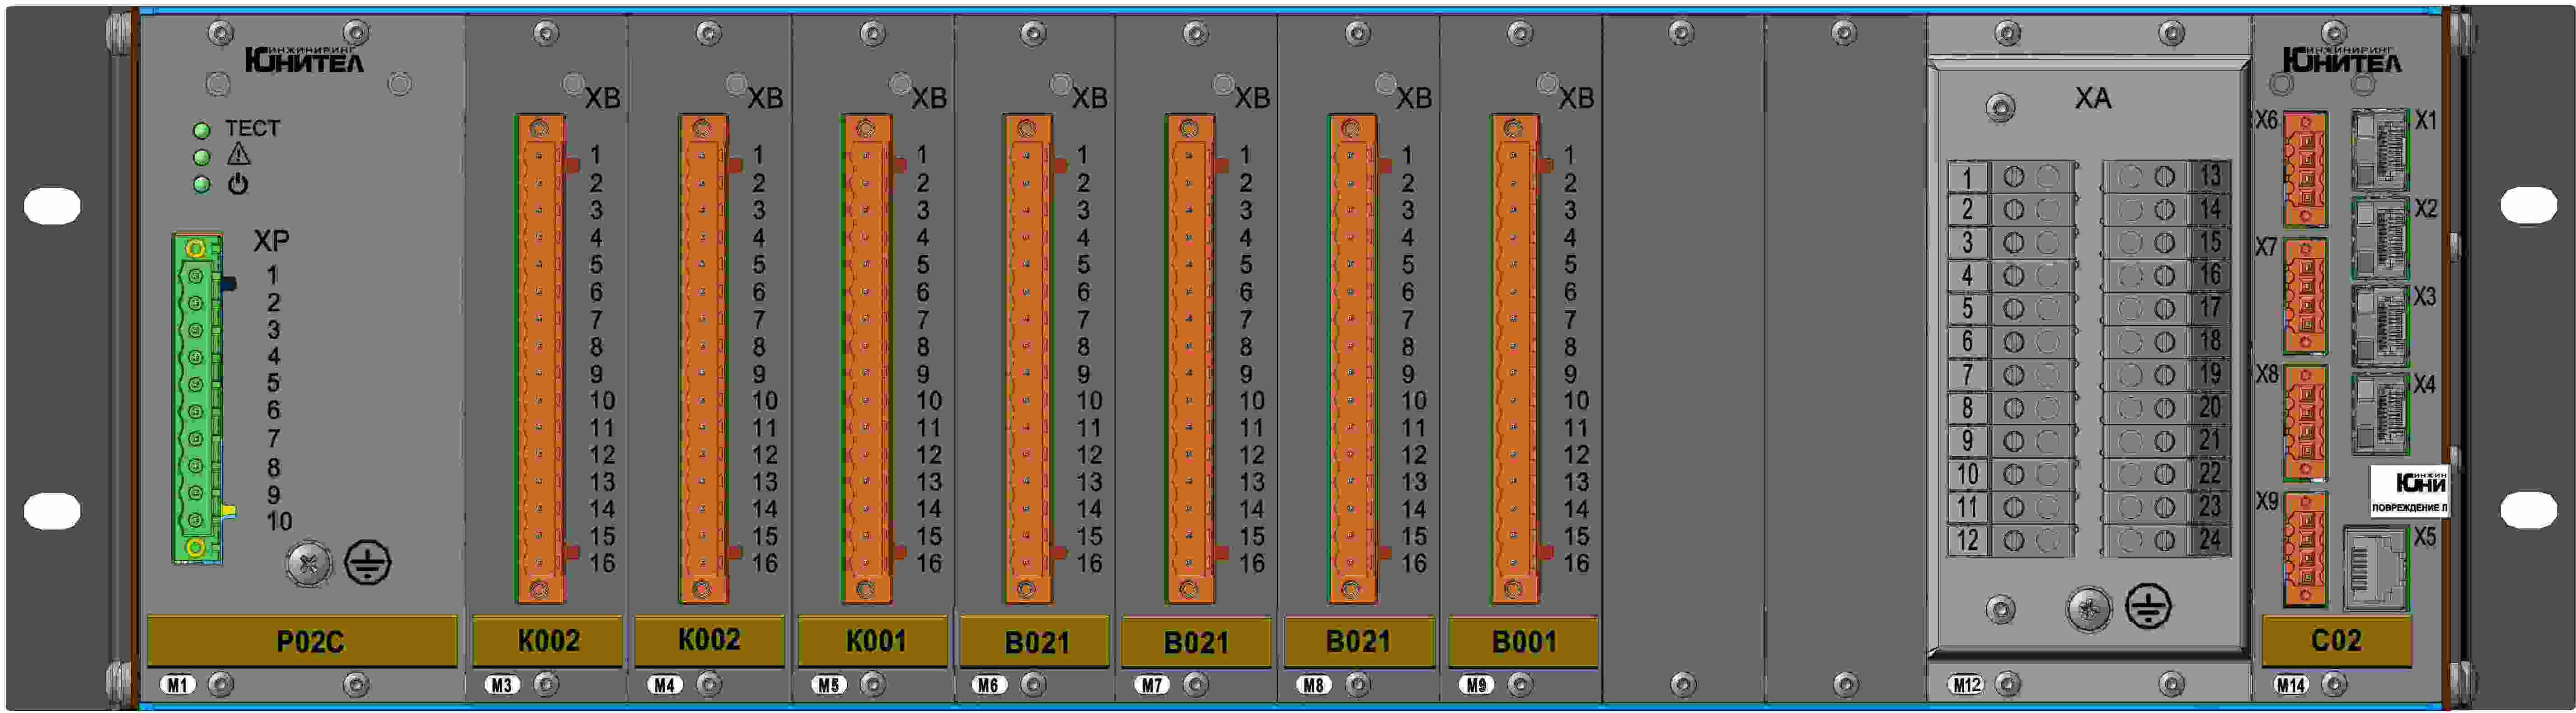
\includegraphics[width=1\textwidth,height=1\textheight,keepaspectratio]{img2.jpg}
\captionof{figure}{Вид устройства <<ЮНИТ-М319-ДЗТ2>> с размещением модулей по слотам (исполнение для I архитектуры)}\label{device:img1}
\end{figure}

\vspace{3mm}
\begin{figure}[H]
\centering
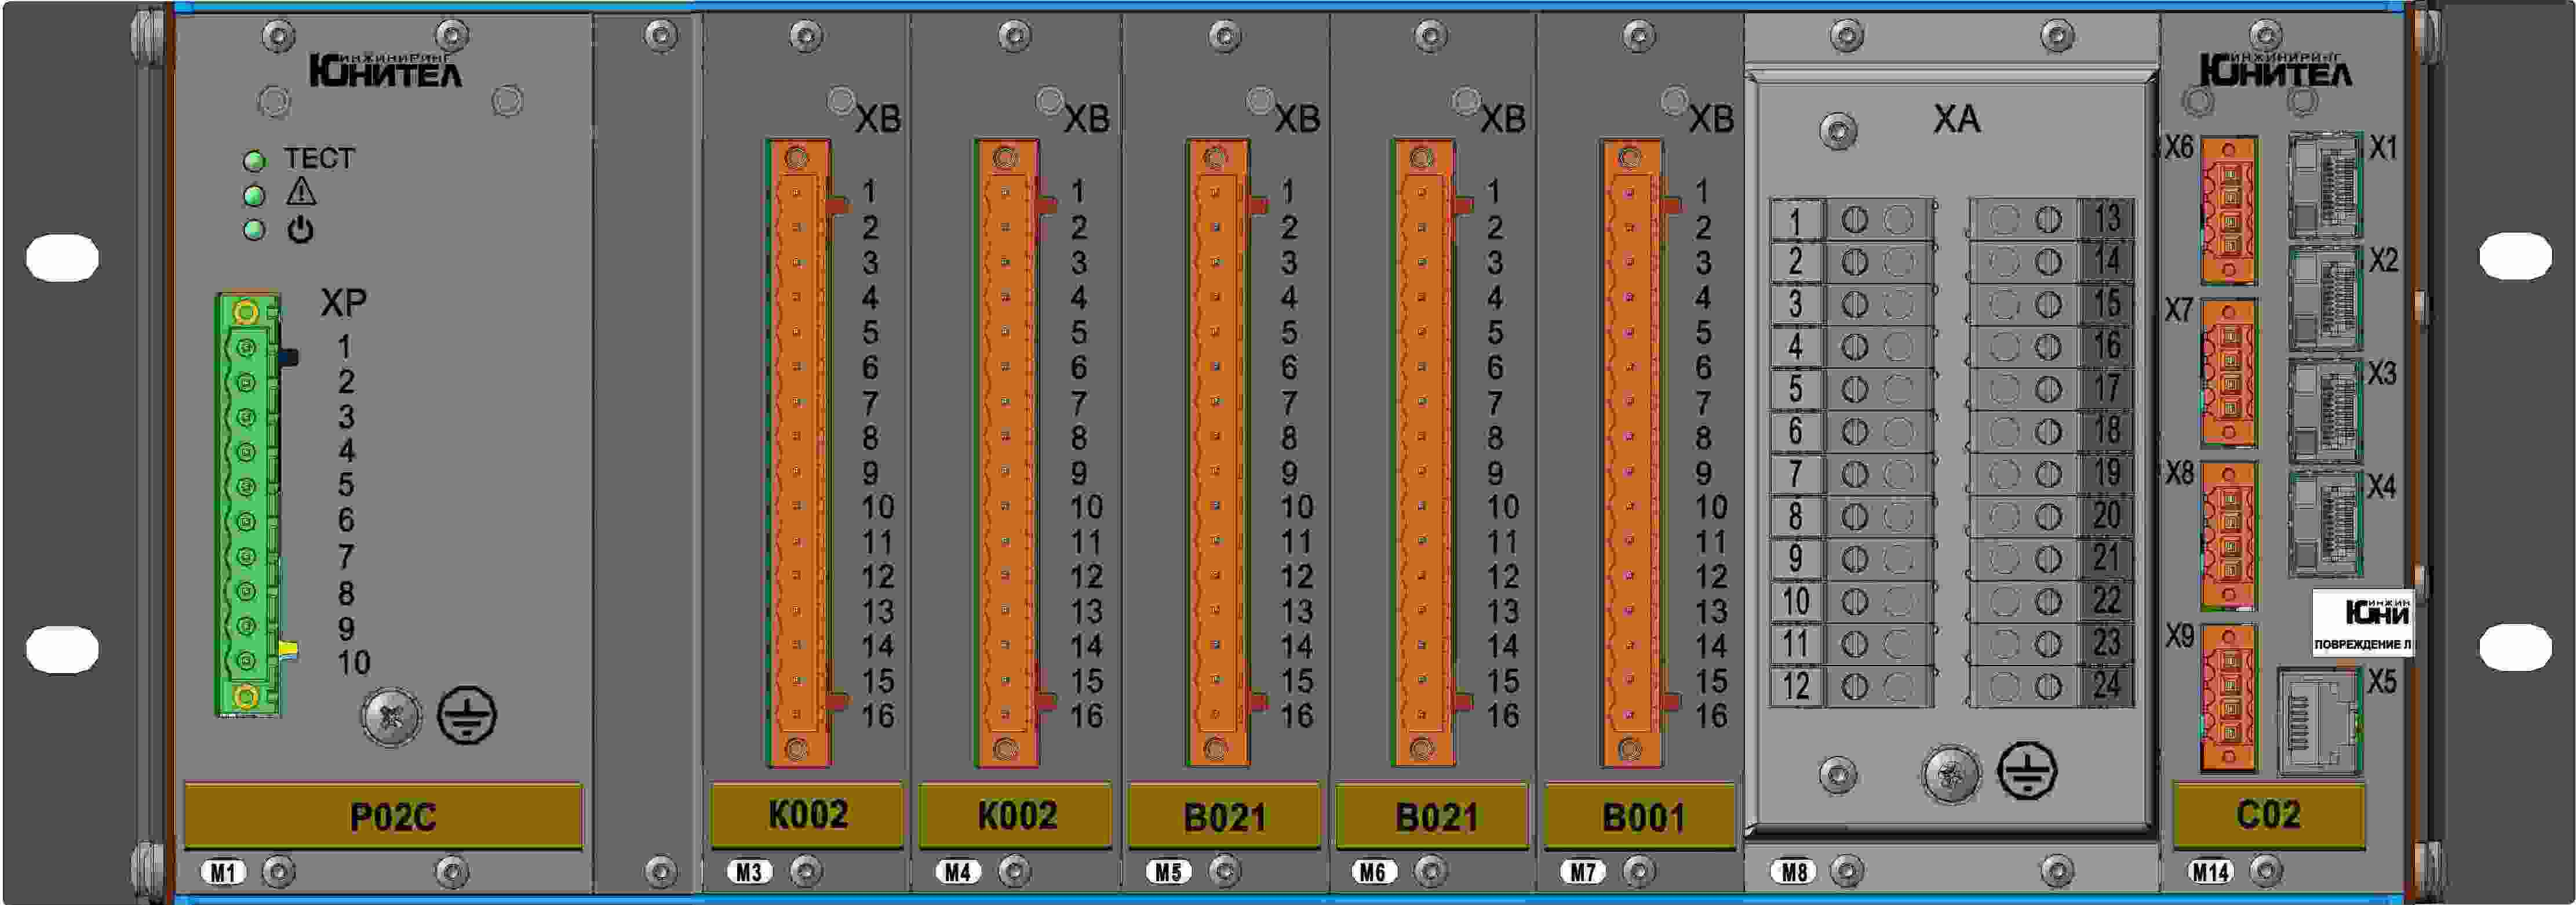
\includegraphics[width=0.8\textwidth,height=0.8\textheight,keepaspectratio]{img3.jpg}
\captionof{figure}{Вид устройства <<ЮНИТ-М314-ДЗТ2>> с размещением модулей по слотам (исполнение для II архитектуры)}\label{device:img2}
\end{figure}

\item
Перечень функций, реализованных в составе устройства приведен в таблице \ref{desc:tbl1}. Описание основных функций устройства приводится в разделе \ref{sec:funcs} данной документации. Подробное описание вспомогательных (сервисных) функций приведено в документации ЮТКБ.656122.609 РЭ <<Устройство защиты и автоматики серии <<ЮНИТ-М300>>. Руководство по эксплуатации общее>>.

\setlength{\extrarowheight}{0.05cm} % высота ячеек в таблице
\small
\begin{longtable}
    {|>{\centering\arraybackslash}m{3.2cm}|>{\centering\arraybackslash}m{13.7cm}|}
    \caption{Функции в составе устройства <<ЮНИТ-М319-ДЗТ2>>\hfill\vspace{-0.5\baselineskip}}\label{desc:tbl1}\\ 
    \hhline{|-|-|}
    \rowcolor{gray!30}
    Группа функций & Примечание \\ 
    \hhline{|-|-|}
    \endfirsthead

    \caption*{\hspace{3pt}\emph{Продолжение таблицы \ref{desc:tbl1}\hfill\vspace{-0.5\baselineskip}}} \\ % сделано по ГОСТ 2.105 п.6.8.7
    \hhline{|-|-|}
    \rowcolor{gray!30}
    Группа функций & Примечание \\ 
    \hhline{|-|-|}
    \endhead
    \hhline{|-|-|}

    \endfoot
    \endlastfoot

    \centering Основные функции & \flushleft\arraybackslash Основные защиты трансформатора (дифференциальная, газовая),
    технологические защиты трансформатора, УРОВ ВН трансформатора  \\  \hline

    \multirow{7}{*}{\centering Сервисные функции} & \flushleft\arraybackslash Сигнализация (обеспечение ввода служебных дискретных сигналов о состоянии оборудования шкафа РЗА, формирование отчетов по изменению состояния дискретных внешних и внутренних сигналов и выдачу отчетов в АСУ~ТП, формирование и выдачу сигналов аварийной и предупредительной сигнализации в схему резервной сигнализации) \\ \cline{2-2}
    & \flushleft\arraybackslash  Осциллографирование и журналирование (запись доаварийных, аварийных и послеаварийных режимов с сохранением осциллограмм в энергонезависимой памяти устройства, запись о событиях по изменению конфигурации устройства, изменения состояния внутренних сигналов алгоритмов, обновление встраиваемого программного обеспечения и пр. с метками времени и описанием события в энергонезависимой памяти устройства) \\ \cline{2-2}
    & \flushleft\arraybackslash Самодиагностика (непрерывный оперативный контроль работоспособности в течение всего времени работ) \\ \cline{2-2}
    & \flushleft\arraybackslash Конфигурирование (задание/переключение уставок, ввод в работу / вывод из работы, изменение параметров самоописания устройства, перезагрузка устройства, ввод/вывод тестового режима, изменение режима работы информационных сервисов, возможность переопределения связей входных и выходных логических сигналов алгоритмов устройства с дискретными входами, выходными реле, светодиодными индикаторами и функциональными клавишами управления) \\ \cline{2-2}
    & \flushleft\arraybackslash Тестовый режим (обработка принятых сигналов и отправка отчетов с установленным флагом <<Тест>>) \\ \cline{2-2}
    & \flushleft\arraybackslash Самоописание (предоставление данных об устройстве посредством устройства <<ЮНИТ-ИЧМ>> и сервисную программное обеспечение <<ЮНИТ-СЕРВИС>>) \\ \cline{2-2}
    & \flushleft\arraybackslash Синхронизация времени (календарь и часы реального времени, синхронизируемые от персонального компьютера или от АСУ~ТП) \\ \hhline{|-|-|}

\end{longtable}
\setlength{\extrarowheight}{0.0cm} % возврат параметра высота ячеек в таблице
\normalsize

\end{enumerate}

\color{uniblue}\subsection{Устройство и работа}\color{black}

\begin{enumerate}[label=\arabic{section}.\arabic{subsection}.\arabic*, labelsep=4pt, leftmargin=0pt, itemindent=57pt]
\item
Описание функций релейной защиты и автоматики в составе устройства, а также их функциональные схемы и уставки приводятся в разделе \ref{sec:funcs}. Общая функционально-структурная схема взаимосвязей функций, дискретных входов и выходов устройства приведена в приложении \ref{app:fsu}. Принятые обозначения элементов схем приведены в приложении \ref{app:func_desc}.
\item
Система самодиагностики устройства выполняет тесты в полном объеме при включении устройства, а также непрерывно в фоновом режиме.
Системой самодиагностики устройства в автоматическом режиме контролируются следующие параметры:
\begin{itemize}
\item состояние аппаратной части устройства, в том числе: АЦП модулей ввода аналоговых сигналов, блока питания, ОЗУ, ПЗУ, процессора, модулей дискретных входов, модулей дискретного управления, вспомогательных модулей;
\item температурный режим устройства;
\item состояние синхронизации времени;
\item сохранность исполняемого программного кода (целостность ПО);
\item состояние измерительных цепей;
\item исправность используемых каналов связи.
\end{itemize}
\item
Система самодиагностики фиксирует критические неисправности (<<Неисправность>>) и некритические ошибки (<<Ошибка>>). В случае появления критической неисправности активируется внутренний сигнал <<Критическая неисправность>>, замыкаются контакты реле IRF, прекращается работа алгоритмов основных функций в составе устройства, это состояние устройства сигнализируется свечением светодиода <<Неисправность>> и отсутствием свечения светодиода <<Готовность>>. В случае появления некритической ошибки активируется внутренний сигнал <<Некритическая ошибка>>, алгоритмы основных функций в составе устройства продолжают работать, это состояние устройства сигнализируется свечением светодиода <<Неисправность>> и отсутствием свечения светодиода <<Готовность>>. Подробное описание системы самодиагностики приводится в документации ЮТКБ.656122.609 РЭ <<Устройство защиты и автоматики серии <<ЮНИТ-М300>>. Руководство по эксплуатации общее>>.

\item
Для типоисполнения <<ЮНИТ-М314>> предусматривается установка модулей в любой из слотов с <<М3>> по <<М7>>:
\begin{itemize}
    \item выходных реле типа <<К001>> или <<К002>>;
    \item дискретных входов типа <<В001>> или <<В021>>.
\end{itemize}
\item
Для типоисполнения «ЮНИТ-М319» предусматривается установка модулей в любой из слотов с <<М3>> по <<М11>>:
\begin{itemize}
    \item выходных реле типа <<К001>>, <<К002>>;
    \item дискретных входов типа <<В001>> или <<В021>>.
\end{itemize}
\item
Типовое подключение входных сигналов функций к дискретным входам и выходным реле в составе устройства показано на рисунках приложения \ref{app:inouts} и \ref{app:inouts2}. 

\item
В устройстве установливается измерительный модуль в зависимости от карты заказа, например модуль <<М090>> (в котором предусмотрено девять каналов для измерения переменного тока), в устройстве <<ЮНИТ-М314>> занимает место в слотах <<М08>>, <<М09>>, а в устройстве <<ЮНИТ-М319>> занимает место в слотах <<М12>>, <<М13>>. Типовое подключение входных аналоговых сигналов к модулю аналоговых входов в составе устройства показано на рисунках приложения \ref{app:analogs}.

\item
Подробное описание параметров настроек и технических характеристик модулей дискретных входов, модулей дискретного управления и измерительных модулей приводится в документации ЮТКБ.656122.609 РЭ <<Устройство защиты и автоматики серии <<ЮНИТ-М300>>. Руководство по эксплуатации общее>>.

\item
В устройствах с поддержкой протокола передачи данных МЭК 61850 в качестве входных сигналов ФСУ могут быть использованы данные из GOOSE-сообщений, на которые оформлена подписка. Количество сигналов GOOSE, получаемых от интеллектуальных устройств, в данном типоисполнении устройства равно 12 шт.
\item
Сигналы из GOOSE-сообщений проходят предварительную обработку перед тем как попасть в <<Блок объединительный>> и далее в ФСУ (см. приложение \ref{app:fsu}).
В предварительную обработку входят следующие операции:
\begin{itemize}
\item проверка качества принимаемого сигнала;
\item алгоритм обработки резервирования GOOSE-сообщений;
\item алгоритм обработки симуляции GOOSE-сообщений;
\item алгоритм обработки метки <<Test>> GOOSE-сообщений;
\item подстановка значения по умолчанию при <<плохом>> качестве данных, принимаемых из GOOSE-сообщений.
\end{itemize}
Подробнее о подписке на GOOSE-сообщения указано в RU.37182817.00001.02.34.01 – <<Программное обеспечение мониторинга и параметрирования <<ЮНИТ-СЕРВИС>>. Руководство пользователя>>.

\item 
В устройствах с поддержкой протокола передачи данных МЭК 61850 для связи со смежными устройствами может быть использован протокол GOOSE по МЭК 61850-8.1. Количество сигналов GOOSE-сообщений, передаваемых в смежные интеллектуальные устройства, зависит от типоисполнения ЮНИТ-М300, первичного оборудования и в общем случае составляет не менее 100 шт. Подробнее о публикации GOOSE-сообщений указано в RU.37182817.00001.02.34.01 – <<Программное обеспечение мониторинга и параметрирования <<ЮНИТ-СЕРВИС>>. Руководство пользователя>>.
\item
Устройство поддерживает два режима оперативного управления: местный и дистанционный. Выбор режима управления устройством производится посредством функциональной клавиши <<М/Д>> или по состоянию выбранного дискретного входа. В местном режиме игнорируются все команды управления с верхнего уровня АСУ ТП. Более подробно режимы устройства описаны в документации ЮТКБ.656122.609 РЭ <<Устройство защиты и автоматики серии <<ЮНИТ-М300>>. Руководство по эксплуатации общее>>.
\item
Для управления режимами работы основных функций (оперативный ввод/вывод, перевод на сигнал и пр.), а также для генерации различных сигналов сброса функций (сброс триггеров фиксации неисправности цепей газовых и технологических защит, сброс счетчиков и пр.), применяются виртуальные ключи и кнопки. Подробное описание и сценарии работы виртуальных ключей и кнопок приведено в документации ЮТКБ.656122.609 РЭ <<Устройство защиты и автоматики серии <<ЮНИТ-М300>>. Руководство по эксплуатации общее>>. 
\item
В данном типоисполнении устройства реализовано четыре группы уставок. Подробное описание работы с группами уставок приведено в документации ЮТКБ.656122.609 РЭ <<Устройство защиты и автоматики серии <<ЮНИТ-М300>>. Руководство по эксплуатации общее>>.
\item
Устройство предусматривает возможность синхронизации внутренних часов реального времени несколькими способами:
\begin{itemize}
    \item по протоколу SNTP;
    \item по протоколу PTP;
    \item через дискретный вход устройства с использованием сигнала синхронизации 1PPS;
    \item {средствами стандартизованного протокола передачи данных.}
\end{itemize}
Подробное описание способов синхронизации времени устройства приведено в документации ЮТКБ.656122.609 РЭ <<Устройство защиты и автоматики серии <<ЮНИТ-М300>>. Руководство по эксплуатации общее>>.
\item
Устройство предусматривает возможность ведения журнала событий. Перечень сигналов, доступных для регистрации в журнале событий приведен, в приложении \ref{app:signals}. События безопасности записываются в отдельный журнал безопасности. Подробное описание параметров журналов событий приведено в документации ЮТКБ.656122.609 РЭ <<Устройство защиты и автоматики серии <<ЮНИТ-М300>>. Руководство по эксплуатации общее>>.
\item
Устройство предусматривает возможность осциллографирования событий. Перечень дискретных сигналов, доступных для регистрации аварийным осциллографом, приведен в приложении \ref{app:signals}. Подробное описание параметров встроенного регистратора аварийных событий приведено в документации ЮТКБ.656122.609 РЭ <<Устройство защиты и автоматики серии <<ЮНИТ-М300>>. Руководство по эксплуатации общее>>.
\item Перечень аналоговых сигналов, доступных для регистрации аварийным осциллографом, приведен в таблице \ref{osz:tbl1}.

\setlength{\extrarowheight}{0.05cm}
\small
\begin{longtable}{|>{\centering\arraybackslash}m{6.8cm}|>{\centering\arraybackslash}m{2cm}|>{\centering\arraybackslash}m{5.3cm}|>{\centering\arraybackslash}m{2cm}|}
\caption{Перечень аналоговых сигналов, доступных для регистрации аварийным осциллографом\hfill\vspace{-0.5\baselineskip}}\label{osz:tbl1}\\ 
\hline
\rowcolor{gray!30}
Описание аналогового сигнала & Канал & Наименование  & Пуск РАС \\ 
\hline
\endfirsthead
\caption*{\hspace{3pt}\emph{Продолжение таблицы \ref{osz:tbl1}\hfill\vspace{-0.5\baselineskip}}} \\ % сделано по ГОСТ 2.105 п.6.8.7
\hline
\rowcolor{gray!30}
Описание аналогового сигнала & Канал & Наименование  & Пуск РАС \\ 
\endhead
\endfoot
\endlastfoot

\raggedright Фазные токи ВН & \centering 1 & \centering Ia\_{\text{ВН}}  & \centering\arraybackslash + \\
\hline
\raggedright >>             & \centering 2 & \centering Ib\_{\text{ВН}}  & \centering\arraybackslash + \\
\hline
\raggedright >>             & \centering 3 & \centering Ic\_{\text{ВН}}  & \centering\arraybackslash + \\
\hline

\raggedright Фазные токи НН1 & \centering 4 & \centering Ia\_{\text{НН1}}  & \centering\arraybackslash + \\
\hline
\raggedright >>              & \centering 5 & \centering Ib\_{\text{НН1}}  & \centering\arraybackslash + \\
\hline
\raggedright >>              & \centering 6 & \centering Ic\_{\text{НН1}}  & \centering\arraybackslash + \\
\hline

\raggedright Фазные токи НН2 & \centering 7 & \centering Ia\_{\text{НН2}}  & \centering\arraybackslash + \\
\hline
\raggedright >>              & \centering 8 & \centering Ib\_{\text{НН2}}  & \centering\arraybackslash + \\
\hline
\raggedright >>              & \centering 9 & \centering Ic\_{\text{НН2}}  & \centering\arraybackslash + \\
\hline

\raggedright Вычисленный ток ОП ВН & \centering 10 & \centering I2\_{\text{ВН}}  & \centering\arraybackslash + \\
\hline
\raggedright Вычисленный ток НП ВН & \centering 11 & \centering 3I0\_{\text{ВН}}  & \centering\arraybackslash + \\
\hline

\raggedright Вычисленный ток ОП НН1 & \centering 12 & \centering I2\_{\text{НН1}}  & \centering\arraybackslash + \\
\hline
\raggedright Вычисленный ток НП НН1 & \centering 13 & \centering 3I0\_{\text{НН1}}  & \centering\arraybackslash + \\
\hline

\raggedright Вычисленный ток ОП НН2 & \centering 14 & \centering I2\_{\text{НН2}}  & \centering\arraybackslash + \\
\hline
\raggedright Вычисленный ток НП НН2 & \centering 15 & \centering 3I0\_{\text{НН2}}  & \centering\arraybackslash + \\
\hline

\raggedright Дифференциальные токи & \centering 16 & \centering Ia\_{\text{дифф}}  & \centering\arraybackslash + \\
\hline
\raggedright >>                    & \centering 17 & \centering Ib\_{\text{дифф}}  & \centering\arraybackslash + \\
\hline
\raggedright >>                    & \centering 18 & \centering Ic\_{\text{дифф}}  & \centering\arraybackslash + \\
\hline

\raggedright Тормозные токи & \centering 19 & \centering Ia\_{\text{торм}}  & \centering\arraybackslash - \\
\hline
\raggedright >>             & \centering 20 & \centering Ib\_{\text{торм}}  & \centering\arraybackslash - \\
\hline
\raggedright >>              & \centering 21 & \centering Ic\_{\text{торм}}  & \centering\arraybackslash - \\
\hline

\end{longtable}
\normalsize
\setlength{\extrarowheight}{0.0cm}

\item В устройстве реализована поддержка режима тестирования <<Тест>> в объеме требований стандартов МЭК 61850. Особенности перевода устройства в режим тестирования и функциональности устройства в этом режиме описаны в документации ЮТКБ.656122.609 РЭ <<Устройство защиты и автоматики серии <<ЮНИТ-М300>>. Руководство по эксплуатации общее>>.

\item\sloppy Описание и настройки доступных портов и интерфейсов связи приводится в документации ЮТКБ.656122.609 РЭ <<Устройство защиты и автоматики серии <<ЮНИТ-М300>>. Руководство по эксплуатации общее>>.

\item Устройство имеет встроенную реализацию правил разграничения прав доступа, для этого в устройстве существует ролевая модель разграничения прав доступа.
В устройстве предусмотрены следующие роли:
\begin{itemize}
    \item Гость (пароль не требуется, доступен просмотр данных устройства);
    \item Дежурный;
    \item Инженер;
    \item Офицер (сотрудник) безопасности;
    \item Администратор (пароль <<АААА>> (кириллица), учетная запись предназначена для первоначального конфигурирования штатного профиля пользователей).
\end{itemize}
Все пользователи делятся на непривилегированных (роль Гость) и привилегированных (все остальные роли).
\item
Предустановленные пользователи с именами Гость и Администратор не подлежат удалению и принудительной блокировке, их роли не подлежат изменению. Гость используется как роль по умолчанию для доступа к просмотру данных устройства в режиме чтение без запроса аутентификационных данных пользователя. Администратор необходим для добавления/удаления других пользователей, установки им соответствующих ролей и установке/изменении паролей пользователей.
\item
После перезагрузки устройства подключенная сессия привилегированного пользователя сбрасывается. Устройство запускается с сеансом непривилегированного пользователя (роль Гость).
Подробное описание ролей и доступных полномочий и ограничений для каждой из ролей приведено в документации ЮТКБ.656122.609 РЭ <<Устройство защиты и автоматики серии <<ЮНИТ-М300>>. Руководство по эксплуатации общее>>.

\end{enumerate}

\color{uniblue}\subsection{Средства измерения, инструмент и принадлежности}\color{black}
Перечень оборудования и средств измерения, рекомендуемый для проведения эксплуатационных проверок устройства, приведен в документации ЮТКБ.656122.609 РЭ <<Устройство защиты и автоматики серии <<ЮНИТ-М300>>. Руководство по эксплуатации общее>>.

\color{uniblue}\subsection{Маркировка и пломбирование}\color{black}
Сведения по маркировке и пломбировании устройства приведены в документации ЮТКБ.656122.609 РЭ <<Устройство защиты и автоматики серии <<ЮНИТ-М300>>. Руководство по эксплуатации общее>>.

\color{uniblue}\subsection{Упаковка}\color{black}
Сведения по упаковке устройства приведены в документации ЮТКБ.656122.609 РЭ <<Устройство защиты и автоматики серии <<ЮНИТ-М300>>. Руководство по эксплуатации общее>>.
\newpage
\color{uniblue}\section[Основные функции]{Основные функции}\label{sec:funcs}
\color{black}

\needspace{4\baselineskip}
\color{uniblue}{\subsection{Общие сведения}}
\color{black}

\begin{enumerate}[label=\arabic{section}.\arabic{subsection}.\arabic*, labelsep=4pt, leftmargin=0pt, itemindent=57pt]
    
\item
При вводе в работу устройство постоянно отслеживает состояние подключенных к нему аналоговых и дискретных сигналов. Из значений, полученных АЦП, при помощи расчетов и, при необходимости, цифровой фильтрации выделяются среднеквадратичные и/или мгновенные величины (фазных токов, дифференциальных и тормозных токов, гармонических составляющих токов), необходимые для работы функций в составе устройства.
\item
Оперативный вывод всех функций в составе устройства из работы происходит при появлении активного сигнала <<Вывод терминала>>.
\item
Значения задаваемых параметров для токов дифференциальных токовых функций в таблицах параметров настройки, приведены к базисному току трансформатора и указаны в относительных единицах, значения задаваемых параметров для токов остальных функций в таблицах параметров настройки приведены по отношению к номинальному значению тока аналогового входа и указываются в относительных единицах (о.е).  
\item
Коэффициенты возврата максимальных измерительных органов заданы равными 0,95, коэффициенты возврата минимальных измерительных органов заданы равными 1,05 (если в описании функции не указано другое значение).

\item
Основные характеристики функциональных блоков:
\begin{itemize}
    \item погрешность измерительных органов тока и напряжения (в том числе ИО по симметричным составляющим) не более 2,5\%, на границе частот 45 Гц и 55 Гц не более 5\%;
    \item время срабатывания ИО тока при повышении тока скачком от 0 до 2Iуст. не более 40 мс;
    \item время возврата реле ИО тока при снижении тока скачком от 2Iуст. до 0 не более 40 мс;
    \item время срабатывания ИО напряжения при повышении напряжения скачком от 0 до 2Uуст не более 40 мс;
    \item время возврата ИО напряжения при сбросе напряжения скачком от 2Uуст до 0 должно быть не более 40 мс; 
    \item погрешность выдержки времени -- не более 40 мс при выдержках менее 1,5 с и не более 2\% от уставки при выдержках времени выше 1,5 с.
\end{itemize}
Специфические требования к характеристикам функциональных блоков приведены в описаниях соответствующих функций в данном разделе.

\item
Общая схема взаимосвязей между описанными в данном разделе функциями, входными и выходными сигналами устройства приведена в приложении \ref{app:fsu}.
Сводный перечень сигналов, формируемых устройством в процессе работы, приведен в таблице \ref{appA:tbl1} приложения \ref{app:signals}.

\end{enumerate}
\color{uniblue}{\subsection{Дифференциальная токовая защита трансформатора (ДЗТ)}}
\color{black}

\begin{enumerate}[label=\arabic{section}.\arabic{subsection}.\arabic{enumi}, labelsep=4pt, leftmargin=0pt, itemindent=57pt, itemsep=0pt, parsep=5pt] % если что можно крутить itemsep
\item Общие сведения

\begin{enumerate}[label=\arabic{section}.\arabic{subsection}.\arabic{enumi}.\arabic*, labelsep=4pt, leftmargin=0em, itemindent=65pt, parsep=0pt]

\item
Дифференциальная токовая защита применяется в качестве основной защиты двухобмоточного или трехобмоточного силового трансформатора. ДЗТ обладает абсолютной селективностью и высоким быстродействием. Работа дифференциальных токовых функций не зависит от режима заземления нейтрали сети, и, следовательно, ДЗТ  может быть использована в качестве основной защиты от всех видов коротких замыканий. Функциональный блок содержит две независимые друг от друга защитные функции:
\begin{itemize}
\item дифференциальный токовый орган с торможением (ДТЗт);
\item дифференциальная токовая отсечка (ДТО).
\end{itemize}
\item
Функциональный блок <<ДЗТ>> также включает в себя вспомогательные функции, необходимые для правильной работы в различных режимах:
\begin{itemize}
    \item детектор второй гармоники (Д2Г);
    \item детектор пятой гармоники (Д5Г);
    \item функция блокировки при внешний коротких замыканиях (БВКЗ);
    \item функция контроля токовых цепей по величине небаланса (КЦТнеб).
\end{itemize}

\item
Основные характеристики функционального блока <<ДЗТ>>:
\begin{itemize}
    \item полное время срабатывания чувствительной ступени ДЗТ при дифференциальном токе более двухкратного тока уставки, в том числе с учетом наличия апериодической составляющей, с учетом времени срабатывания выходного реле - не более 50 мс.
\end{itemize}

\item
Оперативный вывод функционального блока <<ДЗТ>> из работы происходит при появлении активного сигнала на входе <<ОВ ДЗТ>>, при этом осуществляется вывод защитных функций <<ДТО>> и <<ДТЗт>>. 
\end{enumerate}
\item
Принцип работы дифференциальной защиты основан на первом правиле Кирхгофа. Защищаемый объект рассматривается как электрический узел, а его связи с электрической сетью как ветви узла.


\item  Цифровое выравнивание, исключение токов нулевой последовательности

\begin{enumerate}[label=\arabic{section}.\arabic{subsection}.\arabic{enumi}.\arabic*, labelsep=4pt, leftmargin=0em, itemindent=65pt, parsep=0pt]

\item
Силовые трансформаторы имеют различные группы соединений обмоток, при этом у измерительных ТТ, установленных по сторонам защищаемого трансформатора различные номинальные значения первичных и вторичных токов, поэтому, прежде чем выполнить сравнение фазных токов каждой из сторон трансформатора, необходимо выполнить выравнивание измеряемых токов по модулю (амплитуде), по фазе и, при необходимости, выполнить фильтрацию токов нулевой последовательности.
Устройство по заданным параметрам осуществляет выравнивание измеренных токов сторон в соответствии с формулой:

\begin{equation*}
\begin{bmatrix}
I_{A,n*}\\ 
I_{B,n*}\\ 
I_{C,n*}
\end{bmatrix}= k_{AM,n}\times \begin{bmatrix}
M_{11,n} & M_{12,n} & M_{13,n}\\ 
M_{21,n} & M_{22,n} & M_{23,n}\\ 
M_{31,n} & M_{32,n} & M_{33,n}
\end{bmatrix}\times \begin{bmatrix}
I_{A,n}\\ 
I_{B,n}\\ 
I_{C,n}
\end{bmatrix},
\end{equation*}
\begin{eqexpl}[25mm]
\item{$n$}индекс, обозначающий сторону (плечо) ДЗТ;
\item{$k_{AM,n}$}коэффициент амплитудного выравнивания;
\item{$I_{A,n},I_{B,n},I_{C,n}$}измеренные фазные токи стороны $n$;
\item{$M_{11,n}\dots M_{33,n} $}коэффициенты матрицы компенсации фазового сдвига в соответствие  с группой соединения обмоток трансформатора.
\end{eqexpl}

\item

Расчет коэффициента амплитудного выравнивания ($k_{AM,n}$) производится по задаваемым параметрам величин номинальных значений силового трансформатора и измерительных трансформаторов тока в соответствии с выражениями:


\begin{equation*}
k_{AM,n}= \frac{I_{\textsl{перв,n}}\cdot  I_{\textsl{ном.терм,n}} }{I_{\textsl{баз,n}}\cdot I_{\textsl{втор,n}}\cdot k_{\textsl{сх,n}}},
\end{equation*}
\begin{equation*}
I_{\textsl{баз,n}}=\frac{S_{\textsl{баз}}}{\sqrt{3} \cdot U_{\textsl{баз,n}} },
\end{equation*}
\begin{eqexpl}[25mm]
\item{$n$} индекс, обозначающий сторону (плечо) ДЗТ;
\item{$I_{\textsl{перв,n}}$}номинальный первичный ток ТТ стороны $n$;
\item{$I_{\textsl{втор,n}}$}номинальный вторичный ток ТТ стороны $n$;
\item{$I_{\textsl{ном.терм,n}}$}номинальное значение тока аналоговых входов устройства, подключенных к ТТ стороны $n$;
\item{$k_{\textsl{сх,n}}$}коэффициент, учитывающий схему соединения обмоток ТТ стороны~$n$. Данный параметр принимается равным 1, когда ТТ стороны $n$ собраны в звезду, или равным $\sqrt{3}$, когда ТТ стороны $n$ собраны в треугольник. Коэффициенты схемы соединения ТТ для каждой из сторон задается уставками <<KсхемСт1>>, <<KсхемСт2>>, <<KсхемСт3>>;
\item{$S_{\textsl{баз}}$}базисная мощность, равная номинальной мощности силового трансформатора;
\item{$U_{\textsl{баз,n}}$}базисное напряжение, равное номинальному напряжению обмотки трансформатора соответствующей стороне $n$.
\end{eqexpl}

\item 
Для компенсации фазового сдвига, обусловленного различными группами соединения обмоток трансформатора для каждой из сторон предусмотрены задаваемые параметры (<<Nсх1>>, <<Nсх2>>, <<Nсх3>>). Значения данных параметров (от 0 до 11) определяют коэффициенты матрицы $M_{11,n}\dots M_{33,n}$ в соответствие с таблицей \ref{dzt:tbl0}.


\item 
Для обмоток силового трансформатора, соединенных в звезду с заземленной нейтралью, и, если не используется других мер исключения токов нулевой последовательности (соединение вторичных обмоток ТТ в треугольник) всегда рекомендуется предусматривать исключение составляющих нулевой последовательности из фазных токов. Компенсация токов нулевой последовательности сторон задается параметрами <<Компенс3I0ст1>>, <<Компенс3I0ст2>>, <<Компенс3I0ст3>>. В случае, когда параметр компенсации токов нулевой последовательности для стороны равен <<0>> (без компенсации тока $3I0$), то в формуле для выравнивания измеряемых токов сторон применяются коэффициенты матрицы M (см. таблицу \ref{dzt:tbl0}). В случае, когда параметр компенсации токов нулевой последовательности для стороны равен <<1>> (с компенсацией токов $3I0$), то в формуле для выравнивания измеряемых токов сторон применяются коэффициенты матрицы M0 (см. таблицу \ref{dzt:tbl0}).

\small
\begin{longtable}{|>{\centering\arraybackslash}m{1.7cm}|>{\centering\arraybackslash}m{4cm}|>{\centering\arraybackslash}m{3cm}|>{\centering\arraybackslash}m{4cm}|>{\centering\arraybackslash}m{3cm}|}
\caption{Компенсация группы соединения \hfill\vspace{-0.5\baselineskip}}\label{dzt:tbl0}\\
\hhline{|-|-|-|-|-|}
\rowcolor{gray!30}
\multicolumn{1}{|c|}{} & \multicolumn{2}{c|}{Без компенсации токов 3I0} & \multicolumn{2}{c|}{С компенсацией токов 3I0} \\
\hhline{|-|-|-|-|-|}
\rowcolor{gray!30}
Векторная группа & Матрица М & Группы соединений обмоток & Матрица М0 & Группы соединений обмоток \\ 
\hhline{|-|-|-|-|-|}
\endfirsthead

\caption*{\hspace{3pt}\emph{Продолжение таблицы \ref{dzt:tbl0}\hfill\vspace{-0.5\baselineskip}}} \\ % сделано по ГОСТ 2.105 п.6.8.7
\hhline{|-|-|-|-|-|}
\rowcolor{gray!30}
\multicolumn{1}{|c|}{} & \multicolumn{2}{c|}{Без компенсации токов 3I0} & \multicolumn{2}{c|}{С компенсацией токов 3I0} \\
\hhline{|-|-|-|-|-|}
\rowcolor{gray!30}
Векторная группа & Матрица М & Группы соединений обмоток & Матрица М0 & Группы соединений обмоток \\ 
\hhline{|-|-|-|-|-|}
\endhead
\hhline{|-|-|-|-|-|}
\endfoot
\endlastfoot

\centering 0 & \centering $$\begin{vmatrix}1&0&0\\0&1&0\\0&0&1\end{vmatrix}$$ & \centering \parbox{1cm}{Yy0 Dd0} & \centering $$\displaystyle\frac{1}{3}\times \begin{vmatrix}2&-1&-1\\-1&2&-1\\-1&-1&2\end{vmatrix}$$ & \centering\arraybackslash \parbox{1cm}{Yyn0 YNy0} \\
\hline

\centering 1 & \centering $$\displaystyle\frac{1}{\sqrt{3}}\times\begin{vmatrix}2&-1&-1\\-1&2&-1\\-1&-1&2\end{vmatrix}$$ & \centering \parbox{1cm}{Yd1 Dy1} & \centering Равна матрице №1 & \centering\arraybackslash \parbox{1cm}{YNd1 Dyn1} \\
\hline

\centering 2 & \centering $$\begin{vmatrix}0&-1&0\\0&0&-1\\-1&0&0\end{vmatrix}$$ & \centering \parbox{1cm}{Yy2 Dd2} & \centering $$\displaystyle\frac{1}{3}\times \begin{vmatrix}1&-2&1\\1&1&-2\\-2&1&1\end{vmatrix}$$ & \centering\arraybackslash \parbox{1cm}{YNy2 Yyn2} \\
\hline

\centering 3 & \centering $$\displaystyle\frac{1}{\sqrt{3}}\times\begin{vmatrix}0&-1&1\\1&0&-1\\-1&1&0\end{vmatrix}$$ & \centering \parbox{1cm}{Yd3 Dy3} & \centering Равна матрице №3 & \centering\arraybackslash \parbox{1cm}{YNd3 Dyn3} \\
\hline

\centering 4 & \centering $$\begin{vmatrix}0&0&1\\1&0&0\\0&1&0\end{vmatrix}$$ & \centering \parbox{1cm}{Yy4 Dd4} & \centering $$\displaystyle\frac{1}{3}\times \begin{vmatrix}-1&-1&2\\2&-1&-1\\-1&2&-1\end{vmatrix}$$ & \centering\arraybackslash \parbox{1cm}{YNy4 Yyn4} \\
\hline

\centering 5 & \centering $$\displaystyle\frac{1}{\sqrt{3}}\times\begin{vmatrix}-1&0&1\\1&-1&0\\0&1&-1\end{vmatrix}$$ & \centering \parbox{1cm}{Yd5 Dy5} & \centering Равна матрице №5 & \centering\arraybackslash \parbox{1cm}{YNd5 Dyn5} \\
\hline

\centering 6 & \centering $$\begin{vmatrix}-1&0&0\\0&-1&0\\0&0&-1\end{vmatrix}$$ & \centering \parbox{1cm}{Yy6 Dd6} & \centering $$\displaystyle\frac{1}{3}\times \begin{vmatrix}-2&1&1\\1&-2&1\\1&1&-2\end{vmatrix}$$ & \centering\arraybackslash \parbox{1cm}{YNy6 Yyn6} \\
\hline

\centering 7 & \centering $$\displaystyle\frac{1}{\sqrt{3}}\times\begin{vmatrix}-1&1&0\\0&-1&1\\1&0&-1\end{vmatrix}$$ & \centering \parbox{1cm}{Yd7 Dy7} & \centering Равна матрице №7 & \centering\arraybackslash \parbox{1cm}{YNd7 Dyn7} \\
\hline

\centering 8 & \centering $$\begin{vmatrix}0&1&0\\0&0&1\\1&0&0\end{vmatrix}$$ & \centering \parbox{1cm}{Yy8 Dd8} & \centering $$\displaystyle\frac{1}{3}\times \begin{vmatrix}-1&2&-1\\-1&-1&2\\2&-1&-1\end{vmatrix}$$ & \centering\arraybackslash \parbox{1cm}{YNy8 Yyn8} \\
\hline

\centering 9 & \centering $$\displaystyle\frac{1}{\sqrt{3}}\times\begin{vmatrix}0&1&-1\\-1&0&1\\1&-1&0\end{vmatrix}$$ & \centering \parbox{1cm}{Yd9 Dy9} & \centering Равна матрице №9 & \centering\arraybackslash \parbox{1cm}{YNd9 Dyn9} \\
\hline

\centering 10 & \centering $$\begin{vmatrix}0&0&-1\\-1&0&0\\0&-1&0\end{vmatrix}$$ & \centering \parbox{1cm}{Yy10 Dd10} & \centering $$\displaystyle\frac{1}{3}\times \begin{vmatrix}1&1&-2\\-2&1&1\\1&-2&1\end{vmatrix}$$ & \centering\arraybackslash \parbox{1cm}{YNy10 Yyn10} \\
\hline

\centering 11 & \centering $$\displaystyle\frac{1}{\sqrt{3}}\times\begin{vmatrix}1&0&-1\\-1&1&0\\0&-1&1\end{vmatrix}$$ & \centering \parbox{1cm}{Yd11 Dy11} & \centering Равна матрице №11 & \centering\arraybackslash \parbox{1cm}{YNd11 Dyn11} \\
\hline

\end{longtable}
\normalsize

\end{enumerate}


\item\label{sec:dtzt} Дифференциальный токовый орган с торможением (ДТЗт)

\begin{enumerate}[label=\arabic{section}.\arabic{subsection}.\arabic{enumi}.\arabic*, labelsep=4pt, leftmargin=0em, itemindent=65pt, parsep=0pt]

\item
Характеристика срабатывания <<ДТЗт>> в координатах $I_{\textsl{диф}}$ и $I_{\textsl{торм}}$ представляет собой ломаную линию (см. рисунок \ref{dzt:char}), состоящую из трех участков. Данная характеристика срабатывания обеспечивает чувствительность <<ДТЗт>> при малых токах КЗ в зоне действия защиты.

\vspace{1mm}
\begin{figure}[H]
\centering
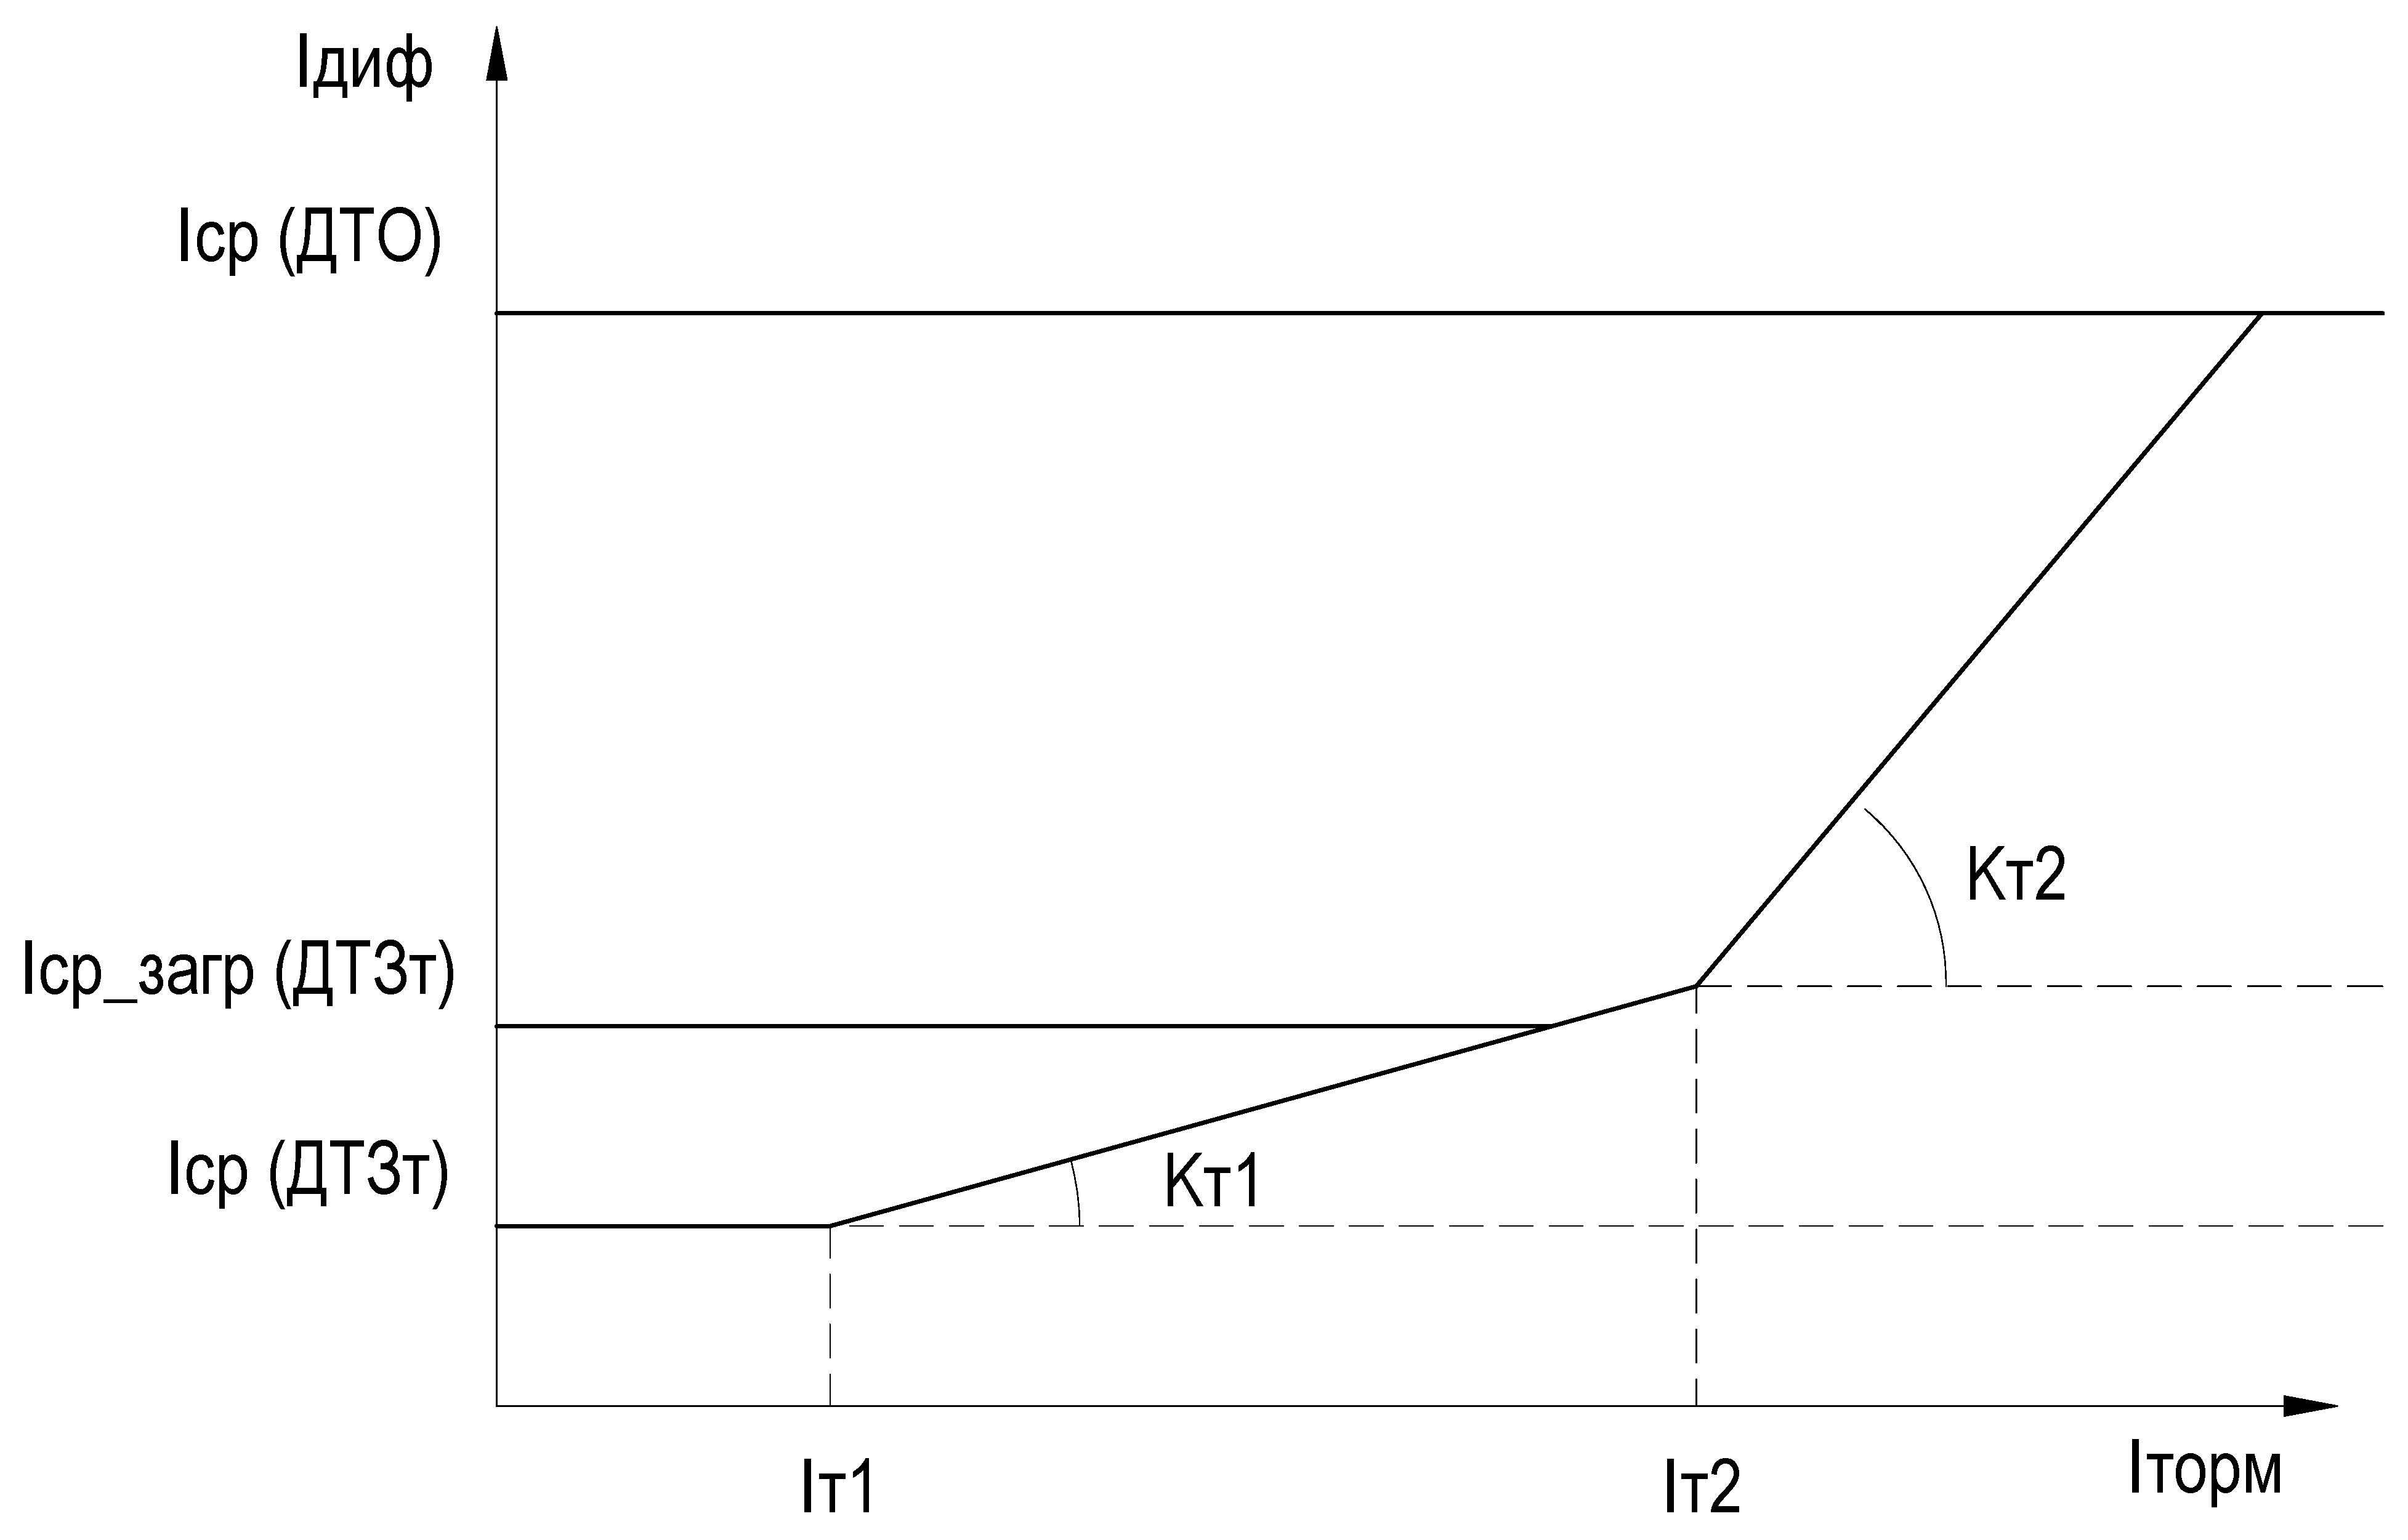
\includegraphics[width=0.6\textwidth,height=0.6\textheight,keepaspectratio]{img4.pdf}
\captionof{figure}{Характеристика срабатывания ДЗТ}\label{dzt:char}
\end{figure}

\item
Первый участок выполнен горизонтальным и определяется уставкой минимального дифференциального тока срабатывания <<Iср (ДТЗт)>>. Второй участок представлен в виде наклонной линии и определяется уставками начального тормозного тока <<Iт1>> и коэффициентом торможения\footnote{~Коэффициент торможения это отношение приращения дифференциального тока срабатывания к приращению тормозного тока.} <<Kт1>>. Третий участок представлен в виде наклонной линии и определяется уставками начального тормозного тока <<Iт2>> и коэффициентом торможения <<Kт2>>. Уставки для всех трех фаз задаются одинаковыми. Для исключения возможности излишнего срабатывания при насыщении измерительных ТТ на значениях тормозного тока выше <<Iт2>> в <<ДТЗт>> предусмотрена блокировка при внешних КЗ.
\item
Для каждой из фаз непрерывно выполняется расчет дифференциального и тормозного токов. Основной рабочей величиной ДЗТ является дифференциальный ток. В общем виде дифференциальный ток равен модулю геометрической суммы токов основных гармоник плеч, определенных с учетом коэффициентов выравниваний и компенсации токов нулевой последовательности (в случае необходимости) по формуле:

\begin{equation*}
I_{\textsl{диф.ph}} = \left | \sum_{n=1}^{m}I_{ph,n*} \right |,
\end{equation*}
\begin{eqexpl}[25mm]
\item{$ph$}контролируемая фаза (A,B,C);
\item{$I_{ph,n*}$}вектор тока основной гармоники $n$-го плеча, определенного с учетом коэффициентов выравниваний;
\item{$m$}число сторон (до трёх).
\end{eqexpl}

\item
Дифференциальные токи отдельных фаз определяются (в случае, если используется три стороны защищаемого объекта) по следующим формулам:  
\begin{equation*}
\begin{split}
I_{\textsl{диф.A}} = \left | I_{A,1*}+I_{A,2*}+I_{A,3*} \right |,\\
I_{\textsl{диф.B}} = \left | I_{B,1*}+I_{B,2*}+I_{B,3*} \right |,\\
I_{\textsl{диф.C}} = \left | I_{C,1*}+I_{C,2*}+I_{C,3*} \right |.
\end{split}
\end{equation*}

\item
В общем виде тормозной ток <<ДТЗт>> равен арифметической полусумме входных токов плеч, определенных с учетом коэффициентов выравниваний по формуле:
\begin{equation*}
I_{\textsl{торм.ph}} = \frac{1}{2} \sum_{n=1}^{m}\left |I_{ph,n*} \right |,
\end{equation*}
\begin{eqexpl}[25mm]
\item{$ph$}контролируемая фаза (A,B,C);
\item{$I_{ph,n*}$}вектор тока основной гармоники n-го плеча, определенного с учетом коэффициентов выравниваний;
\item{$m$}число сторон (до трёх).
\end{eqexpl}

\item
Тормозные токи отдельных фаз определяются (в случае, если используется три стороны защищаемого объекта) по следующим формулам:  
\begin{equation*}
\begin{split}
I_{\textsl{торм.A}} = \frac{1}{2}(\left | I_{A,1*}|+|I_{A,2*}|+|I_{A,3*} \right |),\\
I_{\textsl{торм.B}} = \frac{1}{2}(\left | I_{B,1*}|+|I_{B,2*}|+|I_{B,3*} \right |),\\
I_{\textsl{торм.C}} = \frac{1}{2}(\left | I_{C,1*}|+|I_{C,2*}|+|I_{C,3*} \right |).
\end{split}
\end{equation*}

\item
В случае попадания расчетных величин в зону срабатывания на время большее времени уставки <<Тср>> формируется сигнал срабатывания <<ДТЗт>>.

\item
Ввод <<ДТЗт>> в работу на этапе параметрирования устройства осуществляется программным переключателем SGF1 <<Ввод\_функции>>. Информация о введенной функции отображается выходным сигналом <<ДТЗт: Ввод>>.
\item
Функция <<ДТЗт>> может быть выведена из работы оперативно путем активации сигнала <<ОВ ДТЗт>>, что характеризуется активным состоянием сигнала <<ДТЗт: Оперативный вывод>> на выходе функции. 
\item
При активном состоянии входного сигнала <<ДТЗт~на~сигн>> действие отключающей логики переводится на сигнал.
\item
Программным переключателем SGF2 <<Реж\_блок>> возможен выбор режима блокировки <<ДТЗт>>: <<Без блокировки>>, <<Блокировка по второй гармонике>>, <<Блокировка по пятой гармонике>>, <<Блокировка по второй и пятой гармоникам>>.
\item
В алгоритме функции <<ДТЗт>> предусмотрена работа с дополнительным подтверждением от функции блокировки от внешних КЗ (<<БВКЗ>>) путем выбора состояния <<С контролем БВКЗ>> программного переключателя SGF3 <<Контр\_БВКЗ>>, описание работы функции <<БВКЗ>> приведено в подразделе \ref{sec:bvkz}.
\item
При выявлении неисправности в цепях ТТ, что определяется срабатыванием функции <<КЦТ>> по сторонам трансформатора (см. подраздел \ref{sec:kzt}) автоматически увеличивается уровень тока срабатывания горизонтального участка тормозной характеристики для снижения вероятности ложного срабатывания <<ДТЗт>> в режиме протекания токов нагрузки путем загрубления уставки <<ДТЗт>> до уровня <<Iср\_загр>> (см. рисунок \ref{dzt:char}).
\item
Алгоритм работы <<ДТЗт>> выполнен в соответствии с рисунком \ref{dzt:img1}. В таблице \ref{dzt:tbl1} приведены параметры, необходимые для настройки функции <<ДТЗт>>.

\vspace{1mm}
\begin{figure}[H]
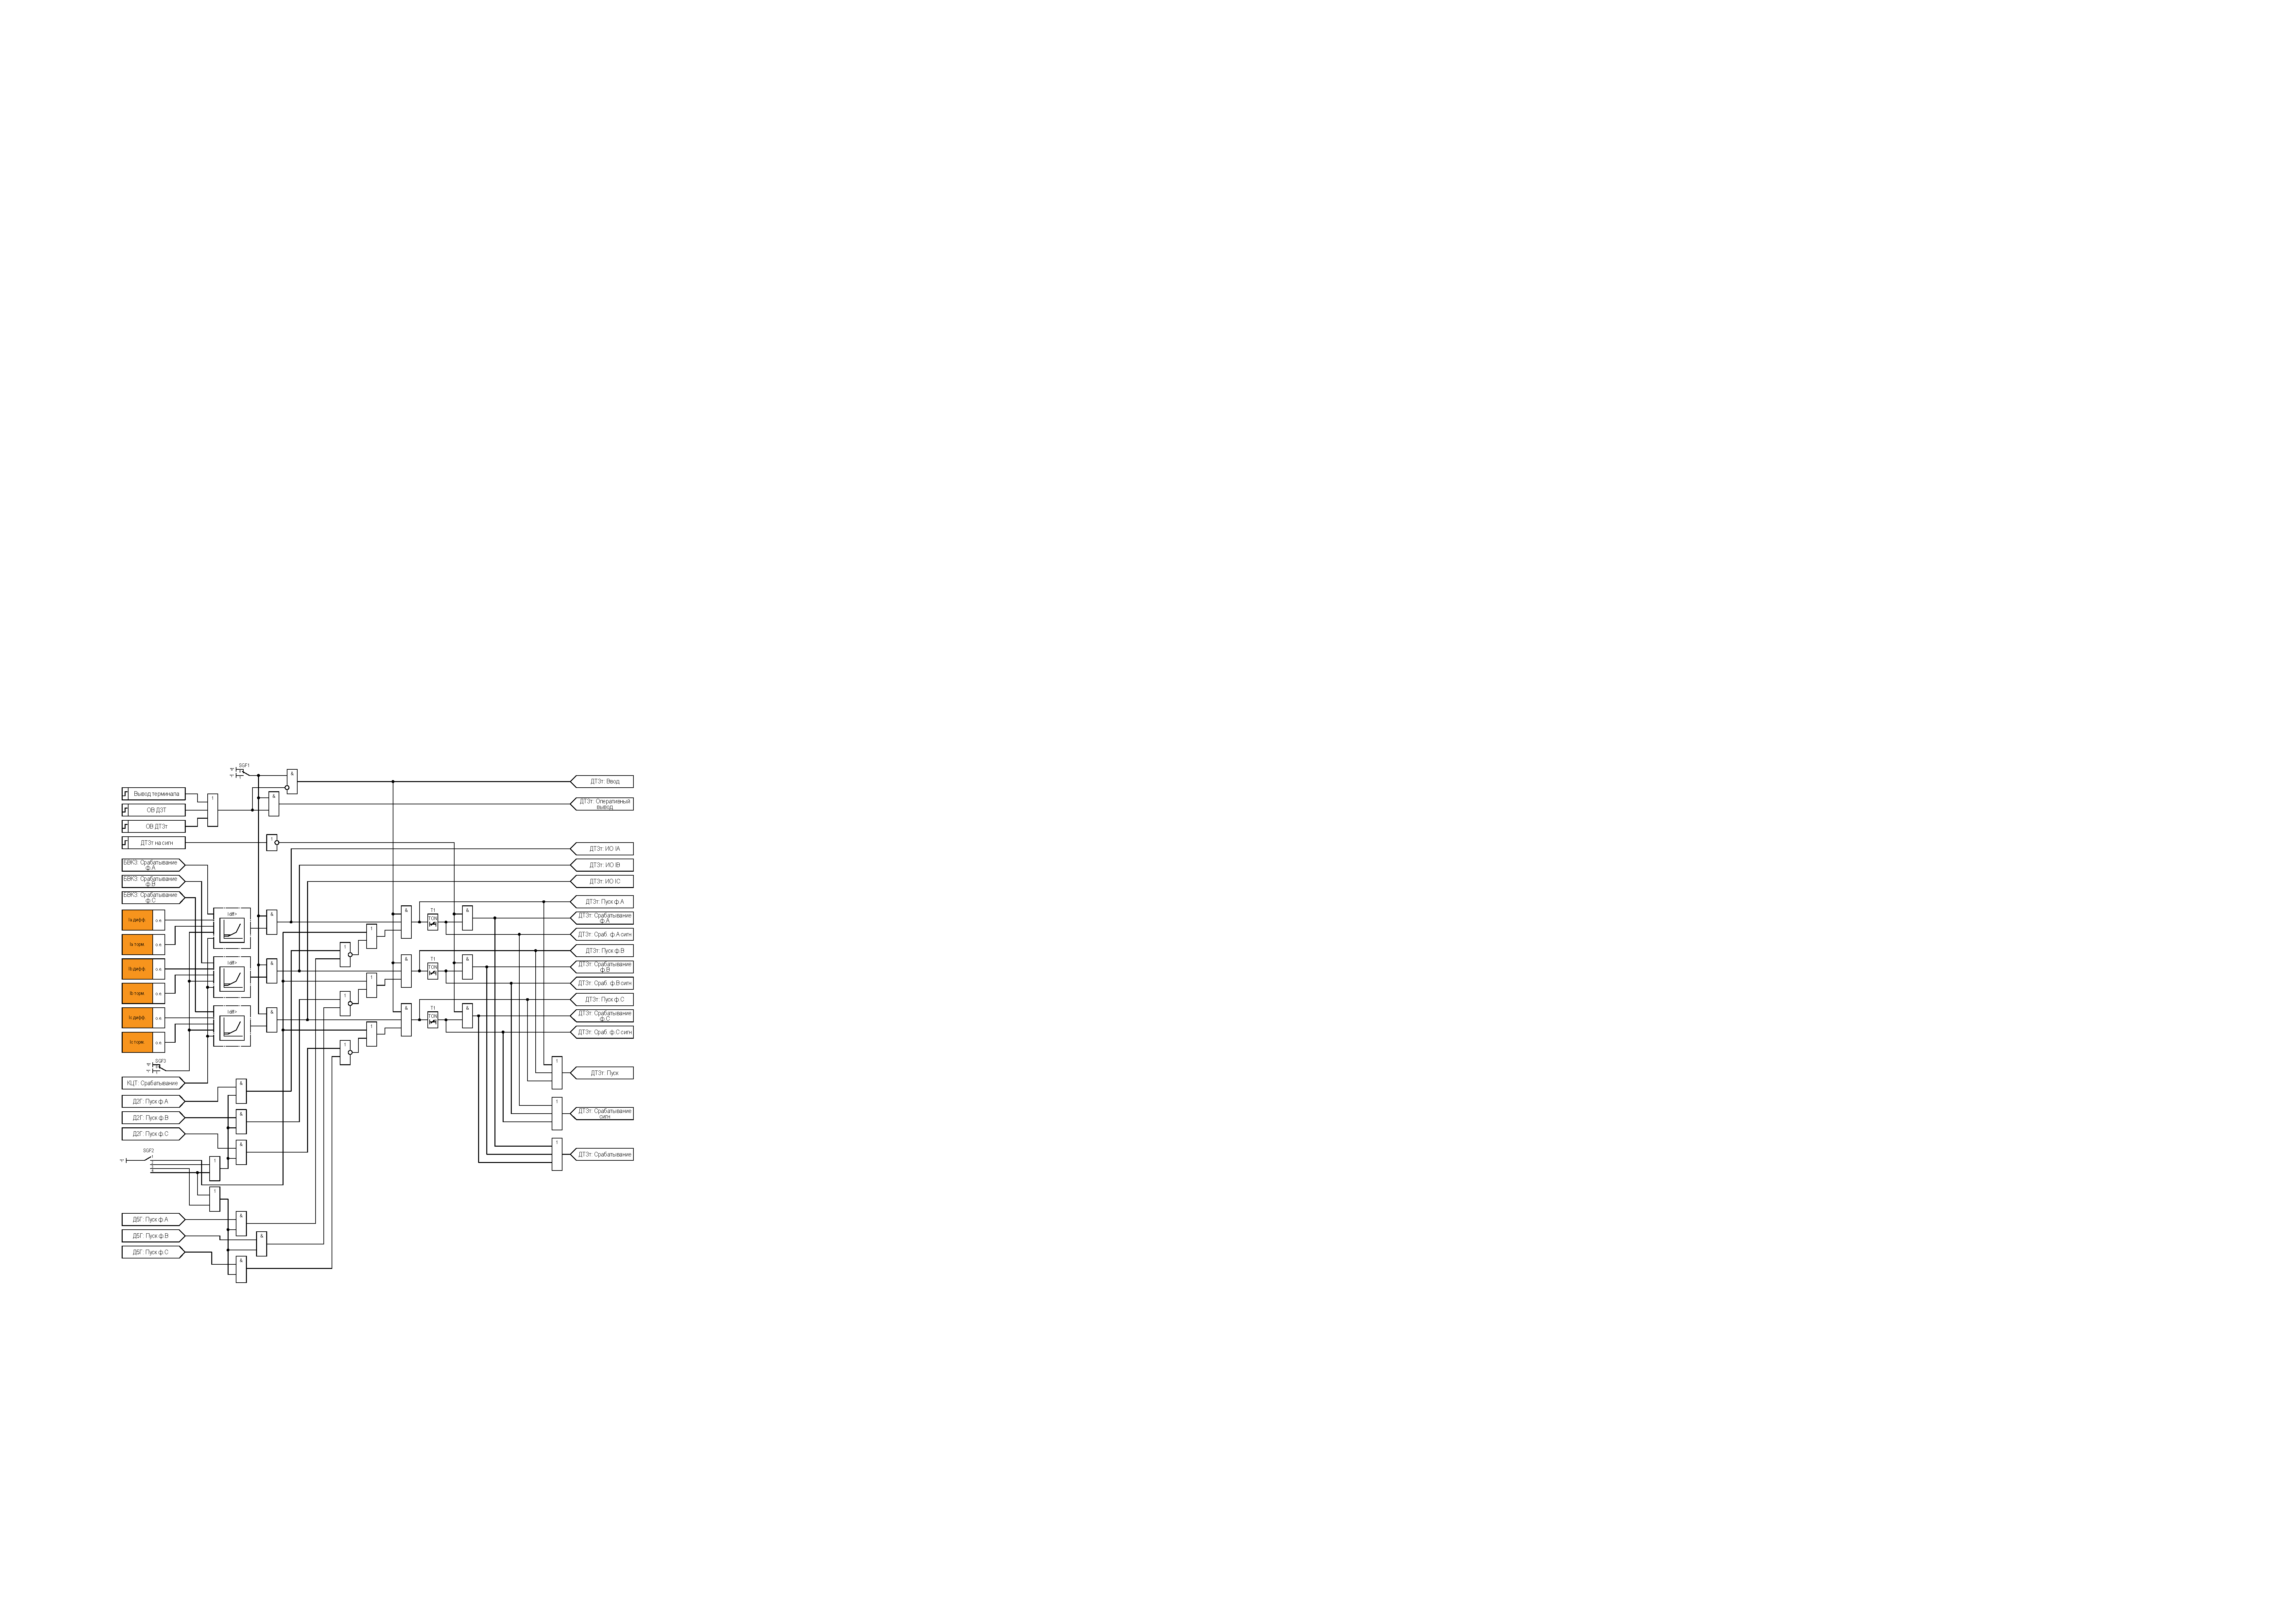
\includegraphics[width=1\textwidth,height=1\textheight,keepaspectratio]{img5.pdf}
\captionof{figure}{Функциональная схема <<ДТЗт>>}
\label{dzt:img1}
\end{figure}
\small
\begin{longtable}{|>{\centering\arraybackslash}m{5.3cm}|>{\centering\arraybackslash}m{3.3cm}|>{\centering\arraybackslash}m{4.2cm}|>{\centering\arraybackslash}m{1.8cm}|>{\centering\arraybackslash}m{1cm}|}
\caption{Параметры для настройки функции <<ДТЗт>>\hfill\vspace{-0.5\baselineskip}}\label{dzt:tbl1}\\ 
\hline
\rowcolor{gray!30}
Параметр (Параметр на ИЧМ) & Условное обозначение на схеме & Значение/ Диапазон & Единица измерения & Шаг \\ 
\hline
\endfirsthead
\caption*{\hspace{3pt}\emph{Продолжение таблицы \ref{dzt:tbl1}\hfill\vspace{-0.5\baselineskip}}} \\ % сделано по ГОСТ 2.105 п.6.8.7
\hline
\rowcolor{gray!30}
Параметр (Параметр на ИЧМ) & Условное обозначение на схеме & Значение/ Диапазон & Единица измерения & Шаг \\ 
\endhead
\endfoot
\endlastfoot
\centering Ввод функции в работу (Ввод\_функции) & \centering SGF1 & \centering 0 = Не предусмотрено\\1 = Предусмотрено & \centering -- & \centering \arraybackslash -- \\
\hline
\centering Контроль от БВКЗ (Контр\_БВКЗ) & \centering SGF3 & \centering 0 = Без контроля БВКЗ\\1 = С контролем БВКЗ & \centering -- & \centering \arraybackslash -- \\
\hline
\centering Режим блокировки (Реж\_блок) & \centering SGF2 & \centering 1 = Без блокировки\\2 = Блокировка по 2 гармонике\\3 = Блокировка по 5 гармонике\\4 = Блокировка по 2 и 5 гармоникам & \centering -- & \centering \arraybackslash -- \\
\hline
\centering Начальный дифференциальный ток срабатывания (Iср) & \centering -- & \centering 0,20 ... 0,60 & \centering о.е. & \centering \arraybackslash 0,01 \\
\hline
\centering Начальный дифференциальный ток срабатывания в режиме загрубления (при неисправностях в токовых цепях) (Iср\_загр) & \centering -- & \centering 0,20 ... 10,00 & \centering о.е. & \centering \arraybackslash 0,01 \\
\hline
\centering Коэффициент торможения первого наклонного участка (Kт1) & \centering -- & \centering 0,20 ... 1,00 & \centering о.е. & \centering \arraybackslash 0,01 \\
\hline
\centering Начальный тормозной ток первого наклонного участка (Iт1) & \centering -- & \centering 0,60 ... 3,00 & \centering о.е. & \centering \arraybackslash 0,01 \\
\hline
\centering Коэффициент торможения второго наклонного участка (Kт2) & \centering -- & \centering 0,20 ... 1,00 & \centering о.е. & \centering \arraybackslash 0,01 \\
\hline
\centering Начальный тормозной ток второго наклонного участка (Iт2) & \centering -- & \centering 1,20 ... 10,00 & \centering о.е. & \centering \arraybackslash 0,01 \\
\hline
\centering Выдержка времени срабатывания (Tср) & \centering T1 & \centering 0,00 ... 3,00 & \centering с & \centering \arraybackslash 0,01 \\
\hline
\end{longtable}
\normalsize

\end{enumerate}

\item Дифференциальная токовая отсечка (ДТО)

\begin{enumerate}[label=\arabic{section}.\arabic{subsection}.\arabic{enumi}.\arabic*, labelsep=4pt, leftmargin=0em, itemindent=65pt, parsep=0pt]

\item
Функция дифференциальной токовой отсечки (<<ДТО>>) предназначена для быстрого и селективного отключения повреждений, сопровождающихся большими токами КЗ в зоне действия ДЗТ. Характеристика срабатывания <<ДТО>> (см. рисунок \ref{dzt:char}) представляет из себя прямую линию, определяемую уставкой <<Iср>>. Функция <<ДТО>> работает без каких-либо блокировок и не имеет торможения. Срабатывание функции <<ДТО>> происходит, если дифференциальный ток превышает уставку <<Iср>> в течении выдержки времени <<Тср>>. Возврат функции <<ДТО>> происходит, если дифференциальный ток ниже уставки <<Iср>> с учетом коэффициента возврата (<<Kвоз>> равен 0,95).

\item
Ввод <<ДТО>> в работу на этапе параметрирования устройства осуществляется программным переключателем SGF1 <<Ввод\_функции>>. Информация о введенной функции отображается выходным сигналом <<ДТО: Ввод>>.
\item
Функция <<ДТО>> может быть выведена из работы оперативно путем активации сигнала <<ОВ ДТО>>, что характеризуется активным состоянием сигнала <<ДТО: Оперативный вывод>> на выходе функции. 
\item
При активном состоянии входного сигнала <<ДТО~на~сигн>> действие отключающей логики переводится на сигнал.
\item
Алгоритм работы функции <<ДТО>> выполнен в соответствии с рисунком \ref{dzt:img2}. В таблице \ref{dzt:tbl2} приведены параметры, необходимые для настройки функции <<ДТО>>.

\small
\begin{longtable}{|>{\centering\arraybackslash}m{5.3cm}|>{\centering\arraybackslash}m{3.3cm}|>{\centering\arraybackslash}m{4.2cm}|>{\centering\arraybackslash}m{1.8cm}|>{\centering\arraybackslash}m{1cm}|}
\caption{Параметры для настройки функции <<ДТО>>\hfill\vspace{-0.5\baselineskip}}\label{dzt:tbl2}\\ 
\hline
\rowcolor{gray!30}
Параметр (Параметр на ИЧМ) & Условное обозначение на схеме & Значение/ Диапазон & Единица измерения & Шаг \\ 
\hline
\endfirsthead
\caption*{\hspace{3pt}\emph{Продолжение таблицы \ref{dzt:tbl2}\hfill\vspace{-0.5\baselineskip}}} \\ % сделано по ГОСТ 2.105 п.6.8.7
\hline
\rowcolor{gray!30}
Параметр (Параметр на ИЧМ) & Условное обозначение на схеме & Значение/ Диапазон & Единица измерения & Шаг \\ 
\endhead
\endfoot
\endlastfoot
\centering Ввод функции в работу (Ввод\_функции) & \centering SGF1 & \centering 0 = Не предусмотрено\\1 = Предусмотрено & \centering -- & \centering \arraybackslash -- \\
\hline
\centering Дифференциальный ток срабатывания (Iср) & \centering I$>$ & \centering 3,0 ... 20,0 & \centering о.е. & \centering \arraybackslash 0,1 \\
\hline
\centering Выдержка времени срабатывания (Tср) & \centering T1 & \centering 0,00 ... 3,00 & \centering с & \centering \arraybackslash 0,01 \\
\hline
\end{longtable}
\normalsize

\vspace{1mm}
\begin{figure}[H]
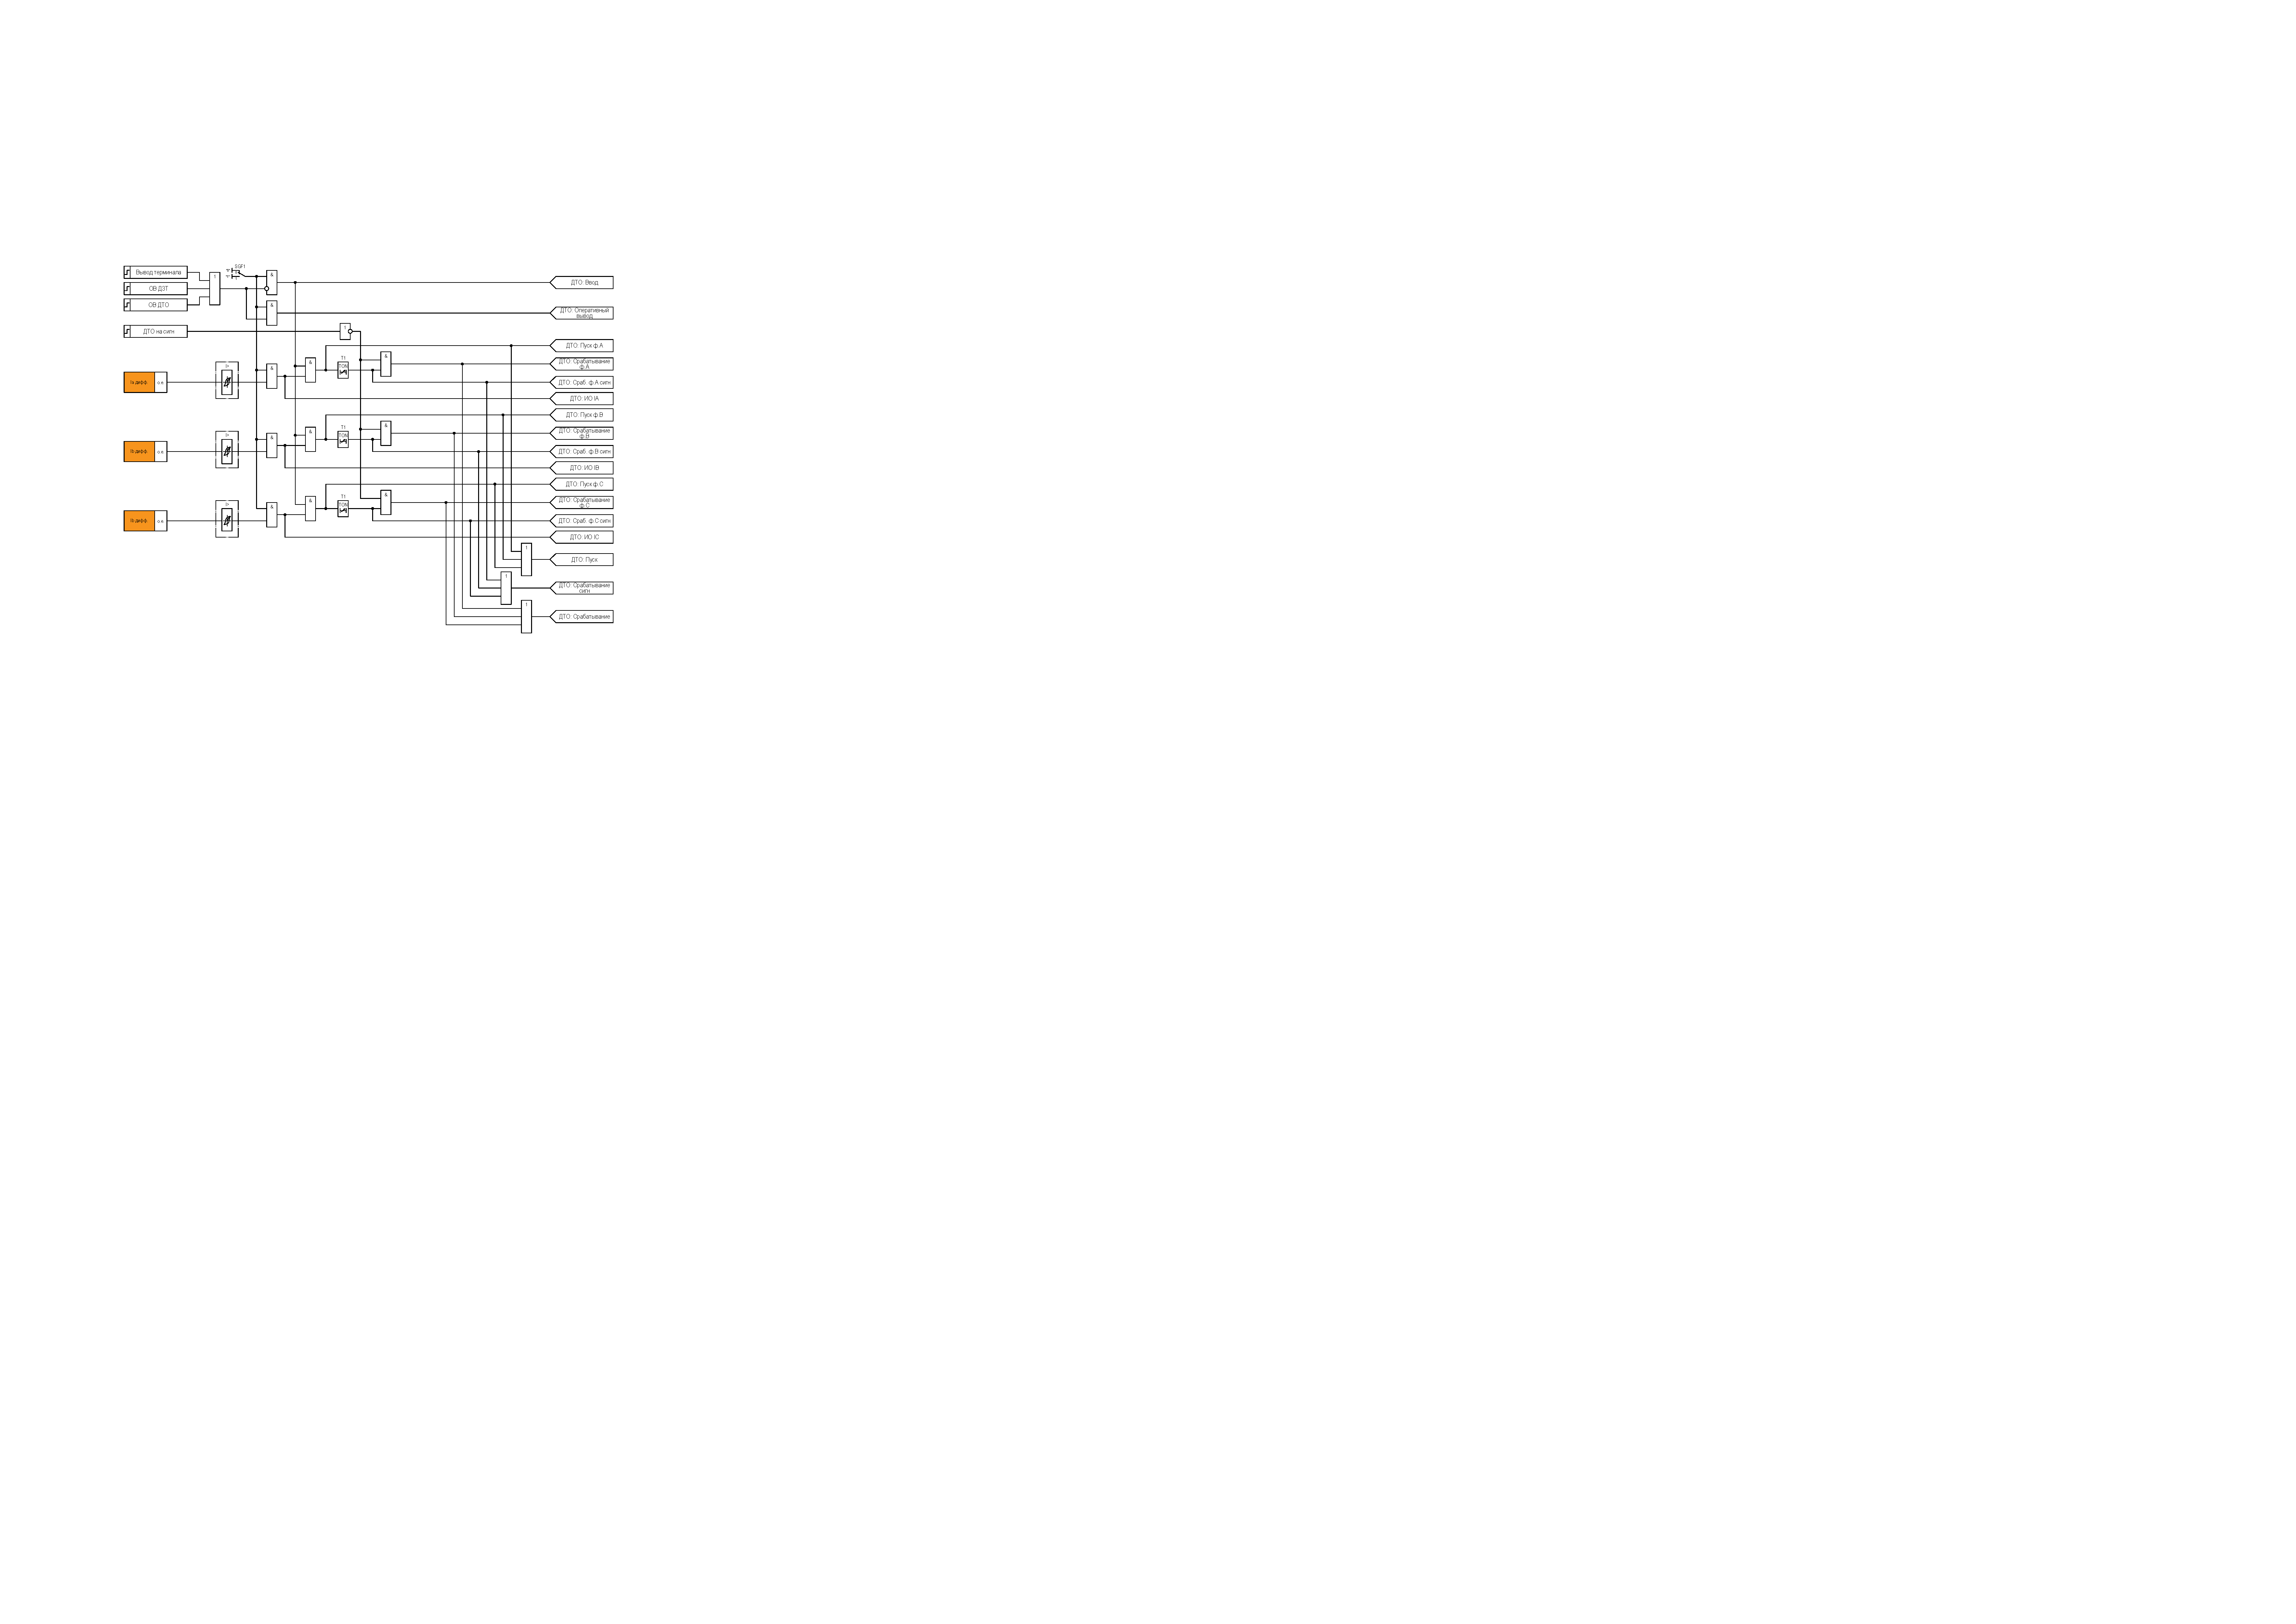
\includegraphics[width=\textwidth,height=\textheight,keepaspectratio]{img6.pdf}
\captionof{figure}{Функциональная схема <<ДТО>>}
\label{dzt:img2}
\end{figure}


\end{enumerate}


\item Детектор второй гармоники (Д2Г)

\begin{enumerate}[label=\arabic{section}.\arabic{subsection}.\arabic{enumi}.\arabic*, labelsep=4pt, leftmargin=0em, itemindent=65pt, parsep=0pt]

\item
Функция детектора второй гармоники (<<Д2Г>>) предусмотрена для отстройки ДЗТ от режимов бросков токов намагничивания, обусловленными остаточным насыщением магнитопровода при включении силового трансформатора. Алгоритм функции <<Д2Г>> контролирует уровень второй гармоники в дифференциальном токе и реагирует на отношение модуля второй гармоники дифференциального тока к модулю основной гармоники. Если данное соотношение превышает уставку <<Ih2/Ih1>> происходит блокировка срабатывания функции <<ДТЗт>>, которая сохраняется до тех пор, пока соотношение не опустится ниже заданной уставки с учетом коэффициента возврата после набора выдержки времени на возврат <<Твоз>>. Срабатывание <<ДТЗт>> блокируется пофазно при появлении соответствующего блокирующего сигнала. 
\item
Ввод функции <<Д2Г>> в работу осуществляется автоматически при выполнении следующих условий:
\begin{itemize}
\item ввод функции <<ДТЗт>> в работу; 
\item\sloppy посредством программного переключателя <<Режим блокировки>> функции <<ДТЗт>> выбран один из режимов: <<Блокировка по 2 гармонике>> или <<Блокировка по 2 и 5 гармоникам>>.
\end{itemize}
\item
Дополнительно, в логике функции <<Д2Г>> должен быть реализован режим перекрестной блокировки (ввод производится уставкой <<Перекр\_блок>>). Принцип работы данного режима заключается в следующем:
\begin{itemize}
\item при обнаружении условий срабатывания <<Д2Г>> в одной из трех фаз должно произойти блокирование срабатывания <<ДТЗт>> по всем трем фазам на время, задаваемое уставкой <<Tперек\_блок>>;
\item при пропадании условий срабатывания <<Д2Г>> от смежных фаз или по истечению времени <<Tперек\_блок>> должно осуществляться блокирование срабатывания <<ДТЗт>> пофазно.
\end{itemize}
\item
Алгоритм работы функции <<Д2Г>> выполнен в соответствии с рисунком \ref{dzt:imgd2g}. В таблице \ref{dzt:tbld2g} приведены параметры, необходимые для настройки функции <<Д2Г>>. 

\vspace{1mm}
\begin{figure}[H]
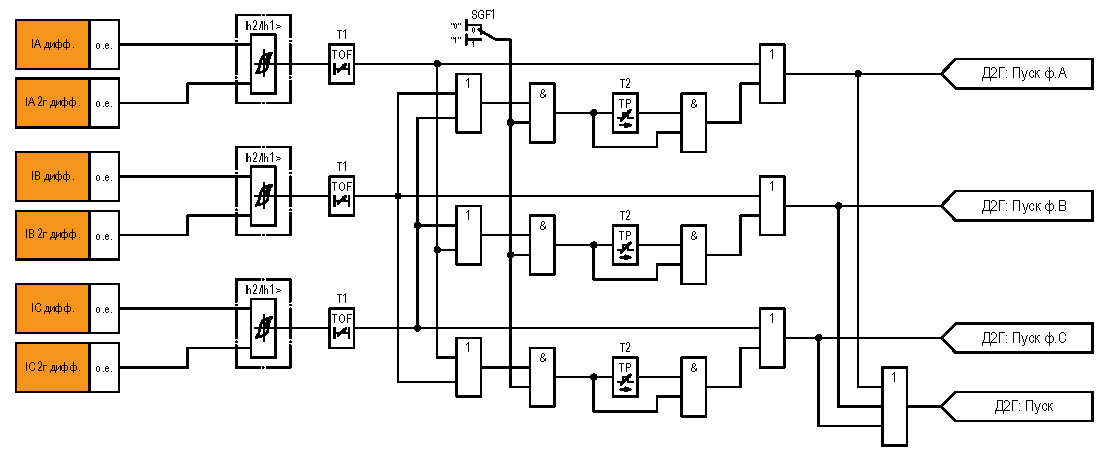
\includegraphics[width=\textwidth,height=\textheight,keepaspectratio]{img7.pdf}
\captionof{figure}{Функциональная схема <<Д2Г>>}
\label{dzt:imgd2g}
\end{figure}
\small
\begin{longtable}{|>{\centering\arraybackslash}m{5.3cm}|>{\centering\arraybackslash}m{3.3cm}|>{\centering\arraybackslash}m{4.2cm}|>{\centering\arraybackslash}m{1.8cm}|>{\centering\arraybackslash}m{1cm}|}
\caption{Параметры для настройки функции <<Д2Г>>\hfill\vspace{-0.5\baselineskip}}\label{dzt:tbld2g}\\ 
\hline
\rowcolor{gray!30}
Параметр (Параметр на ИЧМ) & Условное обозначение на схеме & Значение/ Диапазон & Единица измерения & Шаг \\ 
\hline
\endfirsthead
\caption*{\hspace{3pt}\emph{Продолжение таблицы \ref{dzt:tbld2g}\hfill\vspace{-0.5\baselineskip}}} \\ % сделано по ГОСТ 2.105 п.6.8.7
\hline
\rowcolor{gray!30}
Параметр (Параметр на ИЧМ) & Условное обозначение на схеме & Значение/ Диапазон & Единица измерения & Шаг \\ 
\endhead
\endfoot
\endlastfoot
\centering Коэффициент отношения второй гармоники к первой гармонике для выполнения пусковых условий (Ih2/Ih1) & \centering I2г/I1г$>$ & \centering 0,10 ... 0,50 & \centering -- & \centering \arraybackslash 0,01 \\
\hline
\centering Режим перекрестной блокировки (Перекр\_блок) & \centering SGF1 & \centering 0 = Не предусмотрено\\1 = Предусмотрено & \centering -- & \centering \arraybackslash -- \\
\hline
\centering Выдержка времени ввода перекрестной блокировки (Tперек\_блок) & \centering T2 & \centering 0,06 ... 4,00 & \centering с & \centering \arraybackslash 0,01 \\
\hline
\centering Выдержка времени на возврат (Tвоз) & \centering T1 & \centering 0,000 ... 0,100 & \centering с & \centering \arraybackslash 0,001 \\
\hline
\end{longtable}
\normalsize

\end{enumerate}


\item Детектор пятой гармоники (Д5Г)

\begin{enumerate}[label=\arabic{section}.\arabic{subsection}.\arabic{enumi}.\arabic*, labelsep=4pt, leftmargin=0em, itemindent=65pt, parsep=0pt]

\item
Функция детектора пятой гармоники (<<Д5Г>>) предусмотрена для отстройки ДЗТ от режимов бросков токов намагничивания, обусловленными остаточным насыщением магнитопровода при включении силового трансформатора. Алгоритм функции <<Д5Г>> контролирует уровень второй гармоники в дифференциальном токе и реагирует на отношение модуля второй гармоники дифференциального тока к модулю основной гармоники. Если данное соотношение превышает уставку <<Ih5/Ih1>> происходит блокировка срабатывания функции <<ДТЗт>>, которая сохраняется до тех пор, пока соотношение не опустится ниже заданной уставки с учетом коэффициента возврата после набора выдержки времени на возврат <<Твоз>>. Срабатывание <<ДТЗт>> блокируется пофазно при появлении соответствующего блокирующего сигнала. 
\item
Ввод функции <<Д5Г>> в работу осуществляется автоматически при выполнении следующих условий:
\begin{itemize}
\item ввод функции <<ДТЗт>> в работу; 
\item\sloppy посредством программного переключателя <<Режим блокировки>> функции <<ДТЗт>> выбран один из режимов: <<Блокировка по 5 гармонике>> или <<Блокировка по 2 и 5 гармоникам>>.
\end{itemize}
\item
Дополнительно, в логике функции <<Д5Г>> должен быть реализован режим перекрестной блокировки (ввод производится уставкой <<Перекр\_блок>>). Принцип работы данного режима заключается в следующем:
\begin{itemize}
\item при обнаружении условий срабатывания <<Д5Г>> в одной из трех фаз должно произойти блокирование срабатывания <<ДТЗт>> по всем трем фазам на время, задаваемое уставкой <<Tперек\_блок>>;
\item при пропадании условий срабатывания <<Д5Г>> от смежных фаз или по истечению времени <<Tперек\_блок>> должно осуществляться блокирование срабатывания <<ДТЗт>> пофазно.
\end{itemize}

\item
Алгоритм работы <<Д5Г>> выполнен в соответствии с рисунком \ref{dzt:imgd5g}. В таблице \ref{dzt:tbld5g} приведены параметры, необходимые для настройки функции <<Д5Г>>.

\vspace{1mm}
\begin{figure}[H]
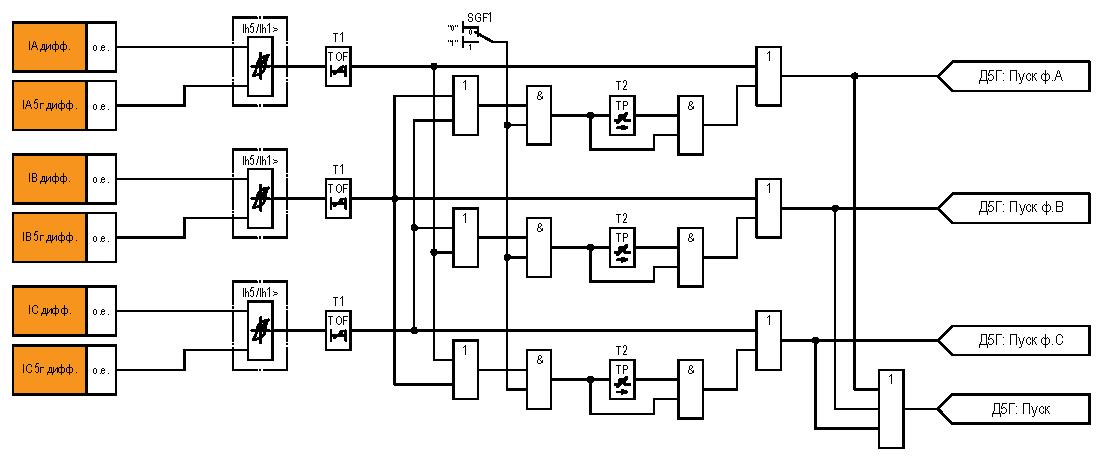
\includegraphics[width=\textwidth,height=\textheight,keepaspectratio]{img8.pdf}
\captionof{figure}{Функциональная схема <<Д5Г>>}
\label{dzt:imgd5g}
\end{figure}
\small
\begin{longtable}{|>{\centering\arraybackslash}m{5.3cm}|>{\centering\arraybackslash}m{3.3cm}|>{\centering\arraybackslash}m{4.2cm}|>{\centering\arraybackslash}m{1.8cm}|>{\centering\arraybackslash}m{1cm}|}
\caption{Параметры для настройки функции <<Д5Г>>\hfill\vspace{-0.5\baselineskip}}\label{dzt:tbld5g}\\ 
\hline
\rowcolor{gray!30}
Параметр (Параметр на ИЧМ) & Условное обозначение на схеме & Значение/ Диапазон & Единица измерения & Шаг \\ 
\hline
\endfirsthead
\caption*{\hspace{3pt}\emph{Продолжение таблицы \ref{dzt:tbld5g}\hfill\vspace{-0.5\baselineskip}}} \\ % сделано по ГОСТ 2.105 п.6.8.7
\hline
\rowcolor{gray!30}
Параметр (Параметр на ИЧМ) & Условное обозначение на схеме & Значение/ Диапазон & Единица измерения & Шаг \\ 
\endhead
\endfoot
\endlastfoot
\centering Коэффициент отношения пятой гармоники к первой гармонике для выполнения пусковых условий (Ih5/Ih1) & \centering I5г/I1г$>$ & \centering 0,05 ... 0,40 & \centering -- & \centering \arraybackslash 0,01 \\
\hline
\centering Режим перекрестной блокировки (Перекр\_блок) & \centering SGF1 & \centering 0 = Не предусмотрено\\1 = Предусмотрено & \centering -- & \centering \arraybackslash -- \\
\hline
\centering Выдержка времени ввода перекрестной блокировки (Tперек\_блок) & \centering T2 & \centering 0,06 ... 4,00 & \centering с & \centering \arraybackslash 0,01 \\
\hline
\centering Выдержка времени на возврат (Tвоз) & \centering T1 & \centering 0,000 ... 0,100 & \centering с & \centering \arraybackslash 0,001 \\
\hline
\end{longtable}
\normalsize

\end{enumerate}


\item\label{sec:bvkz} Блокировка при внешних КЗ (БВКЗ)

\begin{enumerate}[label=\arabic{section}.\arabic{subsection}.\arabic{enumi}.\arabic*, labelsep=4pt, leftmargin=0em, itemindent=65pt, parsep=0pt]

\item
Срабатывание функции блокировки при внешних КЗ (<<БВКЗ>>) является дополнительным критерием стабильной работы ДЗТ при насыщении ТТ. Общий принцип действия состоит в сравнении фаз токов по сторонам защищаемого объекта. Функция <<БВКЗ>> выполняется в пофазном исполнении.
\item
Временные диаграммы работы функции <<БВКЗ>> в режимах внешнего и внутреннего КЗ приведены на рисунке \ref{dzt:imgcharbvkz}, для однозначного соответствия точек измерения на функциональной схеме (рис. \ref{dzt:imgbvkz}) и на временных диаграммах (рис. \ref{dzt:imgcharbvkz}) точкам измерения присвоены цифры \textcircled{\raisebox{-0.9pt}{1}}...\textcircled{\raisebox{-0.9pt}{5}}.
На функциональной схеме (рис. \ref{dzt:imgbvkz}) и временных диаграммах (рис. \ref{dzt:imgcharbvkz}) указаны точки измерений. 

\item
Каждый период выполняется вычисление амплитуд токов сторон. Ток стороны с максимальной амплитудой выбирается в качестве первой величины для сравнения ($i1$). В качестве второй величины для сравнения ($i2$) используется сумма мгновенных значений остальных сторон.

\item
Во время положительной полуволны тока каждой из сравниваемых величин устанавливаются сигналы 1 на определенных элементах схемы. Далее эти сигналы суммируются. При внешних КЗ в сумме сигналов практически отсутствуют паузы (паузы обусловлены пороговыми значениями элементов сравнения). При внутренних КЗ паузы по длительности приближаются к значению времени полупериода (см. рисунок \ref{dzt:imgcharbvkz}). Длительность паузы является критерием блокировки при внешних КЗ. Вторая по счету от начала повреждения длительная пауза дает разрешение на работу ДЗТ.

\vspace{1mm}
\begin{figure}[H]
\centering
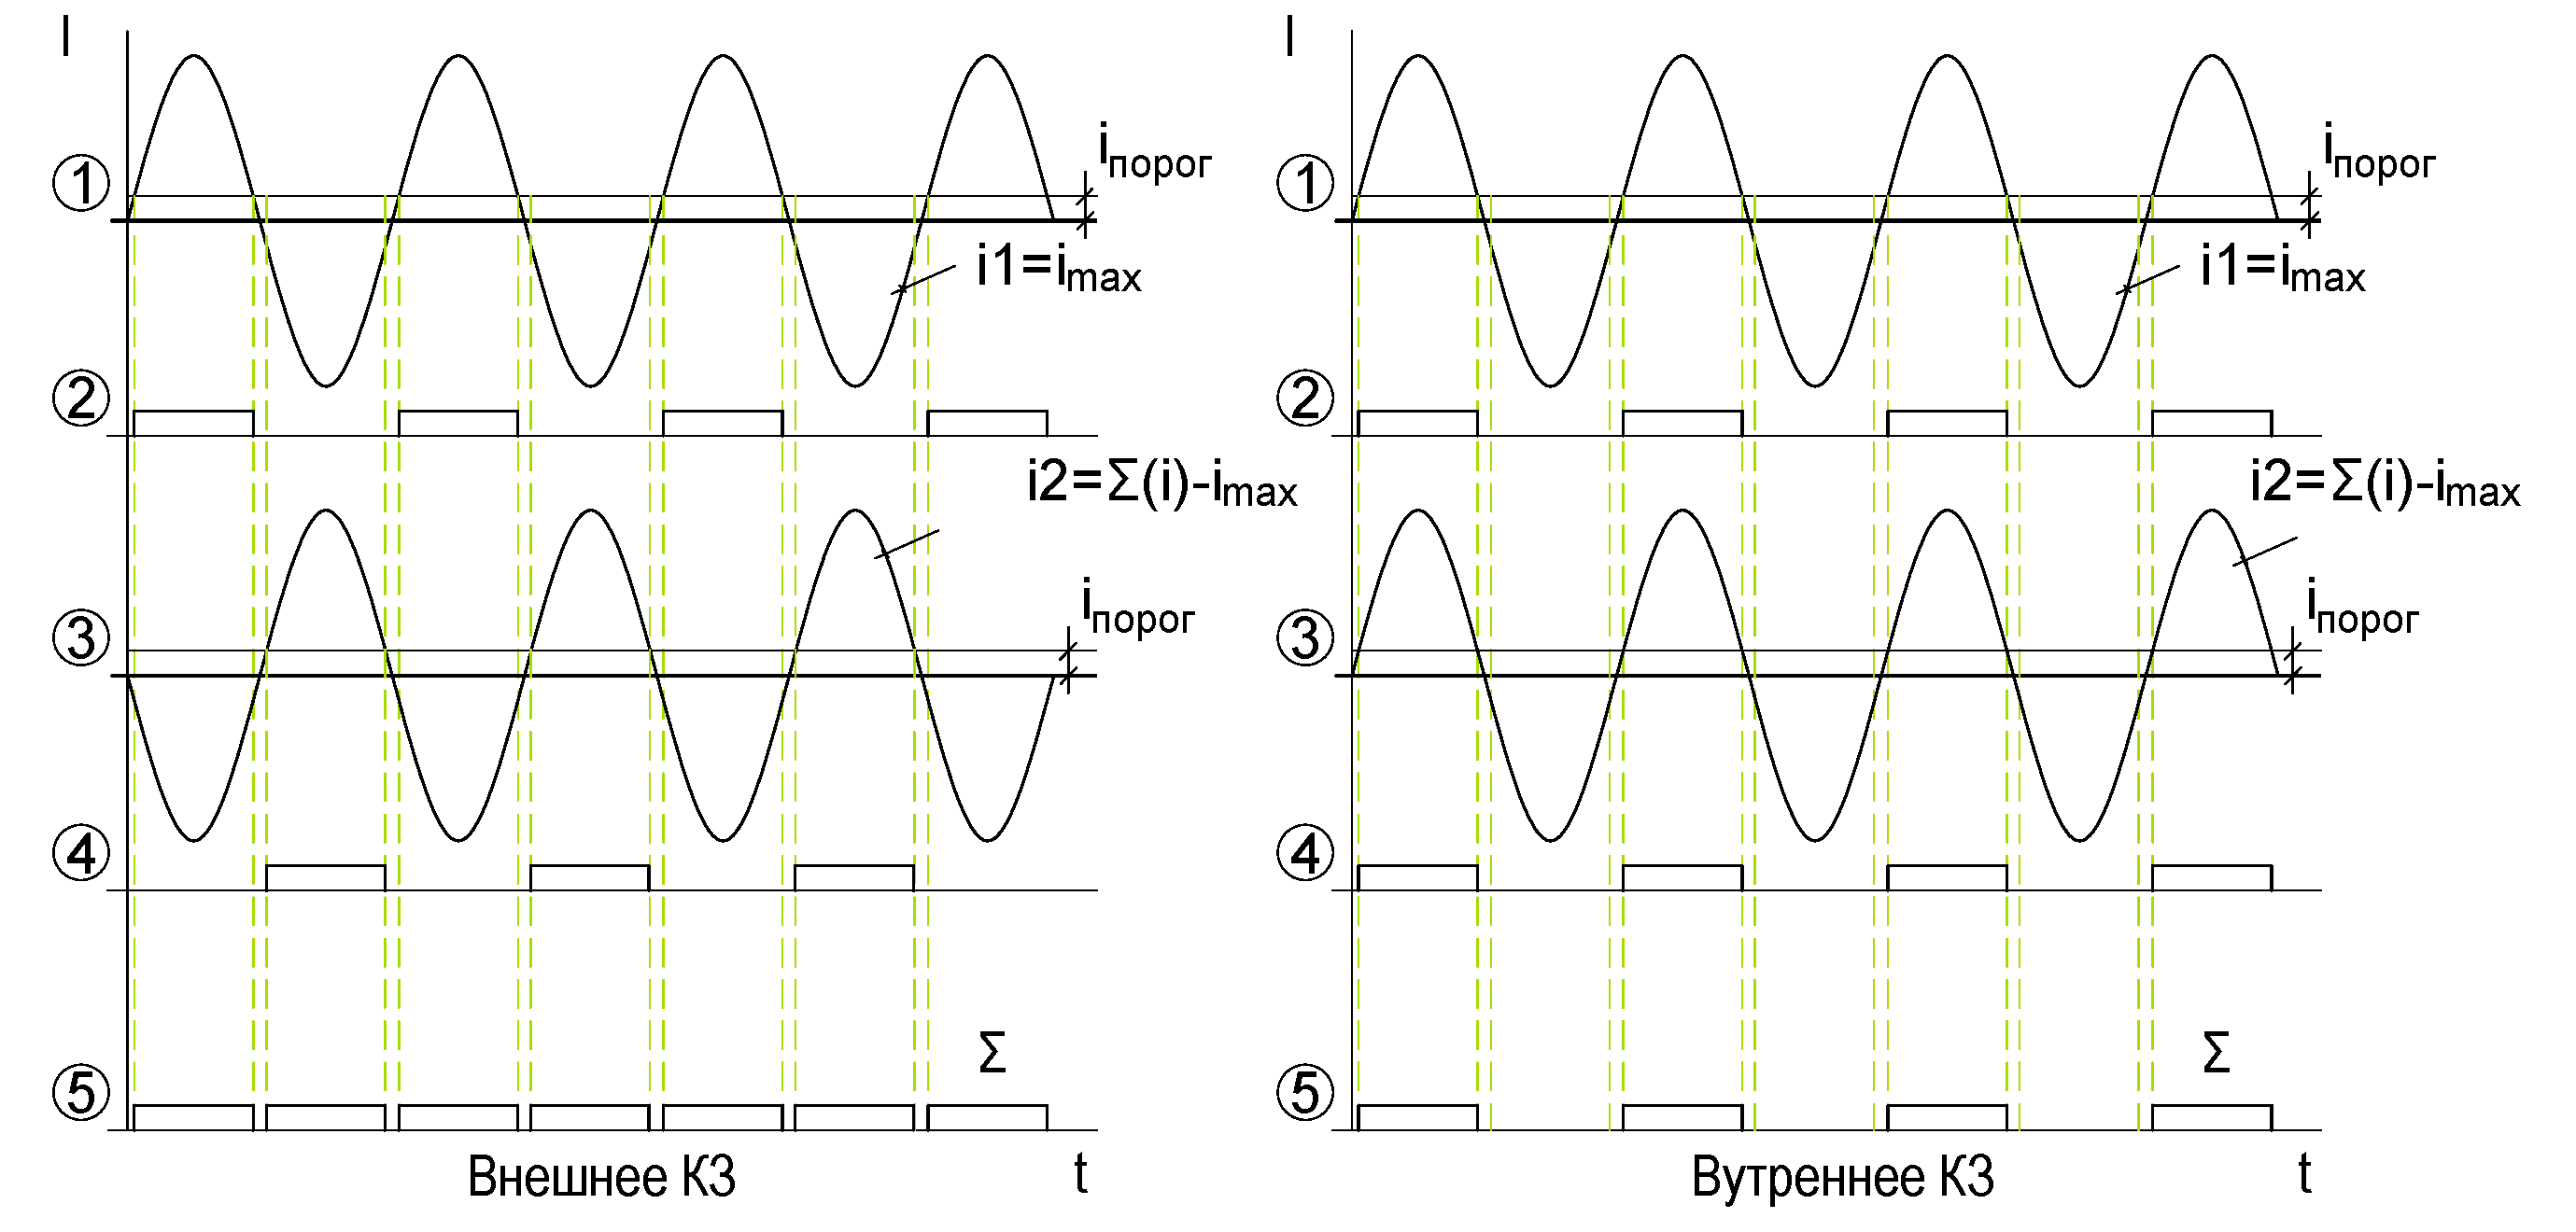
\includegraphics[width=1\textwidth,height=1\textheight,keepaspectratio]{img9.pdf}
\captionof{figure}{Временные диаграммы работы функции <<БВКЗ>>}
\label{dzt:imgcharbvkz}
\end{figure}

\item
Функция <<БВКЗ>> автоматически вводится в работу при введенной в работу функции <<ДТЗт>> и введенном переключателе SGF3 <<Контр\_БВКЗ>> в составе функции <<ДТЗт>>.

\item
Алгоритм работы <<БВКЗ>> выполнен в соответствии с рисунком \ref{dzt:imgbvkz}. Функция <<БВКЗ>> не требует дополнительной настройки.

\vspace{1mm}
\begin{figure}[H]
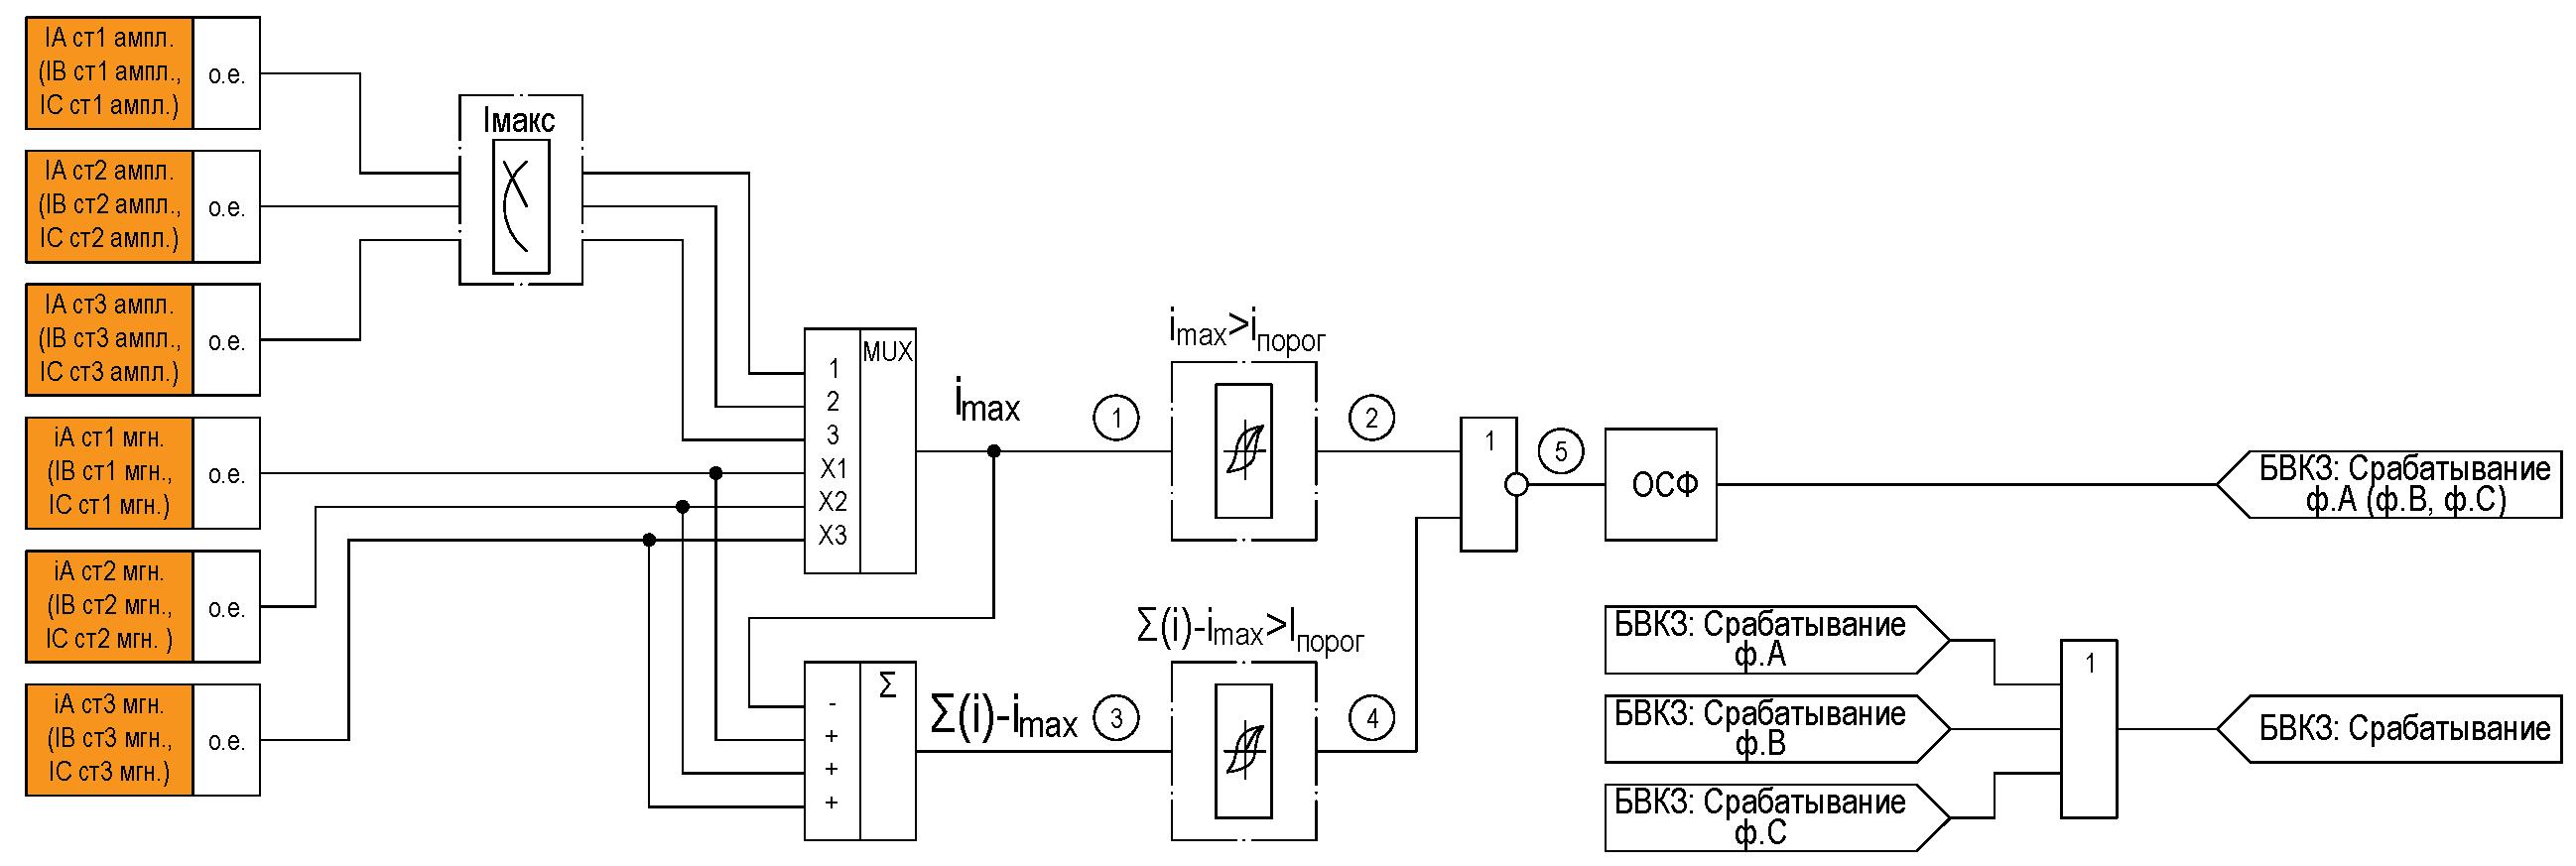
\includegraphics[width=\textwidth,height=\textheight,keepaspectratio]{img10.pdf}
\captionof{figure}{Функциональная схема <<БВКЗ>>}
\label{dzt:imgbvkz}
\end{figure}

\end{enumerate}


\item Контроль исправности токовых цепей по величине небаланса (КЦТнеб)

\begin{enumerate}[label=\arabic{section}.\arabic{subsection}.\arabic{enumi}.\arabic*, labelsep=4pt, leftmargin=0em, itemindent=65pt, parsep=0pt]

\item
Функция контроля исправности токовых цепей по величине небаланса (<<КЦТнеб>>) в дифференциальных цепях является дополнительной. Принцип действия этой функции основан на измерении тока небаланса в дифференциальных цепях: если дифференциальный ток превышает уставку тока небаланса <<Iср>> в течение выдержки времени <<Tср>>, то выдается сигнал о неисправности в сигнализацию.
\item
Ввод функции в работу на этапе параметрирования устройства осуществляется программным переключателем SGF1 <<Ввод\_функции>>. Информация о введенной функции отображается выходным сигналом <<КЦТнеб: Ввод>>.
\item
Функция <<КЦТнеб>> может быть выведена из работы оперативно путем активации сигнала <<ОВ КЦТнеб>>, что характеризуется активным состоянием сигнала <<КЦТнеб: Оперативный вывод>> на выходе функции. 
\item
Алгоритм работы <<КЦТнеб>> выполнен в соответствии с рисунком \ref{dzt:imgkzt}. В таблице \ref{dzt:tblkzt} приведены параметры, необходимые для настройки функции <<КЦТнеб>>.

\vspace{1mm}
\begin{figure}[H]
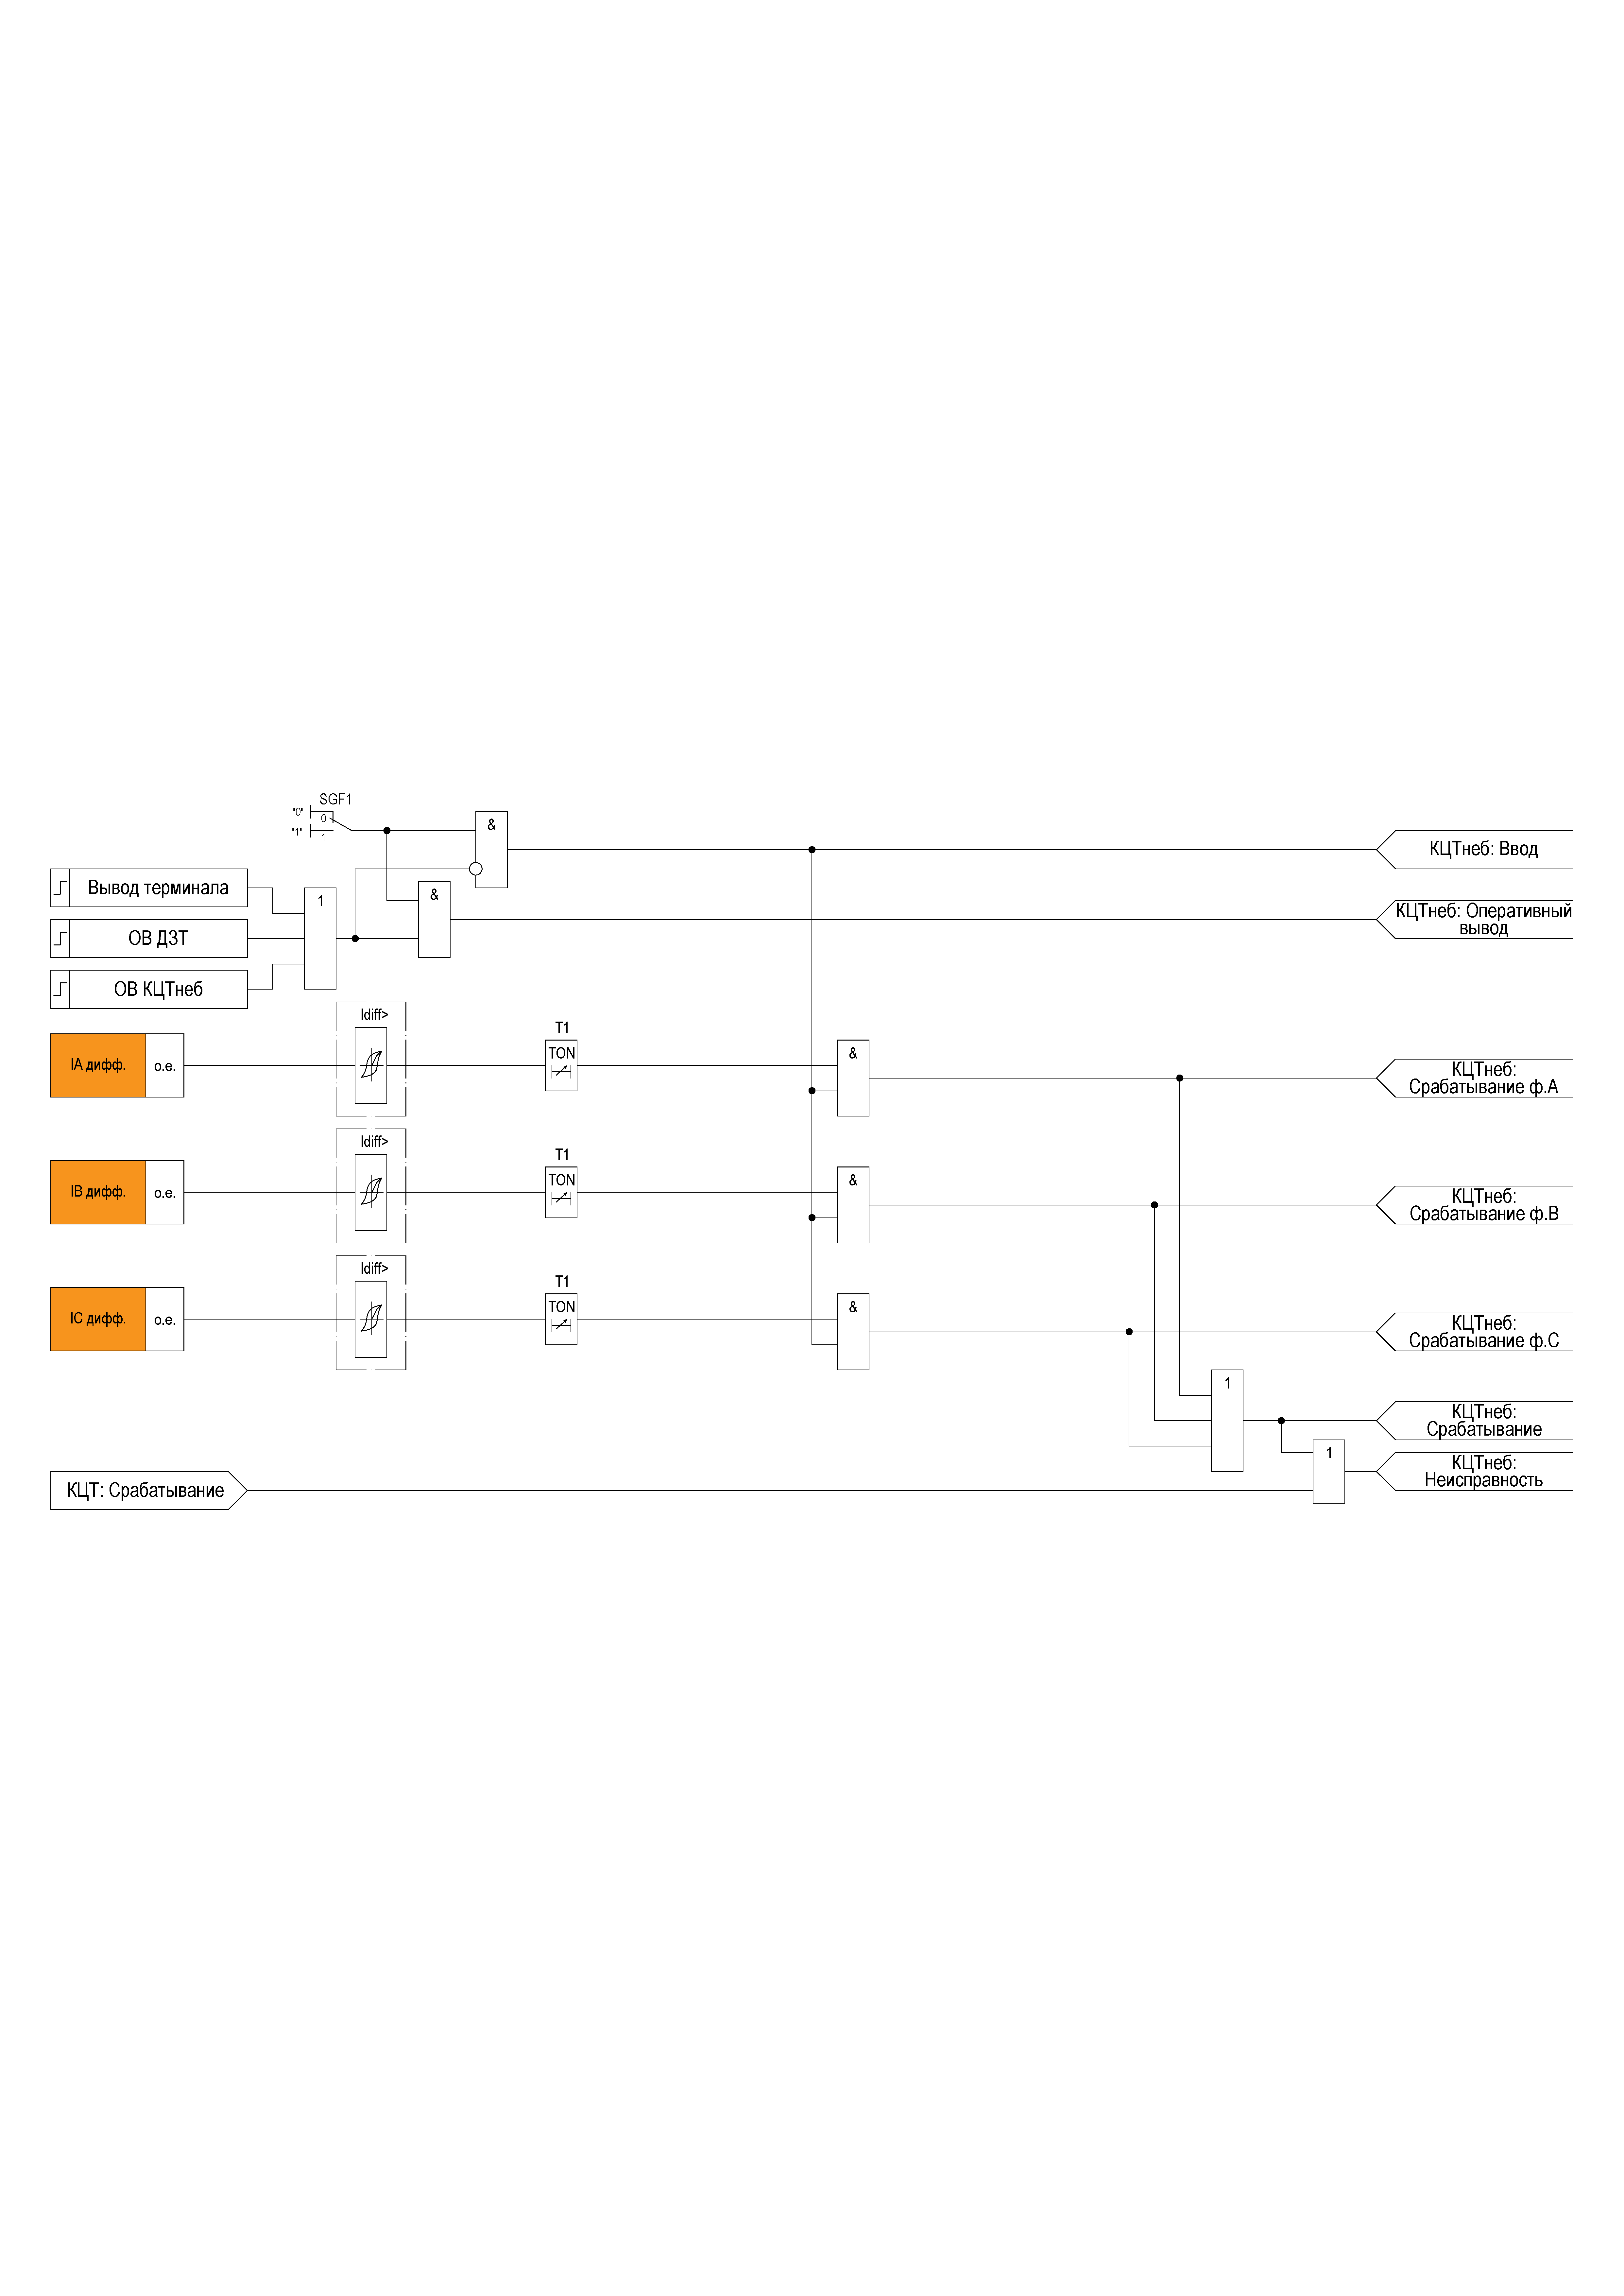
\includegraphics[width=\textwidth,height=\textheight,keepaspectratio]{img11.pdf}
\captionof{figure}{Функциональная схема <<КЦТнеб>>}
\label{dzt:imgkzt}
\end{figure}
\small
\begin{longtable}{|>{\centering\arraybackslash}m{5.3cm}|>{\centering\arraybackslash}m{3.3cm}|>{\centering\arraybackslash}m{4.2cm}|>{\centering\arraybackslash}m{1.8cm}|>{\centering\arraybackslash}m{1cm}|}
\caption{Параметры для настройки функции <<КЦТнеб>>\hfill\vspace{-0.5\baselineskip}}\label{dzt:tblkzt}\\ 
\hline
\rowcolor{gray!30}
Параметр (Параметр на ИЧМ) & Условное обозначение на схеме & Значение/ Диапазон & Единица измерения & Шаг \\ 
\hline
\endfirsthead
\caption*{\hspace{3pt}\emph{Продолжение таблицы \ref{dzt:tblkzt}\hfill\vspace{-0.5\baselineskip}}} \\ % сделано по ГОСТ 2.105 п.6.8.7
\hline
\rowcolor{gray!30}
Параметр (Параметр на ИЧМ) & Условное обозначение на схеме & Значение/ Диапазон & Единица измерения & Шаг \\ 
\endhead
\endfoot
\endlastfoot
\centering Ввод функции в работу (Ввод\_функции) & \centering SGF1 & \centering 0 = Не предусмотрено\\1 = Предусмотрено & \centering -- & \centering \arraybackslash -- \\
\hline
\centering Ток срабатывания (Iср) & \centering Idiff$>$ & \centering 0,04 ... 2,00 & \centering о.е. & \centering \arraybackslash 0,01 \\
\hline
\centering Выдержка времени срабатывания (Tср) & \centering T1 & \centering 0,0 ... 110,0 & \centering с & \centering \arraybackslash 0,1 \\
\hline
\end{longtable}
\normalsize
\end{enumerate}

\item Общие параметры 

\begin{enumerate}[label=\arabic{section}.\arabic{subsection}.\arabic{enumi}.\arabic*, labelsep=4pt, leftmargin=0em, itemindent=65pt, parsep=0pt]

\item
Для правильной работы ДЗТ необходимо задать общие параметры (базисная мощность трансформатора, схема соединения ТТ для каждой из сторон, выбор сторон для расчета дифференциального и тормозного тока). 
В таблице \ref{dzt:tblgen} приведены общие параметры, необходимые для настройки функционального блока <<ДЗТ>>.

\small
\begin{longtable}{|>{\centering\arraybackslash}m{5.3cm}|>{\centering\arraybackslash}m{3.3cm}|>{\centering\arraybackslash}m{4.2cm}|>{\centering\arraybackslash}m{1.8cm}|>{\centering\arraybackslash}m{1cm}|}
\caption{Общие параметры для настройки функционального блока <<ДЗТ>>\hfill\vspace{-0.5\baselineskip}}\label{dzt:tblgen}\\ 
\hline
\rowcolor{gray!30}
Параметр (Параметр на ИЧМ) & Условное обозначение на схеме & Значение/ Диапазон & Единица измерения & Шаг \\ 
\hline
\endfirsthead
\caption*{\hspace{3pt}\emph{Продолжение таблицы \ref{dzt:tblgen}\hfill\vspace{-0.5\baselineskip}}} \\ % сделано по ГОСТ 2.105 п.6.8.7
\hline
\rowcolor{gray!30}
Параметр (Параметр на ИЧМ) & Условное обозначение на схеме & Значение/ Диапазон & Единица измерения & Шаг \\ 
\endhead
\endfoot
\endlastfoot
\centering Сторона 1 (Сторона 1) & \centering -- & \centering 0 = Не используется\\1 = Используется & \centering -- & \centering \arraybackslash -- \\
\hline
\centering Сторона 2 (Сторона 2) & \centering -- & \centering 0 = Не используется\\1 = Используется & \centering -- & \centering \arraybackslash -- \\
\hline
\centering Сторона 3 (Сторона 3) & \centering -- & \centering 0 = Не используется\\1 = Используется & \centering -- & \centering \arraybackslash -- \\
\hline
\centering Схема соединения трансформаторов тока стороны 1 (KсхемСт1) & \centering -- & \centering 0 = Звезда\\1 = Треугольник & \centering -- & \centering \arraybackslash -- \\
\hline
\centering Схема соединения трансформаторов тока стороны 2 (KсхемСт2) & \centering -- & \centering 0 = Звезда\\1 = Треугольник & \centering -- & \centering \arraybackslash -- \\
\hline
\centering Схема соединения трансформаторов тока стороны 3 (KсхемСт3) & \centering -- & \centering 0 = Звезда\\1 = Треугольник & \centering -- & \centering \arraybackslash -- \\
\hline
\centering Базисная мощность (Sbase) & \centering -- & \centering 1,0 ... 500,0 & \centering МВ×А & \centering \arraybackslash 0,1 \\
\hline
\end{longtable}
\normalsize
\end{enumerate}

\item Параметры настройки сторон 

\begin{enumerate}[label=\arabic{section}.\arabic{subsection}.\arabic{enumi}.\arabic*, labelsep=4pt, leftmargin=0em, itemindent=65pt, parsep=0pt]

\item
Для корректного приведения токов сторон силового трансформатора необходимо задать параметры каждой стороны (номинальное напряжение стороны, номинальный первичный ток ТТ стороны, номинальный вторичный ток ТТ стороны, требуется ли компенсация токов нулевой последовательности и номер векторной группы). 
В таблице \ref{dzt:tblside} приведены параметры, необходимые для корректного приведения токов сторон защищаемого трансформатора.

\small
\begin{longtable}{|>{\centering\arraybackslash}m{5.3cm}|>{\centering\arraybackslash}m{3.3cm}|>{\centering\arraybackslash}m{4.2cm}|>{\centering\arraybackslash}m{1.8cm}|>{\centering\arraybackslash}m{1cm}|}
\caption{Параметры, необходимые для корректного приведения токов сторон\hfill\vspace{-0.5\baselineskip}}\label{dzt:tblside}\\ 
\hline
\rowcolor{gray!30}
Параметр (Параметр на ИЧМ) & Условное обозначение на схеме & Значение/ Диапазон & Единица измерения & Шаг \\ 
\hline
\endfirsthead
\caption*{\hspace{3pt}\emph{Продолжение таблицы \ref{dzt:tblside}\hfill\vspace{-0.5\baselineskip}}} \\ % сделано по ГОСТ 2.105 п.6.8.7
\hline
\rowcolor{gray!30}
Параметр (Параметр на ИЧМ) & Условное обозначение на схеме & Значение/ Диапазон & Единица измерения & Шаг \\ 
\endhead
\endfoot
\endlastfoot
\multicolumn{5}{|c|}{ Сторона 1 } \\ \hline 
\centering Номинальное напряжение стороны 1 (Uном1) & \centering -- & \centering 6,0 ... 250,0 & \centering кВ & \centering \arraybackslash 0,1 \\
\hline
\centering Номинальный первичный ток трансформатора тока стороны 1 (IпервСт1) & \centering -- & \centering 1 ... 40000 & \centering А & \centering \arraybackslash 1 \\
\hline
\centering Номинальный вторичный ток трансформатора тока стороны 1 (IвторСт1) & \centering -- & \centering 0,2 ... 5,0 & \centering А & \centering \arraybackslash 0,1 \\
\hline
\centering Компенсация токов 3I0 для стороны 1 (Компенс3I0ст1) & \centering -- & \centering 0 = Без компенсации токов 3I0\\1 = С компенсацией токов 3I0 & \centering -- & \centering \arraybackslash -- \\
\hline
\centering Векторная группа стороны 1 (Nсх1) & \centering -- & \centering 0 ... 11 & \centering -- & \centering \arraybackslash 1 \\
\hline
\multicolumn{5}{|c|}{ Сторона 2 } \\ \hline 
\centering Номинальное напряжение стороны 2 (Uном2) & \centering -- & \centering 6,0 ... 250,0 & \centering кВ & \centering \arraybackslash 0,1 \\
\hline
\centering Номинальный первичный ток трансформатора тока стороны 2 (IпервСт2) & \centering -- & \centering 1 ... 40000 & \centering А & \centering \arraybackslash 1 \\
\hline
\centering Номинальный вторичный ток трансформатора тока стороны 2 (IвторСт2) & \centering -- & \centering 0,2 ... 5,0 & \centering А & \centering \arraybackslash 0,1 \\
\hline
\centering Компенсация токов 3I0 для стороны 2 (Компенс3I0ст2) & \centering -- & \centering 0 = Без компенсации токов 3I0\\1 = С компенсацией токов 3I0 & \centering -- & \centering \arraybackslash -- \\
\hline
\centering Векторная группа стороны 2 (Nсх2) & \centering -- & \centering 0 ... 11 & \centering -- & \centering \arraybackslash 1 \\
\hline
\multicolumn{5}{|c|}{ Сторона 3 } \\ \hline 
\centering Номинальное напряжение стороны 3 (Uном3) & \centering -- & \centering 6,0 ... 250,0 & \centering кВ & \centering \arraybackslash 0,1 \\
\hline
\centering Номинальный первичный ток трансформатора тока стороны 3 (IпервСт3) & \centering -- & \centering 1 ... 40000 & \centering А & \centering \arraybackslash 1 \\
\hline
\centering Номинальный вторичный ток трансформатора тока стороны 3 (IвторСт3) & \centering -- & \centering 0,2 ... 5,0 & \centering А & \centering \arraybackslash 0,1 \\
\hline
\centering Компенсация токов 3I0 для стороны 3 (Компенс3I0ст3) & \centering -- & \centering 0 = Без компенсации токов 3I0\\1 = С компенсацией токов 3I0 & \centering -- & \centering \arraybackslash -- \\
\hline
\centering Векторная группа стороны 3 (Nсх3) & \centering -- & \centering 0 ... 11 & \centering -- & \centering \arraybackslash 1 \\
\hline
\end{longtable}
\normalsize
\end{enumerate}

\end{enumerate}
\needspace{4\baselineskip}
\color{uniblue}{\subsection{Контроль токовых цепей (КЦТ)}\label{sec:kzt}}
\color{black}

\begin{enumerate}[label=\arabic{section}.\arabic{subsection}.\arabic*, labelsep=4pt, leftmargin=0pt, itemindent=57pt]

\item
Функциональный блок <<КЦТ>> предназначен для контроля токовых цепей, подключенных к аналоговым входам микропроцессорного устройства защиты. В состав функционального блока входят функции контроля токовых цепей по сторонам трансформатора (<<КЦТ ВН>>, <<КЦТ НН1>>, <<КЦТ НН2>>). Сигнал неисправности токовых цепей формируется логическим суммированием сигналов нарушения симметрии от каждой из функций контроля токовых цепей сторон трансформатора. При фиксации неисправности токовых цепей формируется сигнал <<КЦТ: Срабатывание>>, который заводится в функцию <<ДТЗт>> (см. пункт \ref{sec:dtzt}). 
\item
Функциональный блок <<КЦТ>> может быть выведен из работы оперативно путем активации сигнала <<ОВ КЦТ>>, при этом осуществляется вывод функций контроля токовых цепей каждой из сторон силового трансформатора (ВН, НН1, НН2).
\item
Ввод функции контроля токовых цепей каждой стороны в работу на этапе параметрирования устройства осуществляется своим программным переключателем SGF1 <<Ввод\_функции>>. Информация о введенной функции отображается выходным сигналом для каждой функции (<<КЦТ ВН: Ввод>>, <<КЦТ НН1: Ввод>>, <<КЦТ НН2: Ввод>>).
\item
Функция контроля токовых цепей любой стороны силового трансформатора (ВН, НН1, НН2) <<КЦТ ВН (НН1, НН2)>> может быть выведена из работы оперативно путем активации сигнала <<ОВ КЦТ ВН>>, <<ОВ КЦТ НН1>> или <<ОВ КЦТ НН2>> соответственно, при этом активизируется выходной сигнал <<Оперативный вывод>> для соответствующих функций.
\item
Алгоритм работы <<КЦТ>> выполнен в соответствии с рисунком \ref{kzt:img1}. В таблице \ref{kzt:tbl1} приведены параметры, необходимые для настройки функции <<КЦТ>>.

\vspace{3mm}
\begin{figure}[!h]
\centering
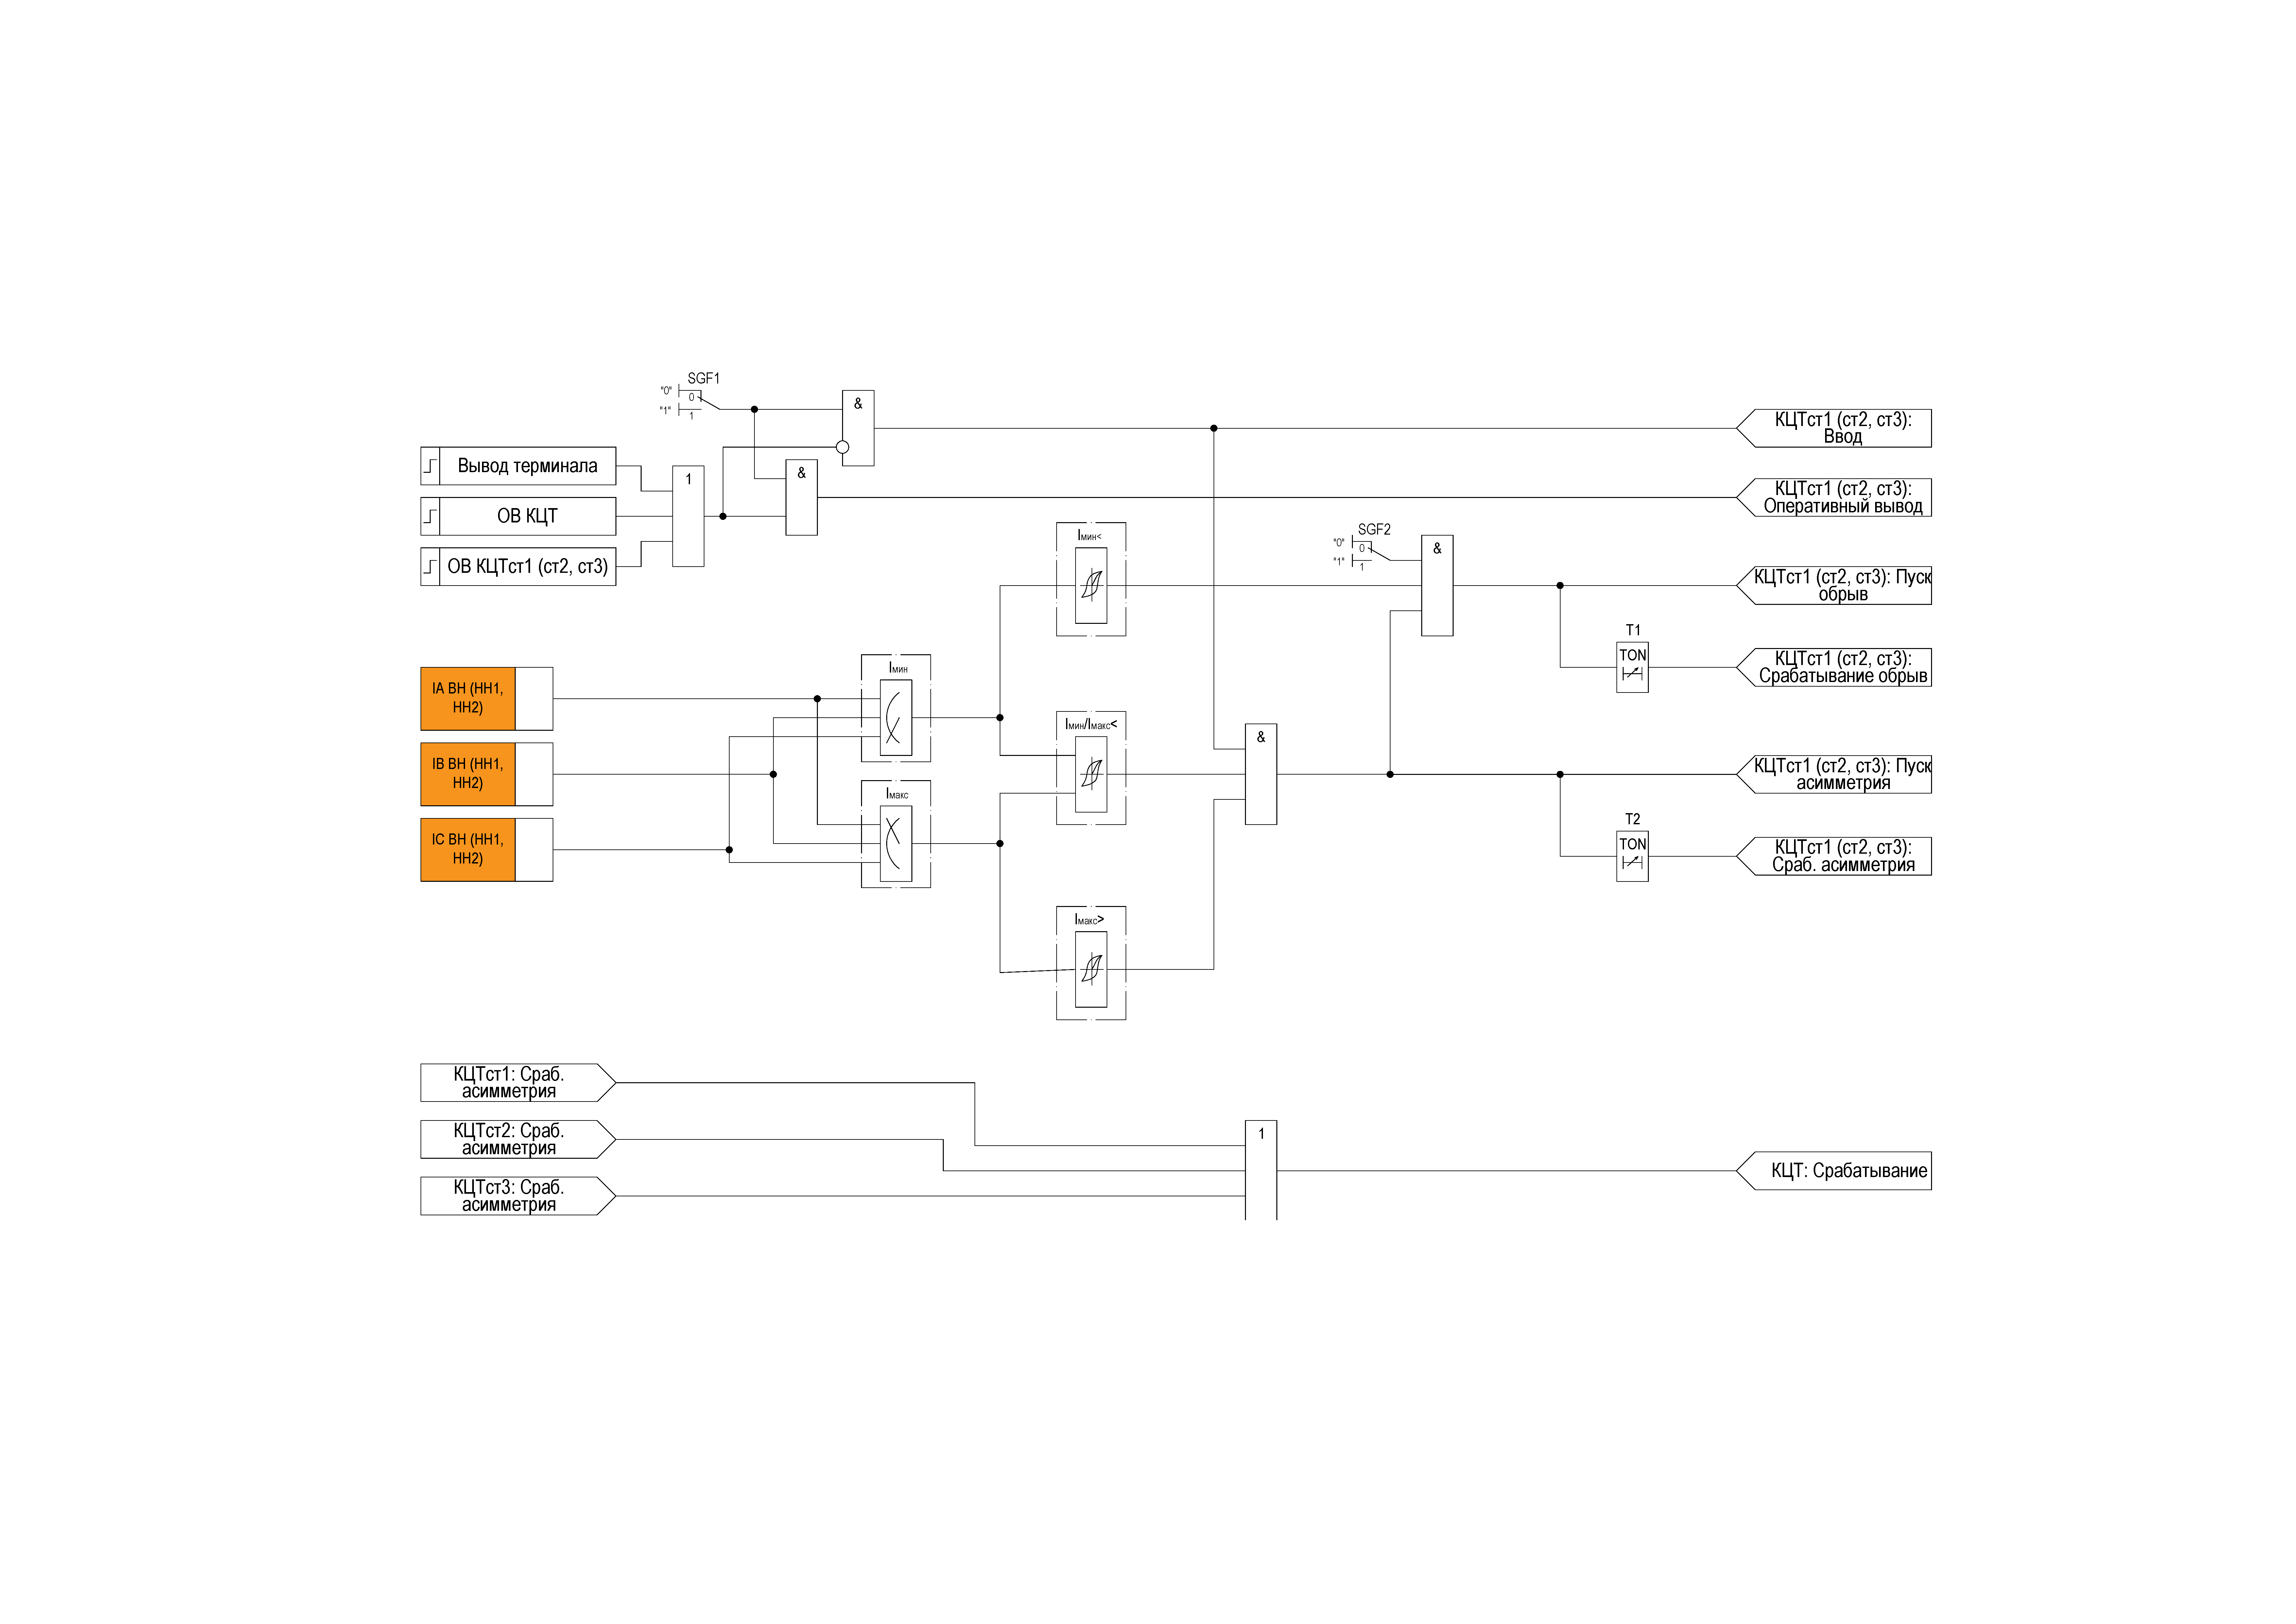
\includegraphics[width=1\textwidth,height=1\textheight,keepaspectratio]{img12.pdf}
\captionof{figure}{Функциональная схема <<КЦТ>>}
\label{kzt:img1}
\end{figure}

\small
\begin{longtable}{|>{\centering\arraybackslash}m{5.3cm}|>{\centering\arraybackslash}m{3.3cm}|>{\centering\arraybackslash}m{4.2cm}|>{\centering\arraybackslash}m{1.8cm}|>{\centering\arraybackslash}m{1cm}|}
\caption{Параметры для настройки функции контроля токовых цепей <<КЦТ>>\hfill\vspace{-0.5\baselineskip}}\label{kzt:tbl1}\\ 
\hline
\rowcolor{gray!30}
Параметр (Параметр на ИЧМ) & Условное обозначение на схеме & Значение/ Диапазон & Единица измерения & Шаг \\ 
\hline
\endfirsthead
\caption*{\hspace{3pt}\emph{Продолжение таблицы \ref{kzt:tbl1}\hfill\vspace{-0.5\baselineskip}}} \\ % сделано по ГОСТ 2.105 п.6.8.7
\hline
\rowcolor{gray!30}
Параметр (Параметр на ИЧМ) & Условное обозначение на схеме & Значение/ Диапазон & Единица измерения & Шаг \\ 
\endhead
\endfoot
\endlastfoot
\centering Ввод функции в работу (Ввод\_функции) & \centering SGF1 & \centering 0 = Не предусмотрено\\1 = Предусмотрено & \centering -- & \centering \arraybackslash -- \\
\hline
\centering Режим контроля обрыва провода (Контр\_обр\_пров) & \centering SGF2 & \centering 0 = Не предусмотрено\\1 = Предусмотрено & \centering -- & \centering \arraybackslash -- \\
\hline
\centering Номинальный ток токового входа терминала (Iном) & \centering -- & \centering 0,2 ... 5,0 & \centering А & \centering \arraybackslash 0,1 \\
\hline
\centering Минимальное значение фазного тока (Iмин) & \centering Iмин$<$ & \centering 0,05 ... 1,00 & \centering о.е. & \centering \arraybackslash 0,01 \\
\hline
\centering Коэффициент симметрии (Kсим) & \centering Iмин/Iмакс$<$ & \centering 0,10 ... 0,95 & \centering о.е. & \centering \arraybackslash 0,01 \\
\hline
\centering Минимальная величина максимального из фазных токов (LIсим) & \centering Iмакс$>$ & \centering 0,01 ... 2,00 & \centering о.е. & \centering \arraybackslash 0,01 \\
\hline
\centering Выдержка времени на срабатывание по критерию обрыва фазы (Tобрыв) & \centering T1 & \centering 0,00 ... 100,00 & \centering с & \centering \arraybackslash 0,01 \\
\hline
\centering Выдержка времени на срабатывание по асимметрии токов (Tасим) & \centering T2 & \centering 0,00 ... 100,00 & \centering с & \centering \arraybackslash 0,01 \\
\hline
\end{longtable}
\normalsize



\item
Функция контроля исправности токовых цепей стороны трансформатора (<<КЦТст>>) предназначена для контроля вторичных цепей трансформаторов тока одной из сторон силового трансформатора (возможен контроль токовых цепей до трех сторон). Разомкнутые или короткозамкнутые цепи трансформаторов тока могут вызвать как ложное срабатывание, так и несрабатывание защит.
\item
Функция <<КЦТст>> обнаруживает обрывы цепей, короткие замыкания в цепях переменного тока по наличию несимметрии. Наличие несимметрии предполагается, если выполняются следующие условия:

\begin{equation*}
\frac{\left | I_{\textsl{мин.изм.}} \right |}{\left | I_{\textsl{макс.изм.}} \right |}< K_{\textsl{сим}},
\end{equation*}
\begin{equation*}
I_{\textsl{макс.изм.}}> LI_{\textsl{сим}},
\end{equation*}
\begin{eqexpl}[25mm]
\item{$I_{\textsl{мин.изм.}}$, $I_{\textsl{макс.изм.}}$ }минимальный и максимальный измеренные фазные токи соответственно;
\item{$K_{\textsl{сим}}$}коэффициент симметрии;
\item{$LI_{\textsl{сим}}$}минимальная величина максимального из фазных токов.
\end{eqexpl}
В случае выполнения данных условий в течение выдержки времени <<Tасим>> происходит срабатывание функции.
\item
Характеристика срабатывания КЦТ стороны приведена на рисунке \ref{kitz:char}.
\vspace{1mm}
\begin{figure}[H]
\centering
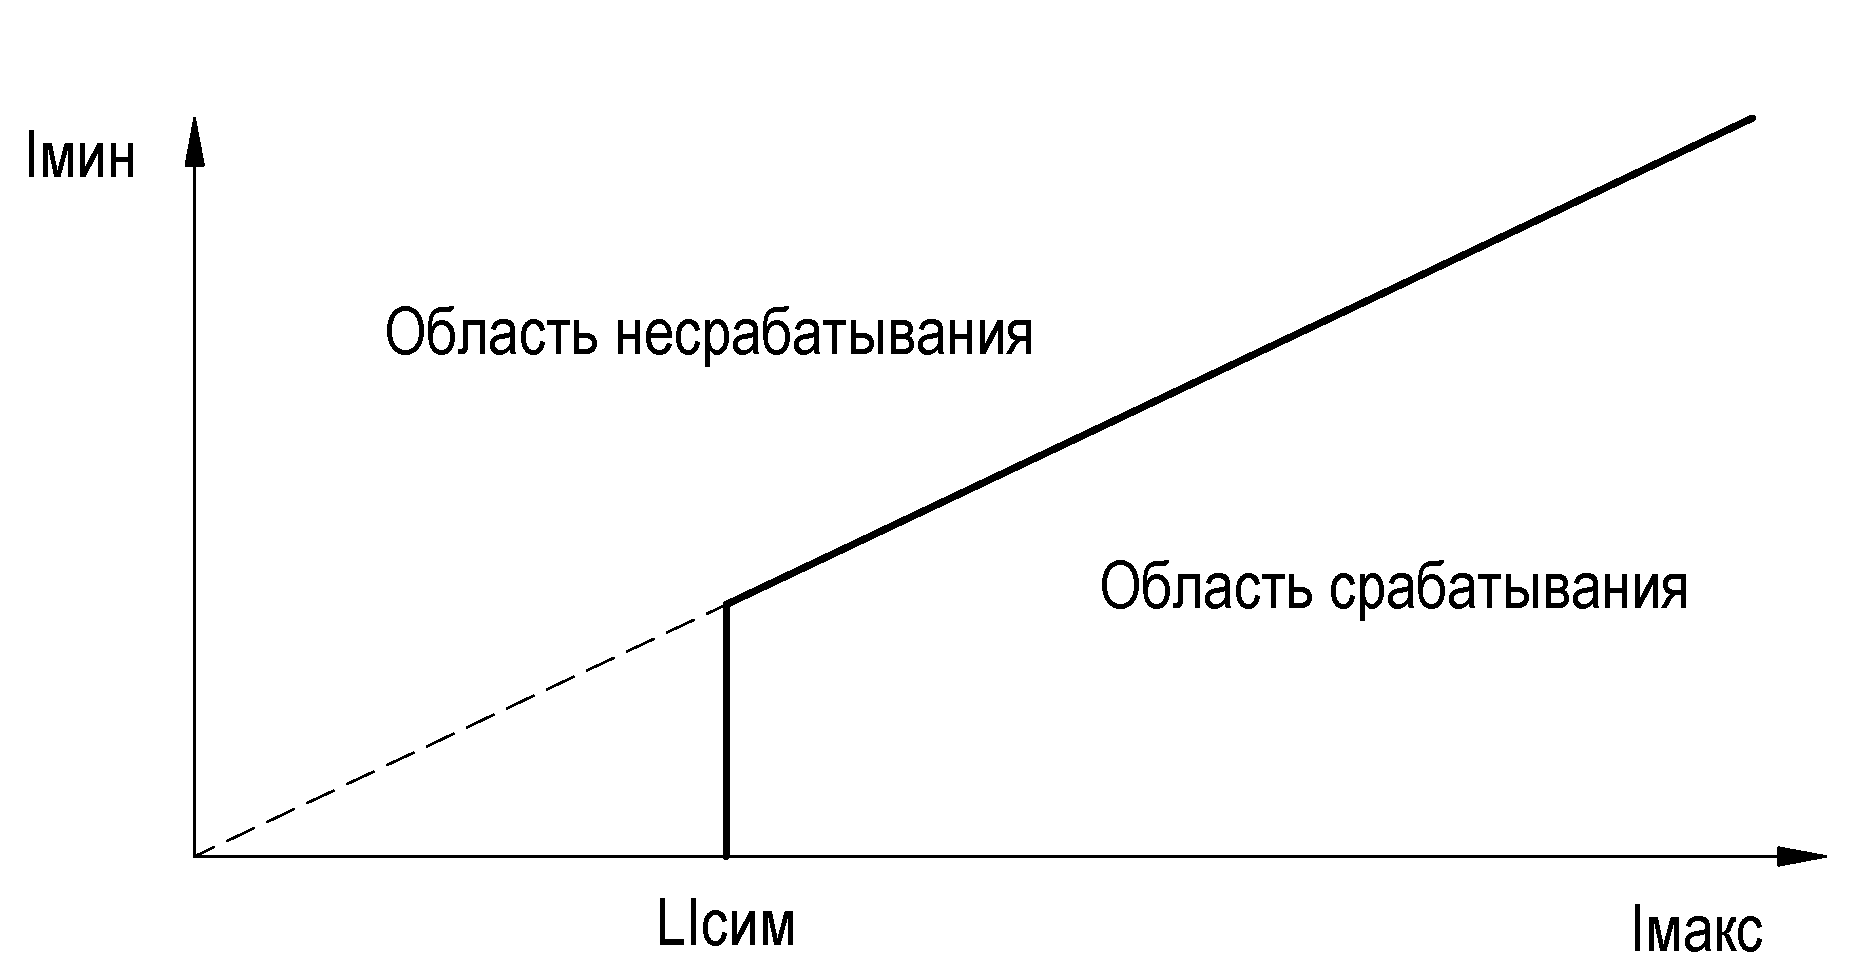
\includegraphics[width=0.55\textwidth,height=0.55\textheight,keepaspectratio]{img13.pdf}
\captionof{figure}{Характеристика срабатывания функции контроля токовых цепей стороны трансформатора}\label{kitz:char}
\end{figure}

\end{enumerate}
\FloatBarrier % Все float'ы ДО этой строки будут размещены здесь.
\needspace{4\baselineskip}
\color{uniblue}{\subsection{Защита от потери охлаждения (ЗПО)}\label{sec:zpo}}
\color{black}

\begin{enumerate}[label=\arabic{section}.\arabic{subsection}.\arabic*, labelsep=4pt, leftmargin=0pt, itemindent=57pt]

\item
Функция <<ЗПО>> служит для формирования сигнала на отключение трансформатора при отказе системы охлаждения трансформатора, дополнительными контролируемыми факторами для формирования сигнала отключения могут являться сигналы срабатывания токовых органов ЗПО (см. подраздел \ref{sec:tozpo}) и датчика температуры масла.
\item
Трансформатор с высшим напряжением 35 кВ может оснащаться системой охлаждения типа <<Д>> (естественная циркуляция масла с принудительной циркуляцией воздуха). Для таких трансформаторов необходимо предусматривать автоматическое управление пуском и остановом вентиляторов обдува. В случае неисправности системы охлаждения и превышения нормальных параметров эксплуатации трансформатора (повышение температуры верхних слоев масла, превышение номинального тока трансформатора) в некоторых случаях может потребоваться отключение трансформатора. 
\item
Ввод функции в работу на этапе параметрирования устройства осуществляется программным переключателем SGF1 <<Ввод\_функции>>. Информация о введенной функции отображается выходным сигналом <<ЗПО: Ввод>>. 
\item
Функция <<ЗПО>> может быть выведена из работы оперативно путем активации сигнала <<ОВ ЗПО>>, что характеризуется активным состоянием сигнала <<ЗПО: Оперативный вывод>> на выходе функции. 
\item
При активном состоянии входного сигнала <<ЗПО~на~сигн>> действие отключающей логики переводится на сигнал.
\item
Пуск ЗПО происходит при приеме сигнала <<Отказ сист. охл.>> от системы охлаждения, формирование сигнала отключения происходит через выдержку времени таймера T1 (уставка <<Тср>>). При этом возможен контроль выполнения следующих условий:
\begin{itemize}
\item срабатывание токовых органов по сторонам ВН, НН (возможная уставка срабатывания -- $\textsl{1,05}I_\textsl{ном}$), управляется программным переключателем SGF2 <<Контр\_тока>>;
\item срабатывание датчика температуры (возможная уставка срабатывания -- $\textsl{55}^\circ C$), управляется программным переключателем SGF3 <<Контр\_темп\_масла>>.
\end{itemize}
\par {\small{ \textls[100]{Примечание} -- Возможные уставки срабатывания приведены в качестве примера из ГОСТ Р 52719-2007, при настройке функции необходимо руководствоваться в том числе и требованиями завода-изготовителя трансформатора.}}

\item
Алгоритм работы <<ЗПО>> выполнен в соответствии с рисунком \ref{zpo:img1}. В таблице \ref{zpo:tbl1} приведены параметры, необходимые для настройки функции <<ЗПО>>.

\vspace{3mm}
\begin{figure}[!h]
\centering
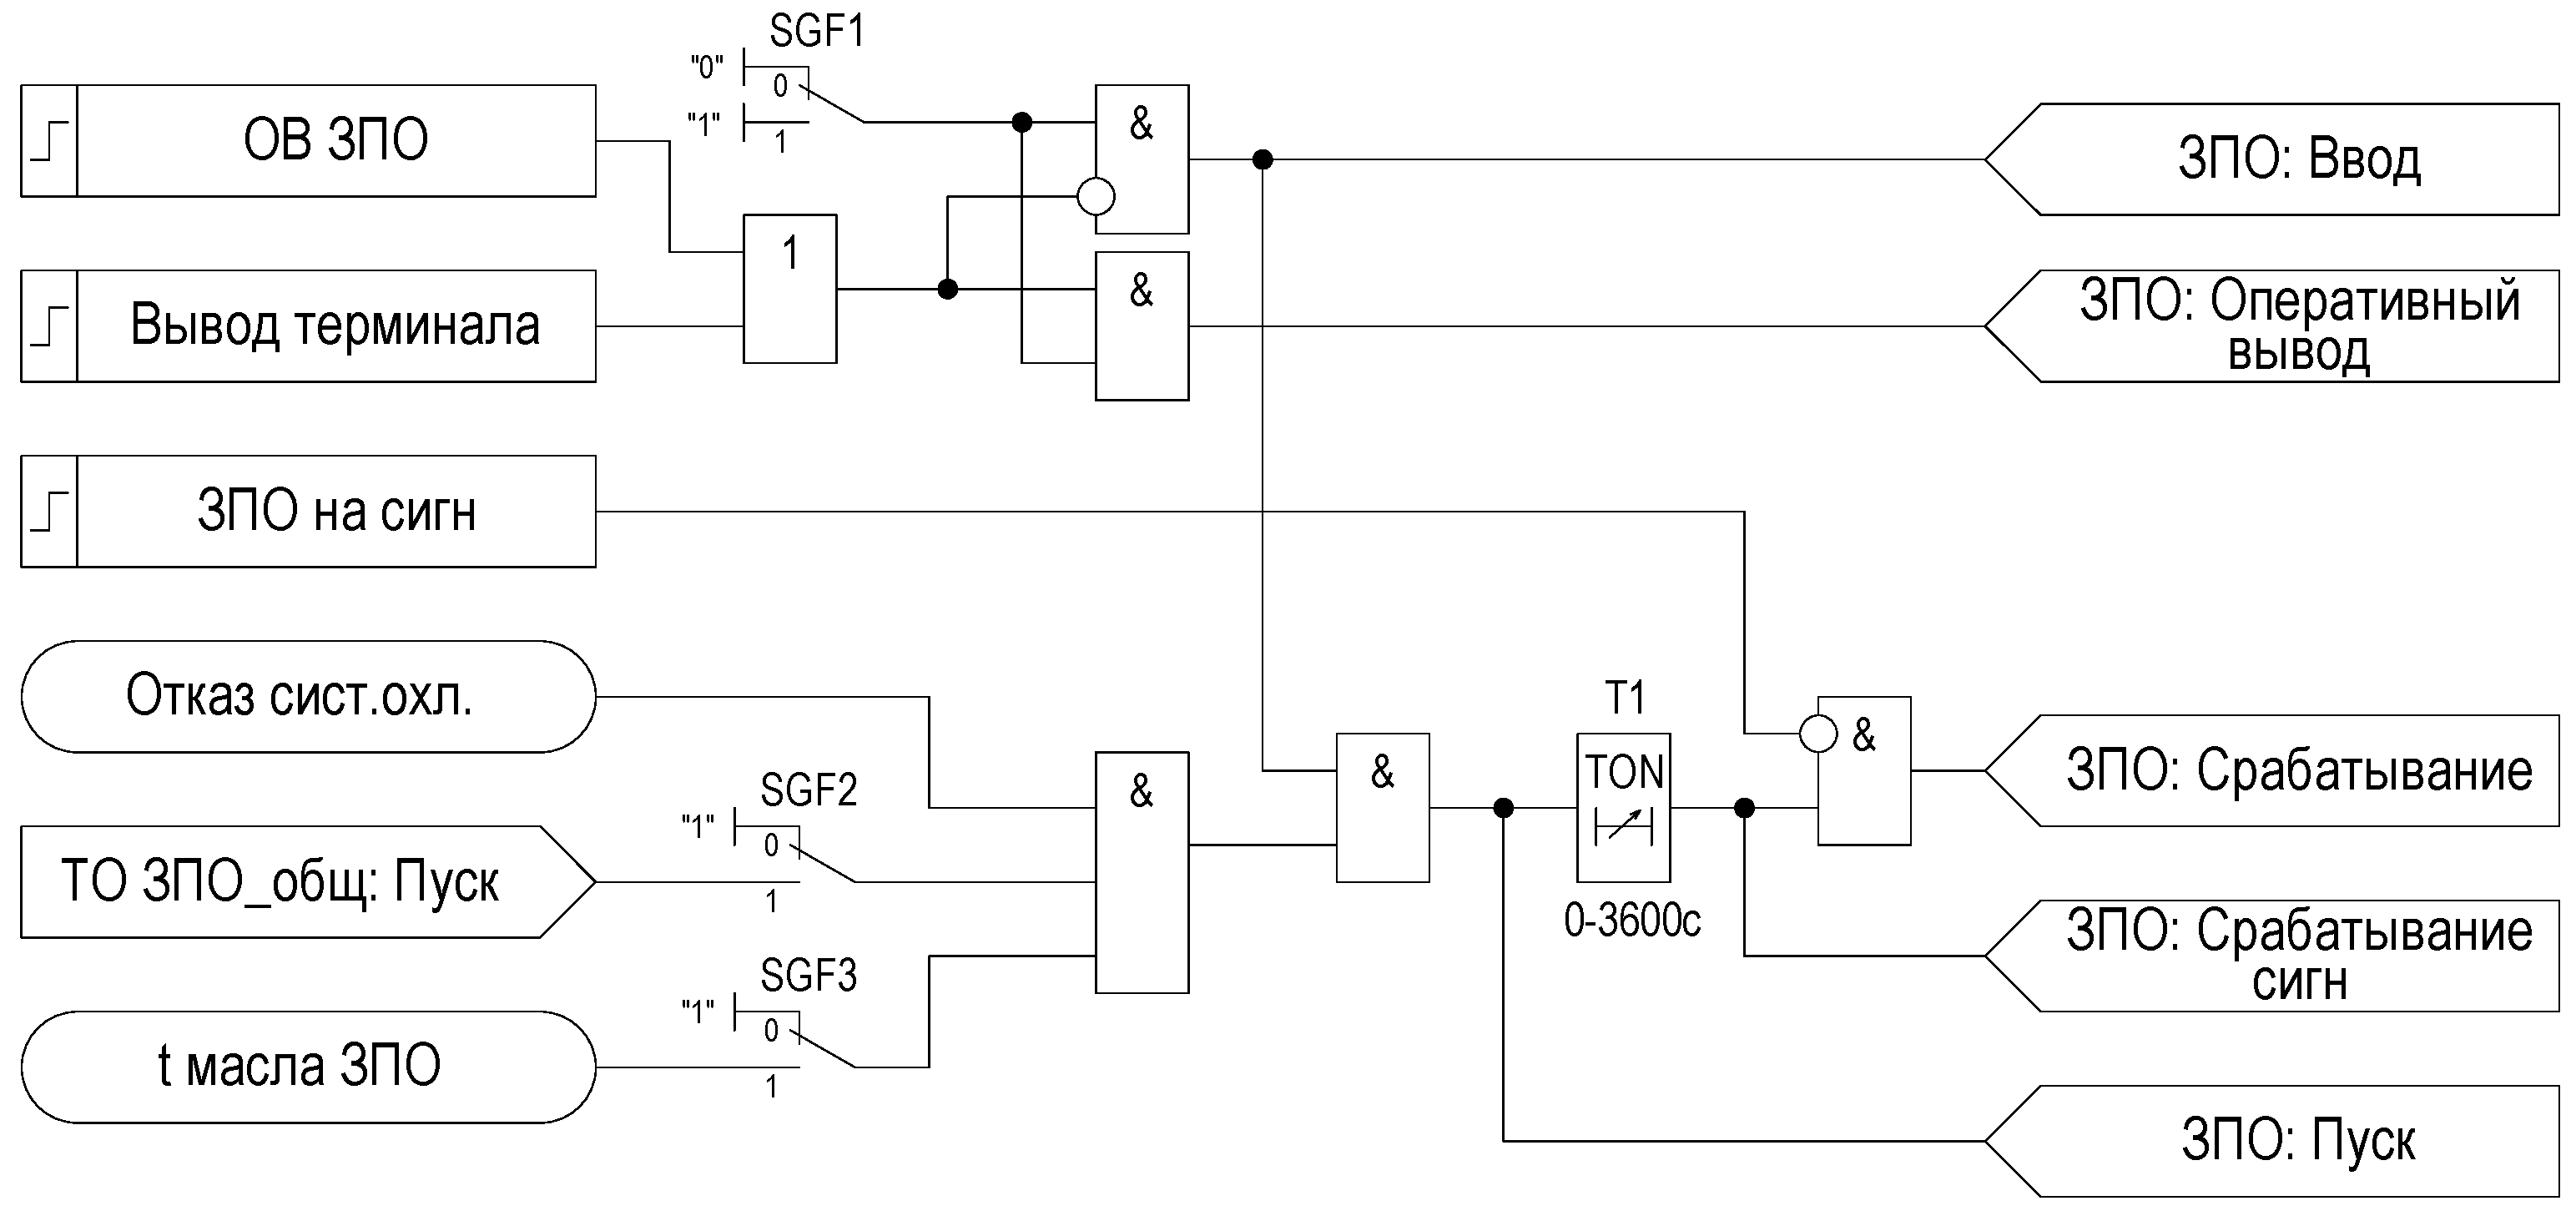
\includegraphics[width=1\textwidth,height=1\textheight,keepaspectratio]{img14.pdf}
\captionof{figure}{Функциональная схема <<ЗПО>>}\label{zpo:img1}
\end{figure}
\small
\begin{longtable}{|>{\centering\arraybackslash}m{5.3cm}|>{\centering\arraybackslash}m{3.3cm}|>{\centering\arraybackslash}m{4.2cm}|>{\centering\arraybackslash}m{1.8cm}|>{\centering\arraybackslash}m{1cm}|}
\caption{Параметры для настройки функции <<ЗПО>>\hfill\vspace{-0.5\baselineskip}}\label{zpo:tbl1}\\ 
\hline
\rowcolor{gray!30}
Параметр (Параметр на ИЧМ) & Условное обозначение на схеме & Значение/ Диапазон & Единица измерения & Шаг \\ 
\hline
\endfirsthead
\caption*{\hspace{3pt}\emph{Продолжение таблицы \ref{zpo:tbl1}\hfill\vspace{-0.5\baselineskip}}} \\ % сделано по ГОСТ 2.105 п.6.8.7
\hline
\rowcolor{gray!30}
Параметр (Параметр на ИЧМ) & Условное обозначение на схеме & Значение/ Диапазон & Единица измерения & Шаг \\ 
\endhead
\endfoot
\endlastfoot
\centering Ввод функции в работу (Ввод\_функции) & \centering SGF1 & \centering 0 = Не предусмотрено\\1 = Предусмотрено & \centering -- & \centering \arraybackslash -- \\
\hline
\centering Контроль тока (Контр\_тока) & \centering SGF2 & \centering 0 = Не предусмотрено\\1 = Предусмотрено & \centering -- & \centering \arraybackslash -- \\
\hline
\centering Контроль температуры масла (Контр\_темп\_масла) & \centering SGF3 & \centering 0 = Не предусмотрено\\1 = Предусмотрено & \centering -- & \centering \arraybackslash -- \\
\hline
\centering Выдержка времени срабатывания (Tср) & \centering T1 & \centering 0 ... 3600 & \centering с & \centering \arraybackslash 1 \\
\hline
\end{longtable}
\normalsize

\end{enumerate}
\FloatBarrier % Все float'ы ДО этой строки будут размещены здесь.

\needspace{3\baselineskip}
\color{uniblue}{\subsection{Токовые органы защиты от потери охлаждения (ТО ЗПО)}\label{sec:tozpo}}
\color{black}

\begin{enumerate}[label=\arabic{section}.\arabic{subsection}.\arabic*, labelsep=4pt, leftmargin=0pt, itemindent=57pt]

\item
Функциональный блок <<ТО ЗПО>> является вспомогательным токовым органом для работы защиты от потери охлаждения (см. подраздел \ref{sec:zpo}) и имеет в своем составе токовые органы по каждой из трех сторон трансформатора 35 кВ (ТО ВН, ТО НН1, ТО НН2).
\item
Ввод пускового токового органа каждой стороны в работу на этапе параметрирования устройства осуществляется своим программным переключателем SGF1 <<Ввод\_функции>>.
\item
Функциональный блок <<ТО ЗПО>> может быть выведен из работы оперативно путем активации сигнала <<ОВ ТО ЗПО>>, дополнительно к этому существует возможность оперативного вывода функции контроля тока каждой стороны отдельно путем активации сигналов <<ОВ ТО ЗПО ВН>>, <<ОВ ТО ЗПО НН1>>, <<ОВ ТО ЗПО НН2>>, что характеризуется активным состоянием сигналов <<ТО ЗПО ВН: Оперативный вывод>>, <<ТО ЗПО НН1: Оперативный вывод>>, <<ТО ЗПО НН2: Оперативный вывод>> соответственно для сторон ВН, НН1 и НН2 на выходе функции.
\item
При превышении заданной уставки по току любой из сторон трансформатора выдается обобщенный сигнал пуска <<ТО ЗПО: Пуск>> для защиты от потери охлаждения трансформатора.
\item
В качестве измерительных органов в токовых органах применяются ИО тока максимального действия, принцип работы которых заключается в пофазном сравнении действующего значения основной гармоники тока с уставкой срабатывания. Коэффициент возврата порогового элемента равен 0,95.
\item
Алгоритм работы <<ТО ЗПО>> выполнен в соответствии с рисунком \ref{tozpo:img1}. В таблице \ref{tozpo:tbl1} приведены параметры, необходимые для настройки функционального блока <<ТО ЗПО>>.

\vspace{3mm}
\begin{figure}[!h]
\centering
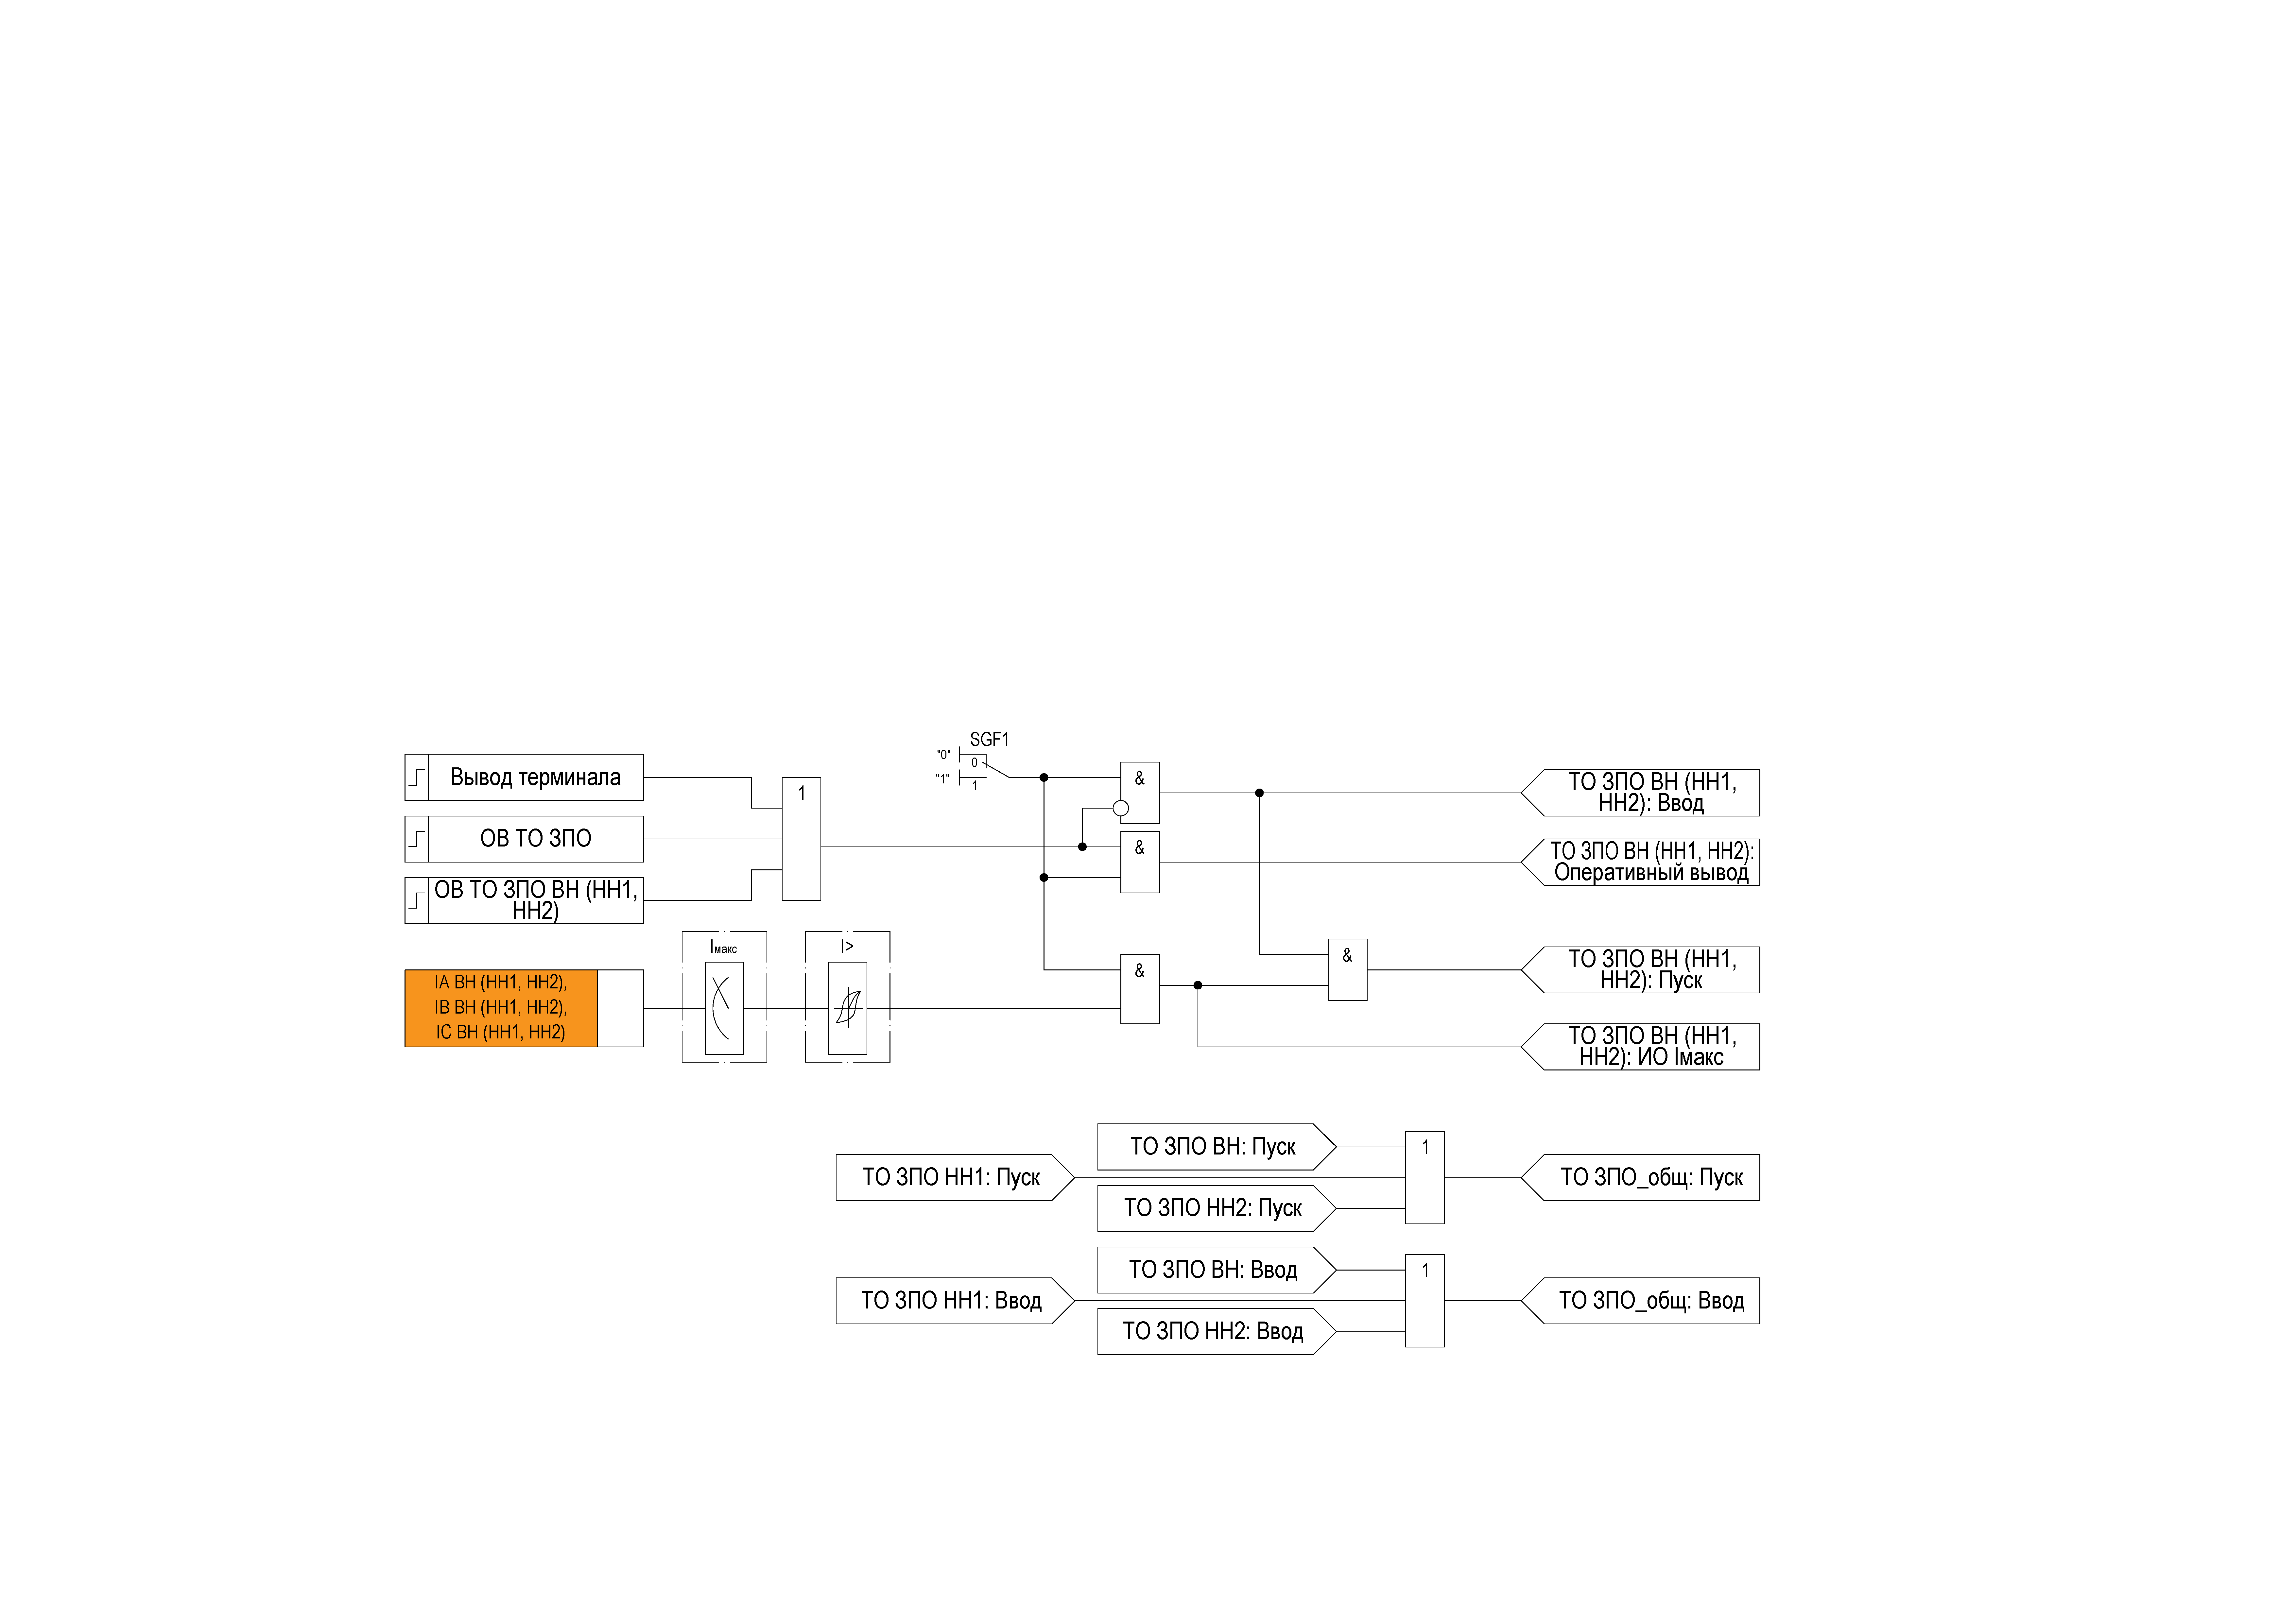
\includegraphics[width=1\textwidth,height=1\textheight,keepaspectratio]{img15.pdf}
\captionof{figure}{Функциональная схема <<ТО ЗПО>>}\label{tozpo:img1}
\end{figure}

\small
\begin{longtable}{|>{\centering\arraybackslash}m{5.3cm}|>{\centering\arraybackslash}m{3.3cm}|>{\centering\arraybackslash}m{4.2cm}|>{\centering\arraybackslash}m{1.8cm}|>{\centering\arraybackslash}m{1cm}|}
\caption{Параметры для настройки функций в составе функционального блока <<ТО ЗПО>>\hfill\vspace{-0.5\baselineskip}}\label{tozpo:tbl1}\\ 
\hline
\rowcolor{gray!30}
Параметр (Параметр на ИЧМ) & Условное обозначение на схеме & Значение/ Диапазон & Единица измерения & Шаг \\ 
\hline
\endfirsthead
\caption*{\hspace{3pt}\emph{Продолжение таблицы \ref{tozpo:tbl1}\hfill\vspace{-0.5\baselineskip}}} \\ % сделано по ГОСТ 2.105 п.6.8.7
\hline
\rowcolor{gray!30}
Параметр (Параметр на ИЧМ) & Условное обозначение на схеме & Значение/ Диапазон & Единица измерения & Шаг \\ 
\endhead
\endfoot
\endlastfoot
\centering Ввод функции в работу (Ввод\_функции) & \centering SGF1 & \centering 0 = Не предусмотрено\\1 = Предусмотрено & \centering -- & \centering \arraybackslash -- \\
\hline
\centering Ток срабатывания (Iср) & \centering I$>$ & \centering 0,10 ... 30,00 & \centering о.е. & \centering \arraybackslash 0,01 \\
\hline
\end{longtable}
\normalsize

\end{enumerate}
\FloatBarrier % Все float'ы ДО этой строки будут размещены здесь.

\needspace{4\baselineskip}
\color{uniblue}{\subsection{Защита от перегрузки трансформатора (ЗП)}}
\color{black}

\begin{enumerate}[label=\arabic{section}.\arabic{subsection}.\arabic*, labelsep=4pt, leftmargin=0pt, itemindent=57pt]

\item
Функциональный блок <<ЗП>> служит для контроля перегрузки трансформатора по току и имеет в своем составе функции контроля перегрузки по каждой из трех сторон трансформатора 35 кВ (ЗП ВН, ЗП НН1, ЗП НН2). 
\item
Ввод защиты от перегрузки каждой стороны в работу на этапе параметрирования устройства осуществляется своим программным переключателем SGF1 <<Ввод\_функции>>. Информация о введенной функции защиты от перегрузки каждой стороны отображается выходным сигналом для каждой функции (<<ЗП ВН: Ввод>>, <<ЗП НН1: Ввод>>, <<ЗП НН2: Ввод>>).
\item
Функциональный блок <<ЗП>> может быть выведен из работы оперативно путем активации сигнала <<ОВ ЗП>>, дополнительно к этому существует возможность оперативного вывода защиты от перегрузки каждой стороны отдельно путем активации сигналов <<ОВ ЗП ВН>>, <<ОВ ЗП НН1>>, <<ОВ ЗП НН2>>, что характеризуется активным состоянием сигналов <<ЗП ВН: Оперативный вывод>>, <<ЗП НН1: Оперативный вывод>>, <<ЗП НН2: Оперативный вывод>> соответственно для сторон ВН, НН1 и НН2 на выходе функции.
\item\label{zp:punkt1}
Функции в составе <<ЗП>> контролируют повышение любого фазного тока (\textsl{IA, IB, IC}) каждой из сторон трансформатора выше заданной уставки, при превышении заданной уставки по току через выдержку времени таймера T1 (уставка <<Тср>>) выдается сигнализация о перегрузке трансформатора (выходной сигнал <<ЗП: Срабатывание>>). 
\item
При активном состоянии входного сигнала <<ЗП на откл>> действие защиты от перегрузки вводится на отключение. В этом случае одновременно с активацией выходного сигнала <<ЗП: Срабатывание>> выдается сигнал на отключение трансформатора <<ЗП: Сраб. на откл>>.
\item
В качестве измерительных органов в защите от перегрузки применяется ИО тока максимального действия, принцип работы которых заключается в пофазном сравнении действующего значения основной гармоники тока с уставкой срабатывания. Коэффициент возврата порогового элемента равен 0,95.
\item
Алгоритм работы <<ЗП>> выполнен в соответствии с рисунком \ref{zp:img1}. В таблице \ref{zp:tbl1} приведены параметры, необходимые для настройки функционального блока <<ЗП>>.

\vspace{3mm}
\begin{figure}[!h]
\centering
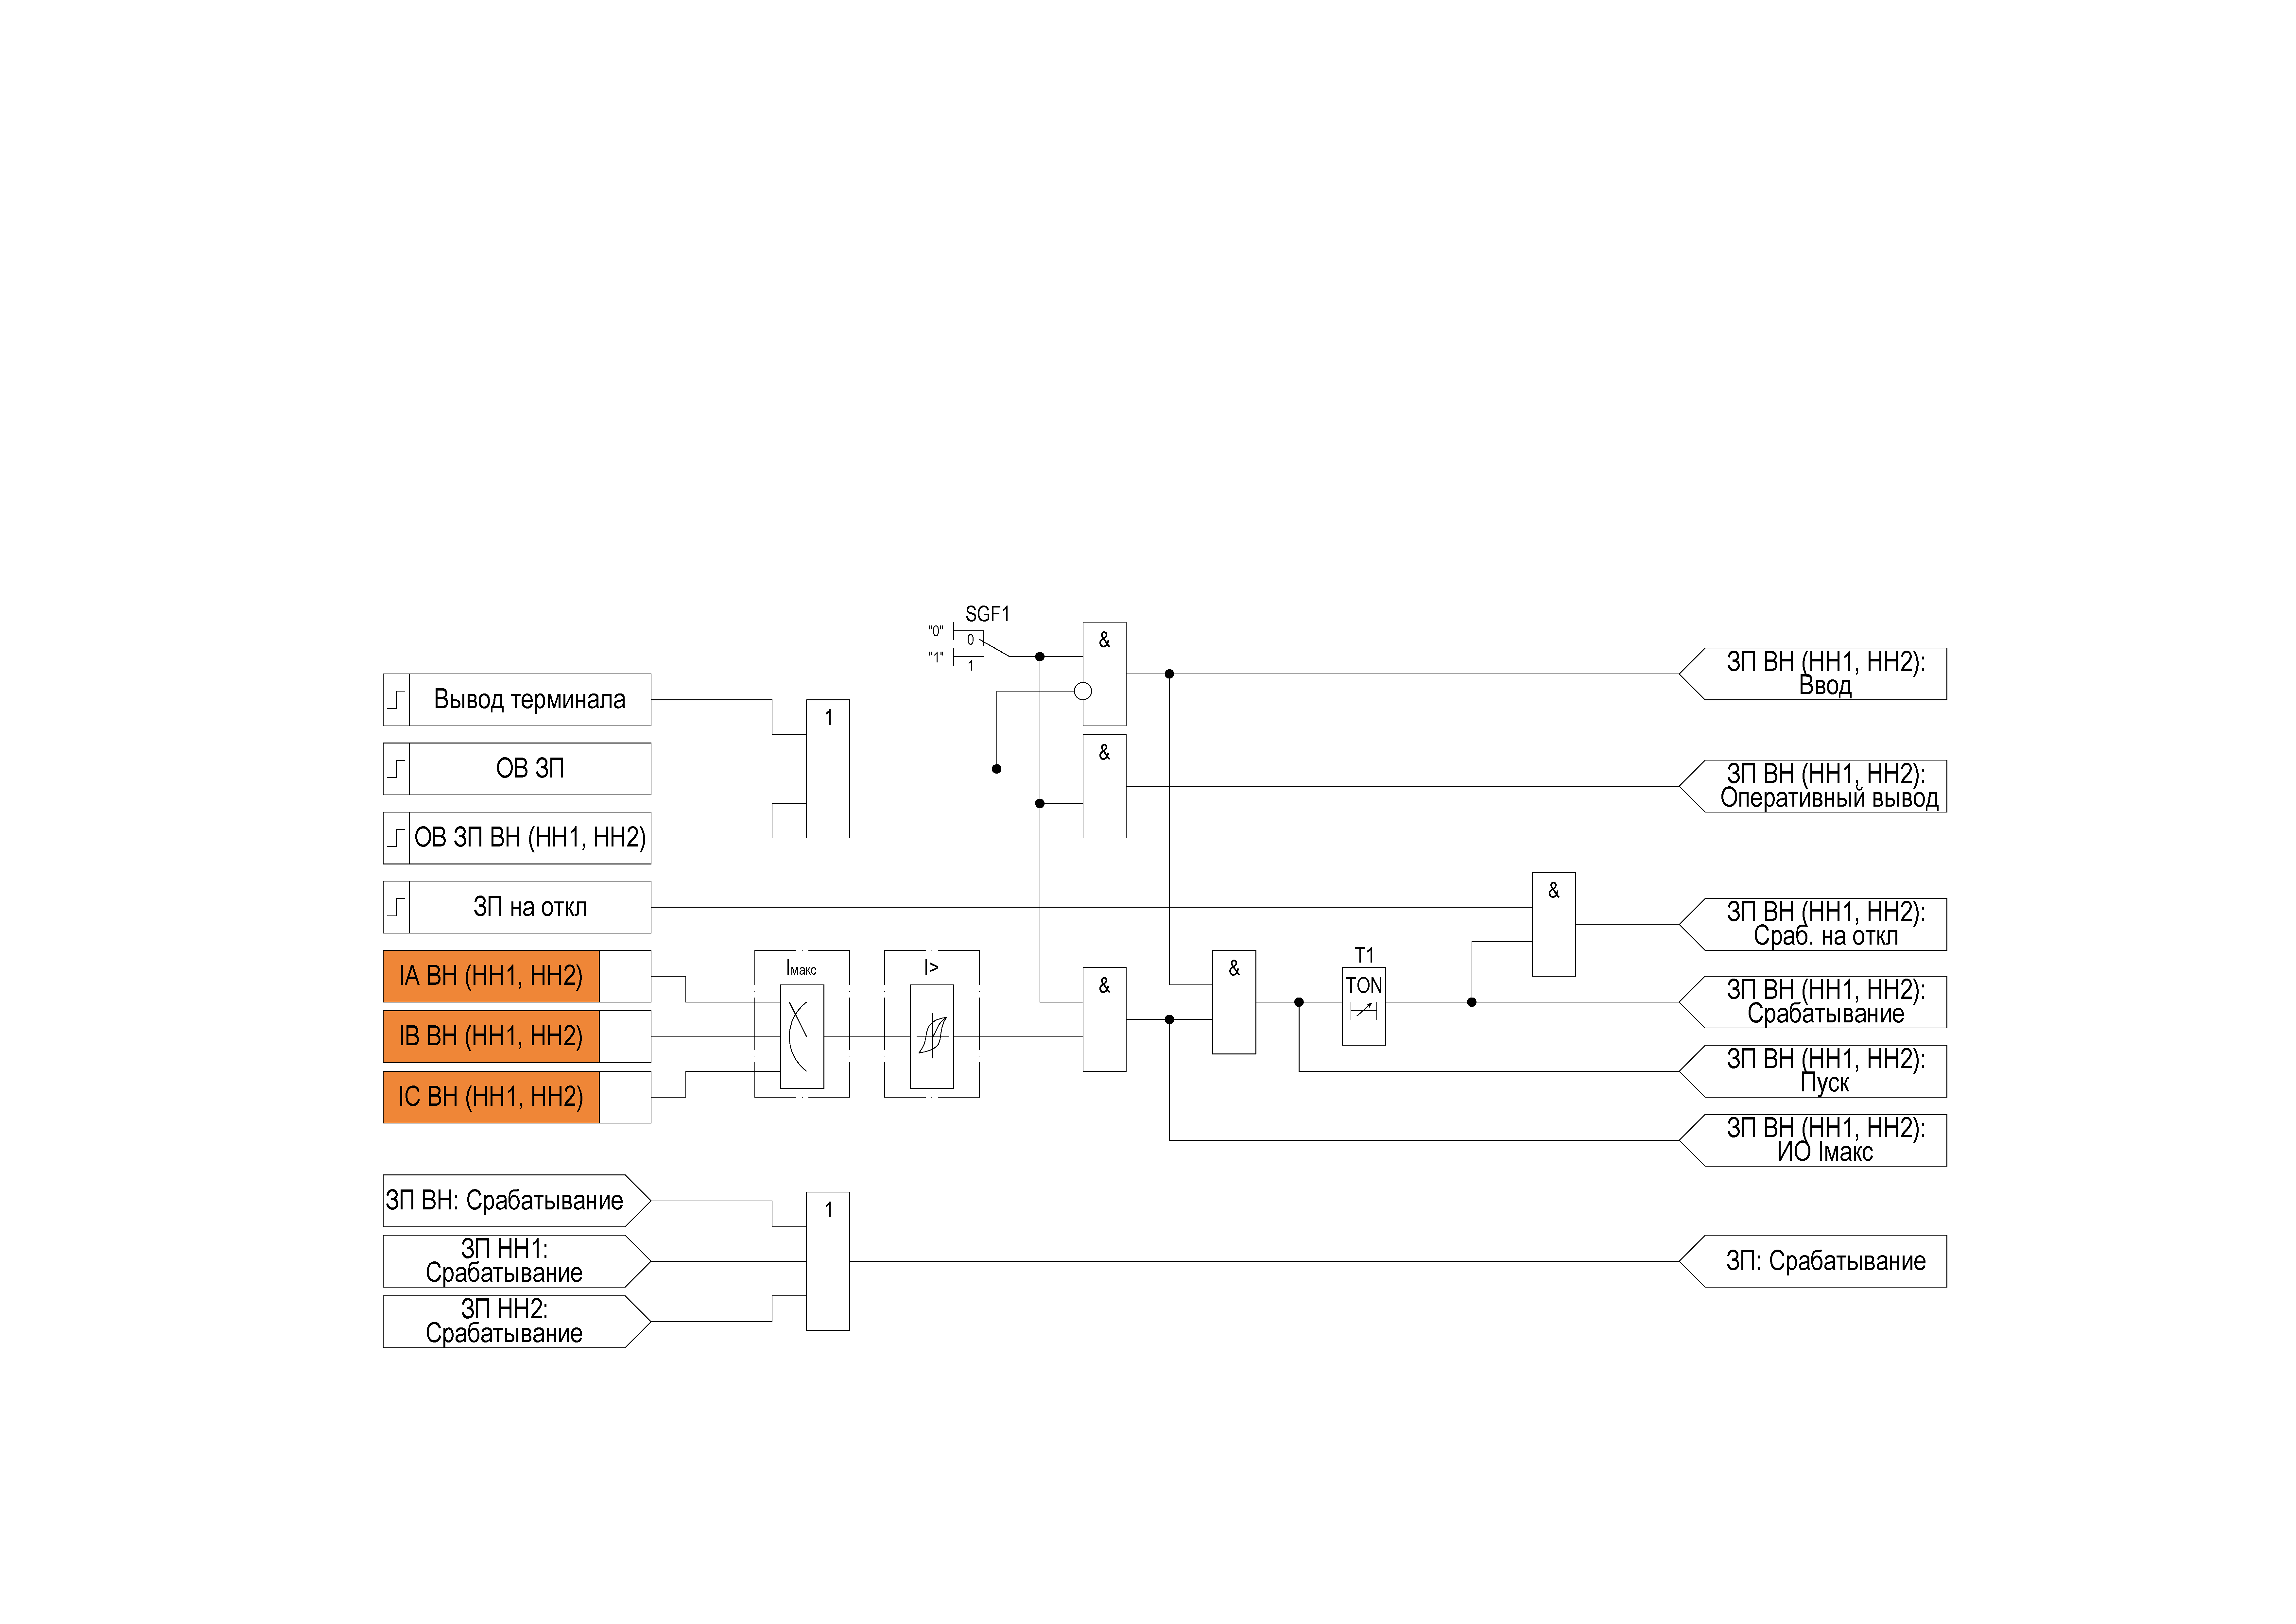
\includegraphics[width=1\textwidth,height=1\textheight,keepaspectratio]{img16.pdf}
\captionof{figure}{Функциональная схема <<ЗП>>}\label{zp:img1}
\end{figure}

\small
\begin{longtable}{|>{\centering\arraybackslash}m{5.3cm}|>{\centering\arraybackslash}m{3.3cm}|>{\centering\arraybackslash}m{4.2cm}|>{\centering\arraybackslash}m{1.8cm}|>{\centering\arraybackslash}m{1cm}|}
\caption{Параметры для настройки функций <<ЗП ВН>>, <<ЗП НН1>>, <<ЗП НН2>> в составе функционального блока <<ЗП>>\hfill\vspace{-0.5\baselineskip}}\label{zp:tbl1}\\ 
\hline
\rowcolor{gray!30}
Параметр (Параметр на ИЧМ) & Условное обозначение на схеме & Значение/ Диапазон & Единица измерения & Шаг \\ 
\hline
\endfirsthead
\caption*{\hspace{3pt}\emph{Продолжение таблицы \ref{zp:tbl1}\hfill\vspace{-0.5\baselineskip}}} \\ % сделано по ГОСТ 2.105 п.6.8.7
\hline
\rowcolor{gray!30}
Параметр (Параметр на ИЧМ) & Условное обозначение на схеме & Значение/ Диапазон & Единица измерения & Шаг \\ 
\endhead
\endfoot
\endlastfoot
\centering Ввод функции в работу (Ввод\_функции) & \centering SGF1 & \centering 0 = Не предусмотрено\\1 = Предусмотрено & \centering -- & \centering \arraybackslash -- \\
\hline
\centering Ток срабатывания (Iср) & \centering I$>$ & \centering 0,10 ... 5,00 & \centering о.е. & \centering \arraybackslash 0,01 \\
\hline
\centering Выдержка времени срабатывания (Tср) & \centering T1 & \centering 0,0 ... 3600,0 & \centering с & \centering \arraybackslash 0,1 \\
\hline
\end{longtable}
\normalsize

\end{enumerate}
\FloatBarrier % Все float'ы ДО этой строки будут размещены здесь.

\needspace{4\baselineskip}
\color{uniblue}{\subsection{Токовые органы пуска охлаждения трансформатора (РТПО)}}
\color{black}

\begin{enumerate}[label=\arabic{section}.\arabic{subsection}.\arabic*, labelsep=4pt, leftmargin=0pt, itemindent=57pt]

\item
Функциональный блок <<РТПО>> служит для формирования сигнала пуска охлаждения трансформатора и имеет в своем составе функции контроля тока по каждой из трех сторон трансформатора 35 кВ (ТО ВН, ТО НН1, ТО НН2). 

\item
Ввод органа пуска охлаждения каждой стороны в работу осуществляется своим программным переключателем SGF1 <<Ввод\_функции>>.
\item
Функциональный блок <<РТПО>> может быть выведен из работы оперативно путем активации сигнала <<ОВ РТПО>>, дополнительно к этому существует возможность оперативного вывода функции контроля тока каждой стороны отдельно путем активации сигналов <<ОВ РТПО ВН>>, <<ОВ РТПО НН1>>, <<ОВ РТПО НН2>>, что характеризуется активным состоянием сигналов <<РТПО ВН: Оперативный вывод>>, <<РТПО НН1: Оперативный вывод>>, <<РТПО НН2: Оперативный вывод>> соответственно для сторон ВН, НН1 и НН2 на выходе функции. 
\item
При превышении заданной уставки по току любой из сторон трансформатора выдается обобщенный сигнал пуска охлаждения трансформатора <<РТПО\_общ: Пуск>>.

\item
Алгоритм работы <<РТПО>> выполнен в соответствии с рисунком \ref{rtpo:img1}. В таблице \ref{rtpo:tbl1} приведены параметры, необходимые для настройки функционального блока <<РТПО>>.

\small
\begin{longtable}{|>{\centering\arraybackslash}m{5.3cm}|>{\centering\arraybackslash}m{3.3cm}|>{\centering\arraybackslash}m{4.2cm}|>{\centering\arraybackslash}m{1.8cm}|>{\centering\arraybackslash}m{1cm}|}
\caption{Параметры для настройки функций <<РТПО ВН>>, <<РТПО НН1>>, <<РТПО НН2>> в составе функционального блока <<РТПО>>\hfill\vspace{-0.5\baselineskip}}\label{rtpo:tbl1}\\ 
\hline
\rowcolor{gray!30}
Параметр (Параметр на ИЧМ) & Условное обозначение на схеме & Значение/ Диапазон & Единица измерения & Шаг \\ 
\hline
\endfirsthead
\caption*{\hspace{3pt}\emph{Продолжение таблицы \ref{rtpo:tbl1}\hfill\vspace{-0.5\baselineskip}}} \\ % сделано по ГОСТ 2.105 п.6.8.7
\hline
\rowcolor{gray!30}
Параметр (Параметр на ИЧМ) & Условное обозначение на схеме & Значение/ Диапазон & Единица измерения & Шаг \\ 
\endhead
\endfoot
\endlastfoot
\centering Ввод функции в работу (Ввод\_функции) & \centering SGF1 & \centering 0 = Не предусмотрено\\1 = Предусмотрено & \centering -- & \centering \arraybackslash -- \\
\hline
\centering Ток срабатывания (Iср) & \centering I$>$ & \centering 0,10 ... 30,00 & \centering о.е. & \centering \arraybackslash 0,01 \\
\hline
\end{longtable}
\normalsize

\vspace{3mm}
\begin{figure}[!h]
\centering
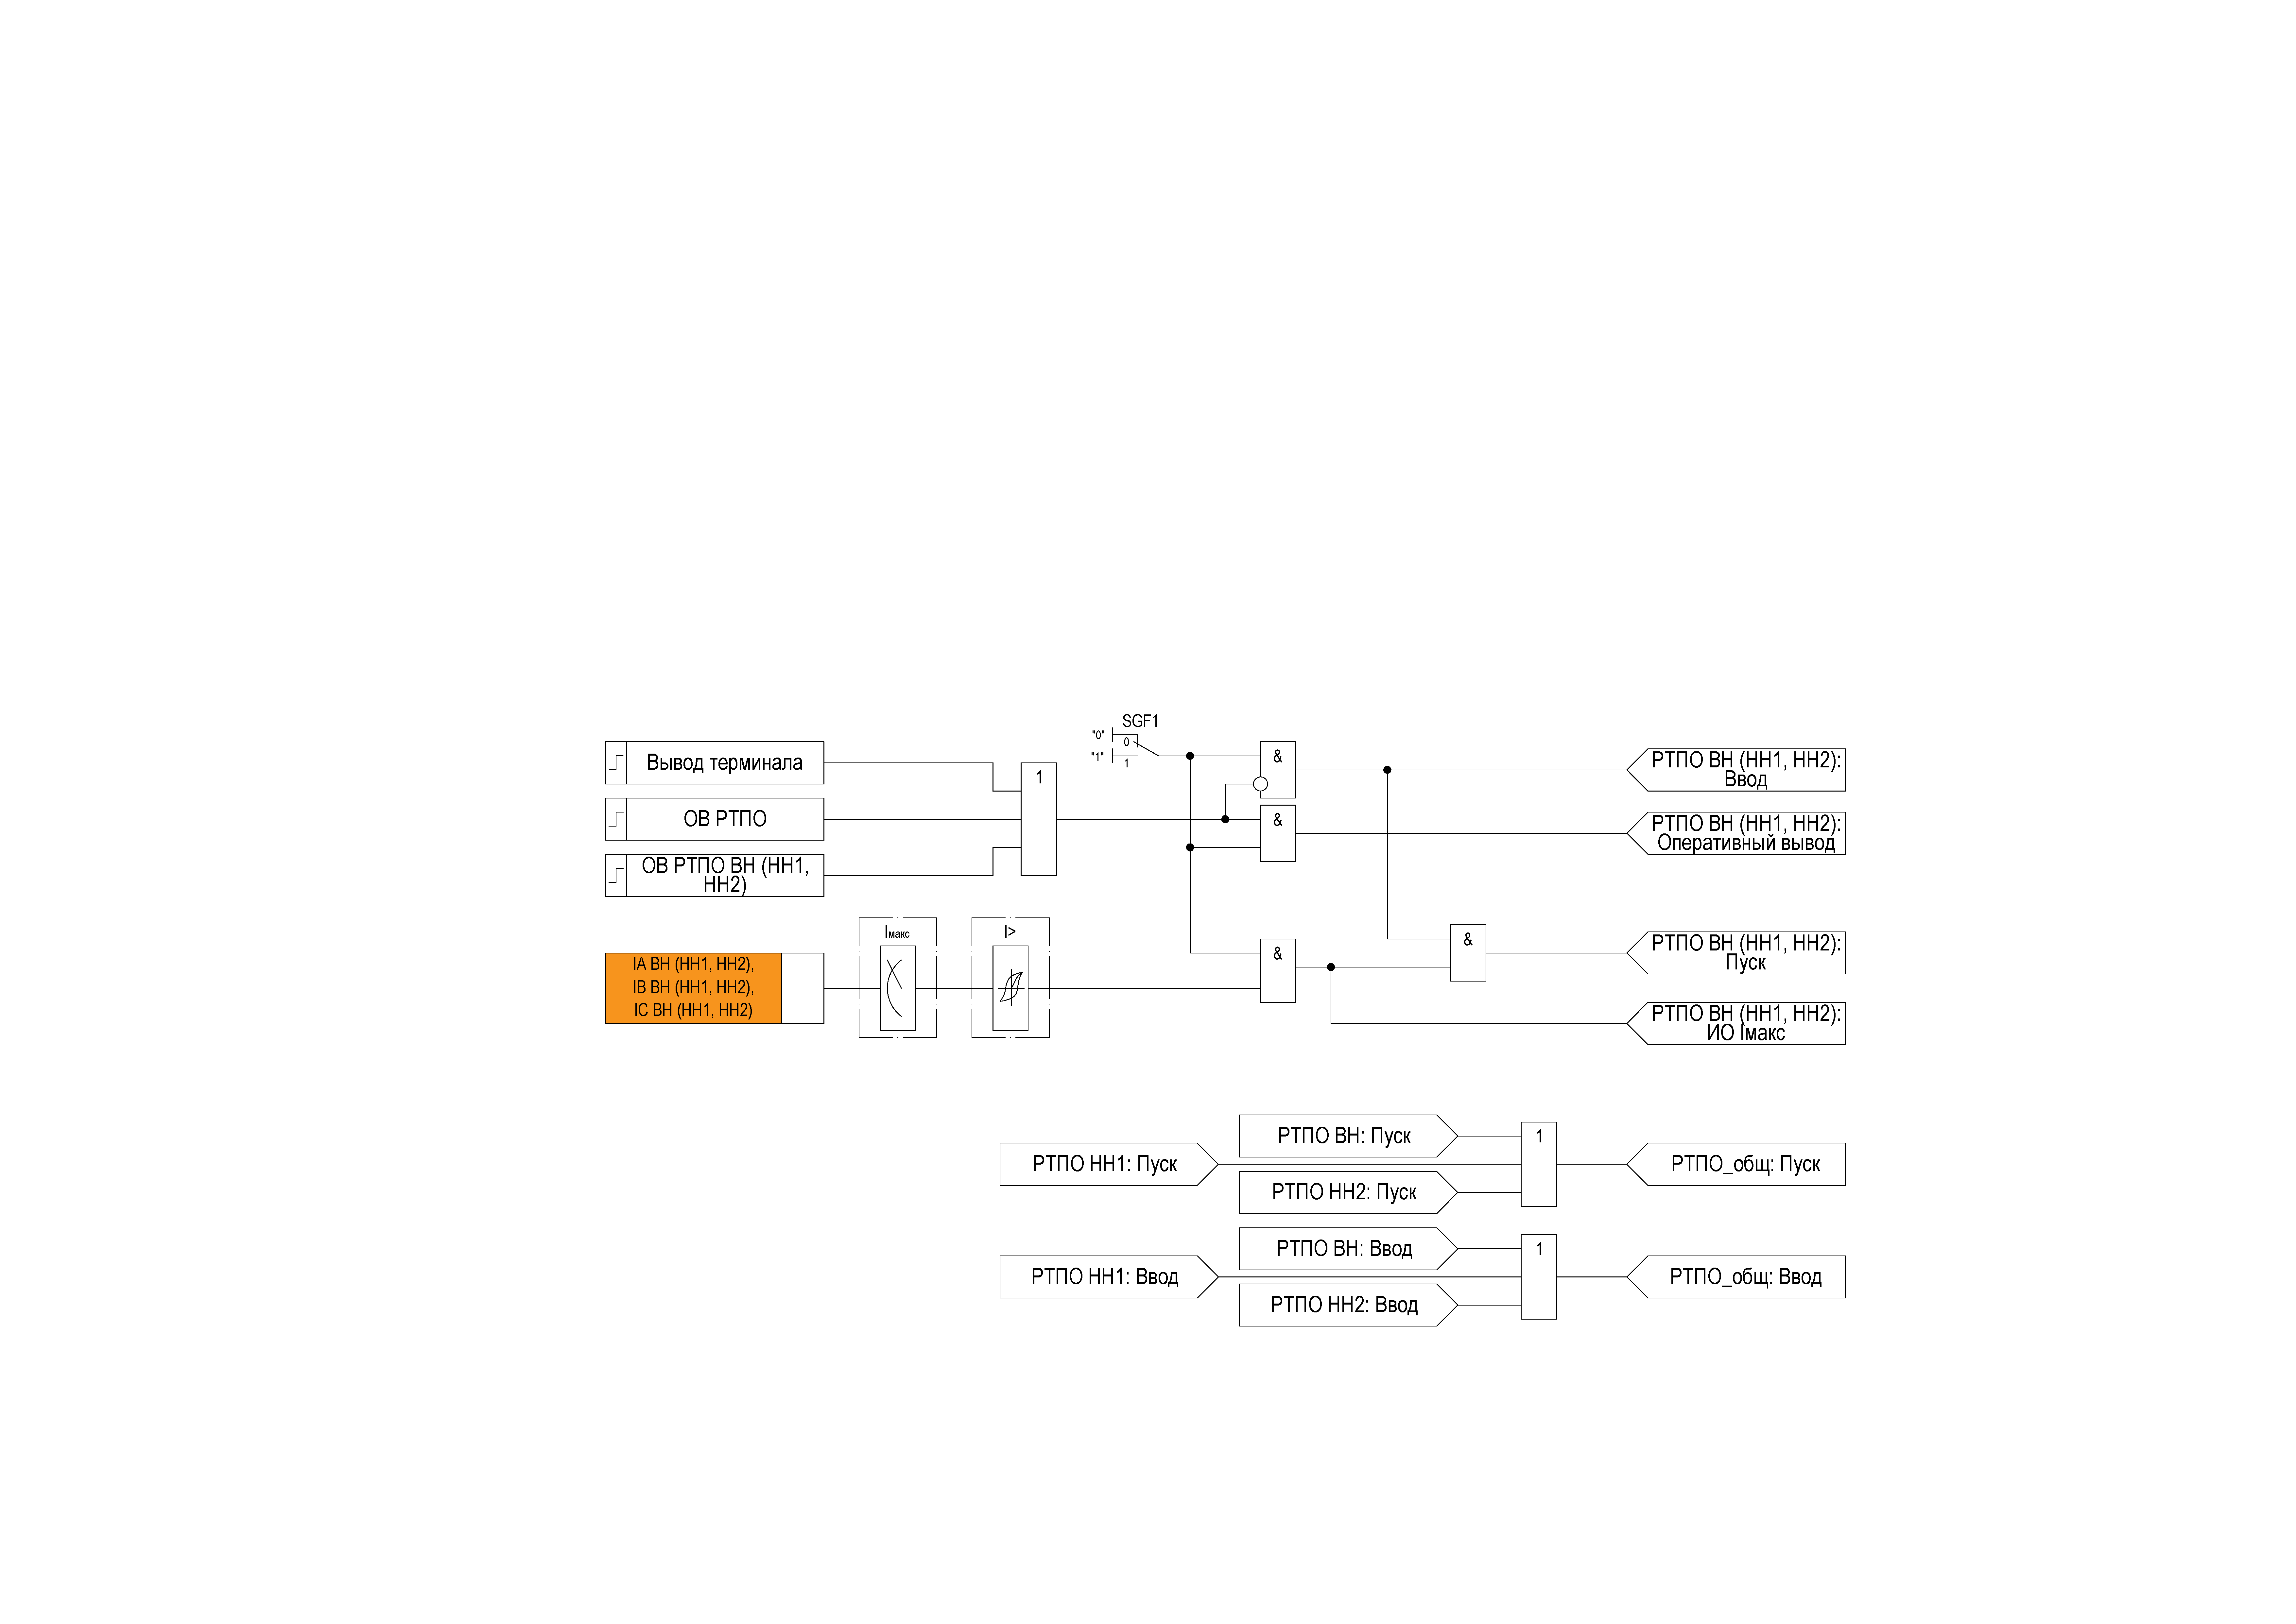
\includegraphics[width=1\textwidth,height=1\textheight,keepaspectratio]{img17.pdf}
\captionof{figure}{Функциональная схема <<РТПО>>}\label{rtpo:img1}
\end{figure}

\end{enumerate}
\FloatBarrier % Все float'ы ДО этой строки будут размещены здесь.

\needspace{4\baselineskip}
\color{uniblue}{\subsection{Токовый контроль для защиты от дуговых замыканий (ТК ЗДЗ)}}
\color{black}

\begin{enumerate}[label=\arabic{section}.\arabic{subsection}.\arabic*, labelsep=4pt, leftmargin=0pt, itemindent=57pt]

\item
Функция <<ТК ЗДЗ>> служит для формирования сигнала наличия тока через трансформатор для алгоритмов дуговых защит секций НН. 
\item
Ввод функции токового контроля в работу на этапе параметрирования устройства осуществляется программным переключателем SGF1 <<Ввод\_функции>>. Информация о введенной функции отображается выходным сигналом <<ТК ЗДЗ: Ввод>>.
\item
Функция <<ТК ЗДЗ>> может быть выведена из работы оперативно путем активации сигнала <<ОВ ТК ЗДЗ>>, что характеризуется активным состоянием сигнала <<ТК ЗДЗ: Оперативный вывод>> на выходе функции.
\item
Функция <<ТК ЗДЗ>> контролирует повышение любого фазного тока (\textsl{IA, IB, IC}) стороны ВН трансформатора выше заданной уставки, при превышении заданной уставки выдается пусковой сигнал для выдачи в цепи дуговых защит секций НН трансформатора.
\item
В качестве измерительных органов в токовых органах применяются ИО тока максимального действия, принцип работы которых заключается в пофазном сравнении действующего значения основной гармоники тока с уставкой срабатывания. Коэффициент возврата порогового элемента равен 0,95.

\item
Алгоритм работы функции <<ТК ЗДЗ>> выполнен в соответствии с рисунком \ref{tkzdz:img1}. В таблице \ref{tkzdz:tbl1} приведены параметры, необходимые для настройки функции <<ТК ЗДЗ>>.

\vspace{3mm}
\begin{figure}[!h]
\centering
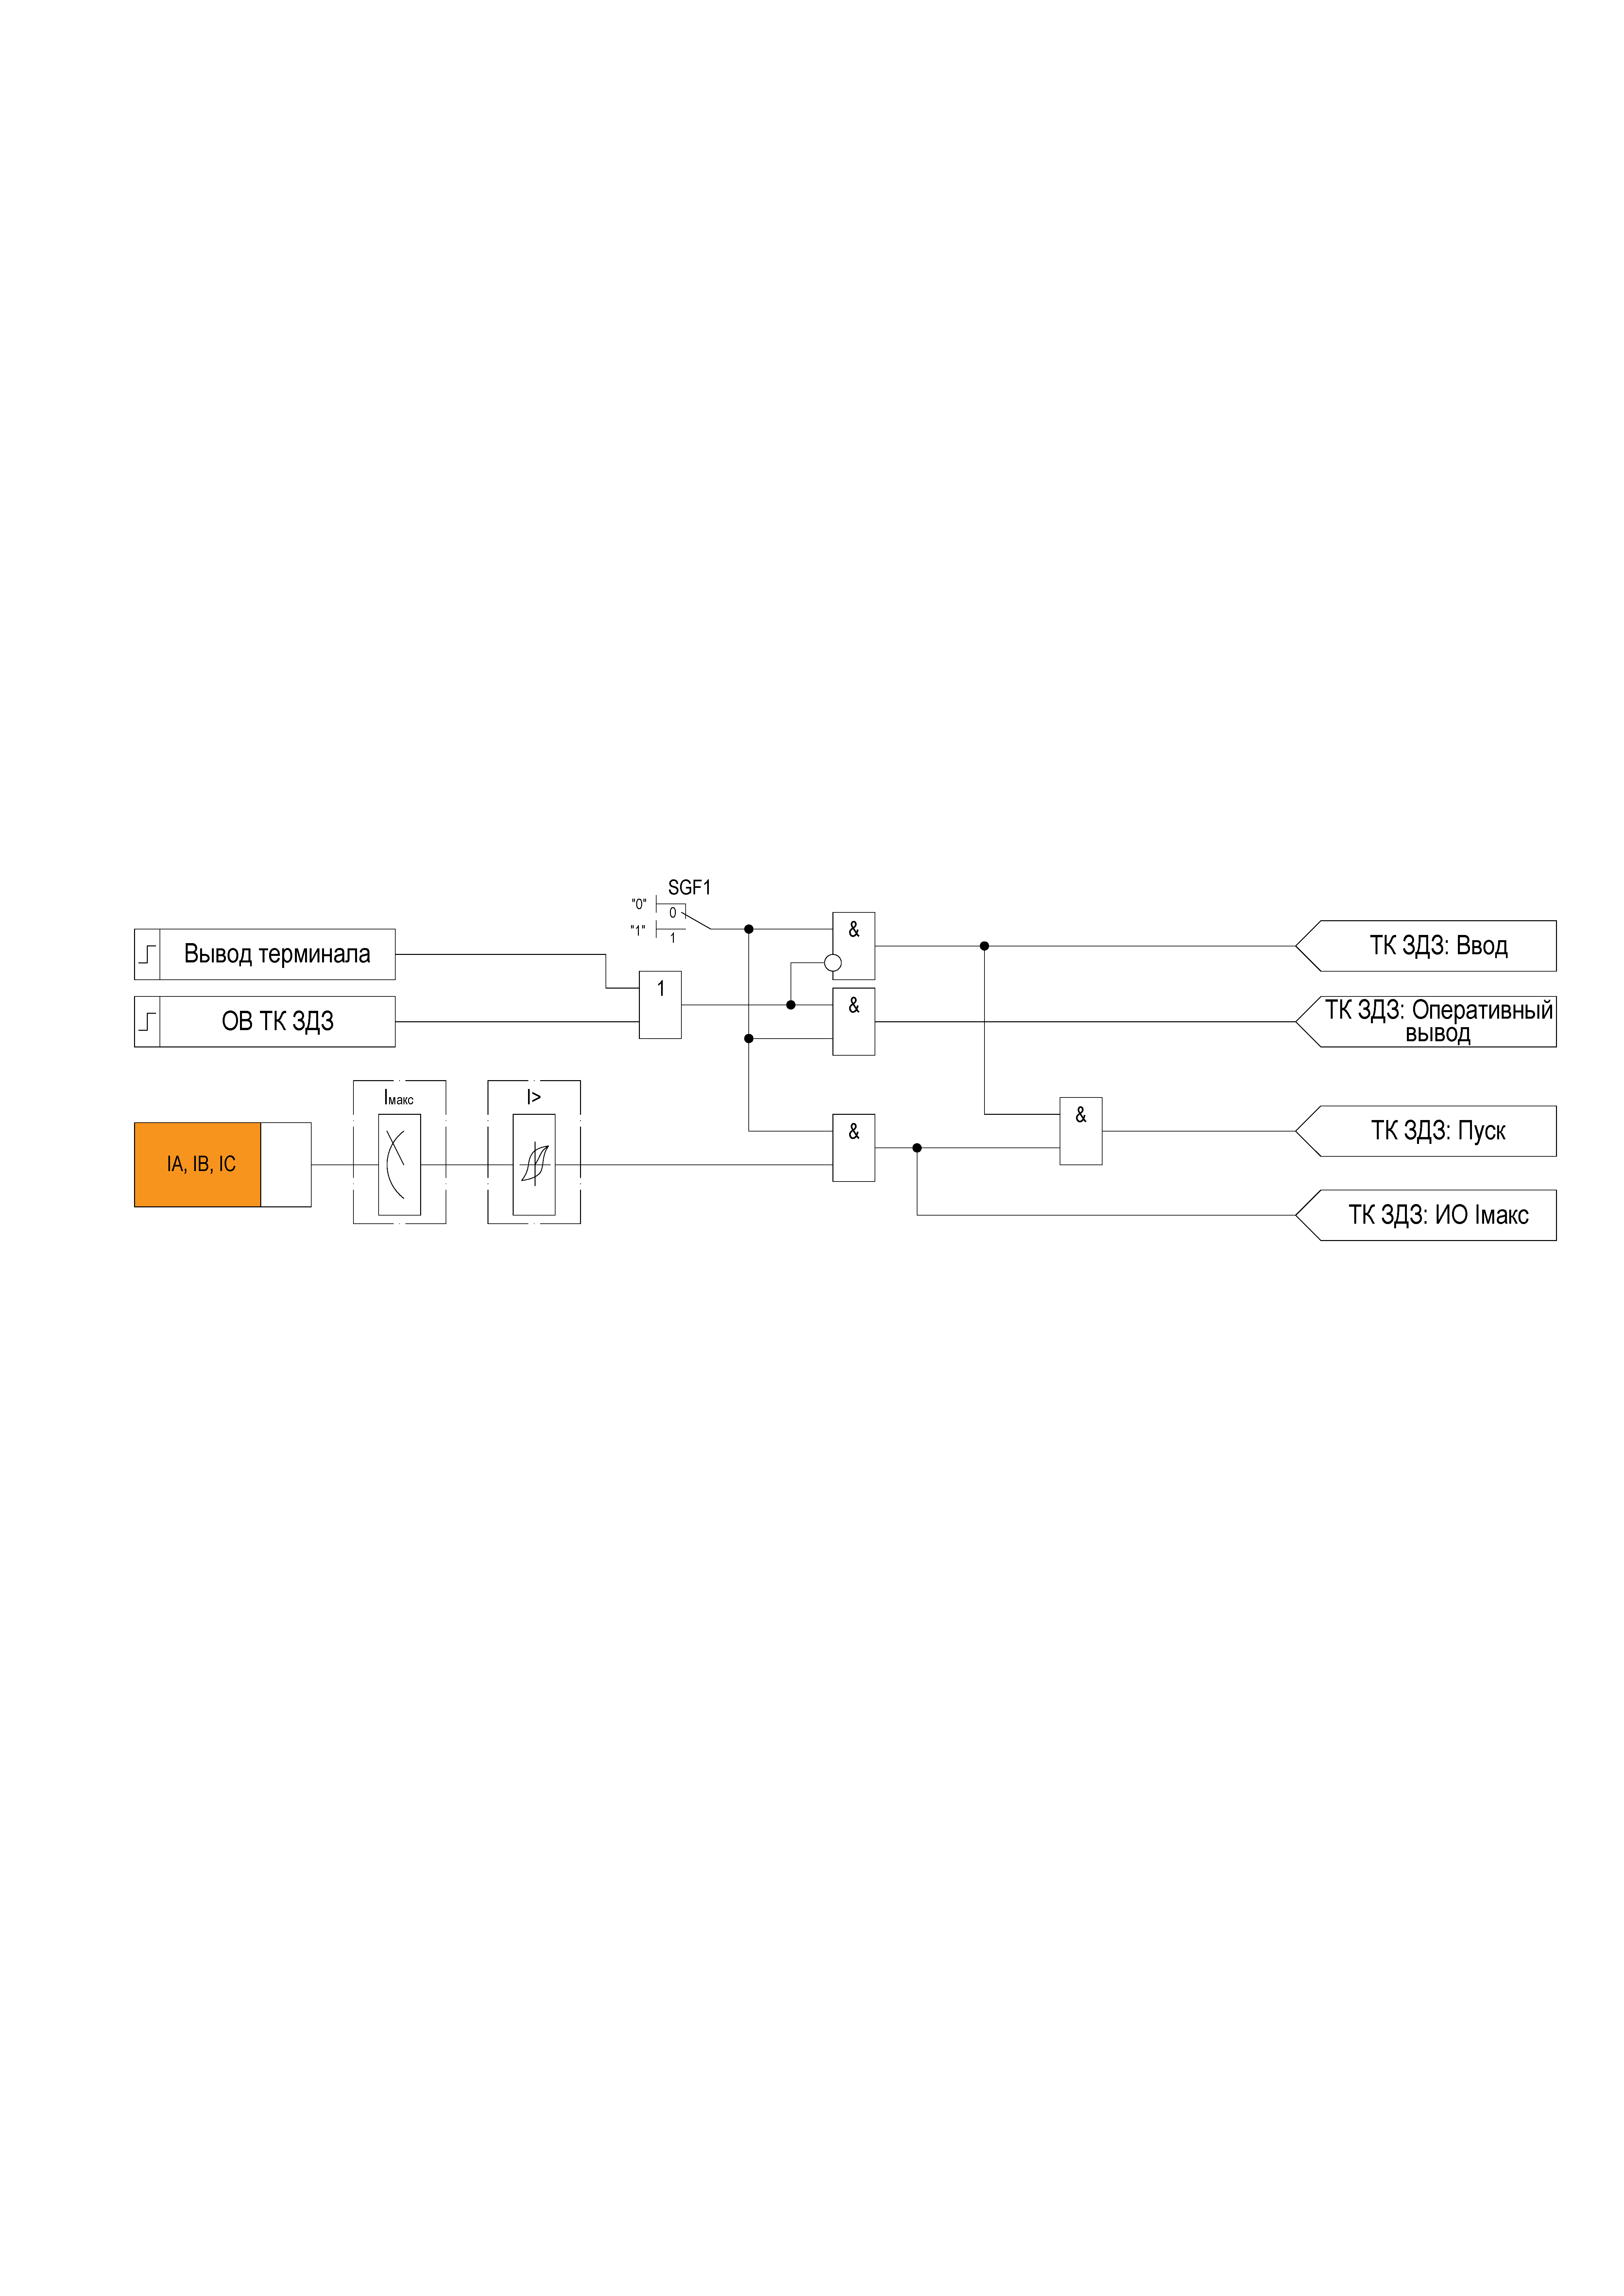
\includegraphics[width=1\textwidth,height=1\textheight,keepaspectratio]{img18.pdf}
\captionof{figure}{Функциональная схема <<ТК ЗДЗ>>}\label{tkzdz:img1}
\end{figure}

\small
\begin{longtable}{|>{\centering\arraybackslash}m{5.3cm}|>{\centering\arraybackslash}m{3.3cm}|>{\centering\arraybackslash}m{4.2cm}|>{\centering\arraybackslash}m{1.8cm}|>{\centering\arraybackslash}m{1cm}|}
\caption{Параметры для настройки функции <<ТК ЗДЗ>>\hfill\vspace{-0.5\baselineskip}}\label{tkzdz:tbl1}\\ 
\hline
\rowcolor{gray!30}
Параметр (Параметр на ИЧМ) & Условное обозначение на схеме & Значение/ Диапазон & Единица измерения & Шаг \\ 
\hline
\endfirsthead
\caption*{\hspace{3pt}\emph{Продолжение таблицы \ref{tkzdz:tbl1}\hfill\vspace{-0.5\baselineskip}}} \\ % сделано по ГОСТ 2.105 п.6.8.7
\hline
\rowcolor{gray!30}
Параметр (Параметр на ИЧМ) & Условное обозначение на схеме & Значение/ Диапазон & Единица измерения & Шаг \\ 
\endhead
\endfoot
\endlastfoot
\centering Ввод функции в работу (Ввод\_функции) & \centering SGF1 & \centering 0 = Не предусмотрено\\1 = Предусмотрено & \centering -- & \centering \arraybackslash -- \\
\hline
\centering Ток срабатывания (Iср) & \centering I$>$ & \centering 0,10 ... 30,00 & \centering о.е. & \centering \arraybackslash 0,01 \\
\hline
\end{longtable}
\normalsize
\end{enumerate}
\FloatBarrier % Все float'ы ДО этой строки будут размещены здесь.

\needspace{4\baselineskip}
\color{uniblue}{\subsection{Токовый орган блокировки РПН (ТО РПН)}}
\color{black}

\begin{enumerate}[label=\arabic{section}.\arabic{subsection}.\arabic*, labelsep=4pt, leftmargin=0pt, itemindent=57pt]

\item
Токовый орган блокировки РПН служит для формирования сигнала превышения допустимого тока через устройство РПН трансформатора для блокировки переключения устройства РПН.
\item
Ввод функции в работу на этапе параметрирования устройства осуществляется программным переключателем SGF1 <<Ввод\_функции>>. Информация о введенной функции отображается выходным сигналом <<ТО РПН: Ввод>>.
\item
Функция <<ТО РПН>> может быть выведена из работы оперативно путем активации сигнала <<ОВ ТО РПН>>, что характеризуется активным состоянием сигнала <<ТО РПН: Оперативный вывод>> на выходе функции.
\item
Функция <<ТО РПН>> контролирует повышение любого фазного тока (\textsl{IA, IB, IC}) стороны ВН трансформатора выше заданной уставки, при превышении заданной уставки выдается пусковой сигнал для блокировки переключений РПН трансформатора.
\item
В качестве измерительных органов в токовых органах применяются ИО тока максимального действия, принцип работы которых заключается в пофазном сравнении действующего значения основной гармоники тока с уставкой срабатывания. Коэффициент возврата порогового элемента равен 0,95.

\item
Алгоритм работы <<ТО РПН>> выполнен в соответствии с рисунком \ref{torpn:img1}. В таблице \ref{torpn:tbl1} приведены параметры, необходимые для настройки функции <<ТО РПН>>.

\vspace{3mm}
\begin{figure}[!h]
\centering
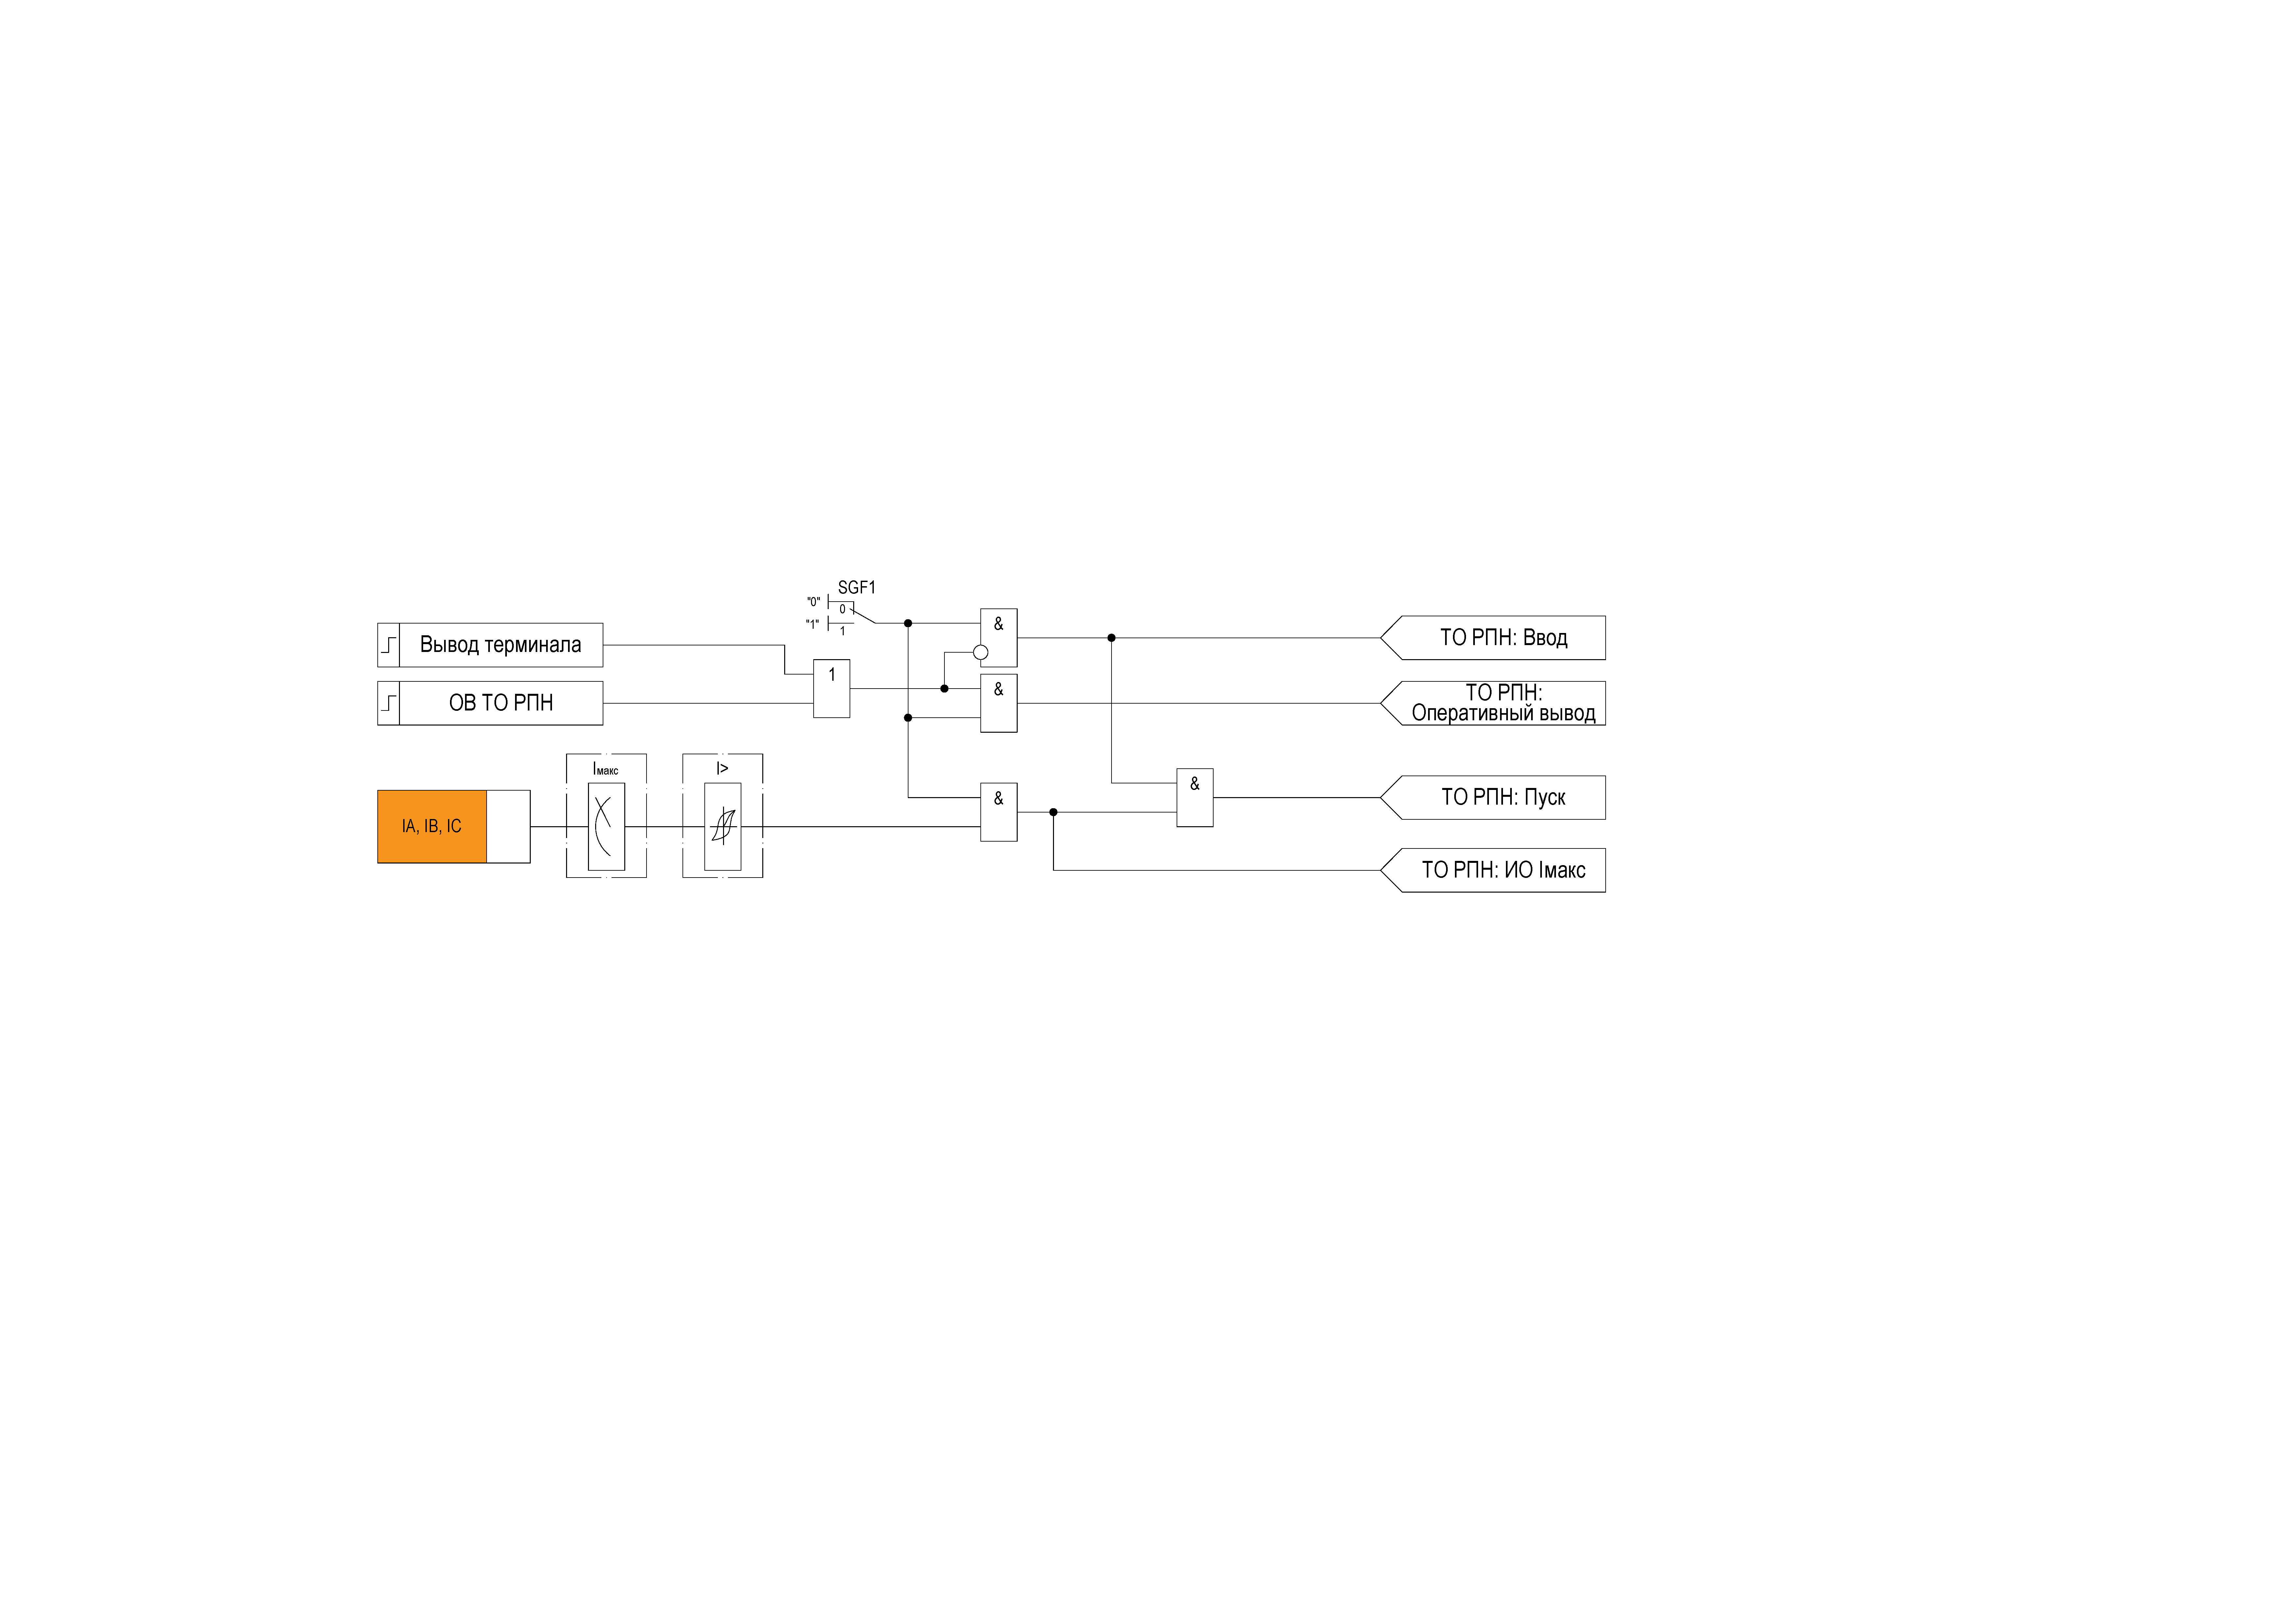
\includegraphics[width=1\textwidth,height=1\textheight,keepaspectratio]{img19.pdf}
\captionof{figure}{Функциональная схема <<ТО РПН>>}\label{torpn:img1}
\end{figure}

\small
\begin{longtable}{|>{\centering\arraybackslash}m{5.3cm}|>{\centering\arraybackslash}m{3.3cm}|>{\centering\arraybackslash}m{4.2cm}|>{\centering\arraybackslash}m{1.8cm}|>{\centering\arraybackslash}m{1cm}|}
\caption{Параметры для настройки функции <<ТО РПН>>\hfill\vspace{-0.5\baselineskip}}\label{torpn:tbl1}\\ 
\hline
\rowcolor{gray!30}
Параметр (Параметр на ИЧМ) & Условное обозначение на схеме & Значение/ Диапазон & Единица измерения & Шаг \\ 
\hline
\endfirsthead
\caption*{\hspace{3pt}\emph{Продолжение таблицы \ref{torpn:tbl1}\hfill\vspace{-0.5\baselineskip}}} \\ % сделано по ГОСТ 2.105 п.6.8.7
\hline
\rowcolor{gray!30}
Параметр (Параметр на ИЧМ) & Условное обозначение на схеме & Значение/ Диапазон & Единица измерения & Шаг \\ 
\endhead
\endfoot
\endlastfoot
\centering Ввод функции в работу (Ввод\_функции) & \centering SGF1 & \centering 0 = Не предусмотрено\\1 = Предусмотрено & \centering -- & \centering \arraybackslash -- \\
\hline
\centering Ток срабатывания (Iср) & \centering I$>$ & \centering 0,10 ... 30,00 & \centering о.е. & \centering \arraybackslash 0,01 \\
\hline
\end{longtable}
\normalsize

\end{enumerate}
\FloatBarrier % Все float'ы ДО этой строки будут размещены здесь.

\needspace{4\baselineskip}
\color{uniblue}{\subsection{Логика отключения при срабатывании отключающего контакта газового реле трансформатора (ЛО ГЗоткл)}}
\color{black}

\begin{enumerate}[label=\arabic{section}.\arabic{subsection}.\arabic*, labelsep=4pt, leftmargin=0pt, itemindent=57pt]

\item
Логика отключения при срабатывании отключающего контакта газового реле трансформатора служит для реализации действия на отключение трансформатора при замыкании отключающего контакта газового реле трансформатора.
\item
Ввод функции в работу на этапе параметрирования устройства осуществляется программным переключателем SGF1 <<Ввод\_функции>>. Информация о введенной функции отображается выходным сигналом <<ЛО ГЗоткл / ЛО: Ввод>>.
\item
Функция <<ЛО ГЗоткл>> может быть выведена из работы оперативно путем активации сигнала <<ОВ ГЗоткл>>, что характеризуется активным состоянием сигнала <<ЛО ГЗоткл / ЛО: Оперативный вывод>> на выходе функции. 
\item
При активном состоянии входного сигнала <<ГЗоткл~на~сигн>> действие отключающей логики переводится на сигнал.
\item
В алгоритме предусмотрена возможность блокировки срабатывания на отключение при приеме сигнала <<Сраб. КИ ГЗ\_откл>> от внешнего устройства контроля изоляции цепей газового реле и введенном программном переключателе SGF2 <<Блок\_от\_НИ>>. Для отстройки от кратковременных неисправностей в цепях газовой защиты может быть введена дополнительная выдержка времени таймера T1 (уставка <<Тбл>>) на прохождение сигнала <<Сраб. КИ ГЗ\_откл>> в логику блокировки. 
Появление сигнала <<Сраб. КИ ГЗ\_откл>> фиксируется элементом памяти, сброс блокировки осуществляется от сигнала <<Сброс>>.
\item
Алгоритм работы <<ЛО~ГЗоткл>> выполнен в соответствии с рисунком \ref{logzotkl:img1}. В таблице \ref{logzotkl:tbl1} приведены параметры, необходимые для настройки функции <<ЛО~ГЗоткл>>.

\small
\begin{longtable}{|>{\centering\arraybackslash}m{5.3cm}|>{\centering\arraybackslash}m{3.3cm}|>{\centering\arraybackslash}m{4.2cm}|>{\centering\arraybackslash}m{1.8cm}|>{\centering\arraybackslash}m{1cm}|}
\caption{Параметры для настройки функции <<ЛО ГЗоткл>>\hfill\vspace{-0.5\baselineskip}}\label{logzotkl:tbl1}\\ 
\hline
\rowcolor{gray!30}
Параметр (Параметр на ИЧМ) & Условное обозначение на схеме & Значение/ Диапазон & Единица измерения & Шаг \\ 
\hline
\endfirsthead
\caption*{\hspace{3pt}\emph{Продолжение таблицы \ref{logzotkl:tbl1}\hfill\vspace{-0.5\baselineskip}}} \\ % сделано по ГОСТ 2.105 п.6.8.7
\hline
\rowcolor{gray!30}
Параметр (Параметр на ИЧМ) & Условное обозначение на схеме & Значение/ Диапазон & Единица измерения & Шаг \\ 
\endhead
\endfoot
\endlastfoot
\centering Ввод функции в работу (Ввод\_функции) & \centering SGF1 & \centering 0 = Не предусмотрено\\1 = Предусмотрено & \centering -- & \centering \arraybackslash -- \\
\hline
\centering Блокировка от низкой изоляции (Блок\_от\_НИ) & \centering SGF2 & \centering 0 = Не предусмотрено\\1 = Предусмотрено & \centering -- & \centering \arraybackslash -- \\
\hline
\centering Выдержка времени срабатывания на блокировку (Тбл) & \centering T1 & \centering 0,00 ... 30,00 & \centering с & \centering \arraybackslash 0,01 \\
\hline
\end{longtable}
\normalsize

\vspace{3mm}
\begin{figure}[H]
\centering
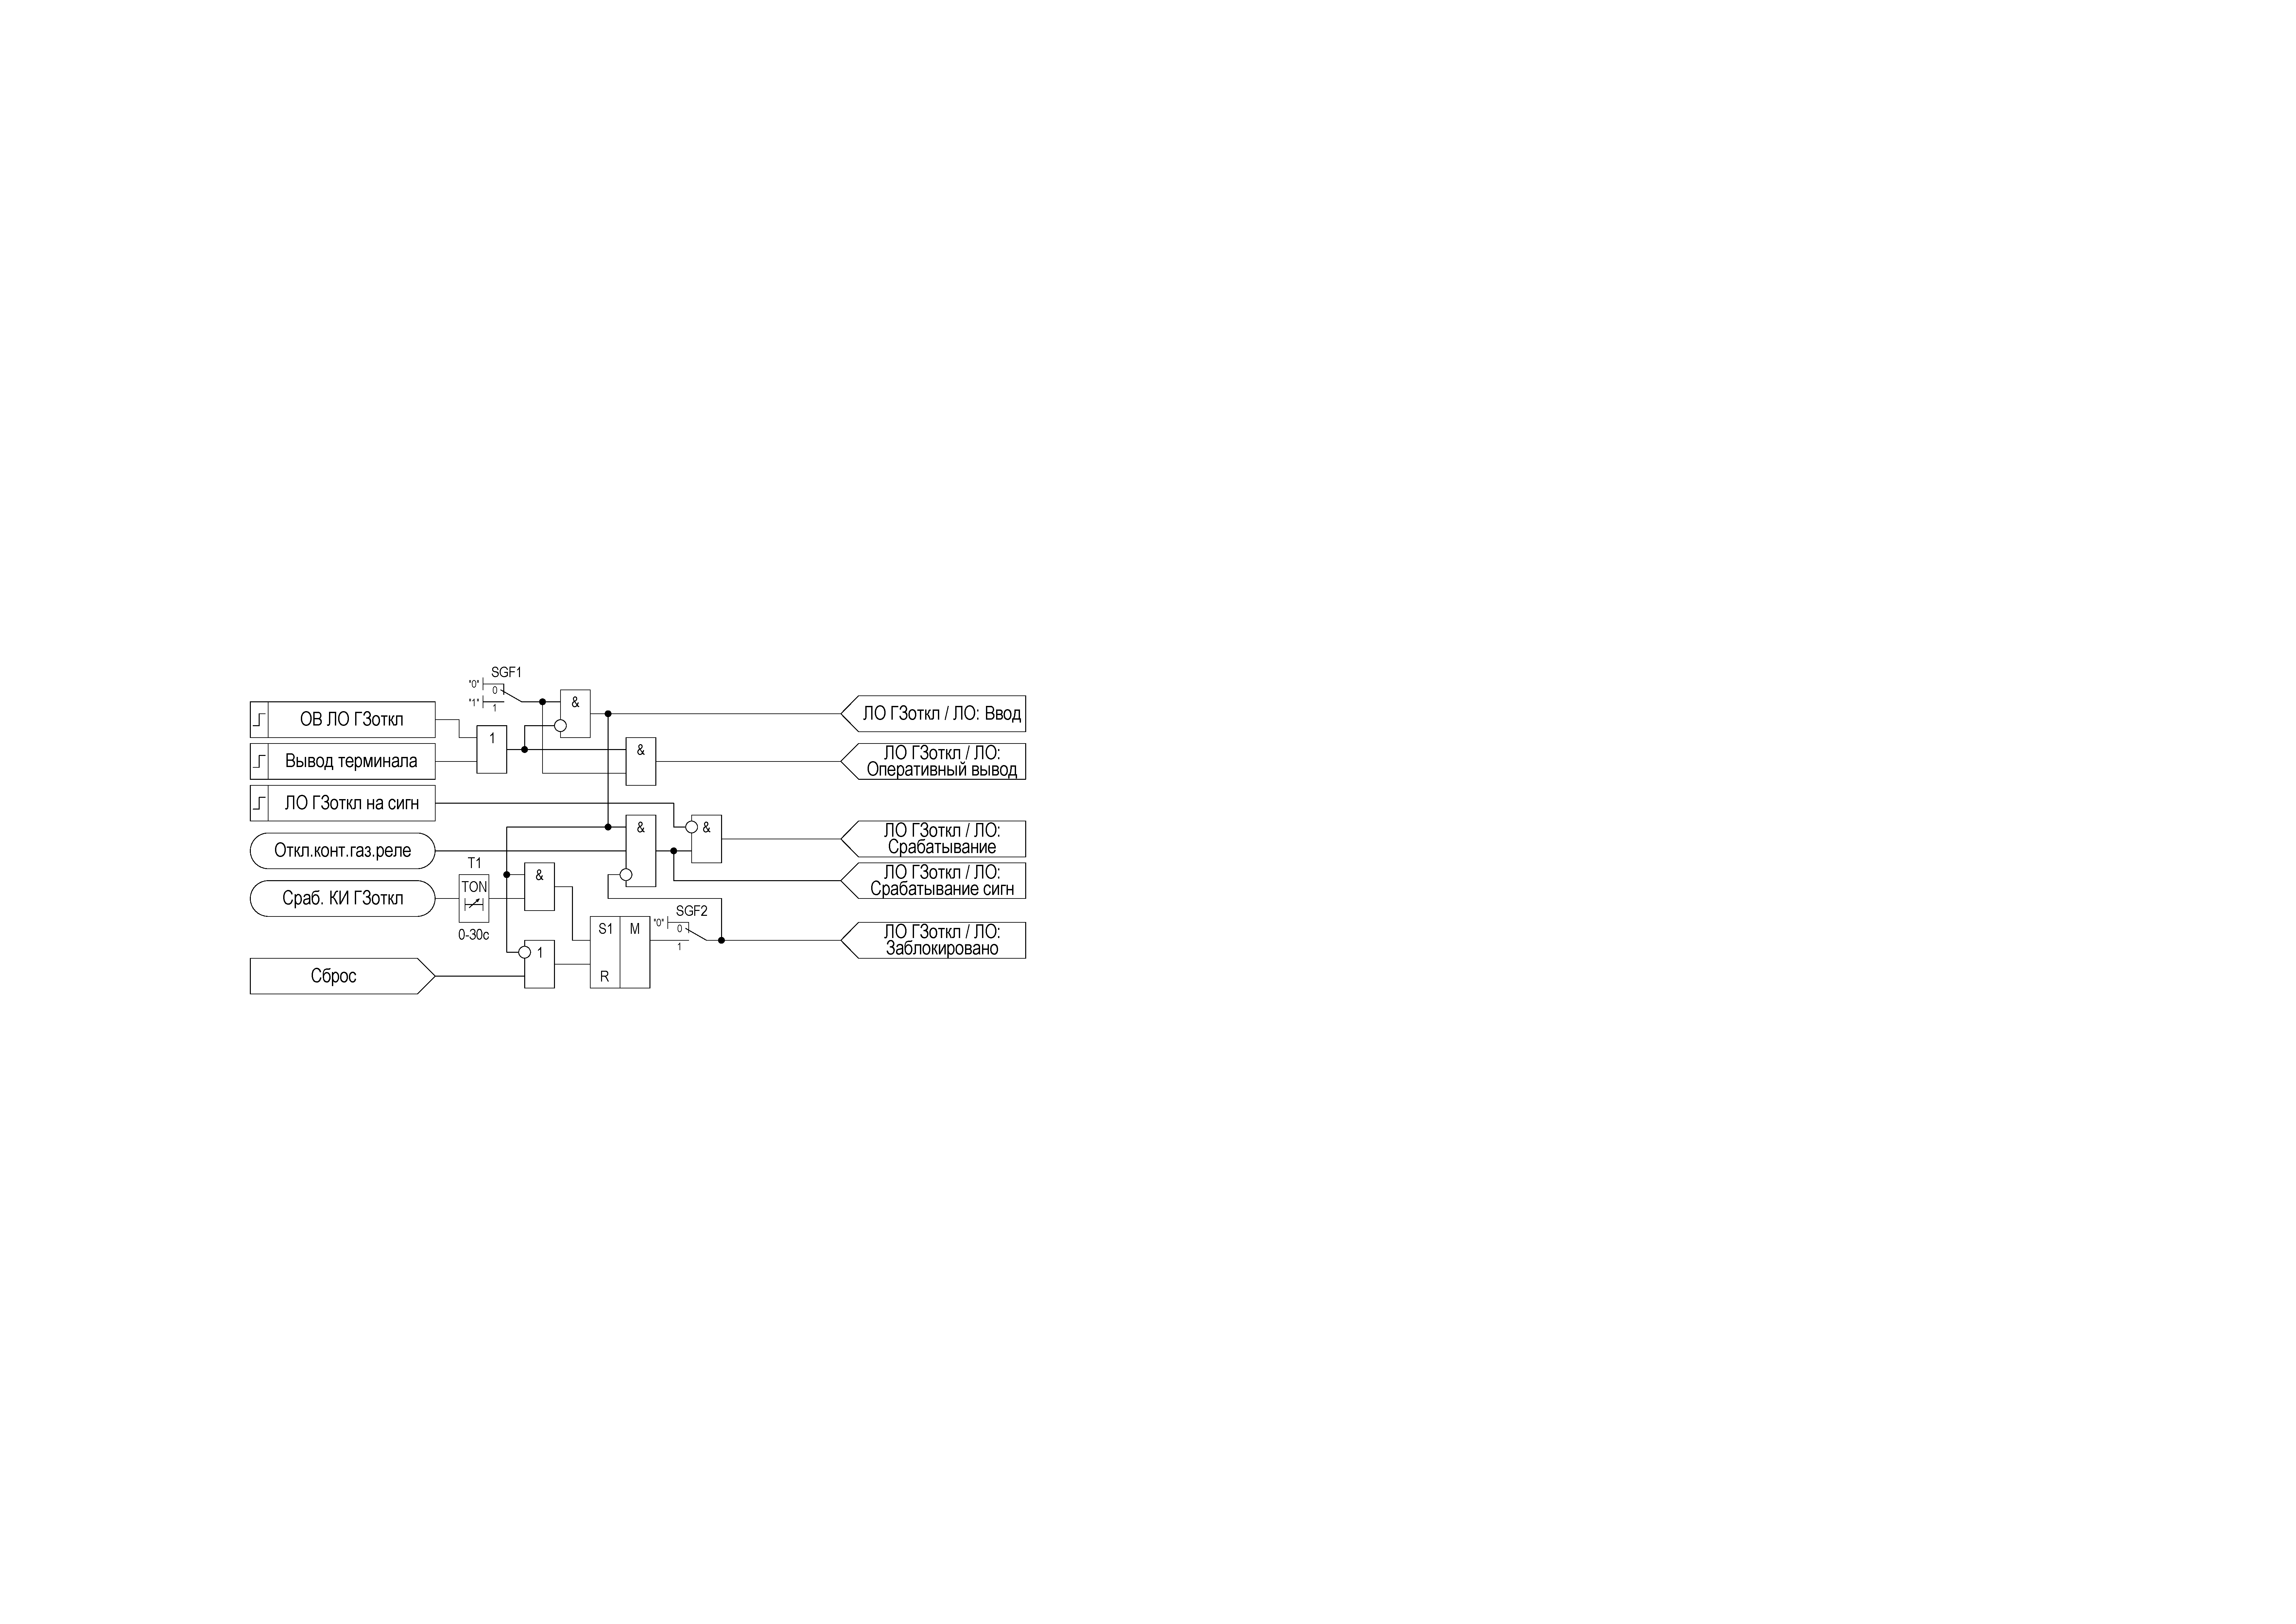
\includegraphics[width=0.95\textwidth,height=0.95\textheight,keepaspectratio]{img20.pdf}
\captionof{figure}{Функциональная схема <<ЛО ГЗоткл>>}\label{logzotkl:img1}
\end{figure}

\end{enumerate}
\FloatBarrier % Все float'ы ДО этой строки будут размещены здесь.


\needspace{4\baselineskip}
\color{uniblue}{\subsection{Логика отключения при срабатывании сигнального контакта газового реле трансформатора (ЛО ГЗсигн)}}
\color{black}

\begin{enumerate}[label=\arabic{section}.\arabic{subsection}.\arabic*, labelsep=4pt, leftmargin=0pt, itemindent=57pt]

\item
Логика отключения при срабатывании сигнального контакта газового реле трансформатора служит для реализации действия на отключение трансформатора при замыкании сигнального контакта газового реле трансформатора. 
\item
Ввод функции в работу на этапе параметрирования устройства осуществляется программным переключателем SGF1 <<Ввод\_функции>>. Информация о введенной функции отображается выходным сигналом <<ЛО ГЗсигн / ЛО: Ввод>>.
\item
Функция <<ЛО ГЗсигн>> может быть выведена из работы оперативно путем активации сигнала <<ОВ ГЗсигн>>, что характеризуется активным состоянием сигнала <<ЛО ГЗсигн / ЛО: Оперативный вывод>> на выходе функции. 
\item
При активном состоянии входного сигнала <<ГЗсигн~на~откл>> действие отключающей логики переводится на отключение.
\item
В алгоритме предусмотрена возможность блокировки срабатывания на отключение при приеме сигнала <<Сраб. КИ ГЗ\_сигн>> от внешнего устройства контроля изоляции цепей газового реле и введенном программном переключателе SGF2 <<Блок\_от\_НИ>>. Для отстройки от кратковременных неисправностей в цепях газовой защиты может быть введена дополнительная выдержка времени таймера T1 (уставка <<Тбл>>) на прохождение сигнала <<Сраб. КИ ГЗ\_сигн>> в логику блокировки. 
Появление сигнала <<Сраб. КИ ГЗ\_сигн>> фиксируется элементом памяти, сброс блокировки осуществляется от сигнала <<Сброс>>.
\item
Алгоритм работы <<ЛО~ГЗсигн>> выполнен в соответствии с рисунком \ref{logzsign:img1}. В таблице \ref{logzsign:tbl1} приведены параметры, необходимые для настройки функции <<ЛО~ГЗсигн>>.

\small
\begin{longtable}{|>{\centering\arraybackslash}m{5.3cm}|>{\centering\arraybackslash}m{3.3cm}|>{\centering\arraybackslash}m{4.2cm}|>{\centering\arraybackslash}m{1.8cm}|>{\centering\arraybackslash}m{1cm}|}
\caption{Параметры для настройки функции <<ЛО ГЗсигн>>\hfill\vspace{-0.5\baselineskip}}\label{logzsign:tbl1}\\ 
\hline
\rowcolor{gray!30}
Параметр (Параметр на ИЧМ) & Условное обозначение на схеме & Значение/ Диапазон & Единица измерения & Шаг \\ 
\hline
\endfirsthead
\caption*{\hspace{3pt}\emph{Продолжение таблицы \ref{logzsign:tbl1}\hfill\vspace{-0.5\baselineskip}}} \\ % сделано по ГОСТ 2.105 п.6.8.7
\hline
\rowcolor{gray!30}
Параметр (Параметр на ИЧМ) & Условное обозначение на схеме & Значение/ Диапазон & Единица измерения & Шаг \\ 
\endhead
\endfoot
\endlastfoot
\centering Ввод функции в работу (Ввод\_функции) & \centering SGF1 & \centering 0 = Не предусмотрено\\1 = Предусмотрено & \centering -- & \centering \arraybackslash -- \\
\hline
\centering Выдержка времени срабатывания на блокировку (Тбл) & \centering T1 & \centering 0,00 ... 30,00 & \centering с & \centering \arraybackslash 0,01 \\
\hline
\centering Блокировка от низкой изоляции (Блок\_от\_НИ) & \centering SGF2 & \centering 0 = Не предусмотрено\\1 = Предусмотрено & \centering -- & \centering \arraybackslash -- \\
\hline
\end{longtable}
\normalsize

\vspace{3mm}
\begin{figure}[!h]
\centering
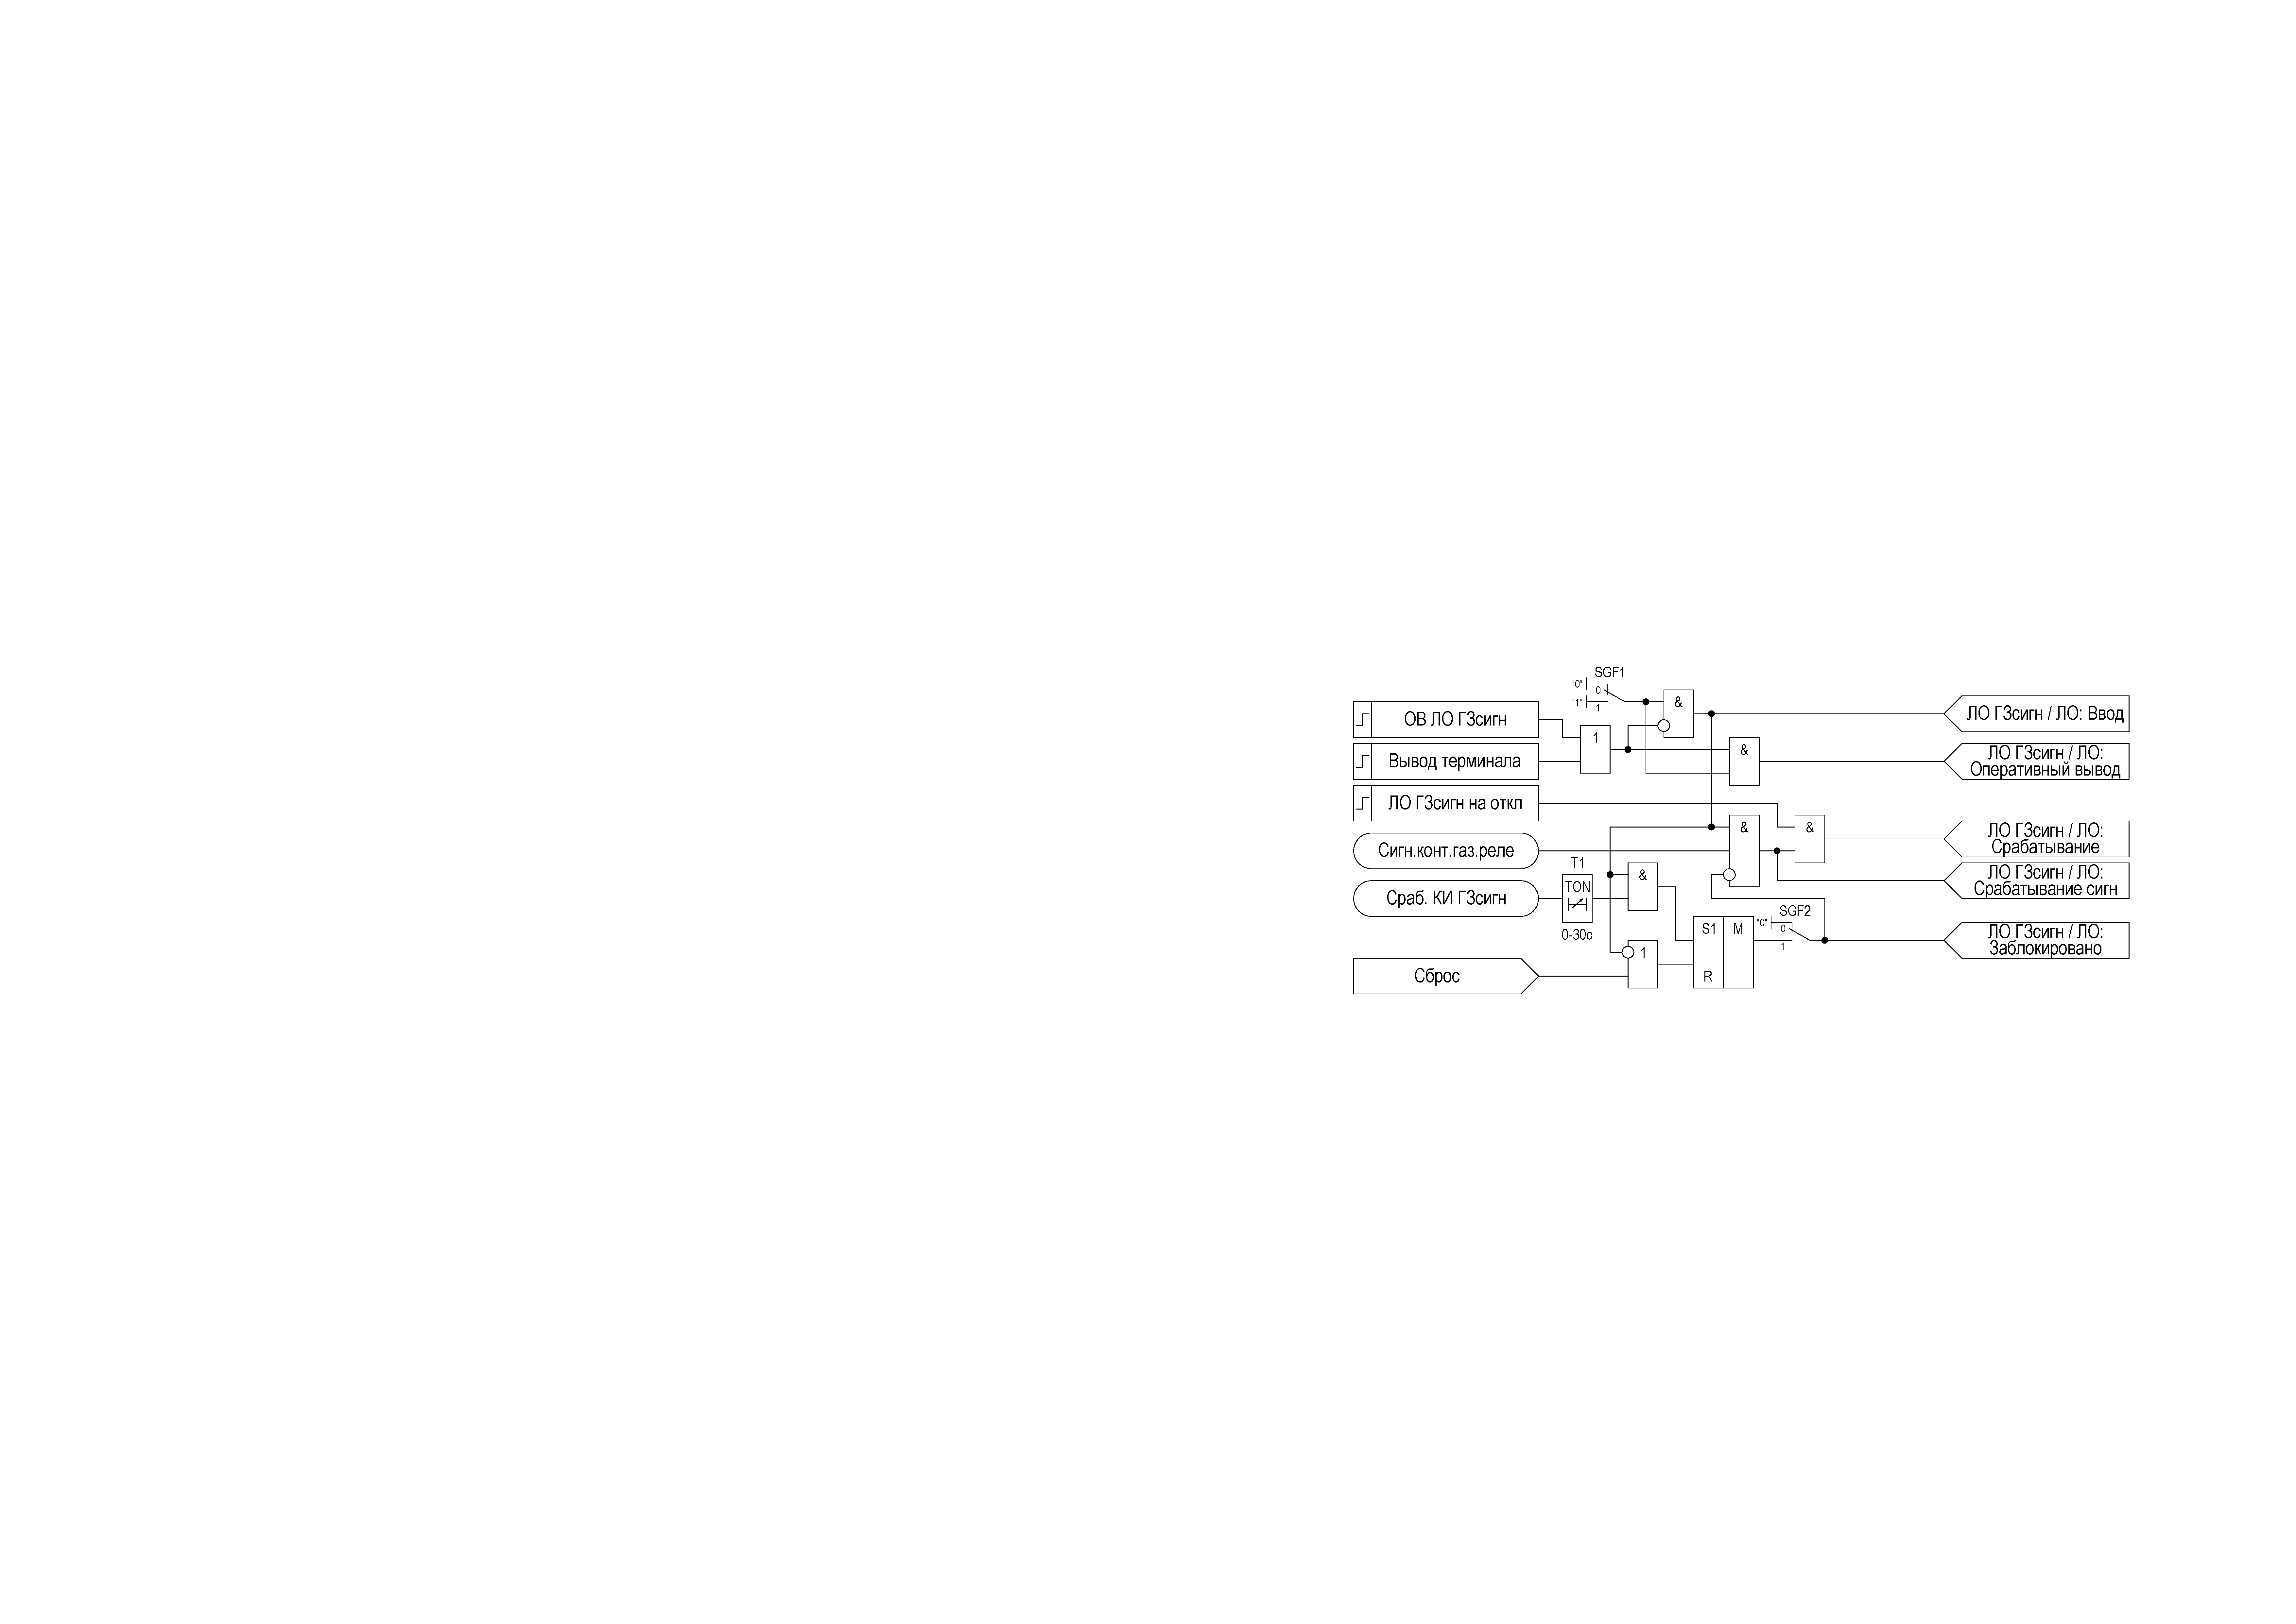
\includegraphics[width=0.95\textwidth,height=0.95\textheight,keepaspectratio]{img21.pdf}
\captionof{figure}{Функциональная схема <<ЛО ГЗсигн>>}\label{logzsign:img1}
\end{figure}

\end{enumerate}
\FloatBarrier % Все float'ы ДО этой строки будут размещены здесь.
\needspace{4\baselineskip}
\color{uniblue}{\subsection{Логика отключения при срабатывании струйного реле РПН трансформатора (ЛО~ГЗ~РПН)}}
\color{black}

\begin{enumerate}[label=\arabic{section}.\arabic{subsection}.\arabic*, labelsep=4pt, leftmargin=0pt, itemindent=57pt]

\item
Логика отключения при срабатывании струйного реле РПН трансформатора служит для реализации действия на отключение трансформатора при замыкании контакта струйного реле РПН трансформатора. 
\item
Ввод функции в работу на этапе параметрирования устройства осуществляется программным переключателем SGF1 <<Ввод\_функции>>. Информация о введенной функции отображается выходным сигналом <<ЛО ГЗ РПН / ЛО: Ввод>>.
\item
Функция <<ЛО~ГЗ~РПН>> может быть выведена из работы оперативно путем активации сигнала <<ОВ~ГЗ~РПН>>, что характеризуется активным состоянием сигнала <<ЛО ГЗ РПН / ЛО: Оперативный вывод>> на выходе функции. 
\item
При активном состоянии входного сигнала <<ГЗ~РПН~на~сигн>> действие отключающей логики переводится на сигнал.
\item
В алгоритме предусмотрена возможность блокировки срабатывания на отключение при приеме сигнала <<Сраб. КИ ГЗ\_РПН>> от внешнего устройства контроля изоляции цепей струйного реле и введенном программном переключателе SGF2 <<Блок\_от\_НИ>>. Для отстройки от кратковременных неисправностей в цепях струйного реле может быть введена дополнительная выдержка времени таймера T1 (уставка <<Тбл>>) на прохождение сигнала <<Сраб. КИ ГЗ\_РПН>> в логику блокировки. 
Появление сигнала <<Сраб. КИ ГЗ\_РПН>> фиксируется элементом памяти, сброс блокировки осуществляется от сигнала <<Сброс>>.
\item
Алгоритм работы <<ЛО~ГЗ~РПН>> выполнен в соответствии с рисунком \ref{logzrpn:img1}. В таблице \ref{logzrpn:tbl1} приведены параметры, необходимые для настройки функции <<ЛО~ГЗ~РПН>>.

\small
\begin{longtable}{|>{\centering\arraybackslash}m{5.3cm}|>{\centering\arraybackslash}m{3.3cm}|>{\centering\arraybackslash}m{4.2cm}|>{\centering\arraybackslash}m{1.8cm}|>{\centering\arraybackslash}m{1cm}|}
\caption{Параметры для настройки функции <<ЛО ГЗ РПН>>\hfill\vspace{-0.5\baselineskip}}\label{logzrpn:tbl1}\\ 
\hline
\rowcolor{gray!30}
Параметр (Параметр на ИЧМ) & Условное обозначение на схеме & Значение/ Диапазон & Единица измерения & Шаг \\ 
\hline
\endfirsthead
\caption*{\hspace{3pt}\emph{Продолжение таблицы \ref{logzrpn:tbl1}\hfill\vspace{-0.5\baselineskip}}} \\ % сделано по ГОСТ 2.105 п.6.8.7
\hline
\rowcolor{gray!30}
Параметр (Параметр на ИЧМ) & Условное обозначение на схеме & Значение/ Диапазон & Единица измерения & Шаг \\ 
\endhead
\endfoot
\endlastfoot
\centering Ввод функции в работу (Ввод\_функции) & \centering SGF1 & \centering 0 = Не предусмотрено\\1 = Предусмотрено & \centering -- & \centering \arraybackslash -- \\
\hline
\centering Блокировка от низкой изоляции (Блок\_от\_НИ) & \centering SGF2 & \centering 0 = Не предусмотрено\\1 = Предусмотрено & \centering -- & \centering \arraybackslash -- \\
\hline
\centering Выдержка времени срабатывания на блокировку (Тбл) & \centering T1 & \centering 0,00 ... 30,00 & \centering с & \centering \arraybackslash 0,01 \\
\hline
\end{longtable}
\normalsize

\vspace{3mm}
\begin{figure}[!h]
\centering
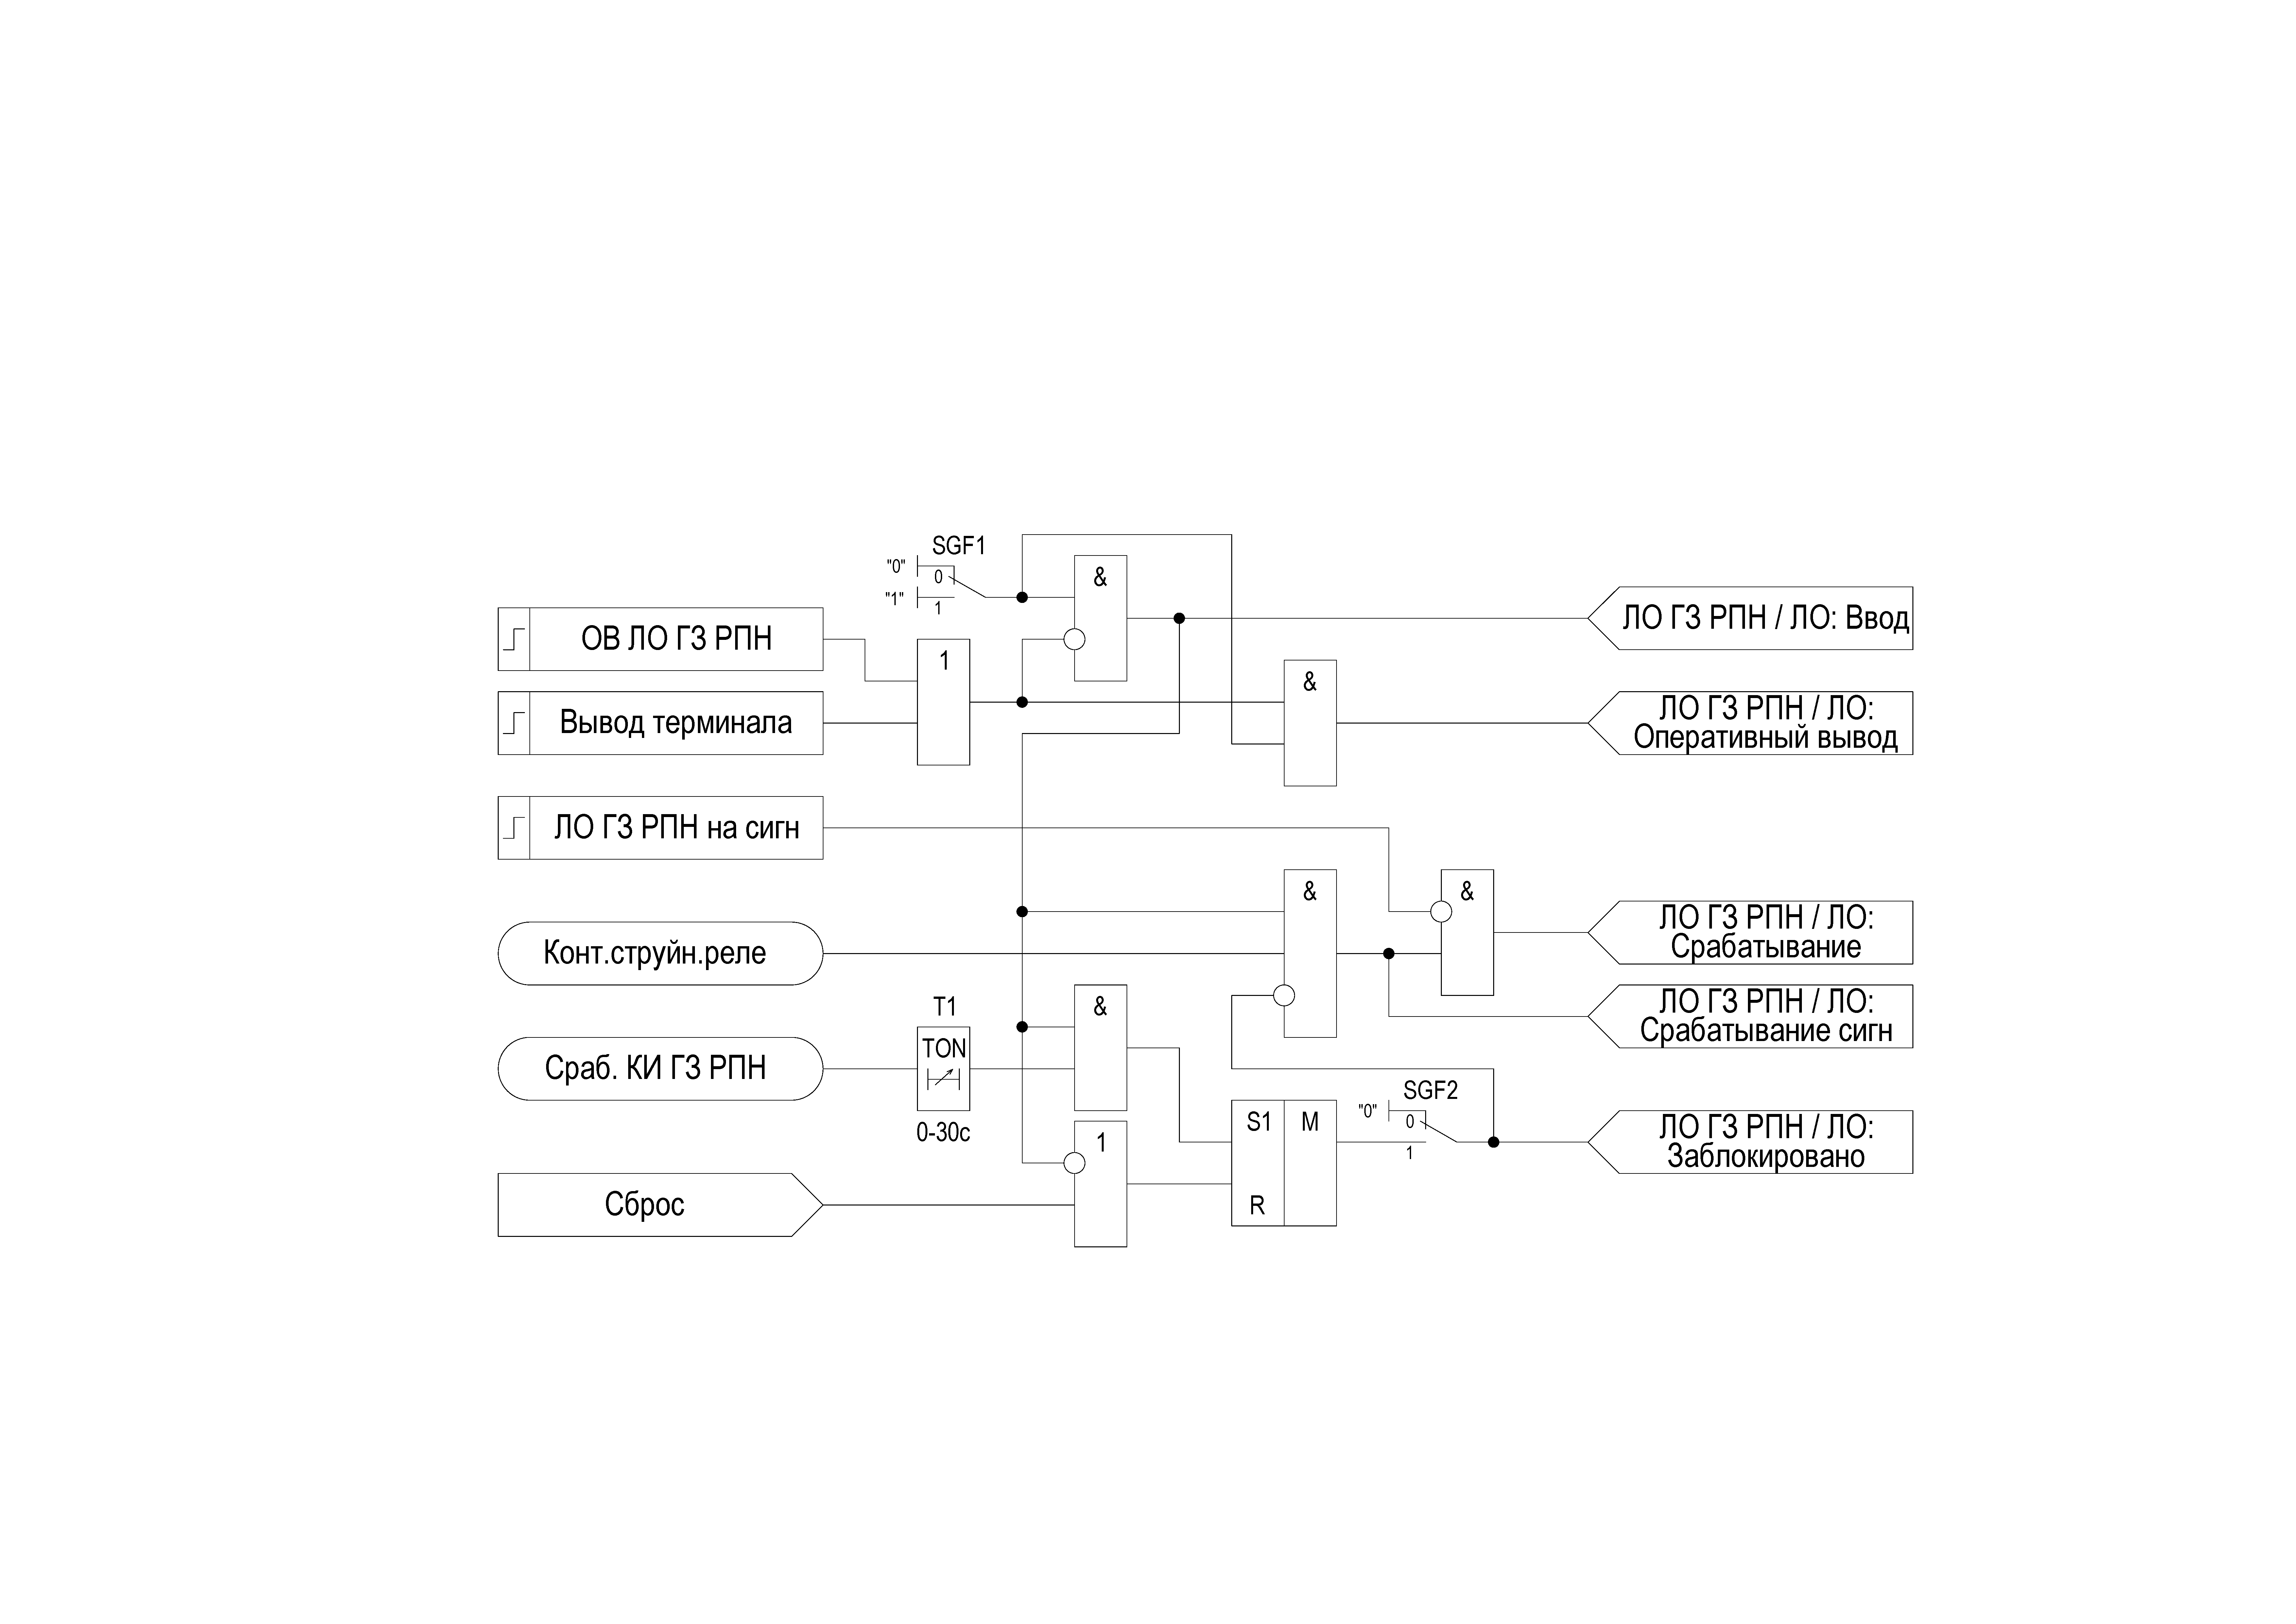
\includegraphics[width=0.95\textwidth,height=0.95\textheight,keepaspectratio]{img22.pdf}
\captionof{figure}{Функциональная схема <<ЛО~ГЗ~РПН>>}\label{logzrpn:img1}
\end{figure}

\end{enumerate}
\FloatBarrier % Все float'ы ДО этой строки будут размещены здесь.
\needspace{4\baselineskip} 
\color{uniblue}{\subsection{\sloppy Логика отключения при срабатывании технологических защит \mbox{трансформатора} (ЛО ТЗ)}}
\color{black}


\begin{enumerate}[label=\arabic{section}.\arabic{subsection}.\arabic{enumi}, labelsep=4pt, leftmargin=0pt, itemindent=57pt, itemsep=0pt, parsep=5pt] % если что можно крутить itemsep

\item Общие сведения

\begin{enumerate}[label=\arabic{section}.\arabic{subsection}.\arabic{enumi}.\arabic*, labelsep=4pt, leftmargin=0em, itemindent=65pt, parsep=0pt]   

\item
Логика отключения при срабатывании технологических защит служит для реализации действия на отключение трансформатора при срабатывании датчиков технологических защит.
\item
Функциональный блок <<ЛО~ТЗ>> может быть выведен из работы оперативно путем активации сигнала <<ОВ~ЛО~ТЗ>>.
\item
В функциональном блоке реализована возможность приема следующих аварийных сигналов от датчиков технологических защит:
\begin{itemize}
\item аварийная температура масла для функции <<ЛО ДТм>>;
\item аварийная температура обмотки для функции <<ЛО ДТо>>;
\item срабатывание реле давления для функции <<ЛО РД>>.
\end{itemize}

\item
В таблице \ref{lotz:tbl1} приведены параметры, необходимые для настройки функций в составе функционального блока <<ЛО ТЗ>>.
\small
\begin{longtable}{|>{\centering\arraybackslash}m{5.3cm}|>{\centering\arraybackslash}m{3.3cm}|>{\centering\arraybackslash}m{4.2cm}|>{\centering\arraybackslash}m{1.8cm}|>{\centering\arraybackslash}m{1cm}|}
\caption{Общие параметры для настройки функционального блока <<ЛО ТЗ>>\hfill\vspace{-0.5\baselineskip}}\label{lotz:tbl1}\\ 
\hline
\rowcolor{gray!30}
Параметр (Параметр на ИЧМ) & Условное обозначение на схеме & Значение/ Диапазон & Единица измерения & Шаг \\ 
\hline
\endfirsthead
\caption*{\hspace{3pt}\emph{Продолжение таблицы \ref{lotz:tbl1}\hfill\vspace{-0.5\baselineskip}}} \\ % сделано по ГОСТ 2.105 п.6.8.7
\hline
\rowcolor{gray!30}
Параметр (Параметр на ИЧМ) & Условное обозначение на схеме & Значение/ Диапазон & Единица измерения & Шаг \\ 
\endhead
\endfoot
\endlastfoot
\centering Выдержка времени срабатывания на блокировку (Тбл) & \centering Т1 & \centering 0,00 ... 30,00 & \centering с & \centering \arraybackslash 0,01 \\
\hline
\end{longtable}
\normalsize

\end{enumerate}

\item Логика отключения при срабатывании датчика температуры масла (ЛО ДТм)

\begin{enumerate}[label=\arabic{section}.\arabic{subsection}.\arabic{enumi}.\arabic*, labelsep=4pt, leftmargin=0em, itemindent=65pt, parsep=0pt] 

\item
Логика отключения при срабатывании датчика температуры масла (<<ЛО ДТм>>) служит для реализации действия на отключение трансформатора при достижении аварийного значения температуры масла трансформатора.

\item
Ввод функции в работу на этапе параметрирования устройства осуществляется программным переключателем SGF1 <<Ввод\_функции>>. Информация о введенной функции отображается выходным сигналом <<ЛО ДТм: Ввод>>.
\item
Функция <<ЛО ДТм>> может быть выведена из работы оперативно путем активации сигнала <<ОВ ЛО ДТм>>, что характеризуется активным состоянием сигнала <<ЛО ДТм: Оперативный вывод>> на выходе функции. 
\item
При активном состоянии входного сигнала <<ДТм~на~сигн>> действие отключающей логики переводится на сигнал.
\item
Для формирования сигнала на отключение от <<ЛО ДТм>> при срабатывании контакта датчика температуры масла аварийной ступени (активное состояние входного сигнала <<Авар. t масла>>) необходимо также наличие сигнала срабатывания контакта датчика температуры масла предупредительной ступени (активное состояние входного сигнала <<Повыш. t масла>>), что является дополнительным подтверждающим фактором исправности цепей датчика температуры масла.

\item
В алгоритме предусмотрена возможность блокировки срабатывания на отключение при приеме сигнала <<Сраб. КИ ДТм>> от внешнего устройства контроля изоляции цепей датчика температуры и введенном программном переключателе SGF2 <<Блок\_от\_НИ>>. Для отстройки от кратковременных неисправностей в цепях датчика температуры может быть введена дополнительная выдержка времени таймера T1 (уставка <<Тбл>>) на прохождение сигнала <<Сраб. КИ ДТм>> в логику блокировки. 
Появление сигнала <<Сраб. КИ ДТм>> фиксируется элементом памяти, сброс блокировки осуществляется от сигнала <<Сброс>>.

\item
Алгоритм работы <<ЛО ДТм>> выполнен в соответствии с рисунком \ref{lotzdtm:img1}. В таблице \ref{lotzdtm:tbl1} приведены параметры, необходимые для настройки функции <<ЛО~ДТм>>.

\small
\begin{longtable}{|>{\centering\arraybackslash}m{5.3cm}|>{\centering\arraybackslash}m{3.3cm}|>{\centering\arraybackslash}m{4.2cm}|>{\centering\arraybackslash}m{1.8cm}|>{\centering\arraybackslash}m{1cm}|}
\caption{Параметры для настройки функции <<ЛО ДТм>>\hfill\vspace{-0.5\baselineskip}}\label{lotzdtm:tbl1}\\ 
\hline
\rowcolor{gray!30}
Параметр (Параметр на ИЧМ) & Условное обозначение на схеме & Значение/ Диапазон & Единица измерения & Шаг \\ 
\hline
\endfirsthead
\caption*{\hspace{3pt}\emph{Продолжение таблицы \ref{lotzdtm:tbl1}\hfill\vspace{-0.5\baselineskip}}} \\ % сделано по ГОСТ 2.105 п.6.8.7
\hline
\rowcolor{gray!30}
Параметр (Параметр на ИЧМ) & Условное обозначение на схеме & Значение/ Диапазон & Единица измерения & Шаг \\ 
\endhead
\endfoot
\endlastfoot
\centering Ввод функции в работу (Ввод\_функции) & \centering SGF1 & \centering 0 = Не предусмотрено\\1 = Предусмотрено & \centering -- & \centering \arraybackslash -- \\
\hline
\centering Блокировка от низкой изоляции (Блок\_от\_НИ) & \centering SGF2 & \centering 0 = Не предусмотрено\\1 = Предусмотрено & \centering -- & \centering \arraybackslash -- \\
\hline
\end{longtable}
\normalsize

\vspace{3mm}
\begin{figure}[H]
\centering %
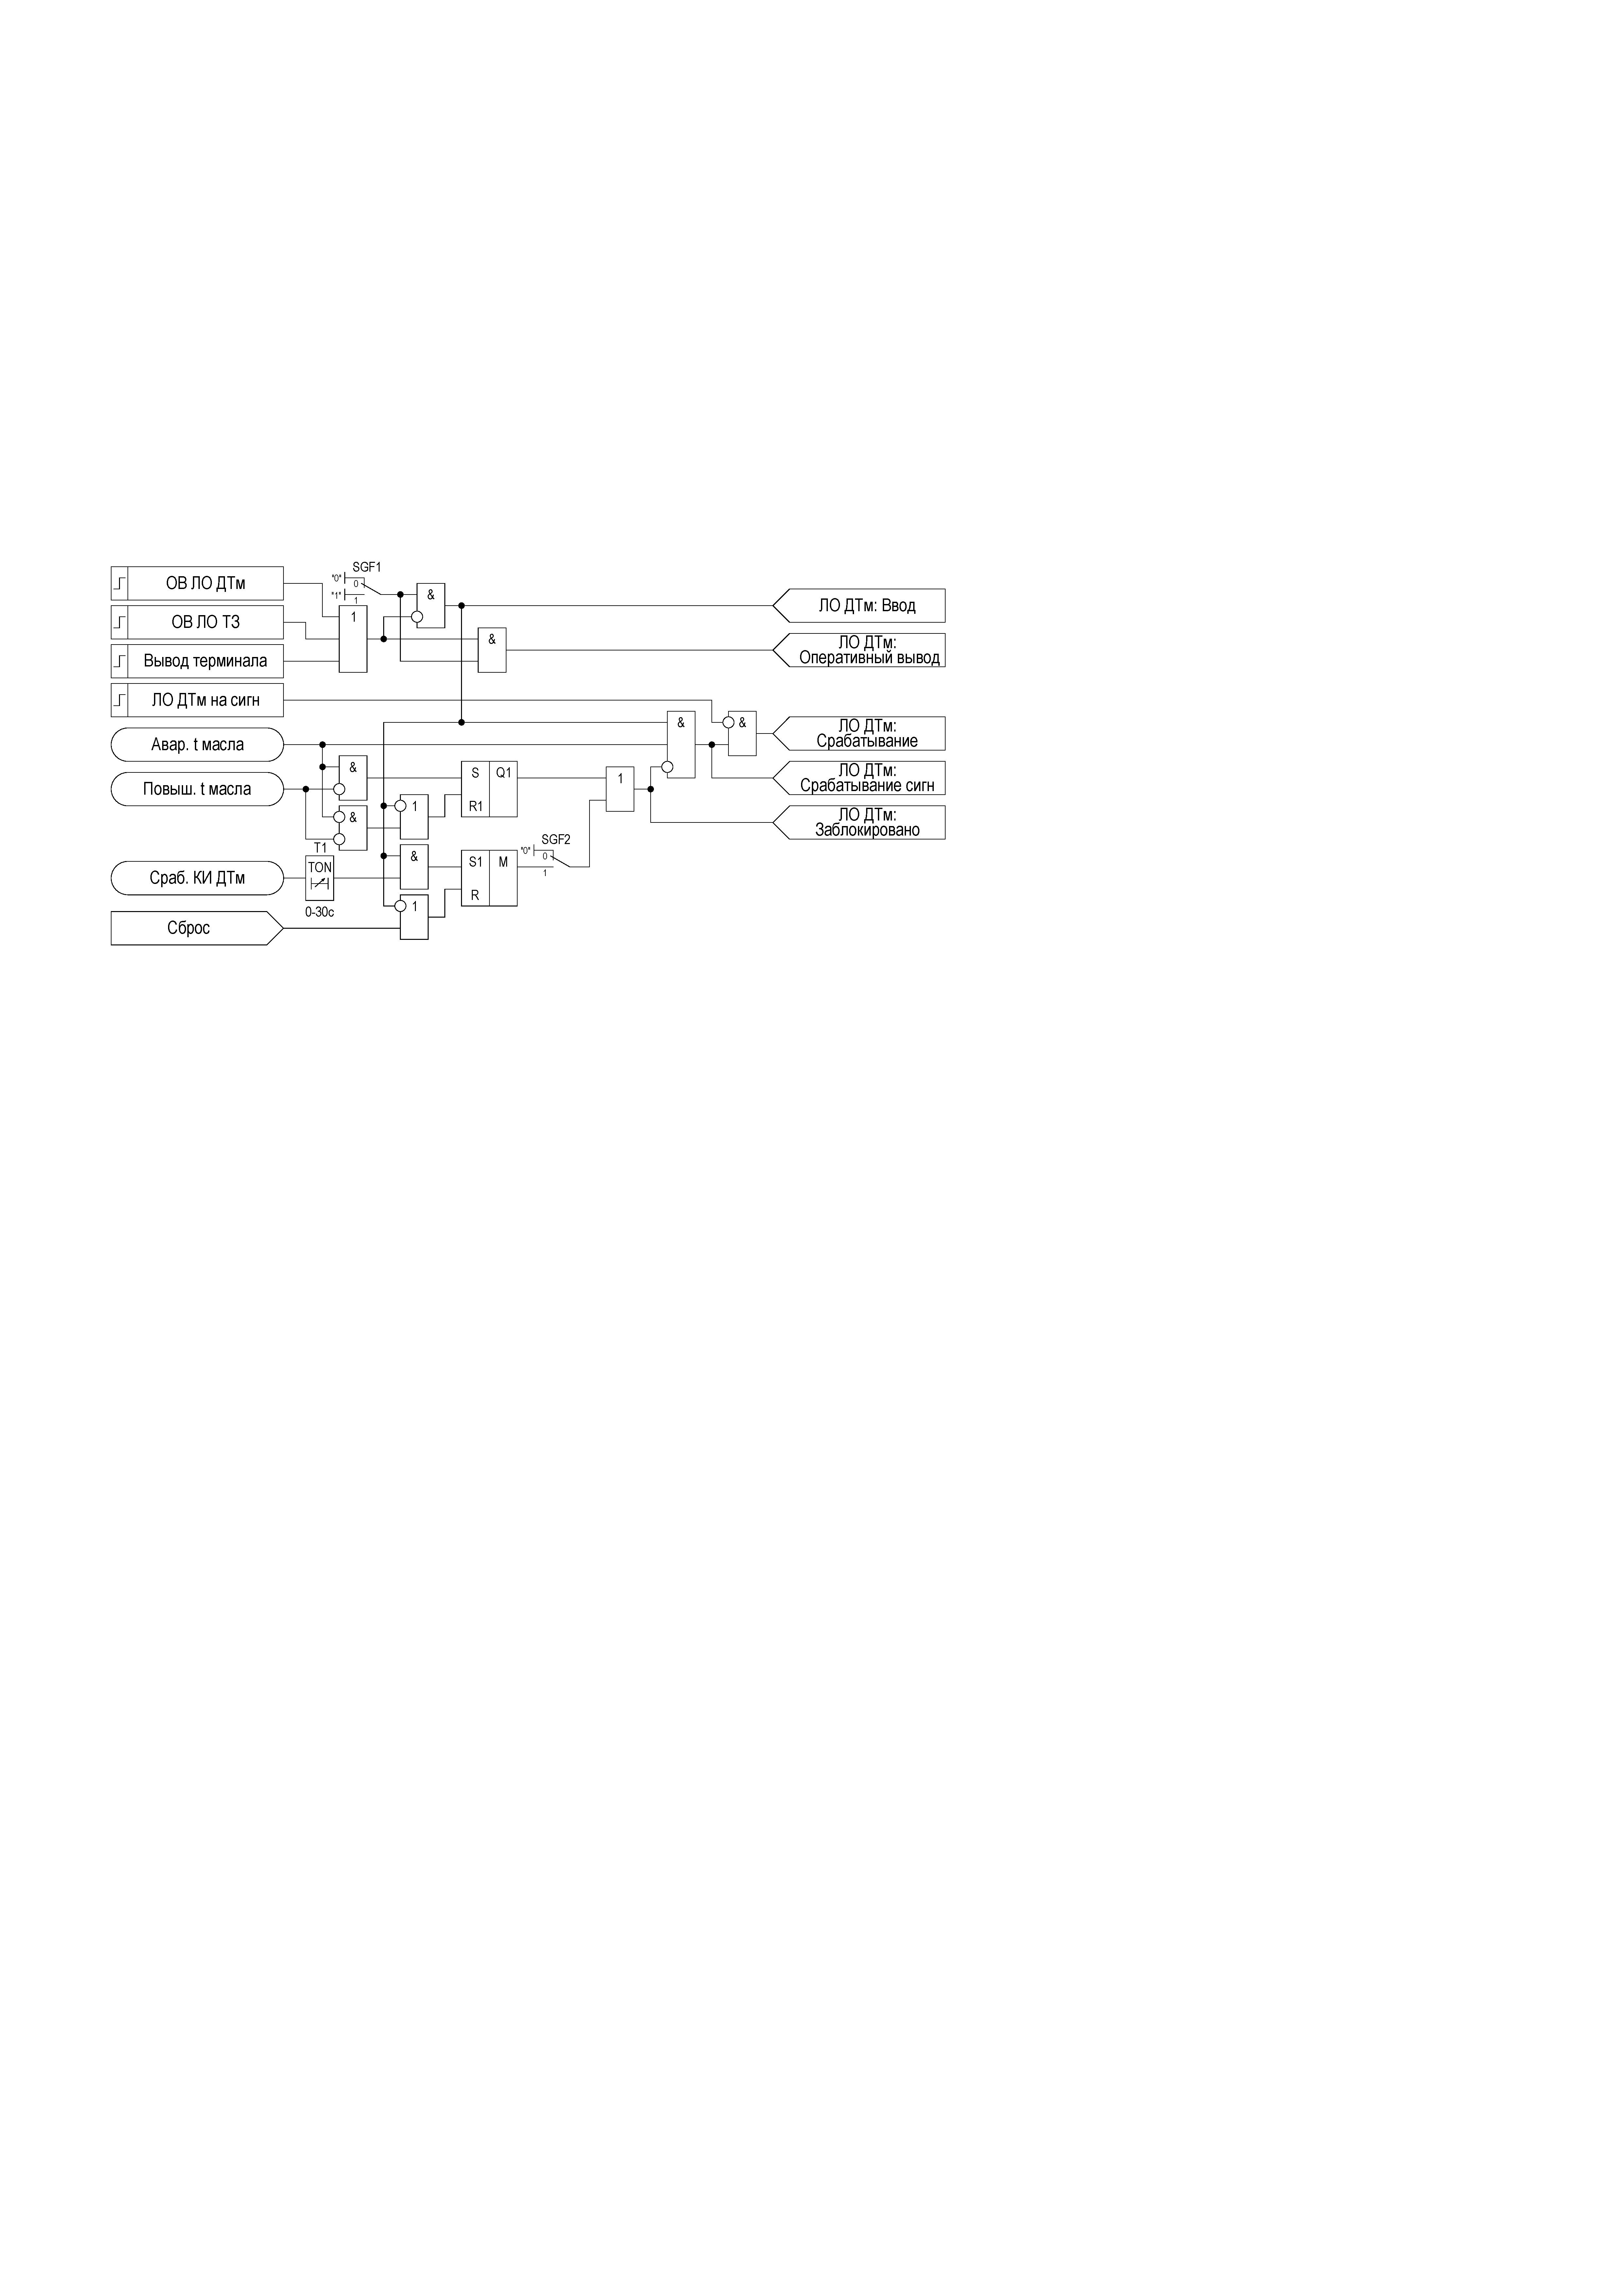
\includegraphics[width=1\textwidth,height=1\textheight,keepaspectratio]{img23.pdf}
\captionof{figure}{Функциональная схема <<ЛО~ДТм>>}
\label{lotzdtm:img1}
\end{figure}

\end{enumerate}
\FloatBarrier % Все float'ы ДО этой строки будут размещены здесь.

\item Логика отключения при срабатывании датчика температуры обмотки (ЛО ДТо)

\begin{enumerate}[label=\arabic{section}.\arabic{subsection}.\arabic{enumi}.\arabic*, labelsep=4pt, leftmargin=0em, itemindent=65pt, parsep=0pt] 

\item
Логика отключения при срабатывании датчика температуры обмотки (<<ЛО ДТо>>) служит для реализации действия на отключение трансформатора при достижении аварийного значения температуры обмотки трансформатора.

\item
Ввод функции в работу на этапе параметрирования устройства осуществляется программным переключателем SGF1 <<Ввод\_функции>>.Информация о введенной функции отображается выходным сигналом <<ЛО ДТо: Ввод>>. 
\item
Функция <<ЛО ДТо>> может быть выведена из работы оперативно путем активации сигнала <<ОВ ЛО ДТо>>, что характеризуется активным состоянием сигнала <<ЛО ДТо: Оперативный вывод>> на выходе функции. 
\item
При активном состоянии входного сигнала <<ДТо~на~сигн>> действие отключающей логики переводится на сигнал.
\item
Для формирования сигнала на отключение от <<ЛО ДТо>> при срабатывании контакта датчика температуры обмотки аварийной ступени (активное состояние входного сигнала <<Авар. t обмотки>>) необходимо также наличие сигнала срабатывания контакта датчика температуры обмотки предупредительной ступени (активное состояние входного сигнала <<Повыш. t обмотки>>), что является дополнительным подтверждающим фактором исправности цепей датчика температуры обмотки.

\item
В алгоритме предусмотрена возможность блокировки срабатывания на отключение при приеме сигнала <<Сраб. КИ ДТо>> от внешнего устройства контроля изоляции цепей датчика температуры и введенном программном переключателе SGF2 <<Блок\_от\_НИ>>. Для отстройки от кратковременных неисправностей в цепях датчика температуры может быть введена дополнительная выдержка времени таймера T1 (уставка <<Тбл>>) на прохождение сигнала <<Сраб. КИ ДТо>> в логику блокировки. 
Появление сигнала <<Сраб. КИ ДТо>> фиксируется элементом памяти, сброс блокировки осуществляется от сигнала <<Сброс>>.

\item
Алгоритм работы <<ЛО ДТо>> выполнен в соответствии с рисунком \ref{lotzdto:img1}. В таблице \ref{lotzdto:tbl1} приведены параметры, необходимые для настройки функции <<ЛО~ДТo>>.

\vspace{3mm}
\begin{figure}[H]
\centering 
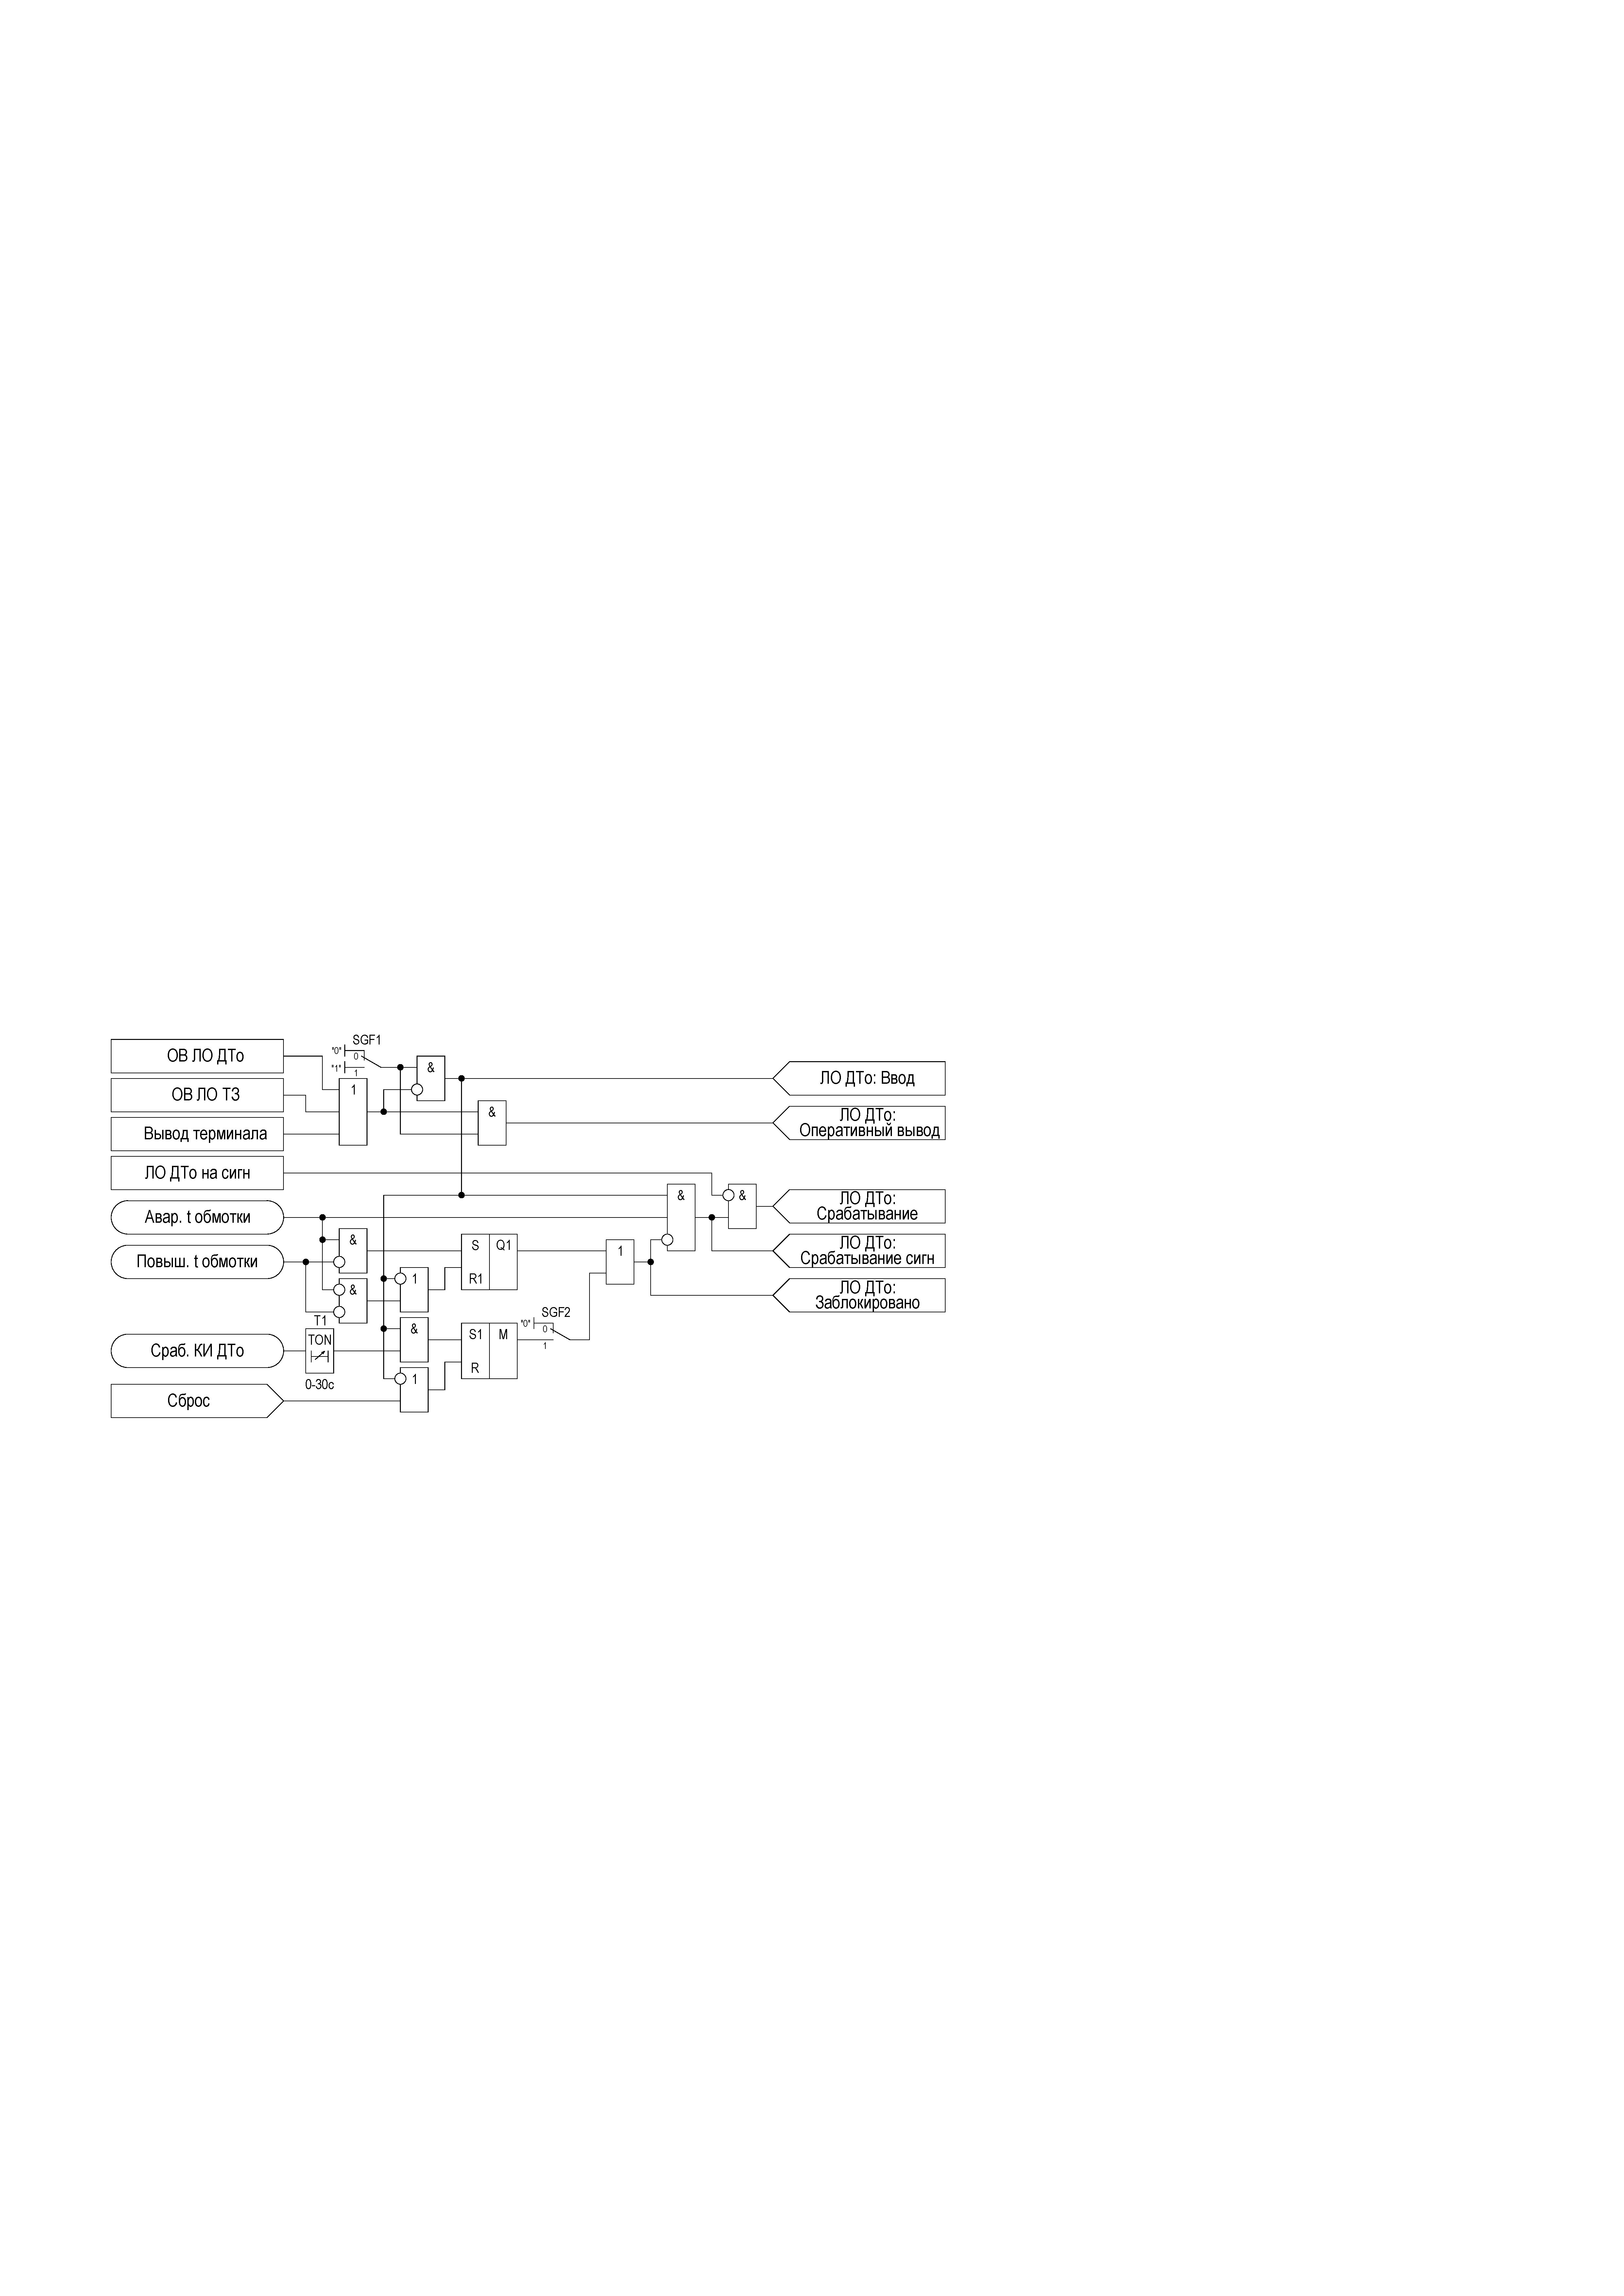
\includegraphics[width=1\textwidth,height=1\textheight,keepaspectratio]{img24.pdf}
\captionof{figure}{Функциональная схема <<ЛО ДТо>>}
\label{lotzdto:img1}
\end{figure}

\small
\begin{longtable}{|>{\centering\arraybackslash}m{5.3cm}|>{\centering\arraybackslash}m{3.3cm}|>{\centering\arraybackslash}m{4.2cm}|>{\centering\arraybackslash}m{1.8cm}|>{\centering\arraybackslash}m{1cm}|}
\caption{Параметры для настройки функции <<ЛО ДТo>>\hfill\vspace{-0.5\baselineskip}}\label{lotzdto:tbl1}\\ 
\hline
\rowcolor{gray!30}
Параметр (Параметр на ИЧМ) & Условное обозначение на схеме & Значение/ Диапазон & Единица измерения & Шаг \\ 
\hline
\endfirsthead
\caption*{\hspace{3pt}\emph{Продолжение таблицы \ref{lotzdto:tbl1}\hfill\vspace{-0.5\baselineskip}}} \\ % сделано по ГОСТ 2.105 п.6.8.7
\hline
\rowcolor{gray!30}
Параметр (Параметр на ИЧМ) & Условное обозначение на схеме & Значение/ Диапазон & Единица измерения & Шаг \\ 
\endhead
\endfoot
\endlastfoot
\centering Ввод функции в работу (Ввод\_функции) & \centering SGF1 & \centering 0 = Не предусмотрено\\1 = Предусмотрено & \centering -- & \centering \arraybackslash -- \\
\hline
\centering Блокировка от низкой изоляции (Блок\_от\_НИ) & \centering SGF2 & \centering 0 = Не предусмотрено\\1 = Предусмотрено & \centering -- & \centering \arraybackslash -- \\
\hline
\end{longtable}
\normalsize

\end{enumerate}
\FloatBarrier % Все float'ы ДО этой строки будут размещены здесь.

\item Логика отключения при срабатывании реле давления трансформатора (ЛО РД)

\begin{enumerate}[label=\arabic{section}.\arabic{subsection}.\arabic{enumi}.\arabic*, labelsep=4pt, leftmargin=0em, itemindent=65pt, parsep=0pt] 

\item
Логика отключения при срабатывании реле давления трансформатора (<<ЛО РД>>) служит для реализации действия на отключение трансформатора при срабатывании реле давления трансформатора.
\item
Ввод функции в работу на этапе параметрирования устройства осуществляется программным переключателем SGF1 <<Ввод\_функции>>. Информация о введенной функции отображается выходным сигналом <<ЛО РД: Ввод>>.
\item
Функция <<ЛО РД>> может быть выведена из работы оперативно путем активации сигнала <<ОВ ЛО РД>>, что характеризуется активным состоянием сигнала <<ЛО РД: Оперативный вывод>> на выходе функции.
\item
При активном состоянии входного сигнала <<РД~на~сигн>> действие отключающей логики переводится на сигнал.
\item
В алгоритме предусмотрена возможность блокировки срабатывания на отключение при приеме сигнала <<Сраб. КИ датч.давл.>> от внешнего устройства контроля изоляции цепей реле давления и введенном программном переключателе SGF2 <<Блок\_от\_НИ>>. Для отстройки от кратковременных неисправностей в цепях реле давления может быть введена дополнительная выдержка времени таймера T1 (уставка <<Тбл>>) на прохождение сигнала <<Сраб. КИ датч.давл.>> в логику блокировки. 
Появление сигнала <<Сраб. КИ датч.давл.>> фиксируется элементом памяти, сброс блокировки осуществляется от сигнала <<Сброс>>.

\item
Алгоритм работы <<ЛО РД>> выполнен в соответствии с рисунком \ref{lotzrd:img1}. В таблице \ref{lotzrd:tbl1} приведены параметры, необходимые для настройки функции <<ЛО РД>>.

\vspace{3mm}
\begin{figure}[H]
\centering
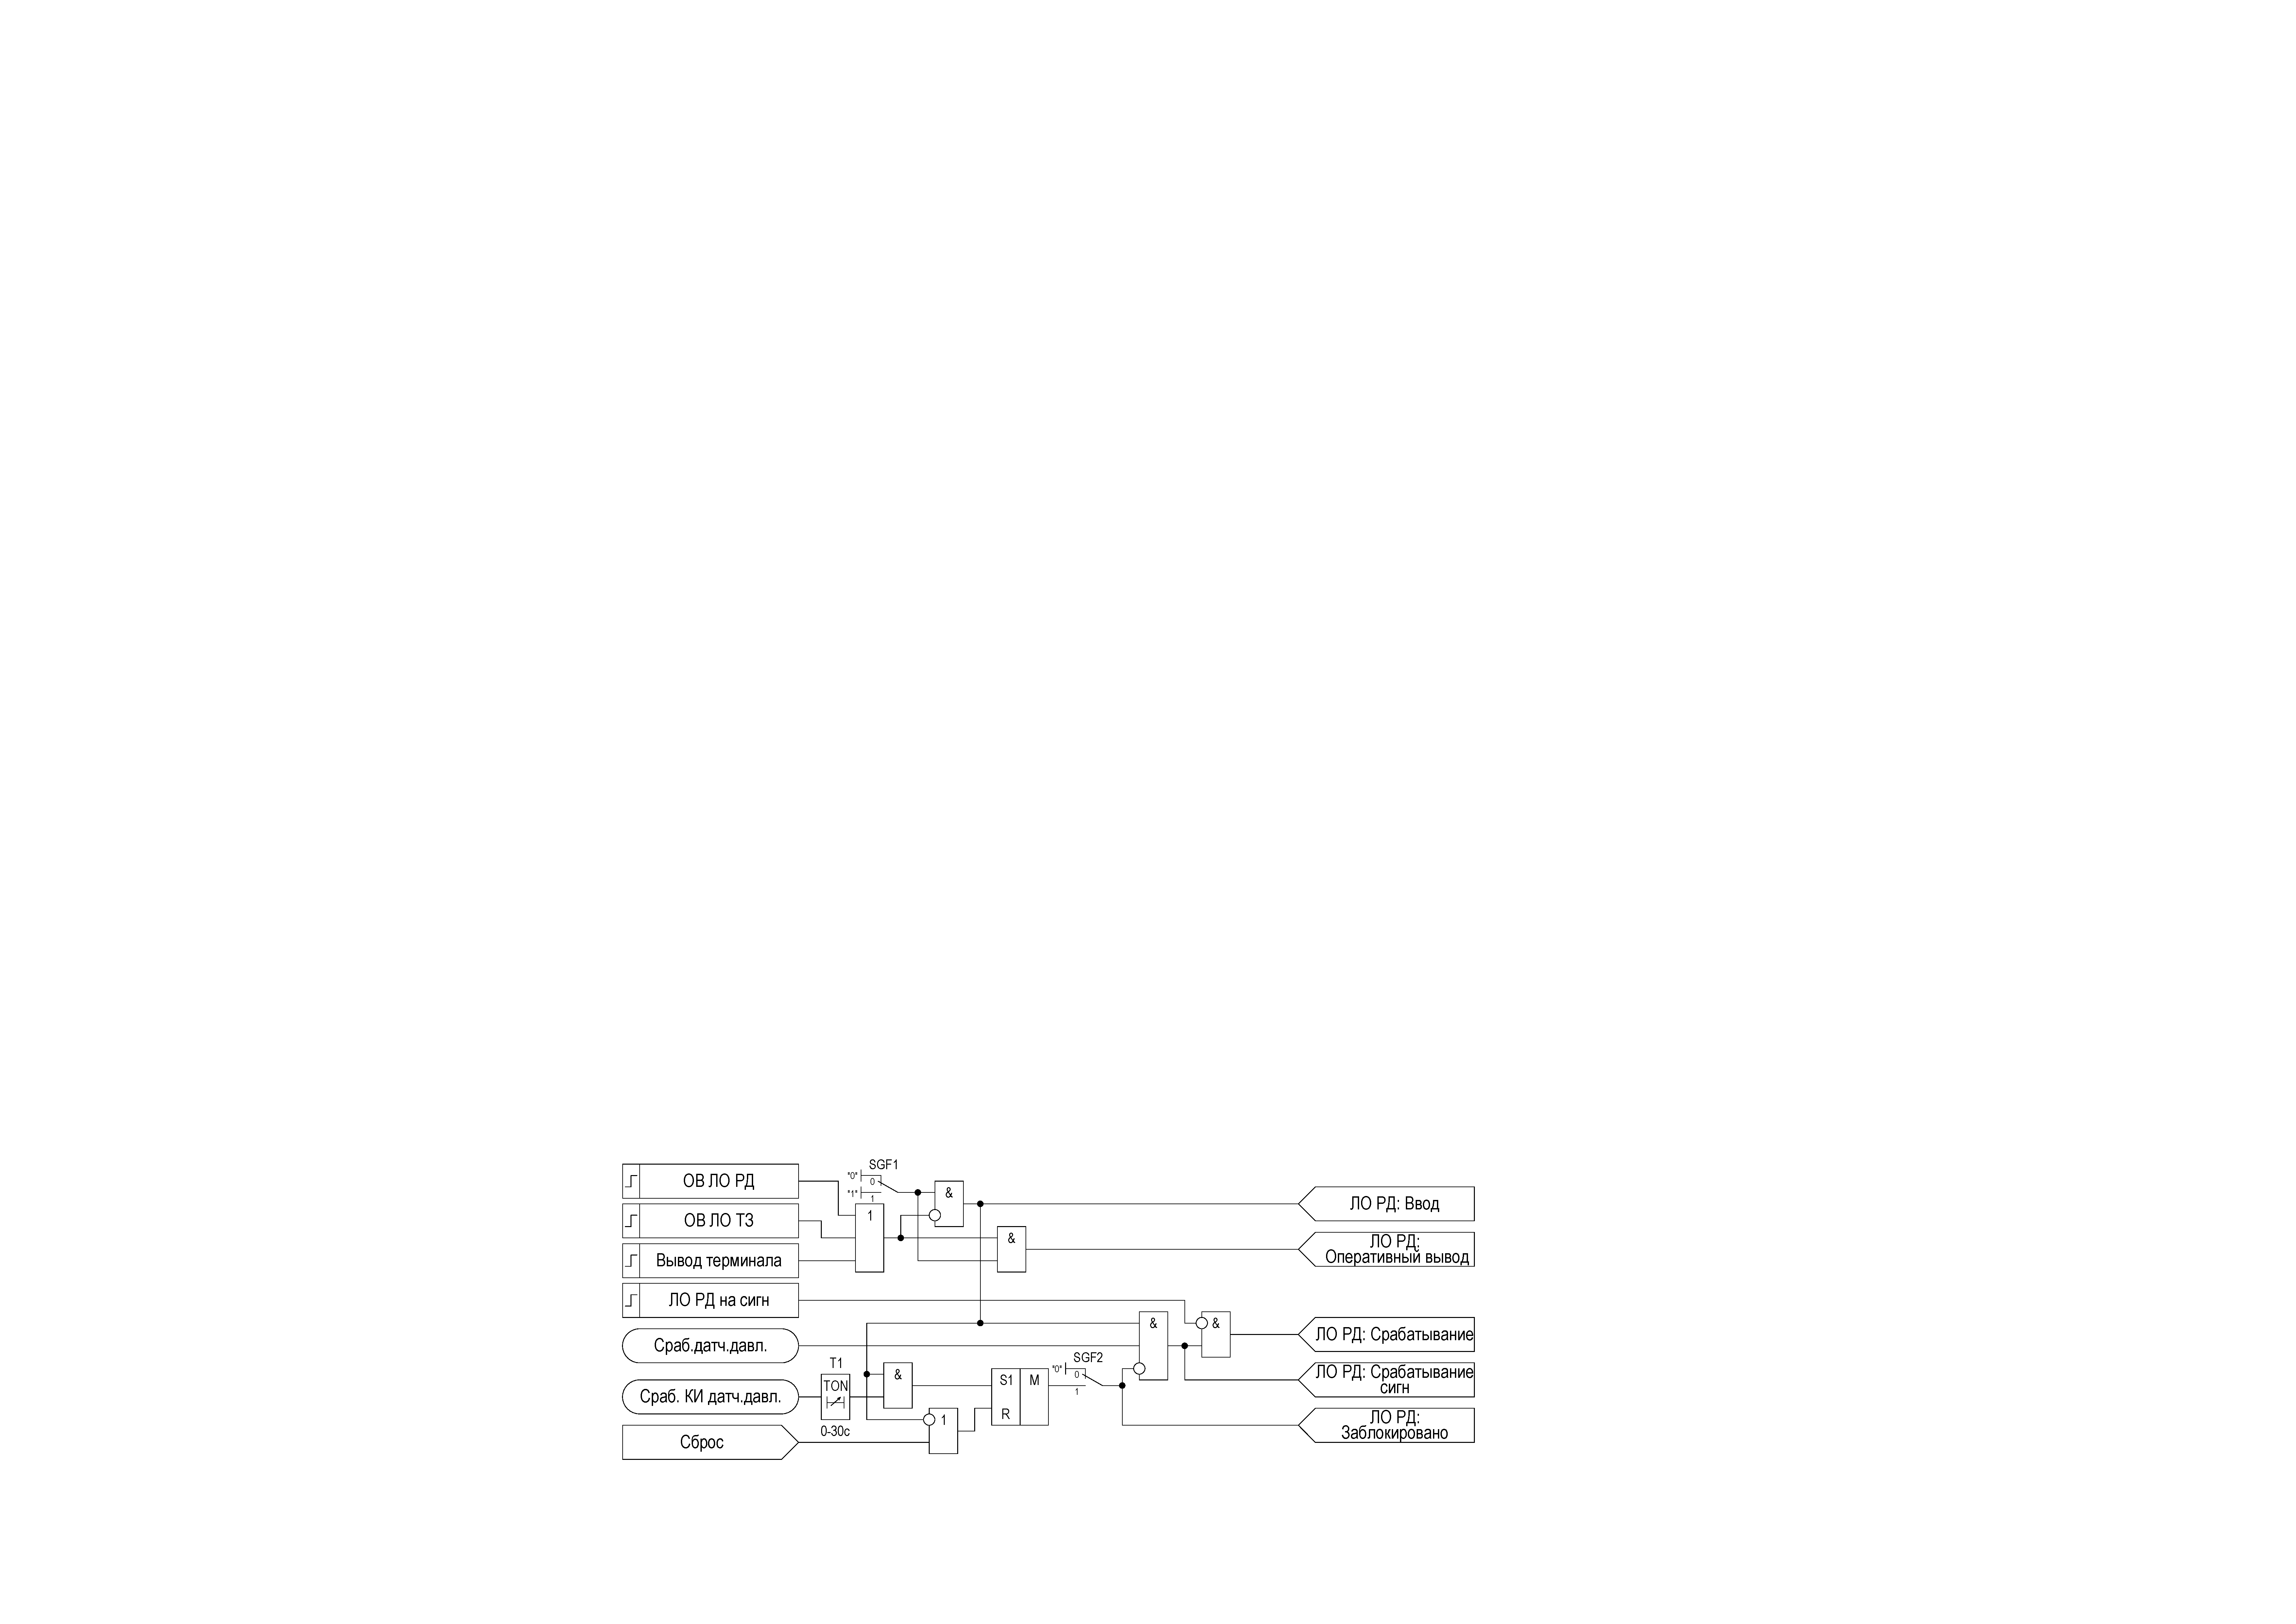
\includegraphics[width=1\textwidth,height=1\textheight,keepaspectratio]{img25.pdf}
\captionof{figure}{Функциональная схема <<ЛО РД>>}
\label{lotzrd:img1}
\end{figure}

\small
\begin{longtable}{|>{\centering\arraybackslash}m{5.3cm}|>{\centering\arraybackslash}m{3.3cm}|>{\centering\arraybackslash}m{4.2cm}|>{\centering\arraybackslash}m{1.8cm}|>{\centering\arraybackslash}m{1cm}|}
\caption{Параметры для настройки функции <<ЛО РД>>\hfill\vspace{-0.5\baselineskip}}\label{lotzrd:tbl1}\\ 
\hline
\rowcolor{gray!30}
Параметр (Параметр на ИЧМ) & Условное обозначение на схеме & Значение/ Диапазон & Единица измерения & Шаг \\ 
\hline
\endfirsthead
\caption*{\hspace{3pt}\emph{Продолжение таблицы \ref{lotzrd:tbl1}\hfill\vspace{-0.5\baselineskip}}} \\ % сделано по ГОСТ 2.105 п.6.8.7
\hline
\rowcolor{gray!30}
Параметр (Параметр на ИЧМ) & Условное обозначение на схеме & Значение/ Диапазон & Единица измерения & Шаг \\ 
\endhead
\endfoot
\endlastfoot
\centering Ввод функции в работу (Ввод\_функции) & \centering SGF1 & \centering 0 = Не предусмотрено\\1 = Предусмотрено & \centering -- & \centering \arraybackslash -- \\
\hline
\centering Блокировка от низкой изоляции (Блок\_от\_НИ) & \centering SGF2 & \centering 0 = Не предусмотрено\\1 = Предусмотрено & \centering -- & \centering \arraybackslash -- \\
\hline
\end{longtable}
\normalsize

\end{enumerate}

\end{enumerate}
\FloatBarrier % Все float'ы ДО этой строки будут размещены здесь.
\needspace{4\baselineskip}
\color{uniblue}{\subsection{\sloppy Логика отключения при срабатывании технологической сигнализации \mbox{трансформатора} (ЛО~ТС)}}
\color{black}

\begin{enumerate}[label=\arabic{section}.\arabic{subsection}.\arabic{enumi}, labelsep=4pt, leftmargin=0pt, itemindent=57pt, itemsep=0pt, parsep=5pt] % если что можно крутить itemsep

\item Общие сведения

\begin{enumerate}[label=\arabic{section}.\arabic{subsection}.\arabic{enumi}.\arabic*, labelsep=4pt, leftmargin=0em, itemindent=65pt, parsep=0pt]

\item
Логика отключения при срабатывании технологической сигнализации служит для реализации действия на отключение трансформатора при срабатывании датчиков технологической сигнализации трансформатора в случае необходимости или требований.
\item
Функциональный блок <<ЛО~ТС>> может быть выведен из работы оперативно путем активации сигнала <<ОВ~ЛО~ТС>>.
\item
В функциональном блоке реализована возможность приема следующих сигналов датчиков технологической сигнализации трансформатора:
\begin{itemize}
\item открытое состояние предохранительного клапана для функции <<ЛО ПК>>;
\item закрытое состояние отсечного клапана для функции <<ЛО ОК>>;
\item низкий уровень масла в расширительном баке трансформатора для функции <<ЛО ДУм расширителя>>.
\end{itemize}
\item
Функциональный блок <<ЛО~ТС>> используется в случае необходимости действия на отключение трансформатора при срабатывании датчиков технологической сигнализации.

\end{enumerate}

\item Логика отключения при срабатывании предохранительного клапана (ЛО~ПК)

\begin{enumerate}[label=\arabic{section}.\arabic{subsection}.\arabic{enumi}.\arabic*, labelsep=4pt, leftmargin=0em, itemindent=65pt, parsep=0pt]

\item
Логика отключения при срабатывании предохранительного клапана (<<ЛО ПК>>) служит для реализации действия на отключение трансформатора при срабатывании предохранительного клапана трансформатора.
\item
Ввод функции в работу на этапе параметрирования устройства осуществляется программным переключателем SGF1 <<Ввод\_функции>>. Информация о введенной функции отображается выходным сигналом <<ЛО ПК: Ввод>>.
\item
Функция <<ЛО ПК>> может быть выведена из работы оперативно путем активации сигнала <<ОВ ЛО ПК>>, что характеризуется активным состоянием сигнала <<ЛО ПК: Оперативный вывод>> на выходе функции.
\item
При активном состоянии входного сигнала <<ПК~на~сигн>> действие отключающей логики переводится на сигнал.
\item
Алгоритм работы <<ЛО ПК>> выполнен в соответствии с рисунком \ref{lotspk:img1}. В таблице \ref{lotspk:tbl1} приведены параметры, необходимые для настройки функции <<ЛО ПК>>.

\small
\begin{longtable}{|>{\centering\arraybackslash}m{5.3cm}|>{\centering\arraybackslash}m{3.3cm}|>{\centering\arraybackslash}m{4.2cm}|>{\centering\arraybackslash}m{1.8cm}|>{\centering\arraybackslash}m{1cm}|}
\caption{Параметры для настройки функции <<ЛО ПК>>\hfill\vspace{-0.5\baselineskip}}\label{lotspk:tbl1}\\ 
\hline
\rowcolor{gray!30}
Параметр (Параметр на ИЧМ) & Условное обозначение на схеме & Значение/ Диапазон & Единица измерения & Шаг \\ 
\hline
\endfirsthead
\caption*{\hspace{3pt}\emph{Продолжение таблицы \ref{lotspk:tbl1}\hfill\vspace{-0.5\baselineskip}}} \\ % сделано по ГОСТ 2.105 п.6.8.7
\hline
\rowcolor{gray!30}
Параметр (Параметр на ИЧМ) & Условное обозначение на схеме & Значение/ Диапазон & Единица измерения & Шаг \\ 
\endhead
\endfoot
\endlastfoot
\centering Ввод функции в работу (Ввод\_функции) & \centering SGF1 & \centering 0 = Не предусмотрено\\1 = Предусмотрено & \centering -- & \centering \arraybackslash -- \\
\hline
\end{longtable}
\normalsize

\vspace{3mm}
\begin{figure}[H]
\centering
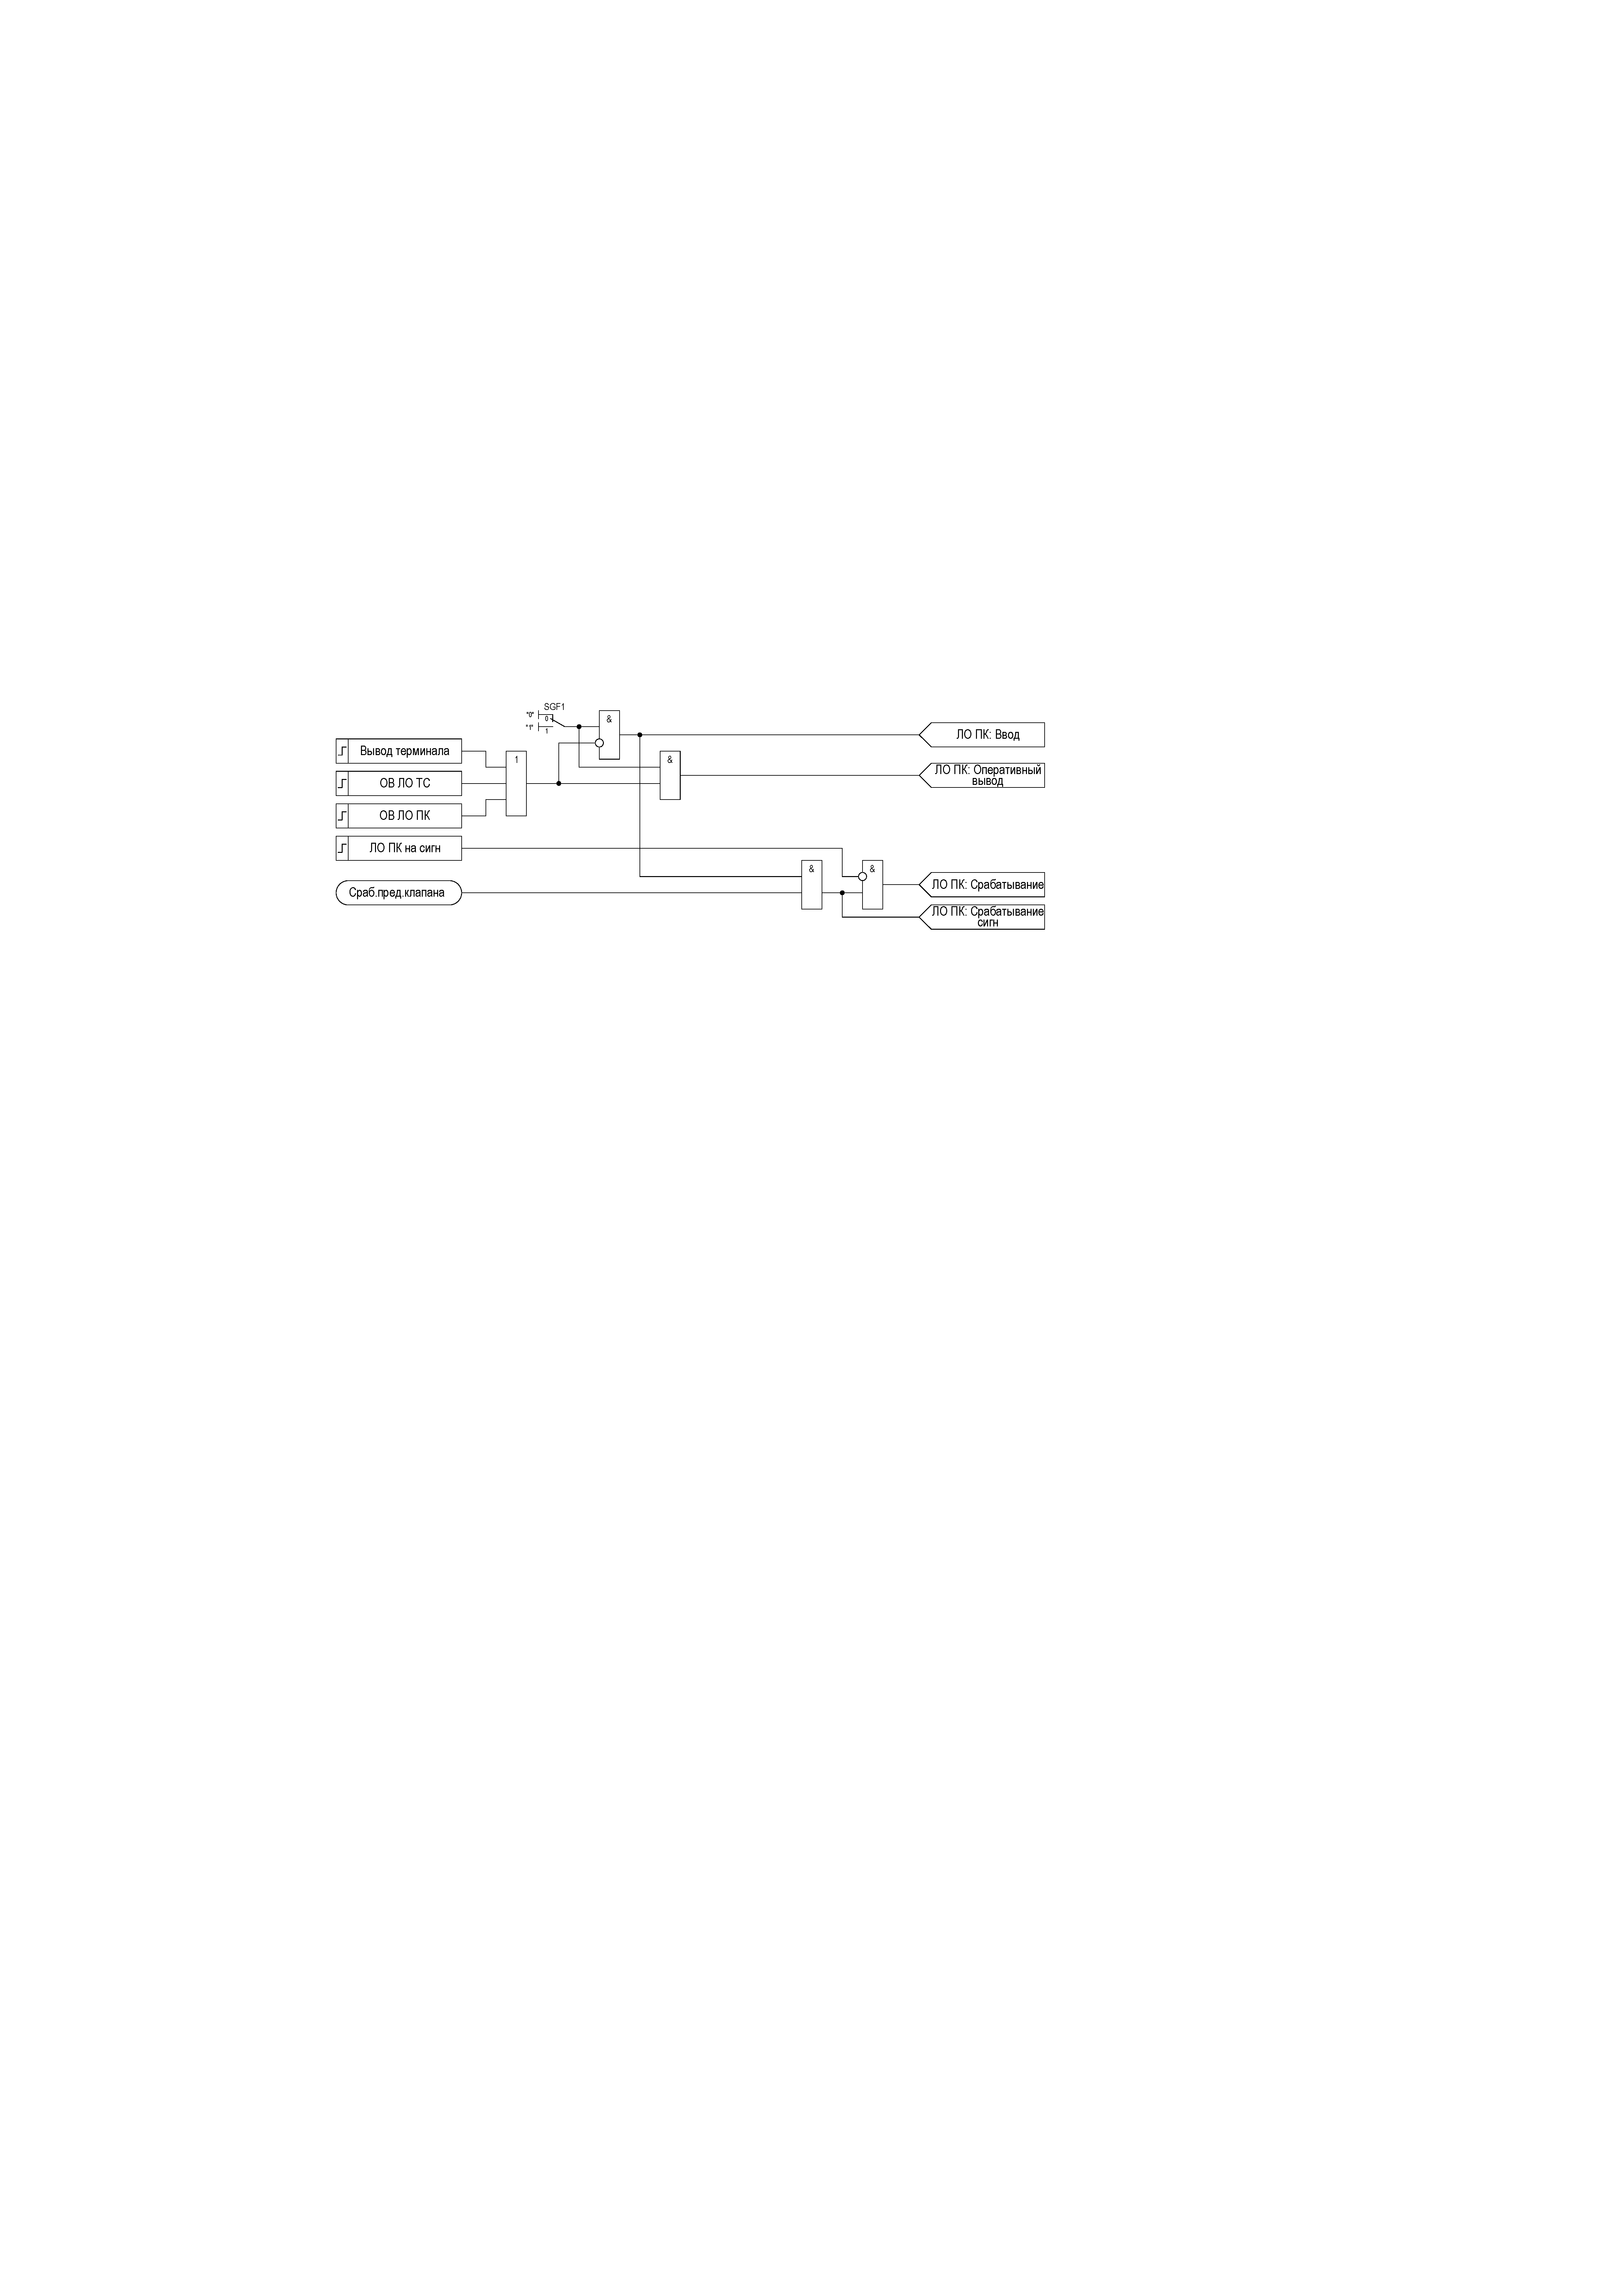
\includegraphics[width=1\textwidth,height=1\textheight,keepaspectratio]{img26.pdf}
\captionof{figure}{Функциональная схема <<ЛО ПК>>}
\label{lotspk:img1}
\end{figure}

\end{enumerate}
\FloatBarrier % Все float'ы ДО этой строки будут размещены здесь.
\item Логика отключения при срабатывании отсечного клапана (ЛО~ОК)

\begin{enumerate}[label=\arabic{section}.\arabic{subsection}.\arabic{enumi}.\arabic*, labelsep=4pt, leftmargin=0em, itemindent=65pt, parsep=0pt]

\item
Логика отключения при срабатывании отсечного клапана (<<ЛО~ОК>>) служит для реализации действия на отключение трансформатора при срабатывании отсечного клапана трансформатора.
\item
Ввод функции в работу на этапе параметрирования устройства осуществляется программным переключателем SGF1 <<Ввод\_функции>>. Информация о введенной функции отображается выходным сигналом <<ЛО ОК: Ввод>>.
\item
Функция <<ЛО ПК>> может быть выведена из работы оперативно путем активации сигнала <<ОВ ЛО ОК>>, что характеризуется активным состоянием сигнала <<ЛО ОК: Оперативный вывод>> на выходе функции. 
\item
При активном состоянии входного сигнала <<ОК~на~сигн>> действие отключающей логики переводится на сигнал.
\item
Алгоритм работы <<ЛО ОК>> выполнен в соответствии с рисунком \ref{lotsok:img1}. В таблице \ref{lotsok:tbl1} приведены параметры, необходимые для настройки функции <<ЛО ОК>>.

\small
\begin{longtable}{|>{\centering\arraybackslash}m{5.3cm}|>{\centering\arraybackslash}m{3.3cm}|>{\centering\arraybackslash}m{4.2cm}|>{\centering\arraybackslash}m{1.8cm}|>{\centering\arraybackslash}m{1cm}|}
\caption{Параметры для настройки функции <<ЛО ОК>>\hfill\vspace{-0.5\baselineskip}}\label{lotsok:tbl1}\\ 
\hline
\rowcolor{gray!30}
Параметр (Параметр на ИЧМ) & Условное обозначение на схеме & Значение/ Диапазон & Единица измерения & Шаг \\ 
\hline
\endfirsthead
\caption*{\hspace{3pt}\emph{Продолжение таблицы \ref{lotsok:tbl1}\hfill\vspace{-0.5\baselineskip}}} \\ % сделано по ГОСТ 2.105 п.6.8.7
\hline
\rowcolor{gray!30}
Параметр (Параметр на ИЧМ) & Условное обозначение на схеме & Значение/ Диапазон & Единица измерения & Шаг \\ 
\endhead
\endfoot
\endlastfoot
\centering Ввод функции в работу (Ввод\_функции) & \centering SGF1 & \centering 0 = Не предусмотрено\\1 = Предусмотрено & \centering -- & \centering \arraybackslash -- \\
\hline
\end{longtable}
\normalsize

\vspace{3mm}
\begin{figure}[H]
\centering
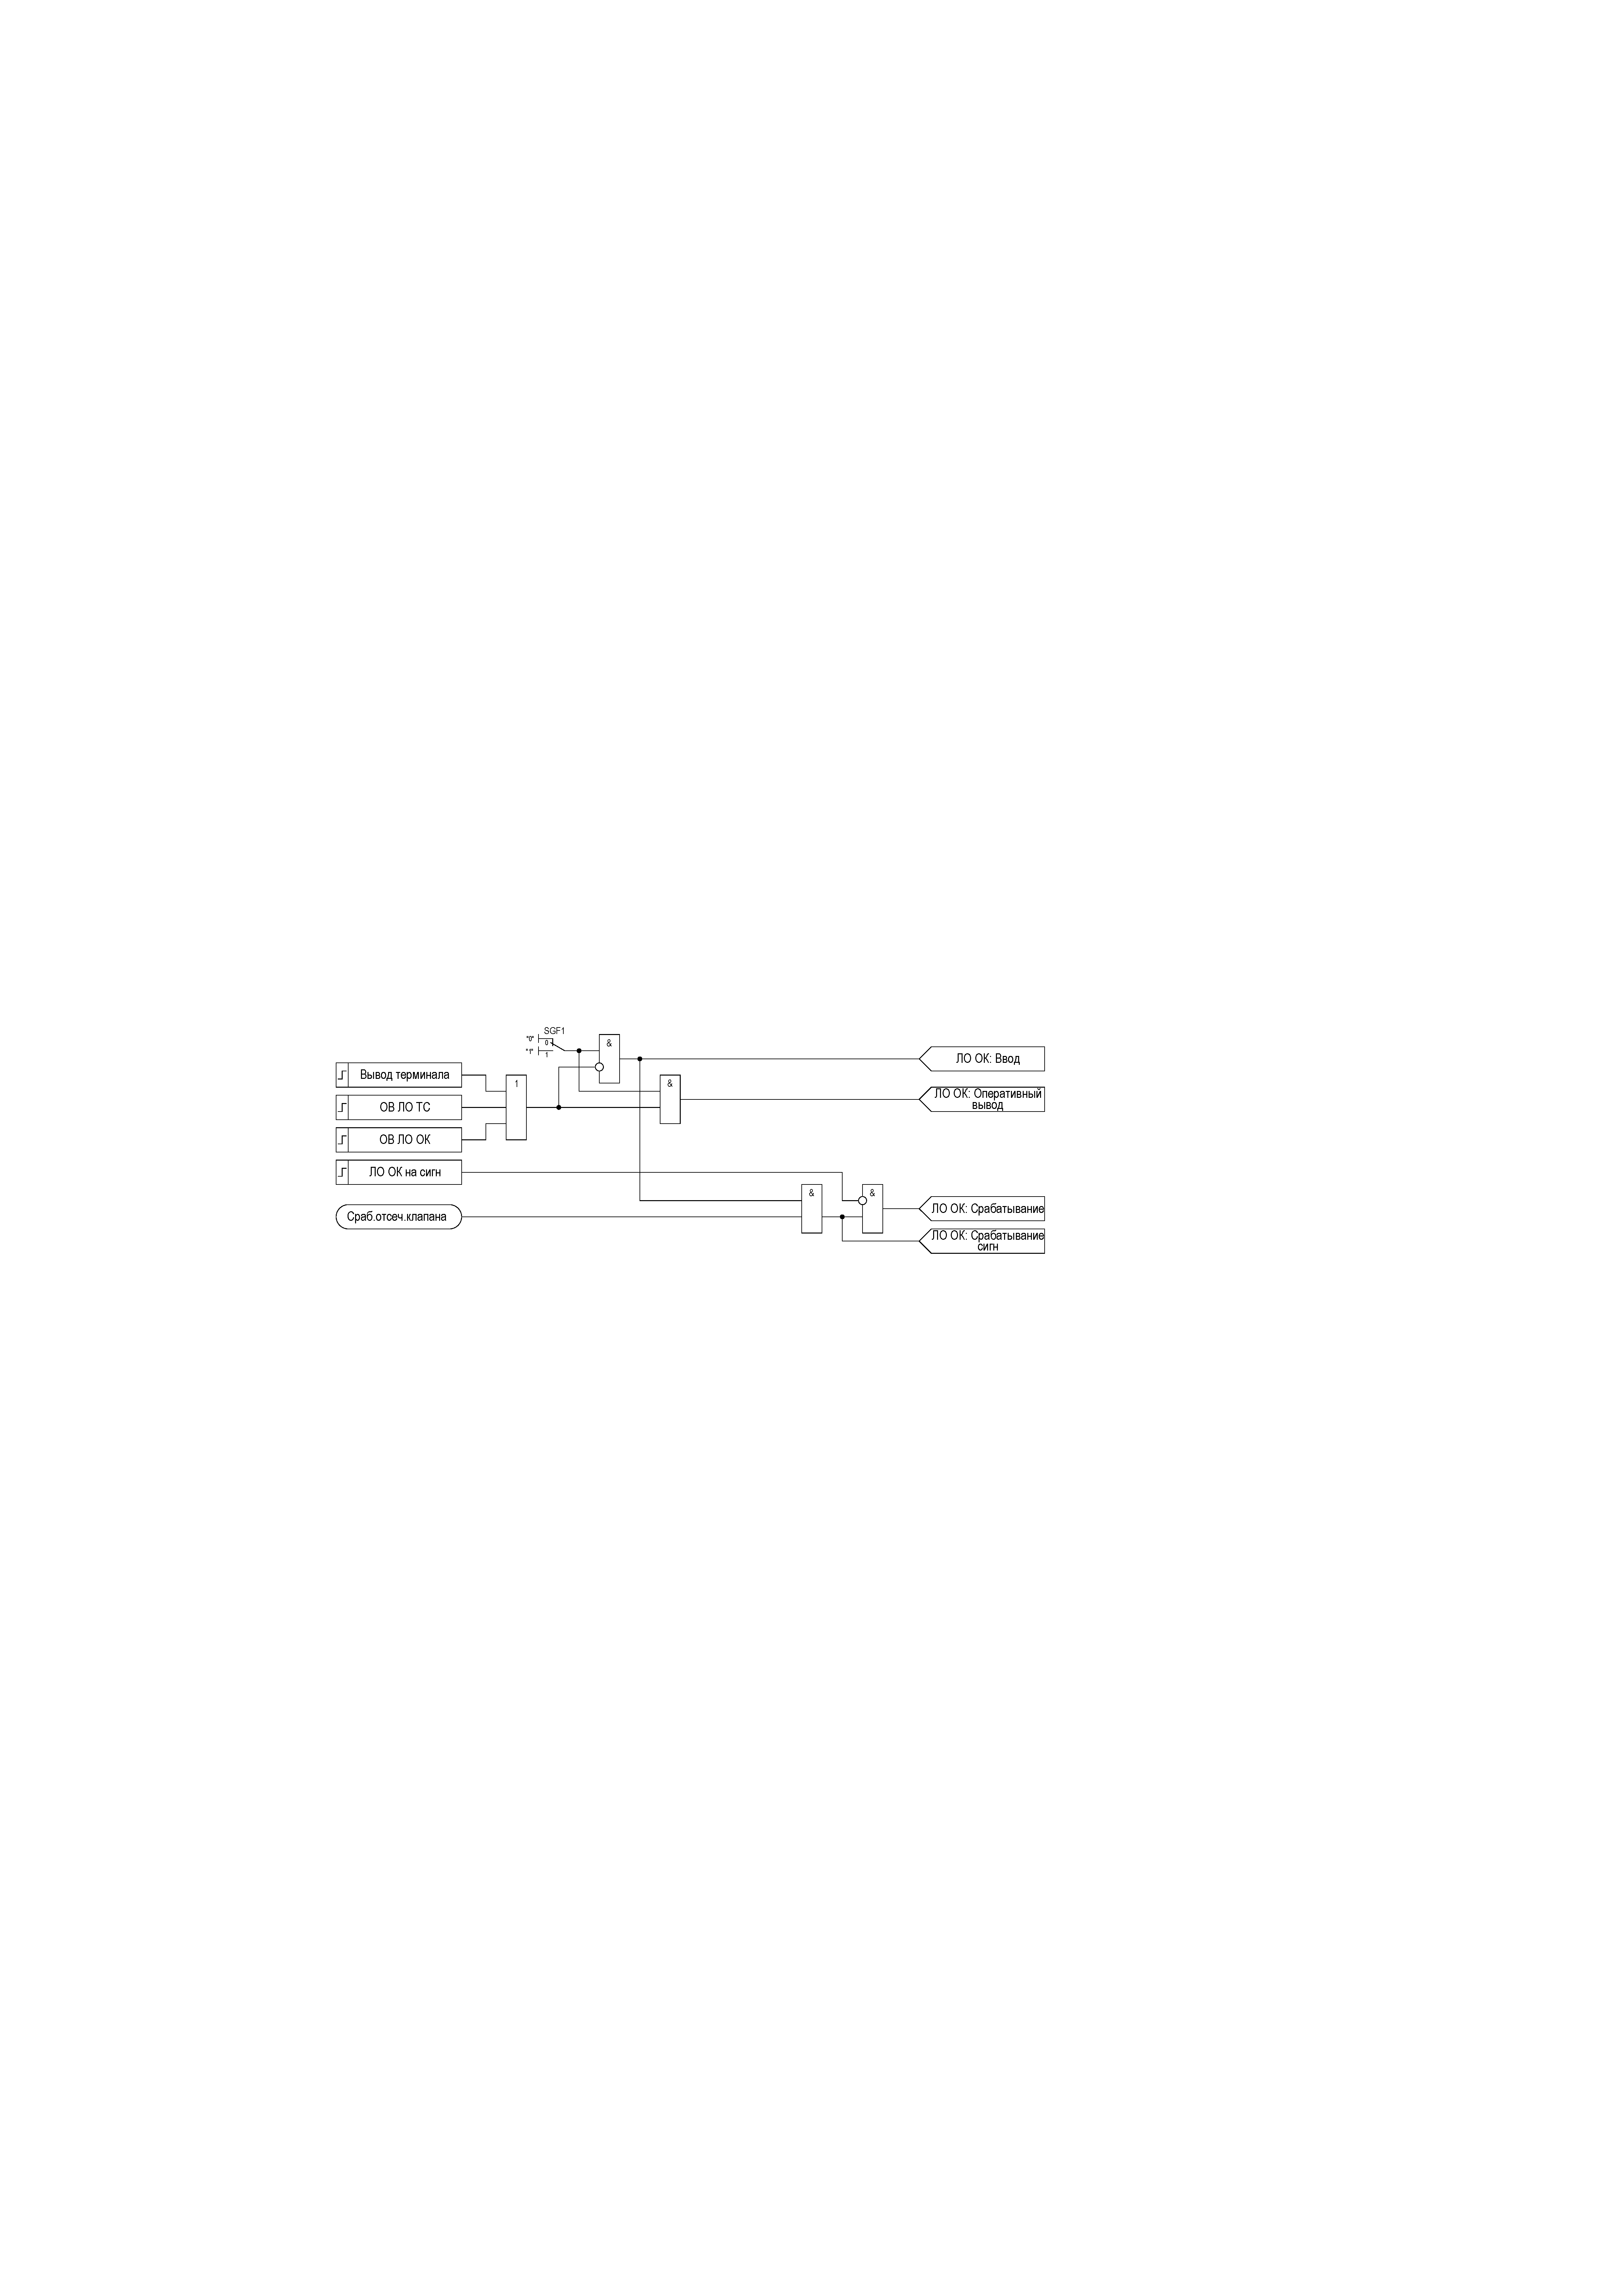
\includegraphics[width=1\textwidth,height=1\textheight,keepaspectratio]{img27.pdf}
\captionof{figure}{Функциональная схема <<ЛО~ОК>>}\label{lotsok:img1}
\end{figure}

\end{enumerate}
\FloatBarrier % Все float'ы ДО этой строки будут размещены здесь.

\item Логика отключения при снижении уровня масла в расширительном баке трансформатора (ЛО~ДУм расширителя)

\begin{enumerate}[label=\arabic{section}.\arabic{subsection}.\arabic{enumi}.\arabic*, labelsep=4pt, leftmargin=0em, itemindent=65pt, parsep=0pt]

\item
Логика отключения при снижении уровня масла в расширительном баке трансформатора (<<ЛО~ДУм расширителя>>) служит для реализации действия на отключение трансформатора при снижении уровня масла в расширительном баке трансформатора.
\item
Ввод функции в работу на этапе параметрирования устройства осуществляется программным переключателем SGF1 <<Ввод\_функции>>. Информация о введенной функции отображается выходным сигналом <<ЛО~ДУм расширителя: Ввод>>.
\item
Функция <<ЛО~ДУм расширителя>> может быть выведена из работы оперативно путем активации сигнала <<ОВ ЛО ДУм расшир>>, что характеризуется активным состоянием сигнала <<ЛО~ДУм расшир: Оперативный вывод>> на выходе функции. 
\item
При активном состоянии входного сигнала <<ДУм расшир~на~сигн>> действие отключающей логики переводится на сигнал. 
\item
Алгоритм работы <<ЛО~ДУм расширителя>> выполнен в соответствии с рисунком \ref{lotsdut:img1}. В таблице \ref{lotsdut:tbl1} приведены параметры, необходимые для настройки функции <<ЛО~ДУм расширителя>>.

\vspace{3mm}
\begin{figure}[H]
\centering
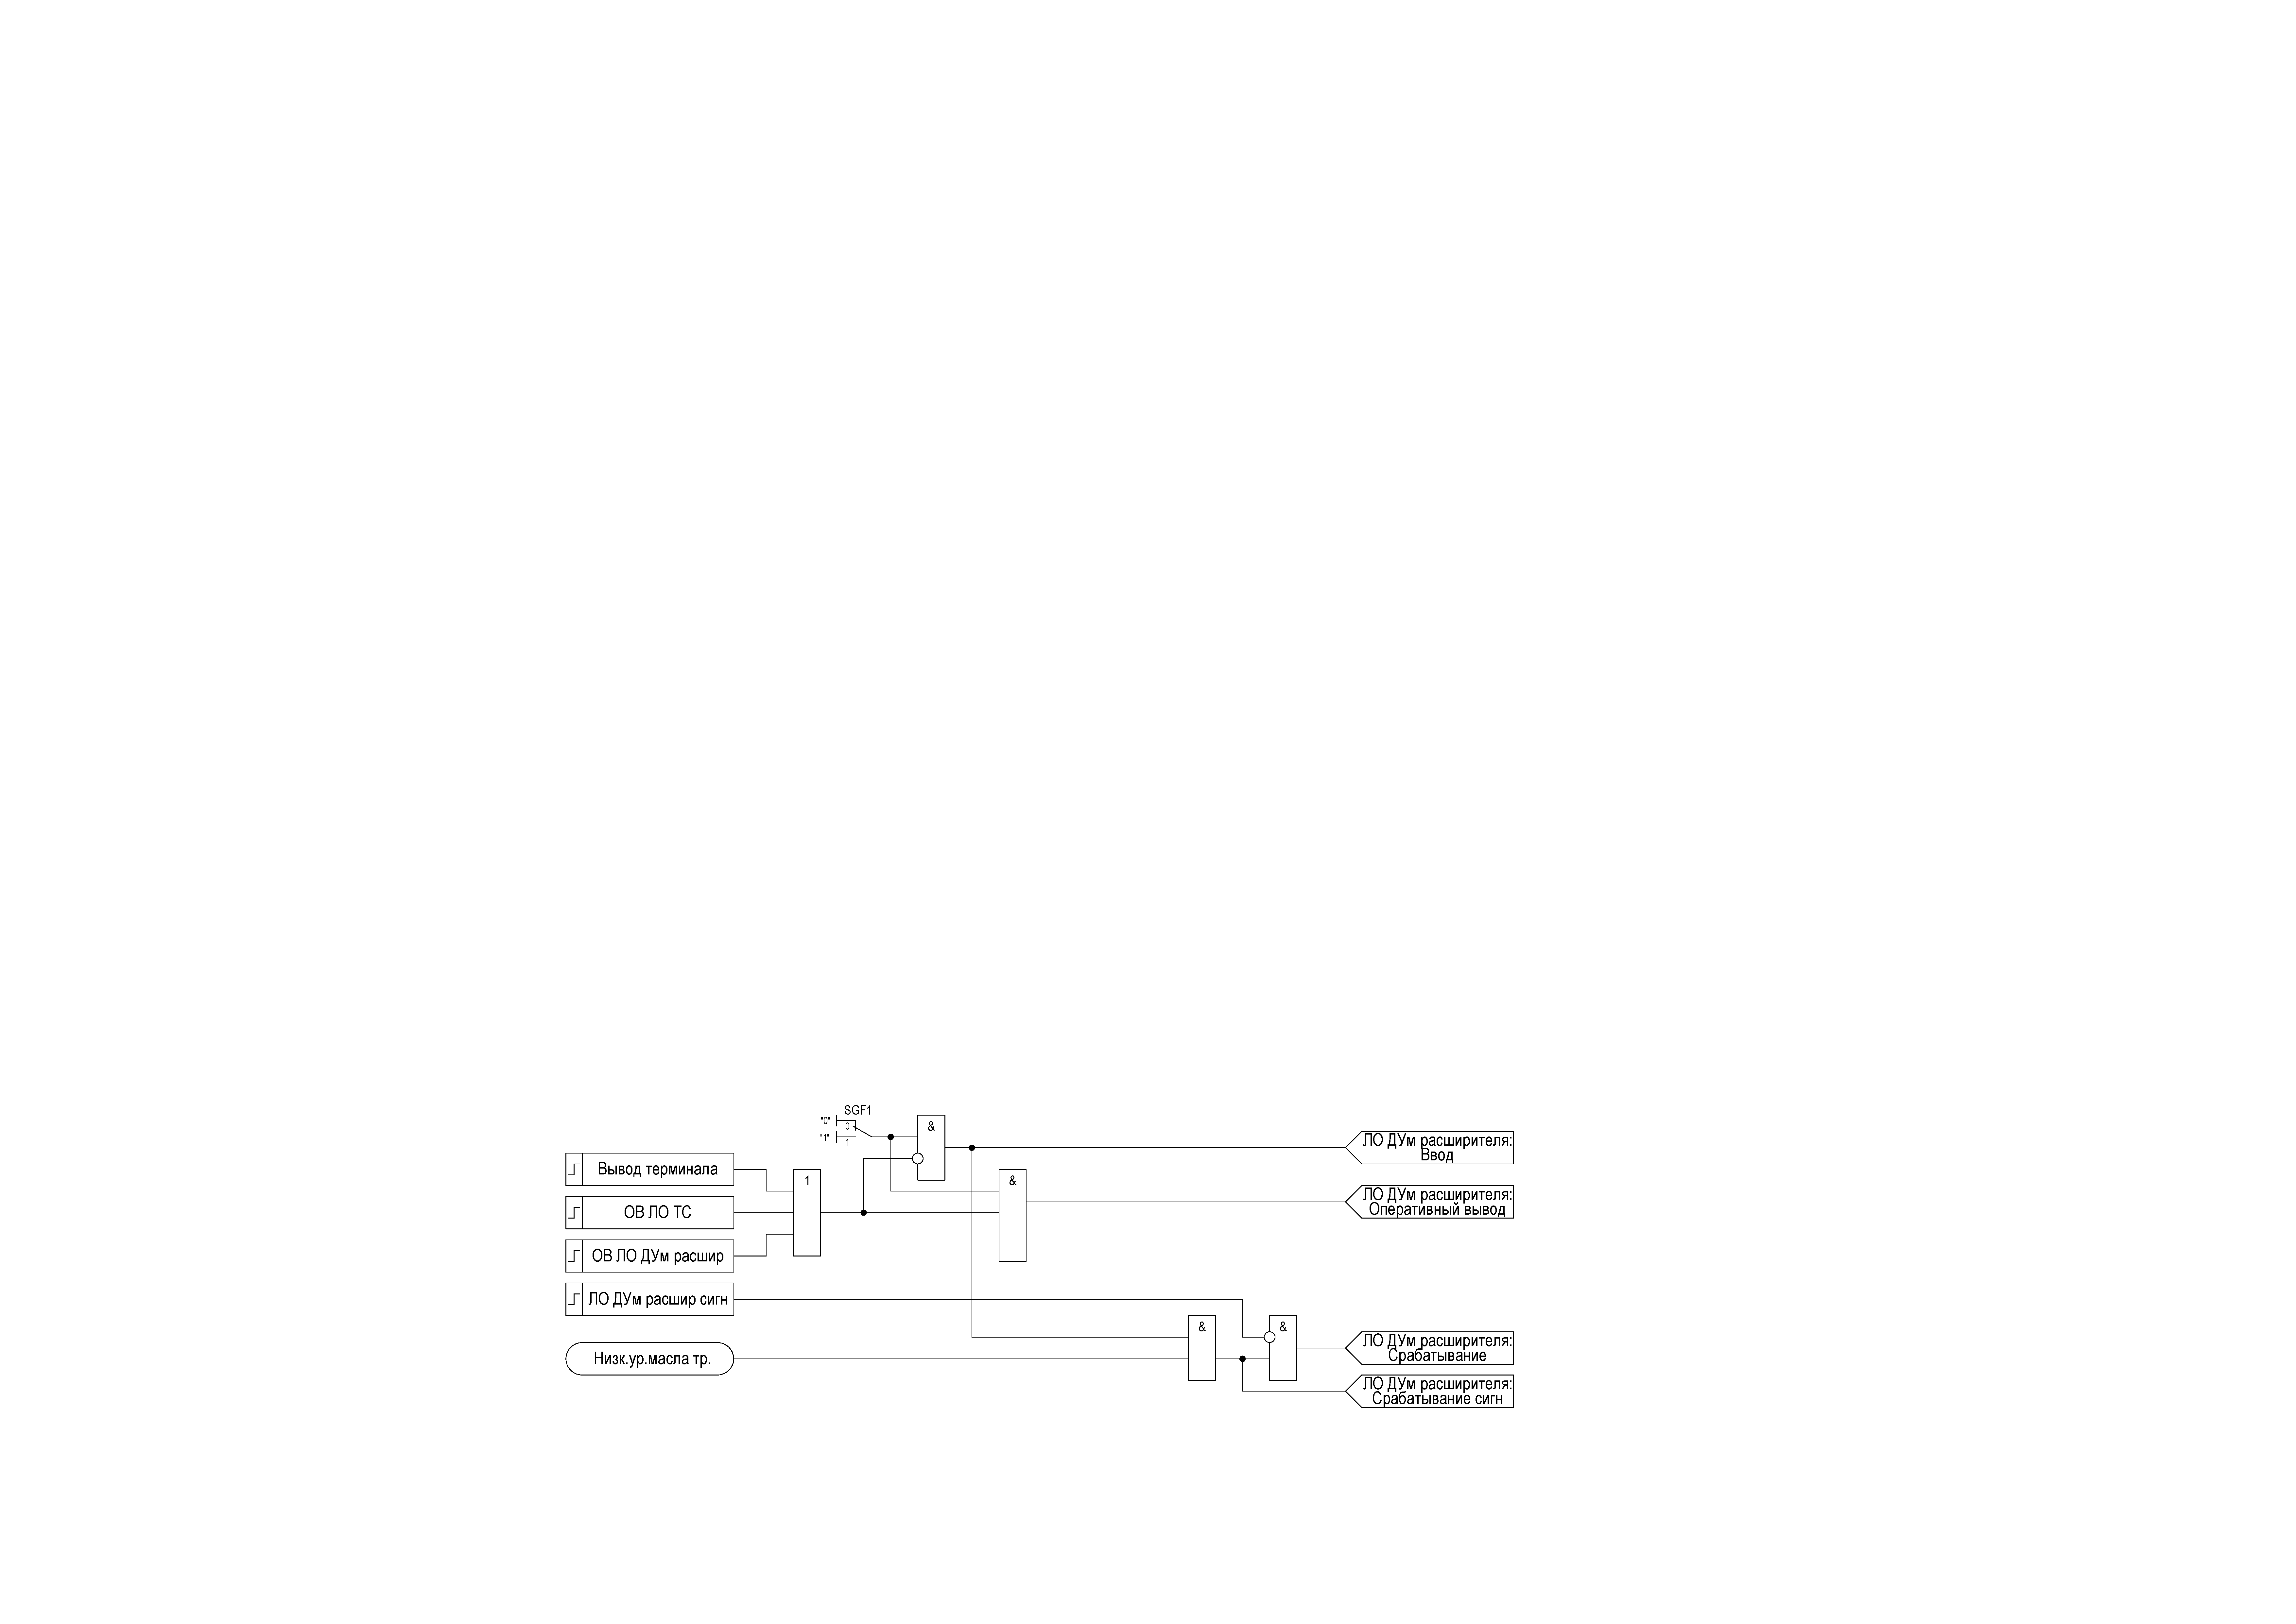
\includegraphics[width=1\textwidth,height=1\textheight,keepaspectratio]{img28.pdf}
\captionof{figure}{Функциональная схема <<ЛО~ДУм расширителя>>}\label{lotsdut:img1}
\end{figure}

\small
\begin{longtable}{|>{\centering\arraybackslash}m{5.3cm}|>{\centering\arraybackslash}m{3.3cm}|>{\centering\arraybackslash}m{4.2cm}|>{\centering\arraybackslash}m{1.8cm}|>{\centering\arraybackslash}m{1cm}|}
\caption{Параметры для настройки функции <<ЛО ДУм расширителя>>\hfill\vspace{-0.5\baselineskip}}\label{lotsdut:tbl1}\\ 
\hline
\rowcolor{gray!30}
Параметр (Параметр на ИЧМ) & Условное обозначение на схеме & Значение/ Диапазон & Единица измерения & Шаг \\ 
\hline
\endfirsthead
\caption*{\hspace{3pt}\emph{Продолжение таблицы \ref{lotsdut:tbl1}\hfill\vspace{-0.5\baselineskip}}} \\ % сделано по ГОСТ 2.105 п.6.8.7
\hline
\rowcolor{gray!30}
Параметр (Параметр на ИЧМ) & Условное обозначение на схеме & Значение/ Диапазон & Единица измерения & Шаг \\ 
\endhead
\endfoot
\endlastfoot
\centering Ввод функции в работу (Ввод\_функции) & \centering SGF1 & \centering 0 = Не предусмотрено\\1 = Предусмотрено & \centering -- & \centering \arraybackslash -- \\
\hline
\end{longtable}
\normalsize

\end{enumerate}

\end{enumerate}
\FloatBarrier % Все float'ы ДО этой строки будут размещены здесь.
\needspace{4\baselineskip}
\color{uniblue}{\subsection{Логика отключения трансформатора (ЛО Т)}}
\color{black}

\begin{enumerate}[label=\arabic{section}.\arabic{subsection}.\arabic{enumi}, labelsep=4pt, leftmargin=0pt, itemindent=57pt, itemsep=0pt, parsep=5pt] % если что можно крутить itemsep

\item Общие сведения

\begin{enumerate}[label=\arabic{section}.\arabic{subsection}.\arabic{enumi}.\arabic*, labelsep=4pt, leftmargin=0em, itemindent=65pt, parsep=0pt]

\item
Функциональный блок <<ЛО Т>> принимает сигналы срабатывания защитных функций трансформатора в составе устройства и сигналов отключения от некоторых внешних устройств РЗ (действующих на отключение трансформатора со всех сторон с запретом АПВ) и формирует общие сигналы отключения трансформатора и запрета АПВ выключателей сторон трансформатора.
\item
Функциональный блок <<ЛО~Т>> может быть выведен из работы оперативно путем активации сигнала <<ОВ~ЛО~Т>>.

\end{enumerate}

\item Логика отключения трансформатора (ЛО)

\begin{enumerate}[label=\arabic{section}.\arabic{subsection}.\arabic{enumi}.\arabic*, labelsep=4pt, leftmargin=0em, itemindent=65pt, parsep=0pt]

\item
Ввод функции <<ЛО>> в работу на этапе параметрирования устройства осуществляется программным переключателем SGF1 <<Ввод\_функции>>. Информация о введенной функции отображается выходным сигналом <<ЛО Т / ЛО: Ввод>>.
\item
Функция <<ЛО>> может быть выведена из работы оперативно путем активации сигнала <<ОВ ЛО Т / ЛО>>, что характеризуется активным состоянием сигнала <<ЛО Т / ЛО: Оперативный вывод>> на выходе функции.
\item
При появлении сигналов срабатывания от защитных функций в составе устройства или сигнала отключения от внешней автоматики охлаждения функция формирует сигнал <<ЛО Т / ЛО: Срабатывание>>.
\item
Алгоритм работы <<ЛО>> выполнен в соответствии с рисунком \ref{loobsh:img1}. В таблице \ref{loobsh:tbl1} приведены параметры, необходимые для настройки функции <<ЛО>>.

\vspace{3mm}
\begin{figure}[!h]
\centering
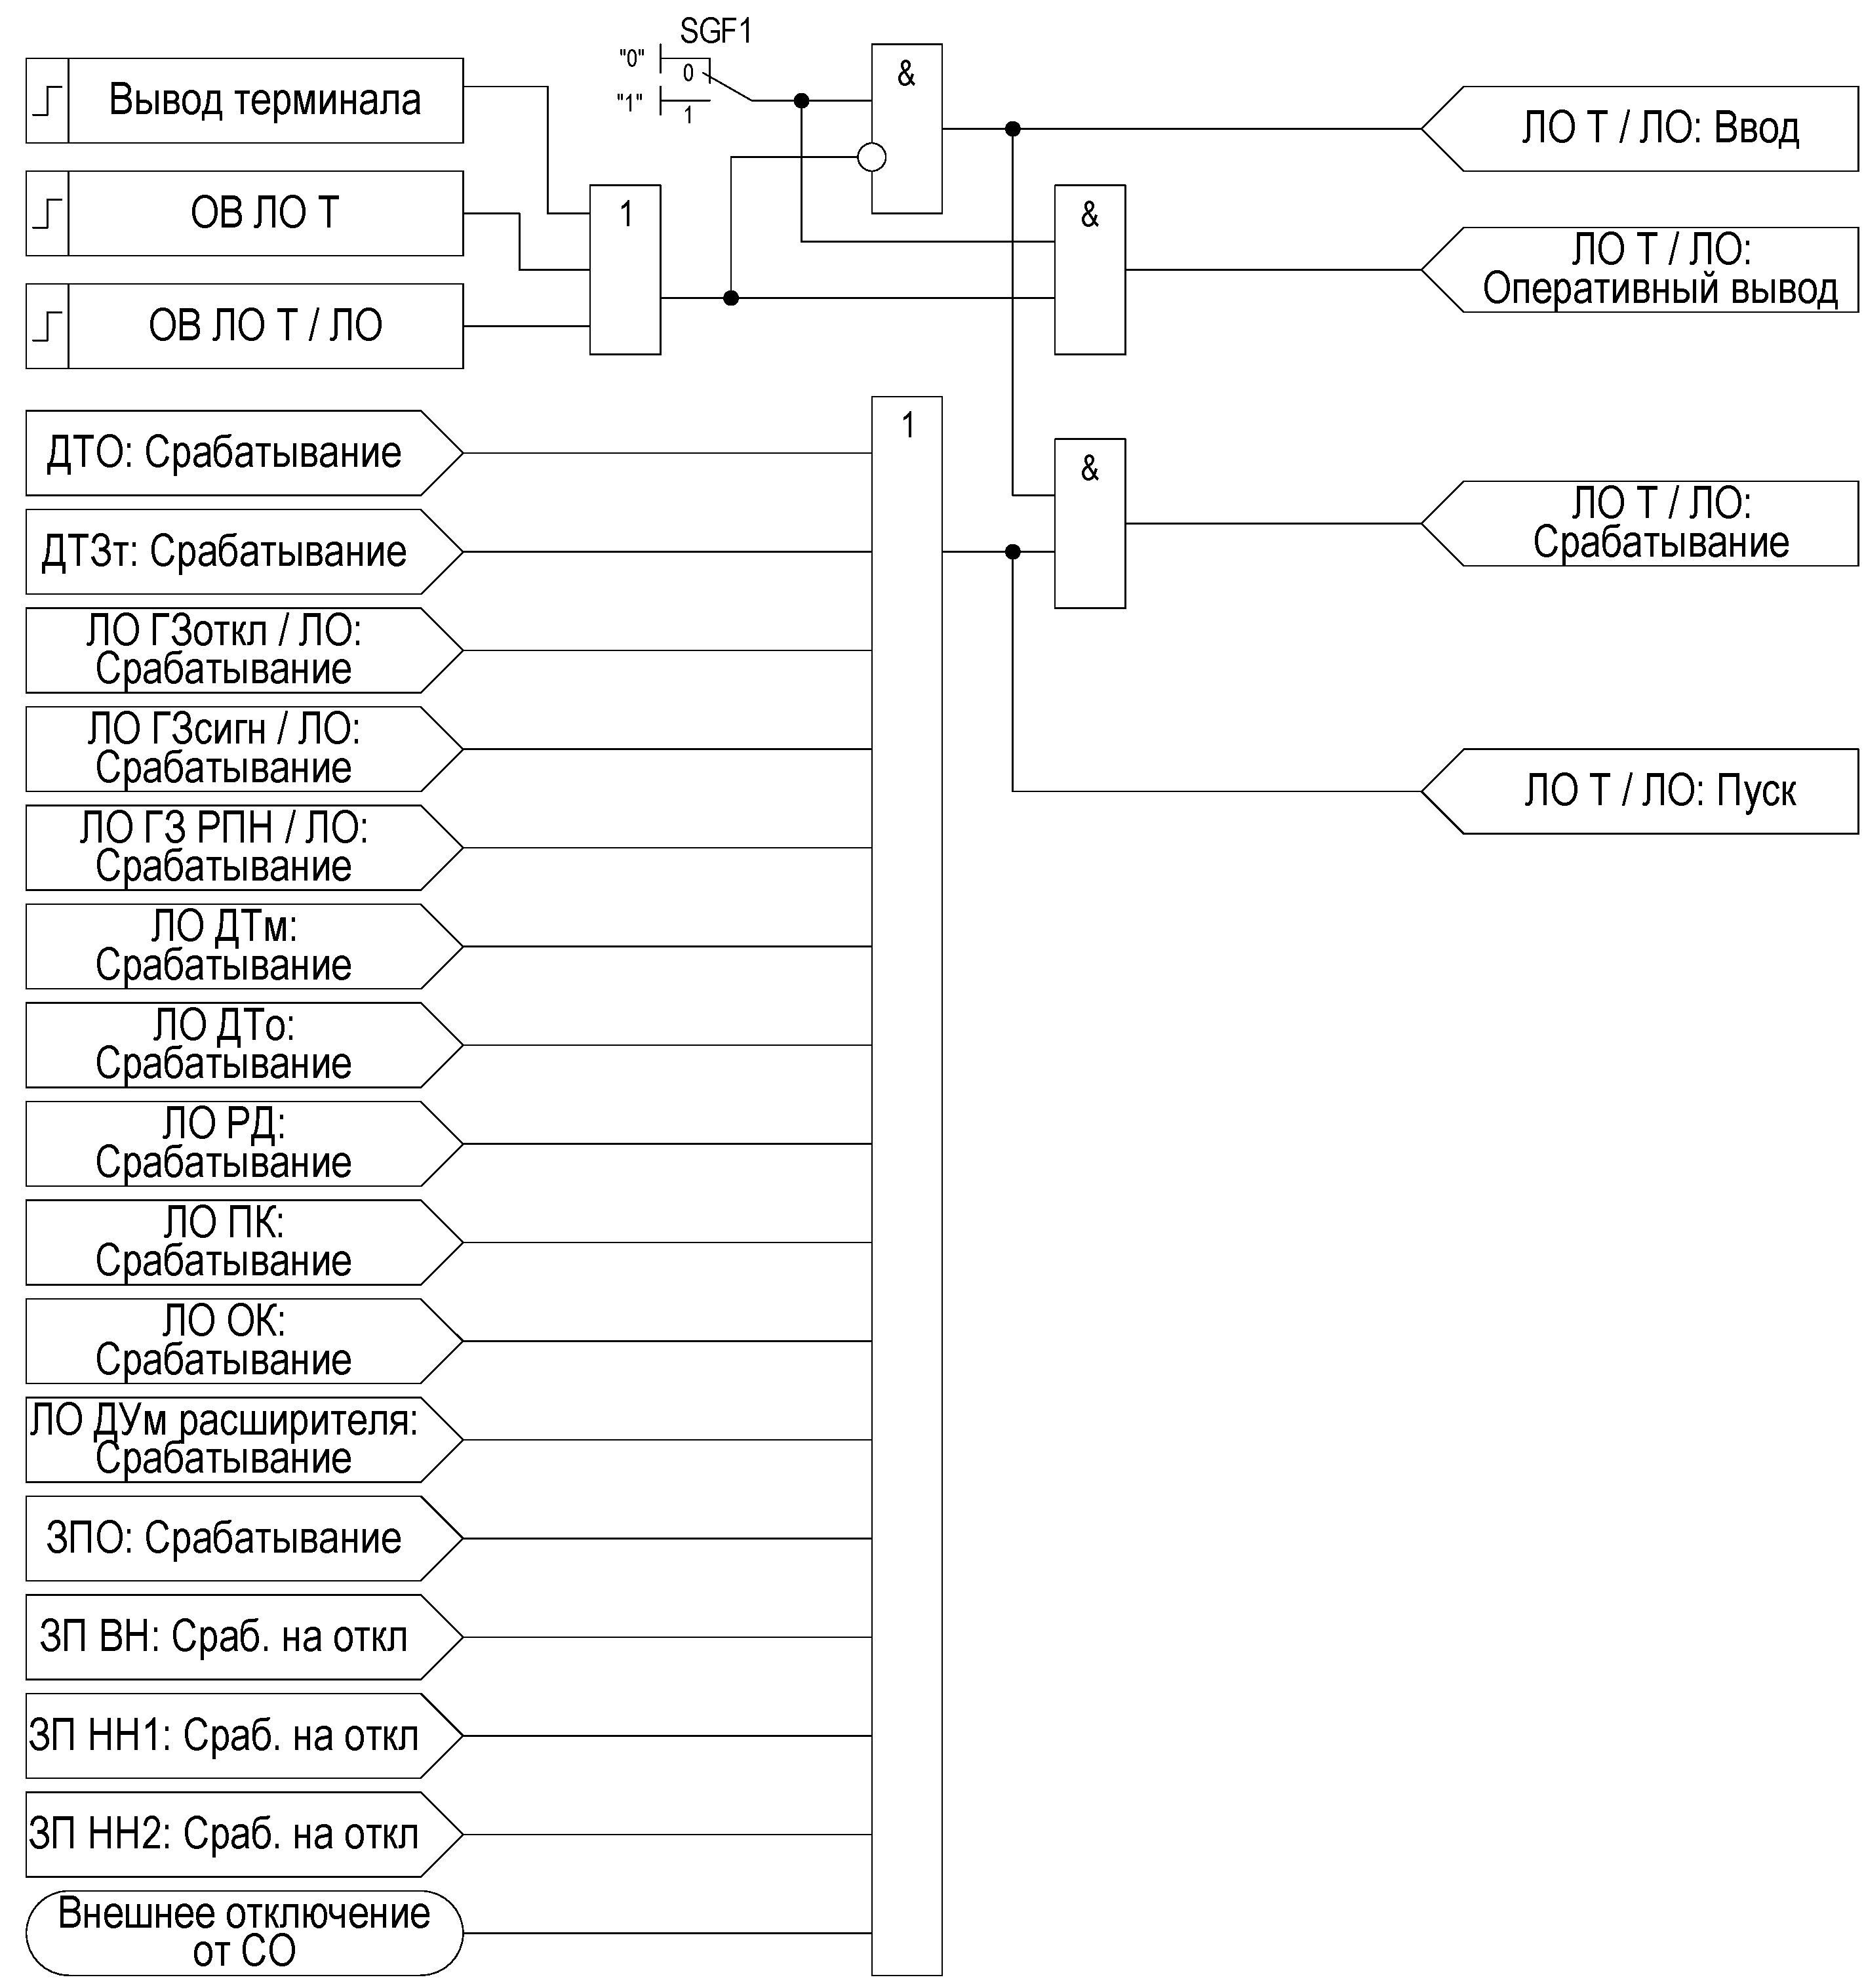
\includegraphics[width=0.9\textwidth,height=0.9\textheight,keepaspectratio]{img29.pdf}
\captionof{figure}{Функциональная схема <<ЛО>>}\label{loobsh:img1}
\end{figure}

\small
\begin{longtable}{|>{\centering\arraybackslash}m{5.3cm}|>{\centering\arraybackslash}m{3.3cm}|>{\centering\arraybackslash}m{4.2cm}|>{\centering\arraybackslash}m{1.8cm}|>{\centering\arraybackslash}m{1cm}|}
\caption{Параметры для настройки функции <<ЛО>>\hfill\vspace{-0.5\baselineskip}}\label{loobsh:tbl1}\\ 
\hline
\rowcolor{gray!30}
Параметр (Параметр на ИЧМ) & Условное обозначение на схеме & Значение/ Диапазон & Единица измерения & Шаг \\ 
\hline
\endfirsthead
\caption*{\hspace{3pt}\emph{Продолжение таблицы \ref{loobsh:tbl1}\hfill\vspace{-0.5\baselineskip}}} \\ % сделано по ГОСТ 2.105 п.6.8.7
\hline
\rowcolor{gray!30}
Параметр (Параметр на ИЧМ) & Условное обозначение на схеме & Значение/ Диапазон & Единица измерения & Шаг \\ 
\endhead
\endfoot
\endlastfoot
\centering Ввод функции в работу (Ввод\_функции) & \centering SGF1 & \centering 0 = Не предусмотрено\\1 = Предусмотрено & \centering -- & \centering \arraybackslash -- \\
\hline
\end{longtable}
\normalsize

\end{enumerate}
\FloatBarrier % Все float'ы ДО этой строки будут размещены здесь.

\item Логика запрета АПВ выключателей трансформатора (ЗАПВ)

\begin{enumerate}[label=\arabic{section}.\arabic{subsection}.\arabic{enumi}.\arabic*, labelsep=4pt, leftmargin=0em, itemindent=65pt, parsep=0pt]

\item
Ввод функции <<Запрет АПВ>> в работу на этапе параметрирования устройства  осуществляется программным переключателем SGF1 <<Ввод\_функции>>. Информация о введенной функции отображается выходным сигналом <<ЛО Т / ЗАПВ: Ввод>>.
\item
Функция <<Запрет АПВ>> может быть выведена из работы оперативно путем активации сигнала <<ОВ ЛО Т / ЗАПВ>>, что характеризуется активным состоянием сигнала <<ЛО Т / ЗАПВ: Оперативный вывод>> на выходе функции.
\item
Функция принимает сигнал срабатывания от общей логики отключения и формирует сигнал <<ЛО Т / ЗАПВ: Запрет АПВ>>. 
Алгоритм работы <<Запрет АПВ>> выполнен в соответствии с рисунком \ref{zapvvnutr:img2}. В таблице \ref{zapvvnutr:tbl2} приведены параметры, необходимые для настройки функции <<Запрет АПВ>>.

\begin{figure}[!h]
\centering
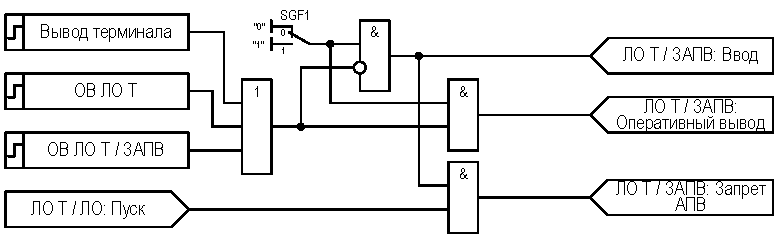
\includegraphics[width=0.9\textwidth,height=0.9\textheight,keepaspectratio]{img30.pdf}
\captionof{figure}{Функциональная схема <<ЗАПВ>>}\label{zapvvnutr:img2}
\end{figure}

\small
\begin{longtable}{|>{\centering\arraybackslash}m{5.3cm}|>{\centering\arraybackslash}m{3.3cm}|>{\centering\arraybackslash}m{4.2cm}|>{\centering\arraybackslash}m{1.8cm}|>{\centering\arraybackslash}m{1cm}|}
\caption{Параметры для настройки функции <<ЗАПВ>>\hfill\vspace{-0.5\baselineskip}}\label{zapvvnutr:tbl2}\\ 
\hline
\rowcolor{gray!30}
Параметр (Параметр на ИЧМ) & Условное обозначение на схеме & Значение/ Диапазон & Единица измерения & Шаг \\ 
\hline
\endfirsthead
\caption*{\hspace{3pt}\emph{Продолжение таблицы \ref{zapvvnutr:tbl2}\hfill\vspace{-0.5\baselineskip}}} \\ % сделано по ГОСТ 2.105 п.6.8.7
\hline
\rowcolor{gray!30}
Параметр (Параметр на ИЧМ) & Условное обозначение на схеме & Значение/ Диапазон & Единица измерения & Шаг \\ 
\endhead
\endfoot
\endlastfoot
\centering Ввод функции в работу (Ввод\_функции) & \centering SGF1 & \centering 0 = Не предусмотрено\\1 = Предусмотрено & \centering -- & \centering \arraybackslash -- \\
\hline
\end{longtable}
\normalsize

\end{enumerate}

\end{enumerate}
\FloatBarrier % Все float'ы ДО этой строки будут размещены здесь.
\needspace{3\baselineskip}
\color{uniblue}{\subsection{Логика отключения выключателя стороны ВН трансформатора (ЛО ВН)}}
\color{black}

\begin{enumerate}[label=\arabic{section}.\arabic{subsection}.\arabic*, labelsep=4pt, leftmargin=0pt, itemindent=57pt]

\item
Функциональный блок <<ЛО ВН>> служит для формирования команды отключения выключателя стороны ВН трансформатора (посредством функции <<ЛО>>) от защит в составе устройства и внешних защит, которые действуют через данное микропроцессорное устройство. 
\item
Функция <<ЛО>> (логика отключения выключателя стороны ВН трансформатора) входит в состав функционального блока <<ЛО ВН>>.
\item
Ввод функции <<ЛО>> в работу на этапе параметрирования устройства осуществляется программным переключателем SGF1 <<Ввод\_функции>>. Информация о введенной функции отображается выходным сигналом <<ЛО ВН / ЛО: Ввод>>.
\item
Функция <<ЛО>> может быть выведена из работы оперативно путем активации сигнала <<ОВ ЛО ВН>>, что характеризуется активным состоянием сигнала <<ЛО ВН / ЛО: Оперативный вывод>> на выходе функции.
\item
При появлении синалов срабатывания от общей логики отключения трансформатора и внешних устройств РЗА сторон НН функция формирует сигналы <<Отключение>> и <<Отключить аварийно>>, сигнал <<Отключить аварийно>> является импульсным, время импульса определяется выдержкой времени таймера T1 (уставка <<Тимп>>). 
Алгоритм работы <<ЛО>> выполнен в соответствии с рисунком \ref{lovn:img1}. В таблице \ref{lovn:tbl1} приведены параметры, необходимые для настройки функции <<ЛО>>.

\small
\begin{longtable}{|>{\centering\arraybackslash}m{5.3cm}|>{\centering\arraybackslash}m{3.3cm}|>{\centering\arraybackslash}m{4.2cm}|>{\centering\arraybackslash}m{1.8cm}|>{\centering\arraybackslash}m{1cm}|}
\caption{Параметры для настройки функции <<ЛО>>\hfill\vspace{-0.5\baselineskip}}\label{lovn:tbl1}\\ 
\hline
\rowcolor{gray!30}
Параметр (Параметр на ИЧМ) & Условное обозначение на схеме & Значение/ Диапазон & Единица измерения & Шаг \\ 
\hline
\endfirsthead
\caption*{\hspace{3pt}\emph{Продолжение таблицы \ref{lovn:tbl1}\hfill\vspace{-0.5\baselineskip}}} \\ % сделано по ГОСТ 2.105 п.6.8.7
\hline
\rowcolor{gray!30}
Параметр (Параметр на ИЧМ) & Условное обозначение на схеме & Значение/ Диапазон & Единица измерения & Шаг \\ 
\endhead
\endfoot
\endlastfoot
\centering Ввод функции в работу (Ввод\_функции) & \centering SGF1 & \centering 0 = Не предусмотрено\\1 = Предусмотрено & \centering -- & \centering \arraybackslash -- \\
\hline
\centering Длительность импульса (Тимп) & \centering T1 & \centering 0,05 ... 60,00 & \centering с & \centering \arraybackslash 0,01 \\
\hline
\end{longtable}
\normalsize

\vspace{3mm}
\begin{figure}[!h]
\centering
\ifboolexpr{bool {isT}}
{
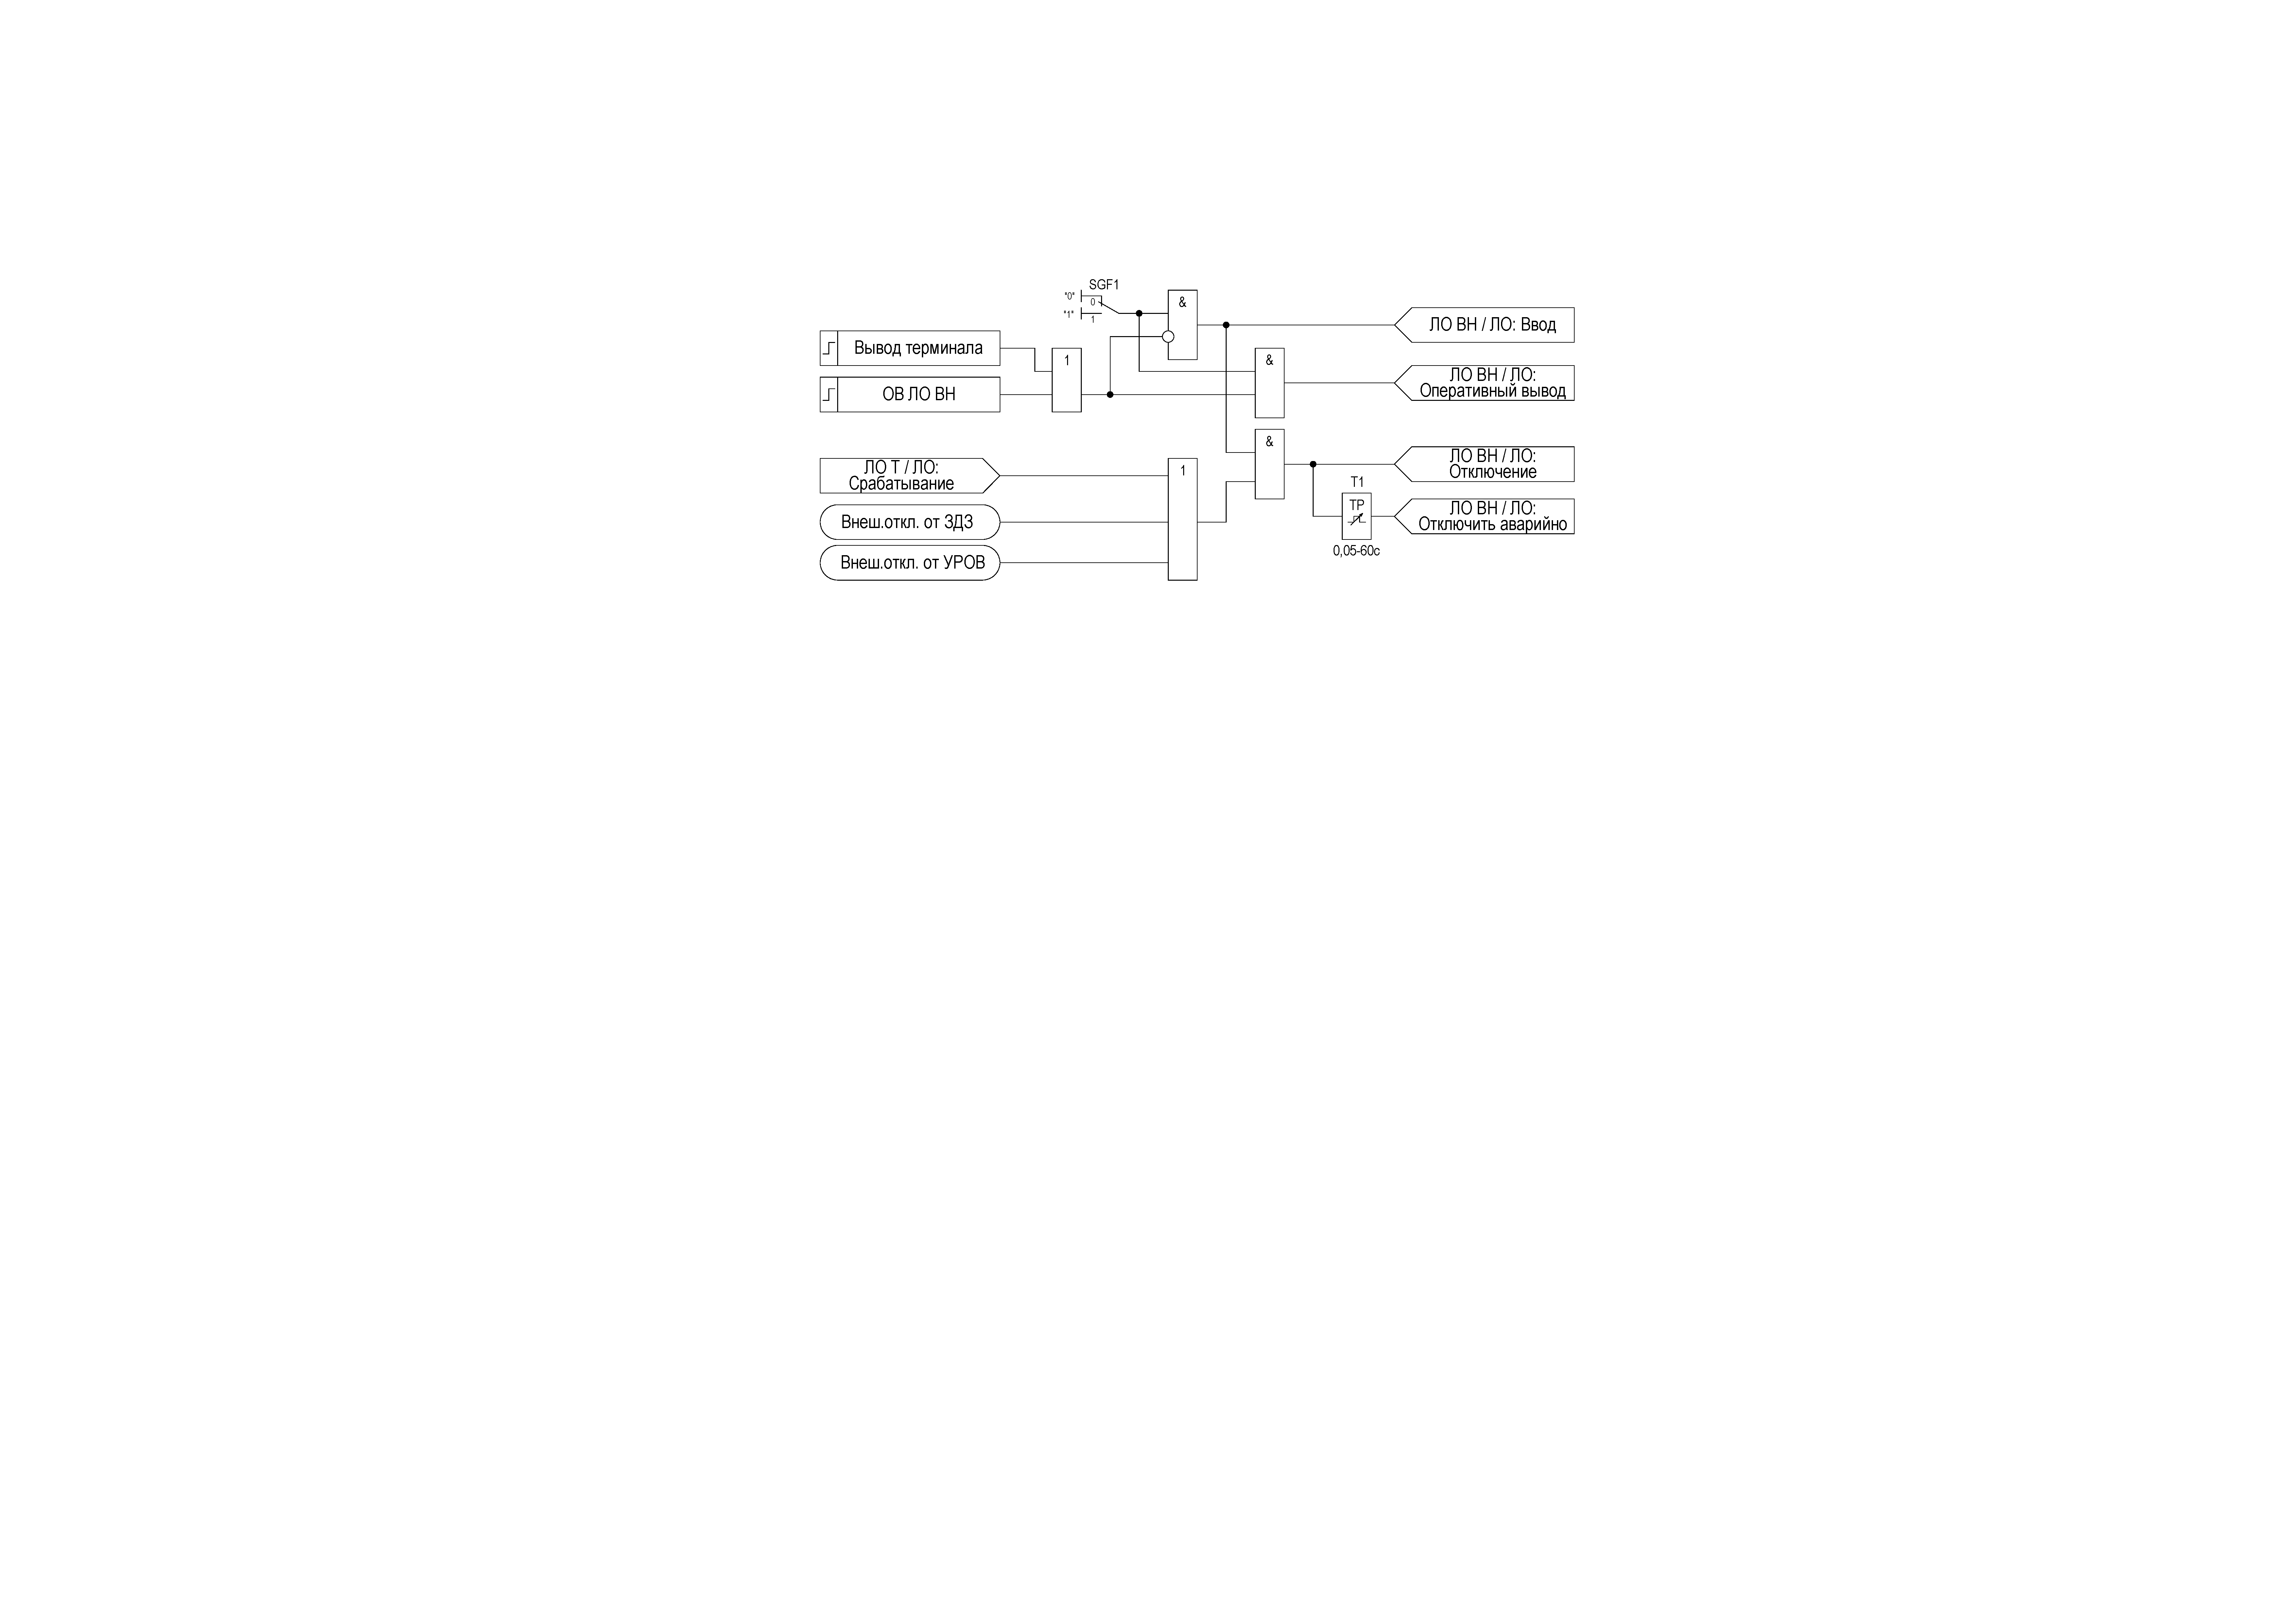
\includegraphics[width=0.85\textwidth,height=0.85\textheight,keepaspectratio]{img31.pdf}
}{}
\ifboolexpr{bool {isDZT2}}
{
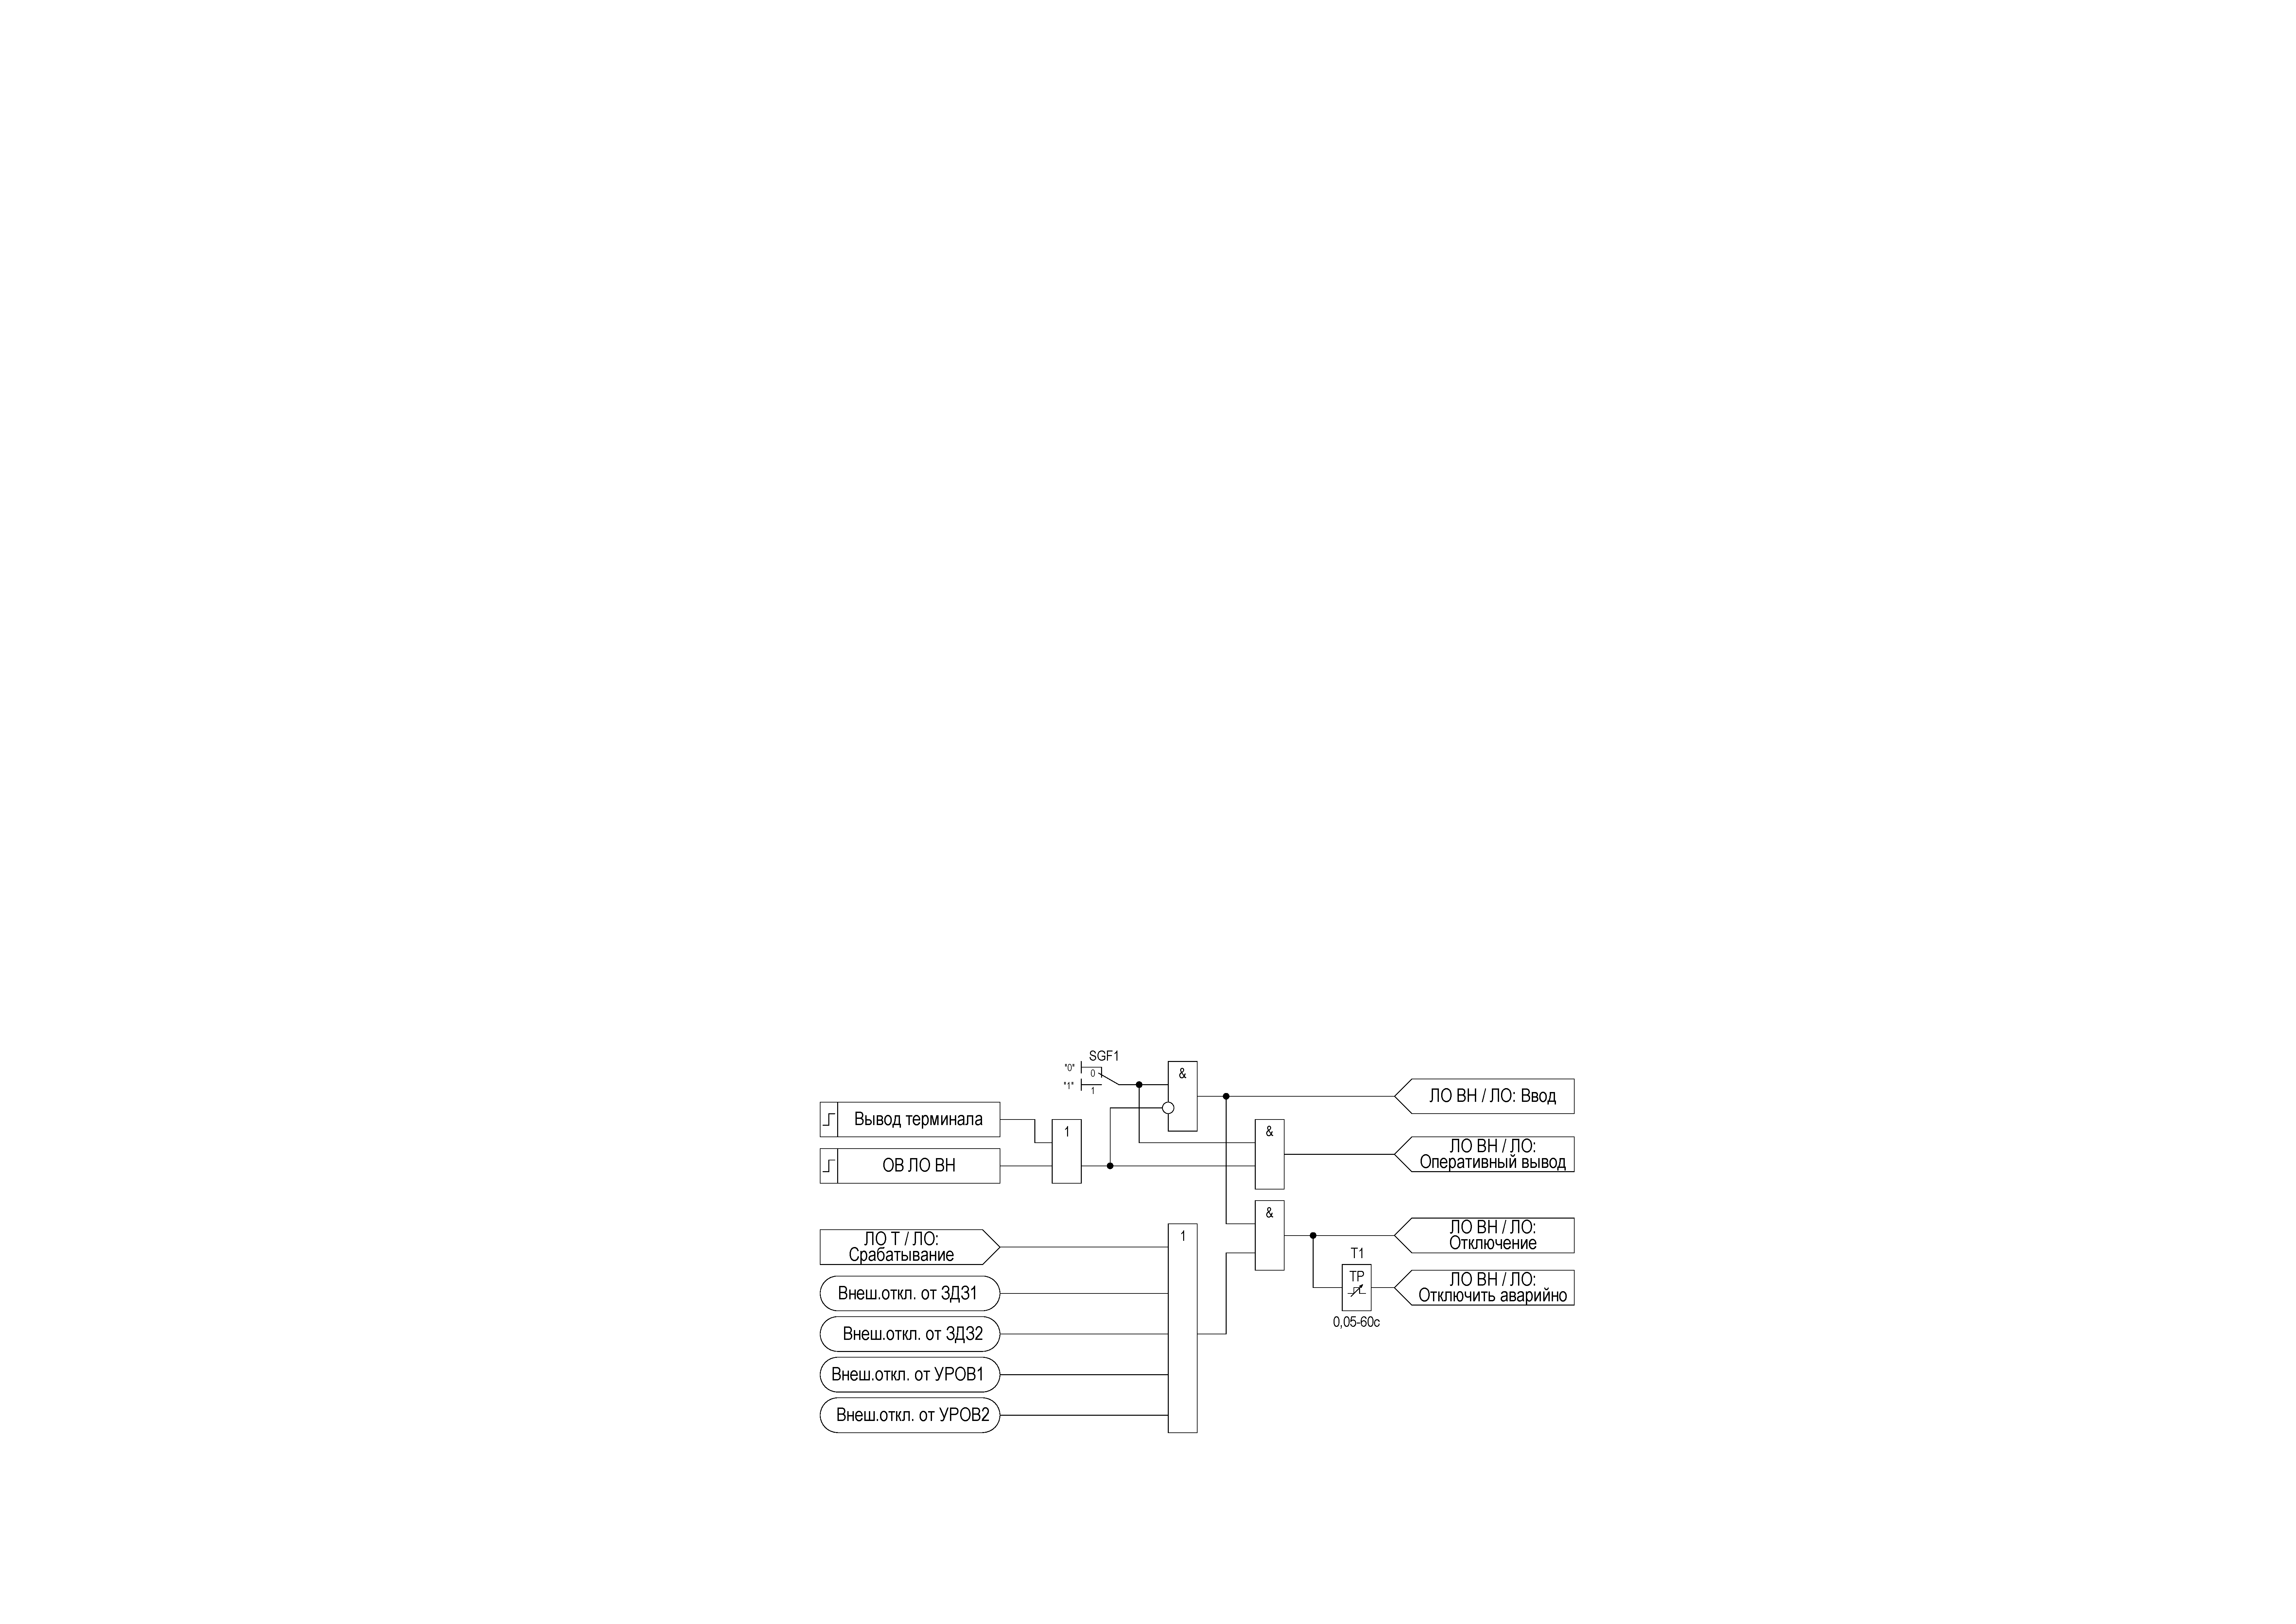
\includegraphics[width=0.85\textwidth,height=0.85\textheight,keepaspectratio]{img32.pdf}
}{}
\ifboolexpr{bool {isT2}}
{
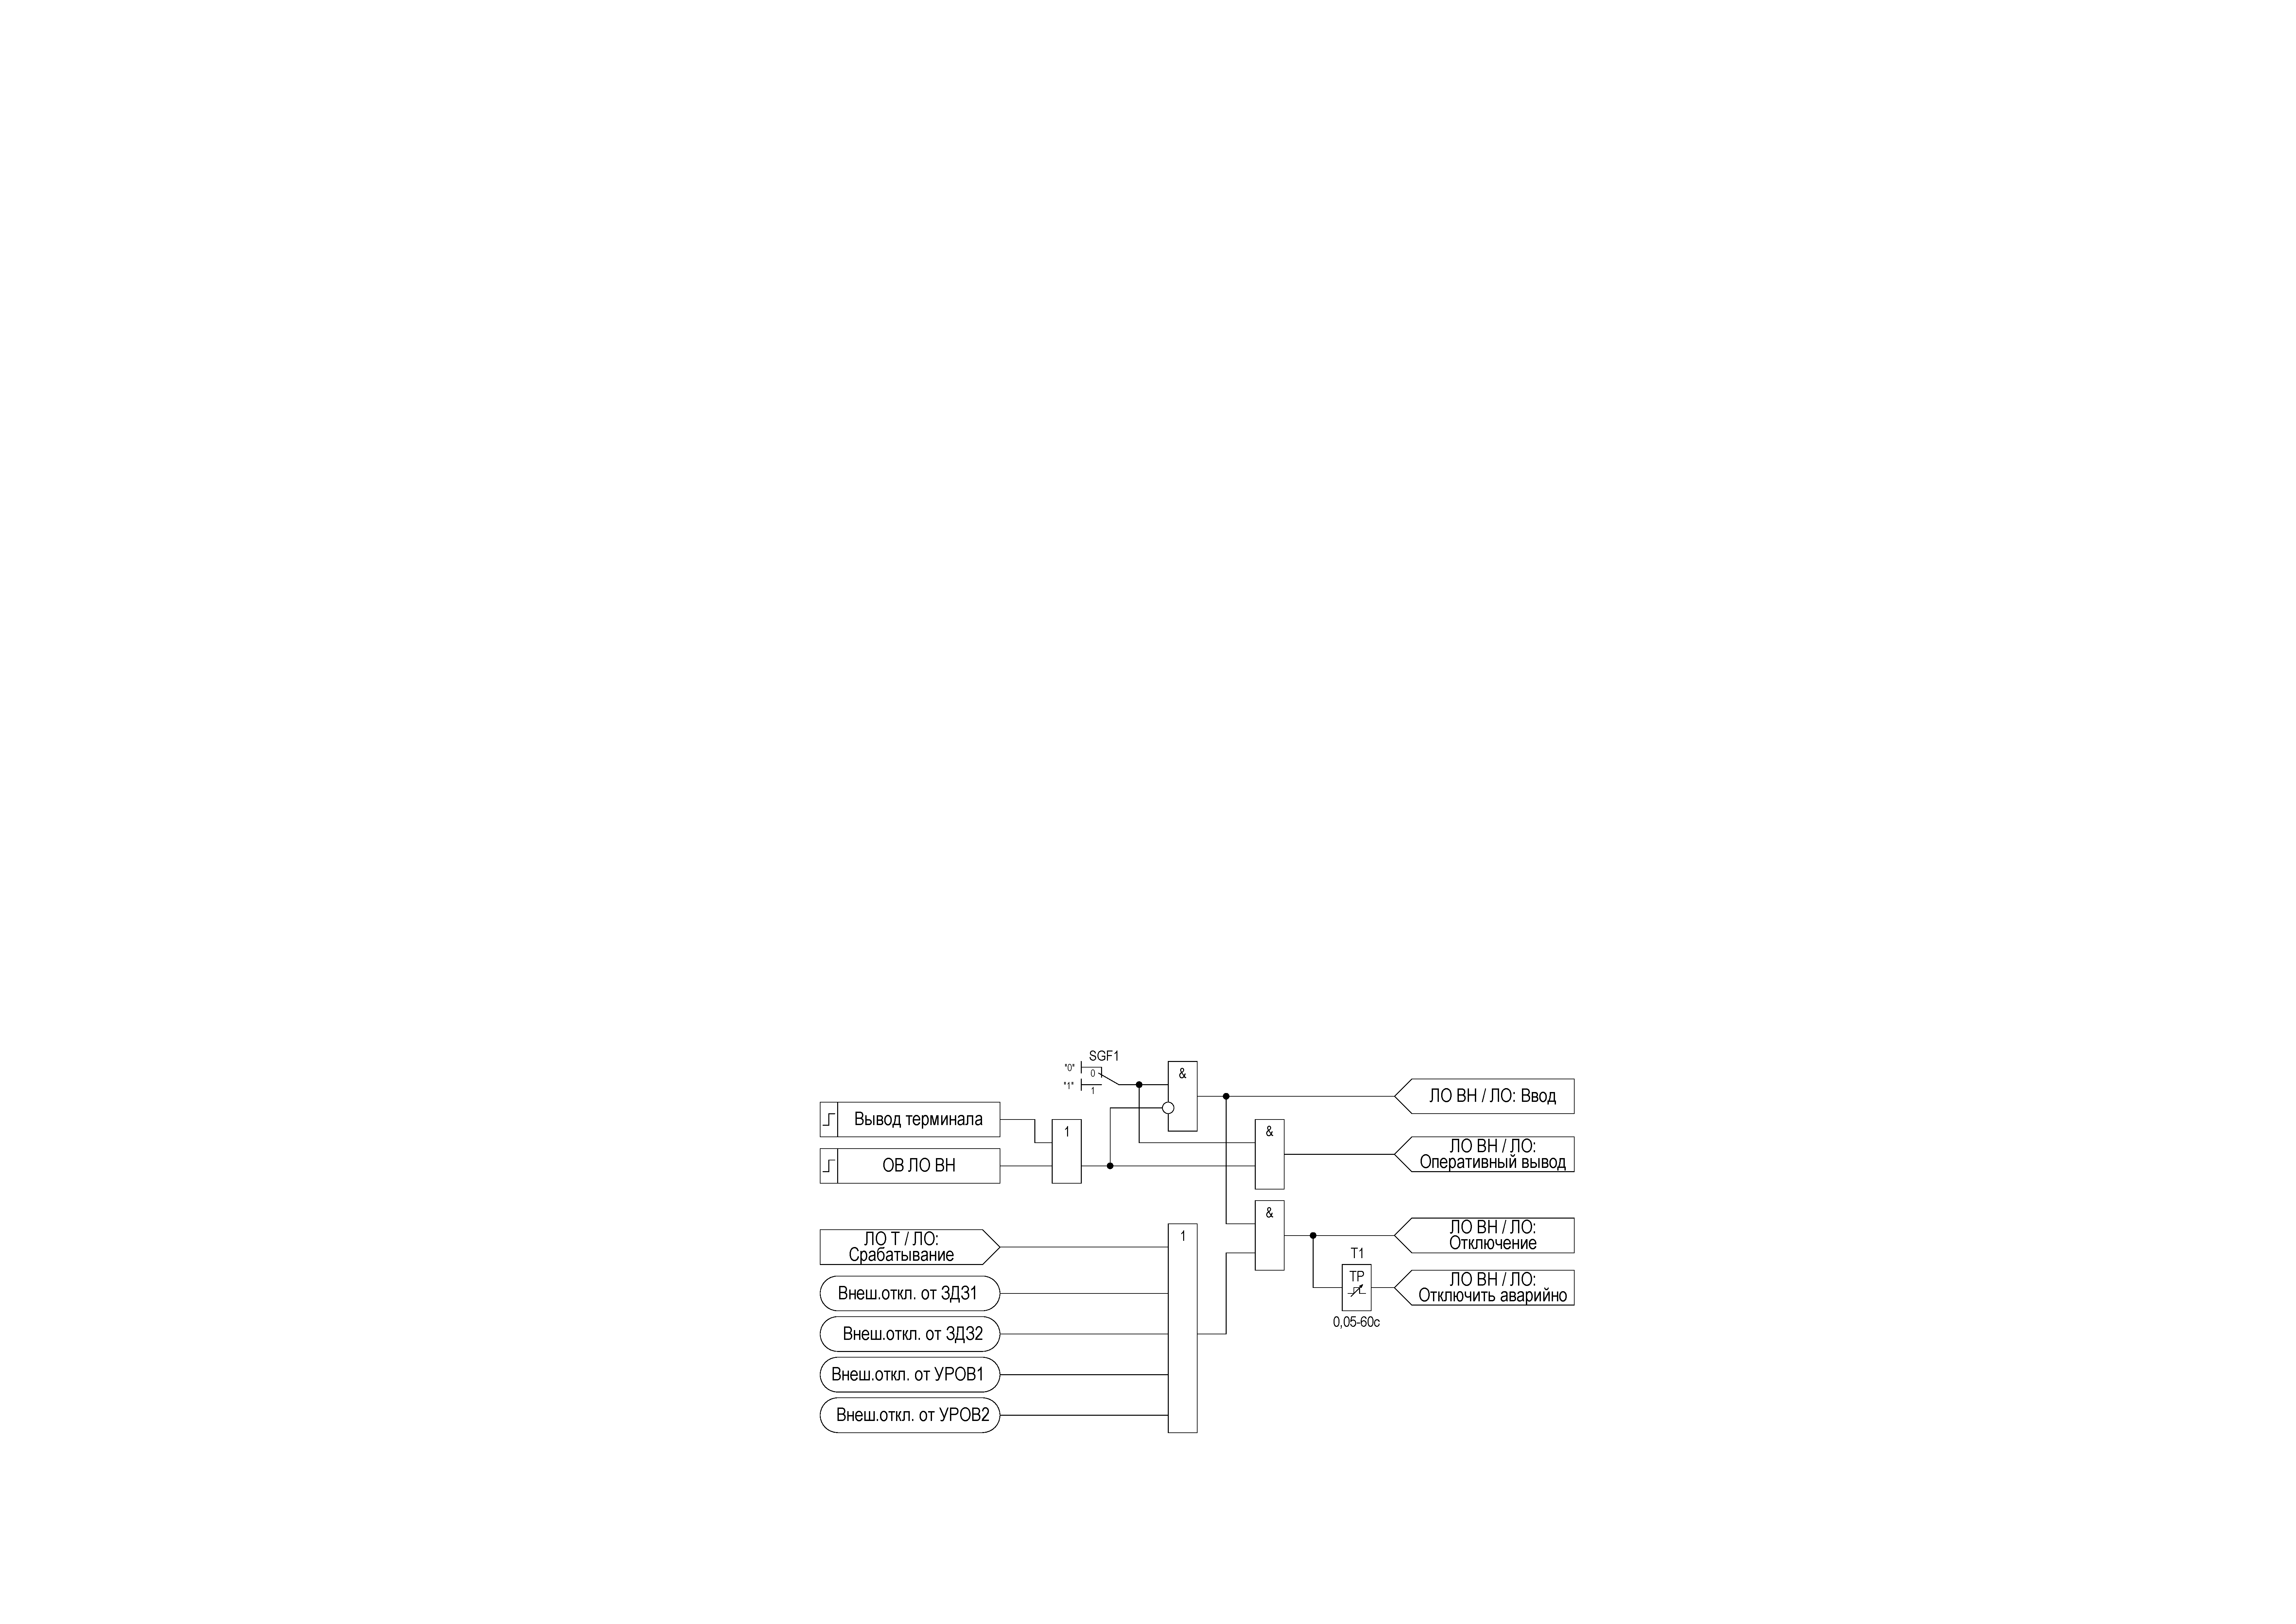
\includegraphics[width=0.85\textwidth,height=0.85\textheight,keepaspectratio]{img33.pdf}
}{}

\captionof{figure}{Функциональная схема <<ЛО>>}\label{lovn:img1}
\end{figure}

\end{enumerate}
\FloatBarrier % Все float'ы ДО этой строки будут размещены здесь.


\needspace{3\baselineskip}
\color{uniblue}{\subsection{Логика отключения выключателя стороны НН трансформатора (ЛО НН)}}
\color{black}

\begin{enumerate}[label=\arabic{section}.\arabic{subsection}.\arabic{enumi}, labelsep=4pt, leftmargin=0pt, itemindent=57pt, itemsep=0pt, parsep=5pt] % если что можно крутить itemsep


\item Общие сведения

\begin{enumerate}[label=\arabic{section}.\arabic{subsection}.\arabic{enumi}.\arabic*, labelsep=4pt, leftmargin=0em, itemindent=65pt, parsep=0pt]

\item
Функциональный блок <<ЛО НН>> служит для формирования команды отключения в схему выключателя ввода секций НН трансформатора (посредством функции <<ЛО>>) и команды запрета АПВ (посредством функции <<ЗАПВ>>) в схему АПВ выключателя ввода секции НН от защит в составе устройства и внешних защит, которые действуют через данное микропроцессорное устройство.
\item 
В составе устройства предусматривается две логики отключения стороны НН трансформатора (для схем управления вводными выключателелями секций НН1 и НН2): <<ЛО НН1>> и <<ЛО НН2>>.
\item
Функциональный блок <<ЛО НН>> может быть выведен из работы оперативно путем активации сигнала <<ОВ~ЛО~НН>>.

\end{enumerate}


\item Логика отключения выключателя ввода стороны НН (ЛО)

\begin{enumerate}[label=\arabic{section}.\arabic{subsection}.\arabic{enumi}.\arabic*, labelsep=4pt, leftmargin=0em, itemindent=65pt, parsep=0pt]

\item
Ввод функции <<ЛО>> в работу на этапе параметрирования устройства осуществляется программным переключателем SGF1 <<Ввод\_функции>>. Информация о введенной функции отображается выходным сигналом <<ЛО НН / ЛО: Ввод>>.
\item
Функция <<ЛО>> может быть выведена из работы оперативно путем активации сигнала <<ОВ ЛО НН / ЛО>>, что характеризуется активным состоянием сигнала <<ЛО НН / ЛО: Оперативный вывод>> на выходе функции.  
\item
Функция принимает сигнал срабатывания от общей логики отключения трансформатора и формирует сигналы <<ЛО НН / ЛО: Отключение>> и <<ЛО НН / ЛО: Отключить аварийно>>, сигнал <<ЛО НН / ЛО: Отключить аварийно>> является импульсным, время импульса определяется выдержкой времени таймера T1 (уставка <<Тимп>>).
\item
Алгоритм работы <<ЛО>> выполнен в соответствии с рисунком \ref{lonn:img1}. В таблице \ref{lonn:tbl1} приведены параметры, необходимые для настройки функции <<ЛО>>.

\vspace{3mm}
\begin{figure}[!h]
\centering
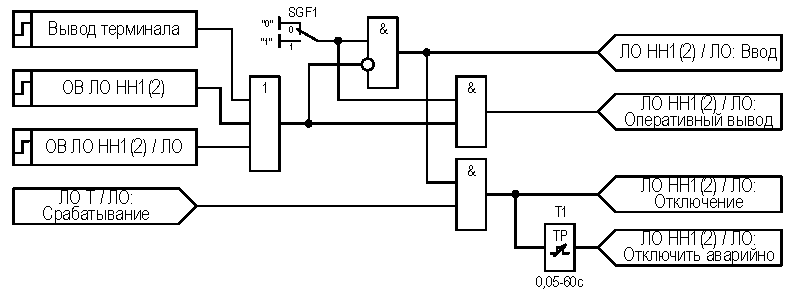
\includegraphics[width=0.9\textwidth,height=0.9\textheight,keepaspectratio]{img34.pdf}
\captionof{figure}{Функциональная схема <<ЛО>>}\label{lonn:img1}
\end{figure}

\small
\begin{longtable}{|>{\centering\arraybackslash}m{5.3cm}|>{\centering\arraybackslash}m{3.3cm}|>{\centering\arraybackslash}m{4.2cm}|>{\centering\arraybackslash}m{1.8cm}|>{\centering\arraybackslash}m{1cm}|}
\caption{Параметры для настройки функции <<ЛО>>\hfill\vspace{-0.5\baselineskip}}\label{lonn:tbl1}\\ 
\hline
\rowcolor{gray!30}
Параметр (Параметр на ИЧМ) & Условное обозначение на схеме & Значение/ Диапазон & Единица измерения & Шаг \\ 
\hline
\endfirsthead
\caption*{\hspace{3pt}\emph{Продолжение таблицы \ref{lonn:tbl1}\hfill\vspace{-0.5\baselineskip}}} \\ % сделано по ГОСТ 2.105 п.6.8.7
\hline
\rowcolor{gray!30}
Параметр (Параметр на ИЧМ) & Условное обозначение на схеме & Значение/ Диапазон & Единица измерения & Шаг \\ 
\endhead
\endfoot
\endlastfoot
\centering Ввод функции в работу (Ввод\_функции) & \centering SGF1 & \centering 0 = Не предусмотрено\\1 = Предусмотрено & \centering -- & \centering \arraybackslash -- \\
\hline
\centering Длительность импульса (Тимп) & \centering T1 & \centering 0,05 ... 60,00 & \centering с & \centering \arraybackslash 0,01 \\
\hline
\end{longtable}
\normalsize

\end{enumerate}
\FloatBarrier % Все float'ы ДО этой строки будут размещены здесь.

\item Логика запрета АПВ выключателя ввода стороны НН (Запрет АПВ)

\begin{enumerate}[label=\arabic{section}.\arabic{subsection}.\arabic{enumi}.\arabic*, labelsep=4pt, leftmargin=0em, itemindent=65pt, parsep=0pt]

\item
Ввод функции <<Запрет АПВ>> в работу на этапе параметрирования устройства осуществляется программным переключателем SGF1 <<Ввод\_функции>>. Информация о введенной функции отображается выходным сигналом <<ЛО НН / ЗАПВ: Ввод>>.
\item
Функция <<Запрет АПВ>> может быть выведена из работы оперативно путем активации сигнала <<ОВ ЛО НН / ЗАПВ>>, что характеризуется активным состоянием сигнала <<ЛО НН / ЗАПВ: Оперативный вывод>> на выходе функции.
\item
Функция принимает сигнал запрета АПВ от общей логики запрета АПВ в составе функционального блока общей логики отключения трансформатора <<ЛО Т>> и формирует сигнал <<ЛО НН / ЗАПВ: Запрет АПВ>>.
\item
Алгоритм работы <<Запрет АПВ>> выполнен в соответствии с рисунком \ref{lonn:img2}. В таблице \ref{lonn:tbl2} приведены параметры, необходимые для настройки функции <<Запрет АПВ>>.

\begin{figure}[!h]
\centering
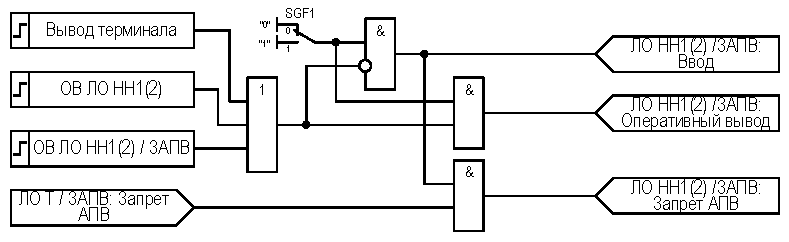
\includegraphics[width=0.9\textwidth,height=0.9\textheight,keepaspectratio]{img35.pdf}
\captionof{figure}{Функциональная схема <<Запрет АПВ>>}\label{lonn:img2}
\end{figure}

\small
\begin{longtable}{|>{\centering\arraybackslash}m{5.3cm}|>{\centering\arraybackslash}m{3.3cm}|>{\centering\arraybackslash}m{4.2cm}|>{\centering\arraybackslash}m{1.8cm}|>{\centering\arraybackslash}m{1cm}|}
\caption{Параметры для настройки функции <<Запрет АПВ>>\hfill\vspace{-0.5\baselineskip}}\label{lonn:tbl2}\\ 
\hline
\rowcolor{gray!30}
Параметр (Параметр на ИЧМ) & Условное обозначение на схеме & Значение/ Диапазон & Единица измерения & Шаг \\ 
\hline
\endfirsthead
\caption*{\hspace{3pt}\emph{Продолжение таблицы \ref{lonn:tbl2}\hfill\vspace{-0.5\baselineskip}}} \\ % сделано по ГОСТ 2.105 п.6.8.7
\hline
\rowcolor{gray!30}
Параметр (Параметр на ИЧМ) & Условное обозначение на схеме & Значение/ Диапазон & Единица измерения & Шаг \\ 
\endhead
\endfoot
\endlastfoot
\centering Ввод функции в работу (Ввод\_функции) & \centering SGF1 & \centering 0 = Не предусмотрено\\1 = Предусмотрено & \centering -- & \centering \arraybackslash -- \\
\hline
\end{longtable}
\normalsize

\end{enumerate}

\end{enumerate}
\FloatBarrier % Все float'ы ДО этой строки будут размещены здесь.
\needspace{4\baselineskip}
\color{uniblue}{\subsection{Устройство резервирования при отказе выключателя стороны ВН (УРОВ ВН)}}
\color{black}

\begin{enumerate}[label=\arabic{section}.\arabic{subsection}.\arabic*, labelsep=4pt, leftmargin=0pt, itemindent=57pt]

\item
Функция УРОВ предназначена для ликвидации повреждений, сопровождающихся отказом выключателя стороны ВН трансформатора.

\item
Основные характеристики функционального блока <<УРОВ ВН>>:
\begin{itemize}
    \item время срабатывания ИО тока при повышении тока скачком от 0 до $2I_{\textsl{уст.}}$ не более 30 мс;
    \item время возврата ИО тока при снижении тока скачком от $25I_{\textsl{ном}}$ до 0 не более 25 мс.
\end{itemize}

\item\label{urov:punkt}
В случае присутствия сигналов срабатывания защит от логики отключения стороны ВН трансформатора при введенном состоянии функция <<УРОВ ВН>>: 
\begin{itemize}
	\item формирует сигнал <<УРОВ: Пуск>> в следующих случаях:
		\begin{itemize}
		\sloppy
		\item если программный переключатель SGF2 <<Подхват\_по\_току>> находится в состоянии <<Не предусмотрено>> и через выключатель протекает ток, превышающий заданную уставку срабатывания ИО максимального тока функции <<УРОВ>> (в этом случае при пропадании сигнала пуска от защит возврат <<УРОВ>> может произойти раньше, чем наберется выдержка времени таймера T1 (уставка <<Тср>>), хотя ток через выключатель продолжает протекать); 
		\item если программный переключатель SGF2 <<Подхват\_по\_току>> находится в состоянии <<Предусмотрено>> и через выключатель протекает ток, превышающий заданную уставку срабатывания ИО максимального тока функции <<УРОВ>> (в этом случае сигнал пуска от защит запоминается на триггере, который сбрасывается по факту пропадания тока через выключатель);
		\end{itemize}
	\item формирует сигнал <<УРОВ: Срабатывание>> через выдержку таймера Т1 (уставка <<Тср>>) после появления сигнала <<УРОВ: Пуск>>.

\end{itemize}
\item
В случае присутствия сигналов срабатывания от внешних защит сторон НН трансформатора (активация сигнала <<Пуск УРОВ внешний>>) при введенном состоянии функция <<УРОВ ВН>>: 
\begin{itemize}
	\item формирует сигнал <<УРОВ: Сраб <<на себя>> для действия на отключение своего выключателя, при этом, в качестве дополнительного условия, есть возможность контроля протекания тока через выключатель от своих измерительных органов (программный переключатель SGF4 <<Контр\_тока\_на\_себя>> должен находиться в состоянии <<Предусмотрено>>);
	\item при введенном программном переключателе SGF3 <<Действ\_на\_выш\_выкл>> формирует сигналы <<УРОВ: Пуск>> и <<УРОВ: Срабатывание>> в случаях, описанных в пункте \ref{urov:punkt}.
\end{itemize}

\item
Ввод функции в работу на этапе параметрирования устройства осуществляется программным переключателем SGF1 <<Ввод\_функции>>. Информация о введенной функции отображается выходным сигналом <<УРОВ: Ввод>>.
\item
Функция <<УРОВ ВН>> может быть выведена из работы оперативно путем активации сигнала <<ОВ УРОВ ВН>>, что характеризуется активным состоянием сигнала <<УРОВ: Оперативный вывод>> на выходе функции.

\item
Алгоритм работы <<УРОВ>> выполнен в соответствии с рисунком \ref{urov35:img1}. В таблице \ref{urov35:tbl1} приведены параметры, необходимые для настройки функции <<УРОВ>>.

\vspace{3mm}
\begin{figure}[!h]
\centering
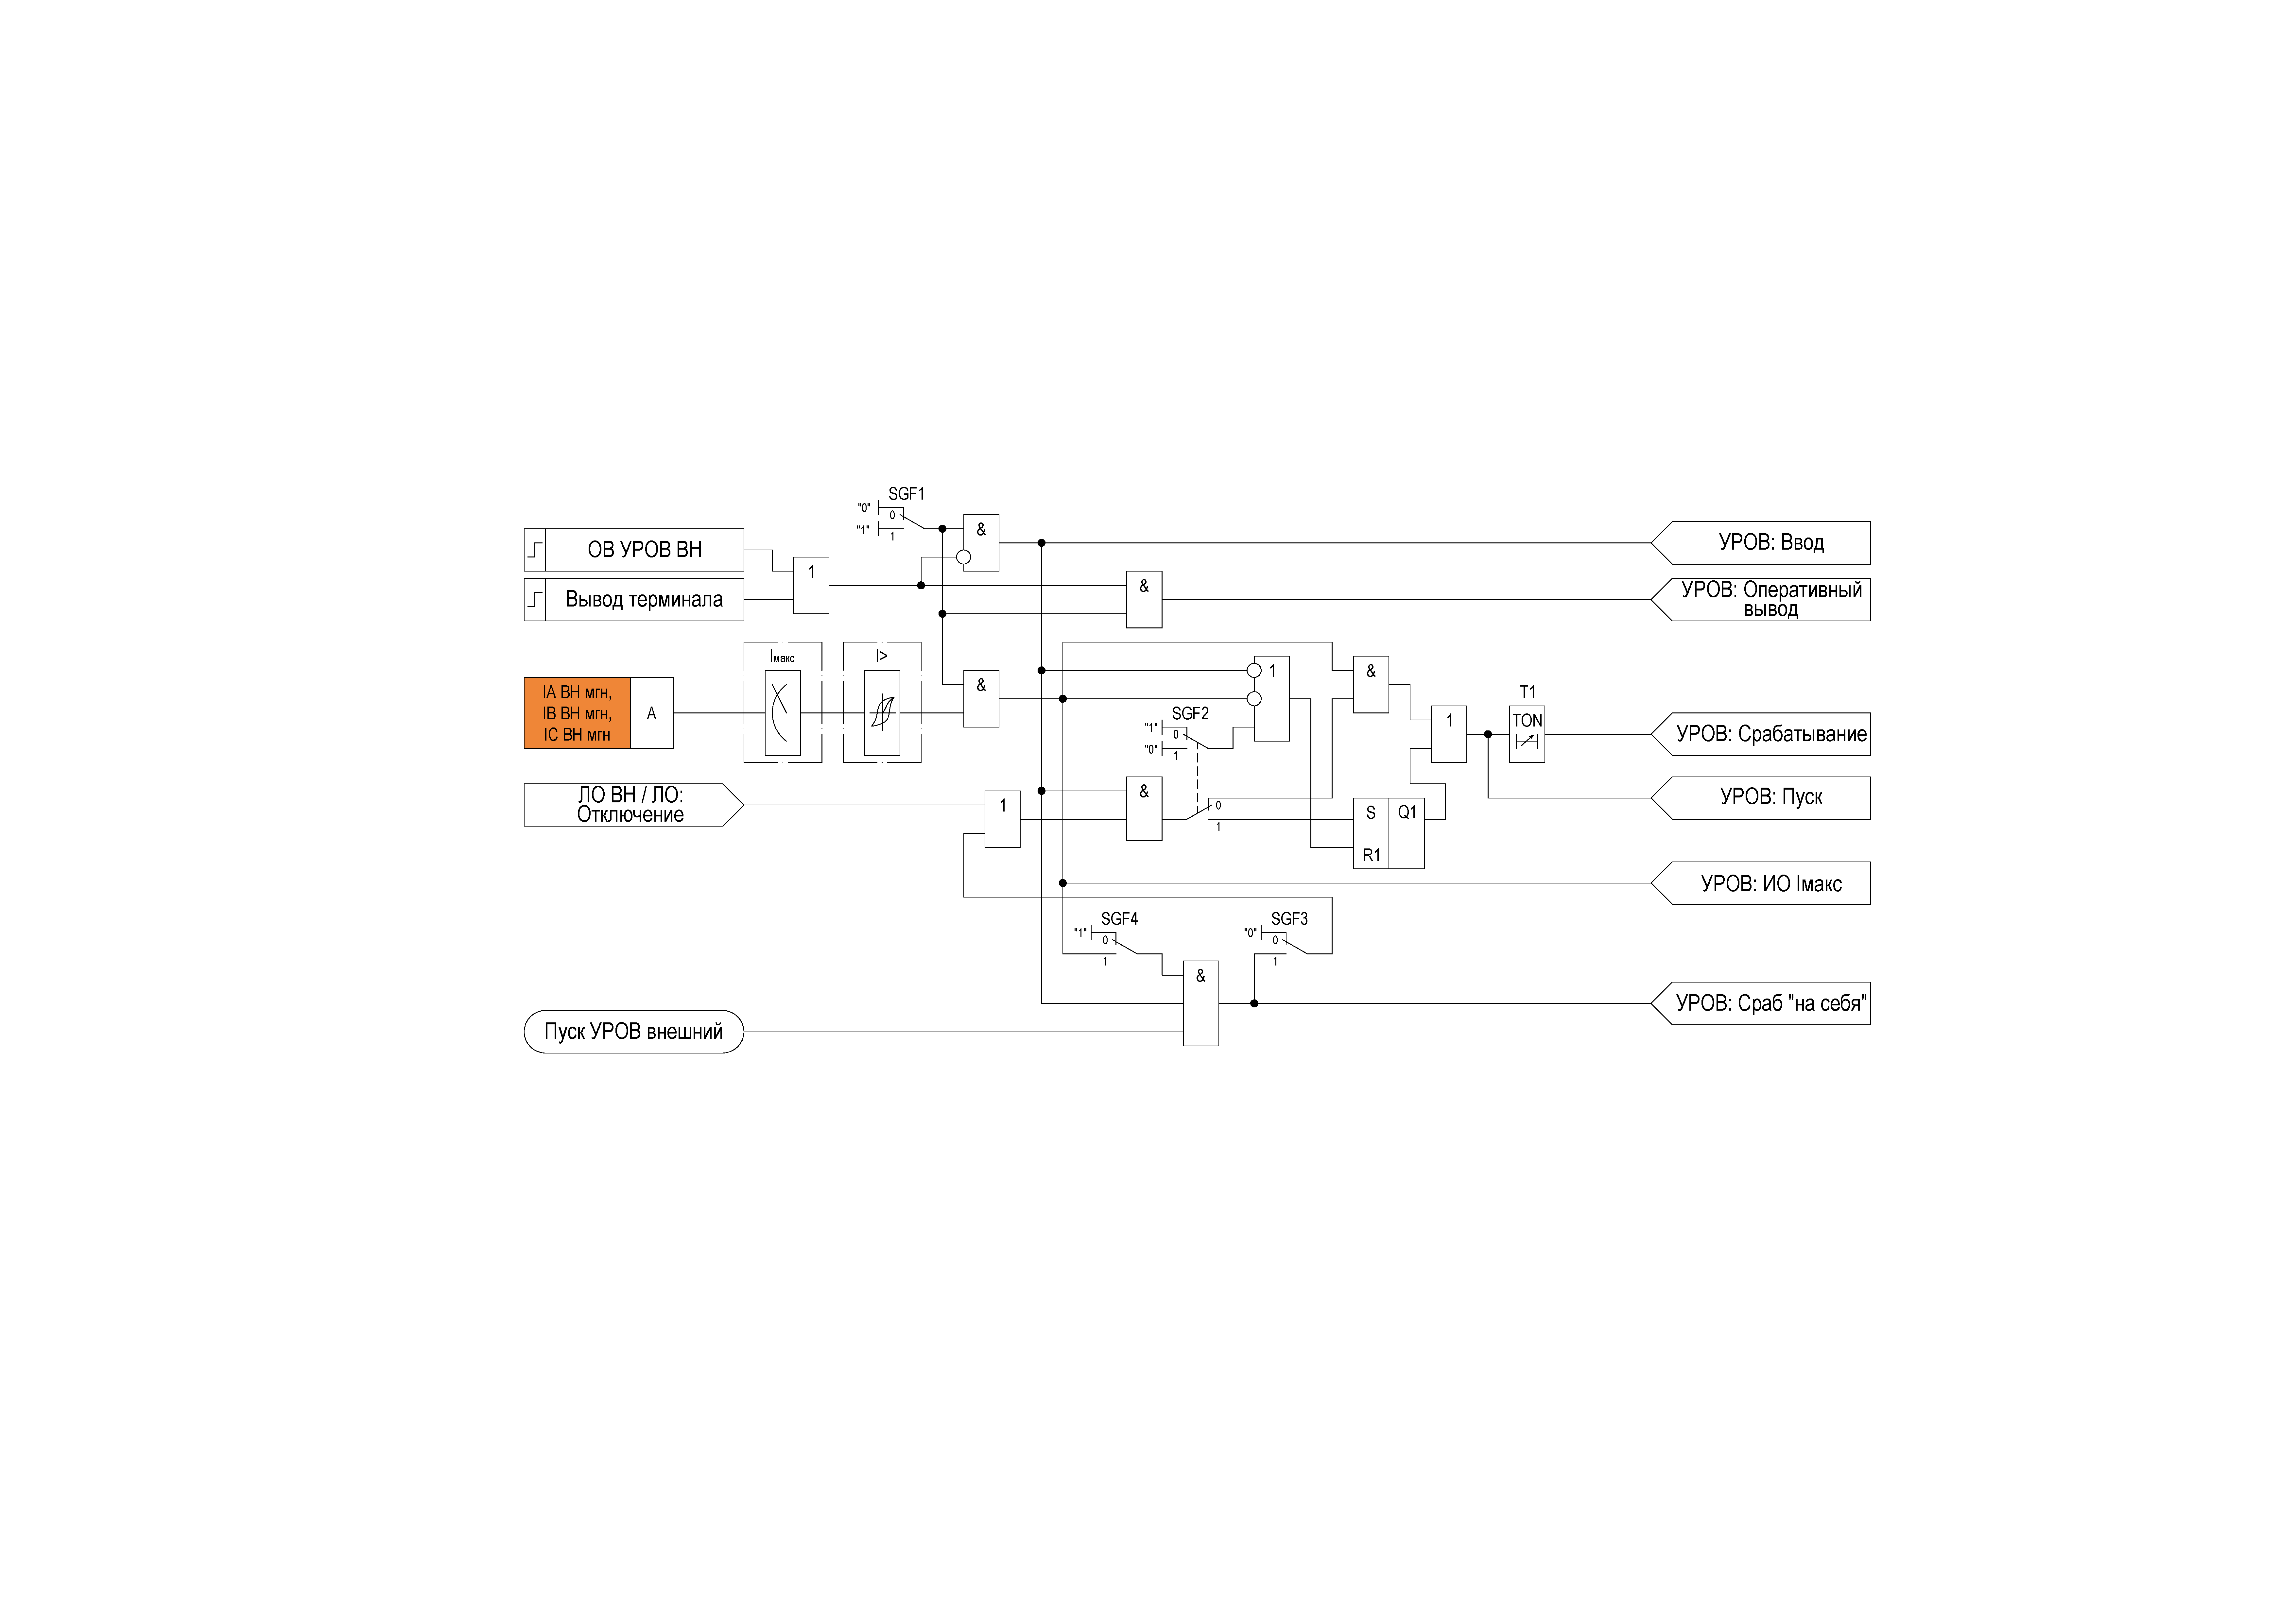
\includegraphics[width=\textwidth,height=\textheight,keepaspectratio]{img36.pdf}
\captionof{figure}{Функциональная схема <<УРОВ>>}\label{urov35:img1}
\end{figure}

\small
\begin{longtable}{|>{\centering\arraybackslash}m{5.3cm}|>{\centering\arraybackslash}m{3.3cm}|>{\centering\arraybackslash}m{4.2cm}|>{\centering\arraybackslash}m{1.8cm}|>{\centering\arraybackslash}m{1cm}|}
\caption{Параметры для настройки функции <<УРОВ>>\hfill\vspace{-0.5\baselineskip}}\label{urov35:tbl1}\\ 
\hline
\rowcolor{gray!30}
Параметр (Параметр на ИЧМ) & Условное обозначение на схеме & Значение/ Диапазон & Единица измерения & Шаг \\ 
\hline
\endfirsthead
\caption{\emph{Продолжение\hfill\vspace{-0.5\baselineskip}}} \\ % Отступ обозначения таблицы от таблицы и выравнивание надписи слева
\hline
\rowcolor{gray!30}
Параметр (Параметр на ИЧМ) & Условное обозначение на схеме & Значение/ Диапазон & Единица измерения & Шаг \\ 
\endhead
\endfoot
\endlastfoot
\centering Ввод функции в работу (Ввод\_функции) & \centering SGF1 & \centering 0 = Не предусмотрено\\1 = Предусмотрено & \centering -- & \centering \arraybackslash -- \\
\hline
\centering Ток срабатывания (Iср) & \centering I$>$ & \centering 0,05 ... 0,50 & \centering о.е. & \centering \arraybackslash 0,01 \\
\hline
\centering УРОВ с подхватом по току (Подхват\_по\_току) & \centering SGF2 & \centering 0 = Не предусмотрено\\1 = Предусмотрено & \centering -- & \centering \arraybackslash -- \\
\hline
\centering Контроль по току при действии «на себя» (Контр\_тока\_на\_себя) & \centering SGF4 & \centering 0 = Не предусмотрено\\1 = Предусмотрено & \centering -- & \centering \arraybackslash -- \\
\hline
\centering Выдержка времени срабатывания (Tср) & \centering T1 & \centering 0,00 ... 1,00 & \centering с & \centering \arraybackslash 0,01 \\
\hline
\centering Действие внешнего УРОВ на вышестоящий выключатель (Действ\_на\_выш\_выкл) & \centering SGF3 & \centering 0 = Не предусмотрено\\1 = Предусмотрено & \centering -- & \centering \arraybackslash -- \\
\hline
\end{longtable}
\normalsize

\end{enumerate}
\FloatBarrier % Все float'ы ДО этой строки будут размещены здесь.


\needspace{4\baselineskip}
\color{uniblue}{\subsection{Сборка сигналов (СС)}}
\color{black}

\begin{enumerate}[label=\arabic{section}.\arabic{subsection}.\arabic*, labelsep=4pt, leftmargin=0pt, itemindent=57pt]

\item
Функциональный блок <<СС>> используется в качестве дополнительной логики для предупредительной сигнализации, которая описана в подразделе \ref{ps:punkt}.
\item
Функция <<СС>>  принимает различные сигналы от других функций и формирует следующие обобщенные сигналы:
\begin{itemize}
	\item общий сигнал срабатывания реле газовых защит <<СС: ГЗ сигн>>;
	\item общий сигнал неисправности изоляции цепей газовых защит <<СС: Низ.изол. ГЗ>>;
	\item общий сигнал блокировки цепей газовых защит <<СС: ГЗ заблокирована>>;
	\item общий сигнал срабатывания датчиков технологических защит <<СС: ТЗ сигн>>;
	\item общий сигнал неисправности изоляции цепей технологических защит <<СС: Низ.изол. ТЗ>>;
	\item общий сигнал блокировки цепей технологических защит <<СС: ТЗ заблокирована>>;	
	\item общий сигнал срабатывания датчиков технологической сигнализации <<СС: ТС сигн>>;
	\item общий сигнал неисправности оперативного тока газовых и технологических защит <<СС: ОТ сигн>>;	
	\item общий сигнал неисправности оперативного тока дуговых защит и УРОВ стороны НН <<СС: ОТ НН сигн>>;
	\item общий сигнал срабатывания дуговых защит и УРОВ стороны НН <<СС: Внеш. откл>>;
	\item сигнал нарушения положения переключателей в выходных цепях  <<СС: Вых.цепи разобраны>>;
	\item сигнал нарушения положения испытательных блоков <<СС:БИ выведены>>;
	\item общий сигнал срабатывания внешних функций <<СС:Общ. внеш. сигнал>>.	
\end{itemize}

\item
Выходные сигналы функционального блока могут быть использованы для дальнейшего конфигурирования (например, на выходные реле) и применяться в цепях участковых и индивидуальных табло, сигнальных ламп, сигнальных реле, звуковой сигнализации и пр.

\item
Логика работы функционального блока <<СС>> выполнена в соответствии с рисунком \ref{ss:img1}. В таблице \ref{ss:tbl1} приведены параметры, необходимые для настройки функционального блока <<СС>>. 

\small
\begin{longtable}{|>{\centering\arraybackslash}m{5.3cm}|>{\centering\arraybackslash}m{3.3cm}|>{\centering\arraybackslash}m{4.2cm}|>{\centering\arraybackslash}m{1.8cm}|>{\centering\arraybackslash}m{1cm}|}
\caption{Параметры для настройки функции <<СС>>\hfill\vspace{-0.5\baselineskip}}\label{ss:tbl1}\\ 
\hline
\rowcolor{gray!30}
Параметр (Параметр на ИЧМ) & Условное обозначение на схеме & Значение/ Диапазон & Единица измерения & Шаг \\ 
\hline
\endfirsthead
\caption*{\hspace{3pt}\emph{Продолжение таблицы \ref{ss:tbl1}\hfill\vspace{-0.5\baselineskip}}} \\ % сделано по ГОСТ 2.105 п.6.8.7
\hline
\rowcolor{gray!30}
Параметр (Параметр на ИЧМ) & Условное обозначение на схеме & Значение/ Диапазон & Единица измерения & Шаг \\ 
\endhead
\endfoot
\endlastfoot
\centering Контроль положения SA1 (Контр\_полож\_SA1) & \centering SGF1 & \centering 0 = Не предусмотрено\\1 = Предусмотрено & \centering -- & \centering \arraybackslash -- \\
\hline
\centering Контроль положения SA2 (Контр\_полож\_SA2) & \centering SGF2 & \centering 0 = Не предусмотрено\\1 = Предусмотрено & \centering -- & \centering \arraybackslash -- \\
\hline
\centering Контроль положения SA3 (Контр\_полож\_SA3) & \centering SGF3 & \centering 0 = Не предусмотрено\\1 = Предусмотрено & \centering -- & \centering \arraybackslash -- \\
\hline
\centering Контроль положения SA4 (Контр\_полож\_SA4) & \centering SGF4 & \centering 0 = Не предусмотрено\\1 = Предусмотрено & \centering -- & \centering \arraybackslash -- \\
\hline
\centering Контроль положения SG1 (Контр\_полож\_SG1) & \centering SGF5 & \centering 0 = Не предусмотрено\\1 = Предусмотрено & \centering -- & \centering \arraybackslash -- \\
\hline
\centering Контроль положения SG2 (Контр\_полож\_SG2) & \centering SGF6 & \centering 0 = Не предусмотрено\\1 = Предусмотрено & \centering -- & \centering \arraybackslash -- \\
\hline
\centering Контроль положения SG3 (Контр\_полож\_SG3) & \centering SGF7 & \centering 0 = Не предусмотрено\\1 = Предусмотрено & \centering -- & \centering \arraybackslash -- \\
\hline
\centering Контроль опер. тока цепей ГЗ (Контр\_ОТ\_ГЗ) & \centering SGF8 & \centering 0 = Не предусмотрено\\1 = Предусмотрено & \centering -- & \centering \arraybackslash -- \\
\hline
\centering Контроль опер. тока цепей ТЗ, ТС (Контр\_ОТ\_ТЗ\_ТС) & \centering SGF9 & \centering 0 = Не предусмотрено\\1 = Предусмотрено & \centering -- & \centering \arraybackslash -- \\
\hline
\centering Контроль опер. тока цепей ЗДЗ НН1 (Контр\_ОТ\_ЗДЗ1) & \centering SGF10 & \centering 0 = Не предусмотрено\\1 = Предусмотрено & \centering -- & \centering \arraybackslash -- \\
\hline
\centering Контроль опер. тока цепей ЗДЗ НН2 (Контр\_ОТ\_ЗДЗ2) & \centering SGF11 & \centering 0 = Не предусмотрено\\1 = Предусмотрено & \centering -- & \centering \arraybackslash -- \\
\hline
\centering Контроль опер. тока цепей УРОВ НН1 (Контр\_ОТ\_УРОВ1) & \centering SGF12 & \centering 0 = Не предусмотрено\\1 = Предусмотрено & \centering -- & \centering \arraybackslash -- \\
\hline
\centering Контроль опер. тока цепей УРОВ НН2 (Контр\_ОТ\_УРОВ2) & \centering SGF13 & \centering 0 = Не предусмотрено\\1 = Предусмотрено & \centering -- & \centering \arraybackslash -- \\
\hline
\end{longtable}
\normalsize

\vspace{2mm}
\begin{figure}[!h]
\centering
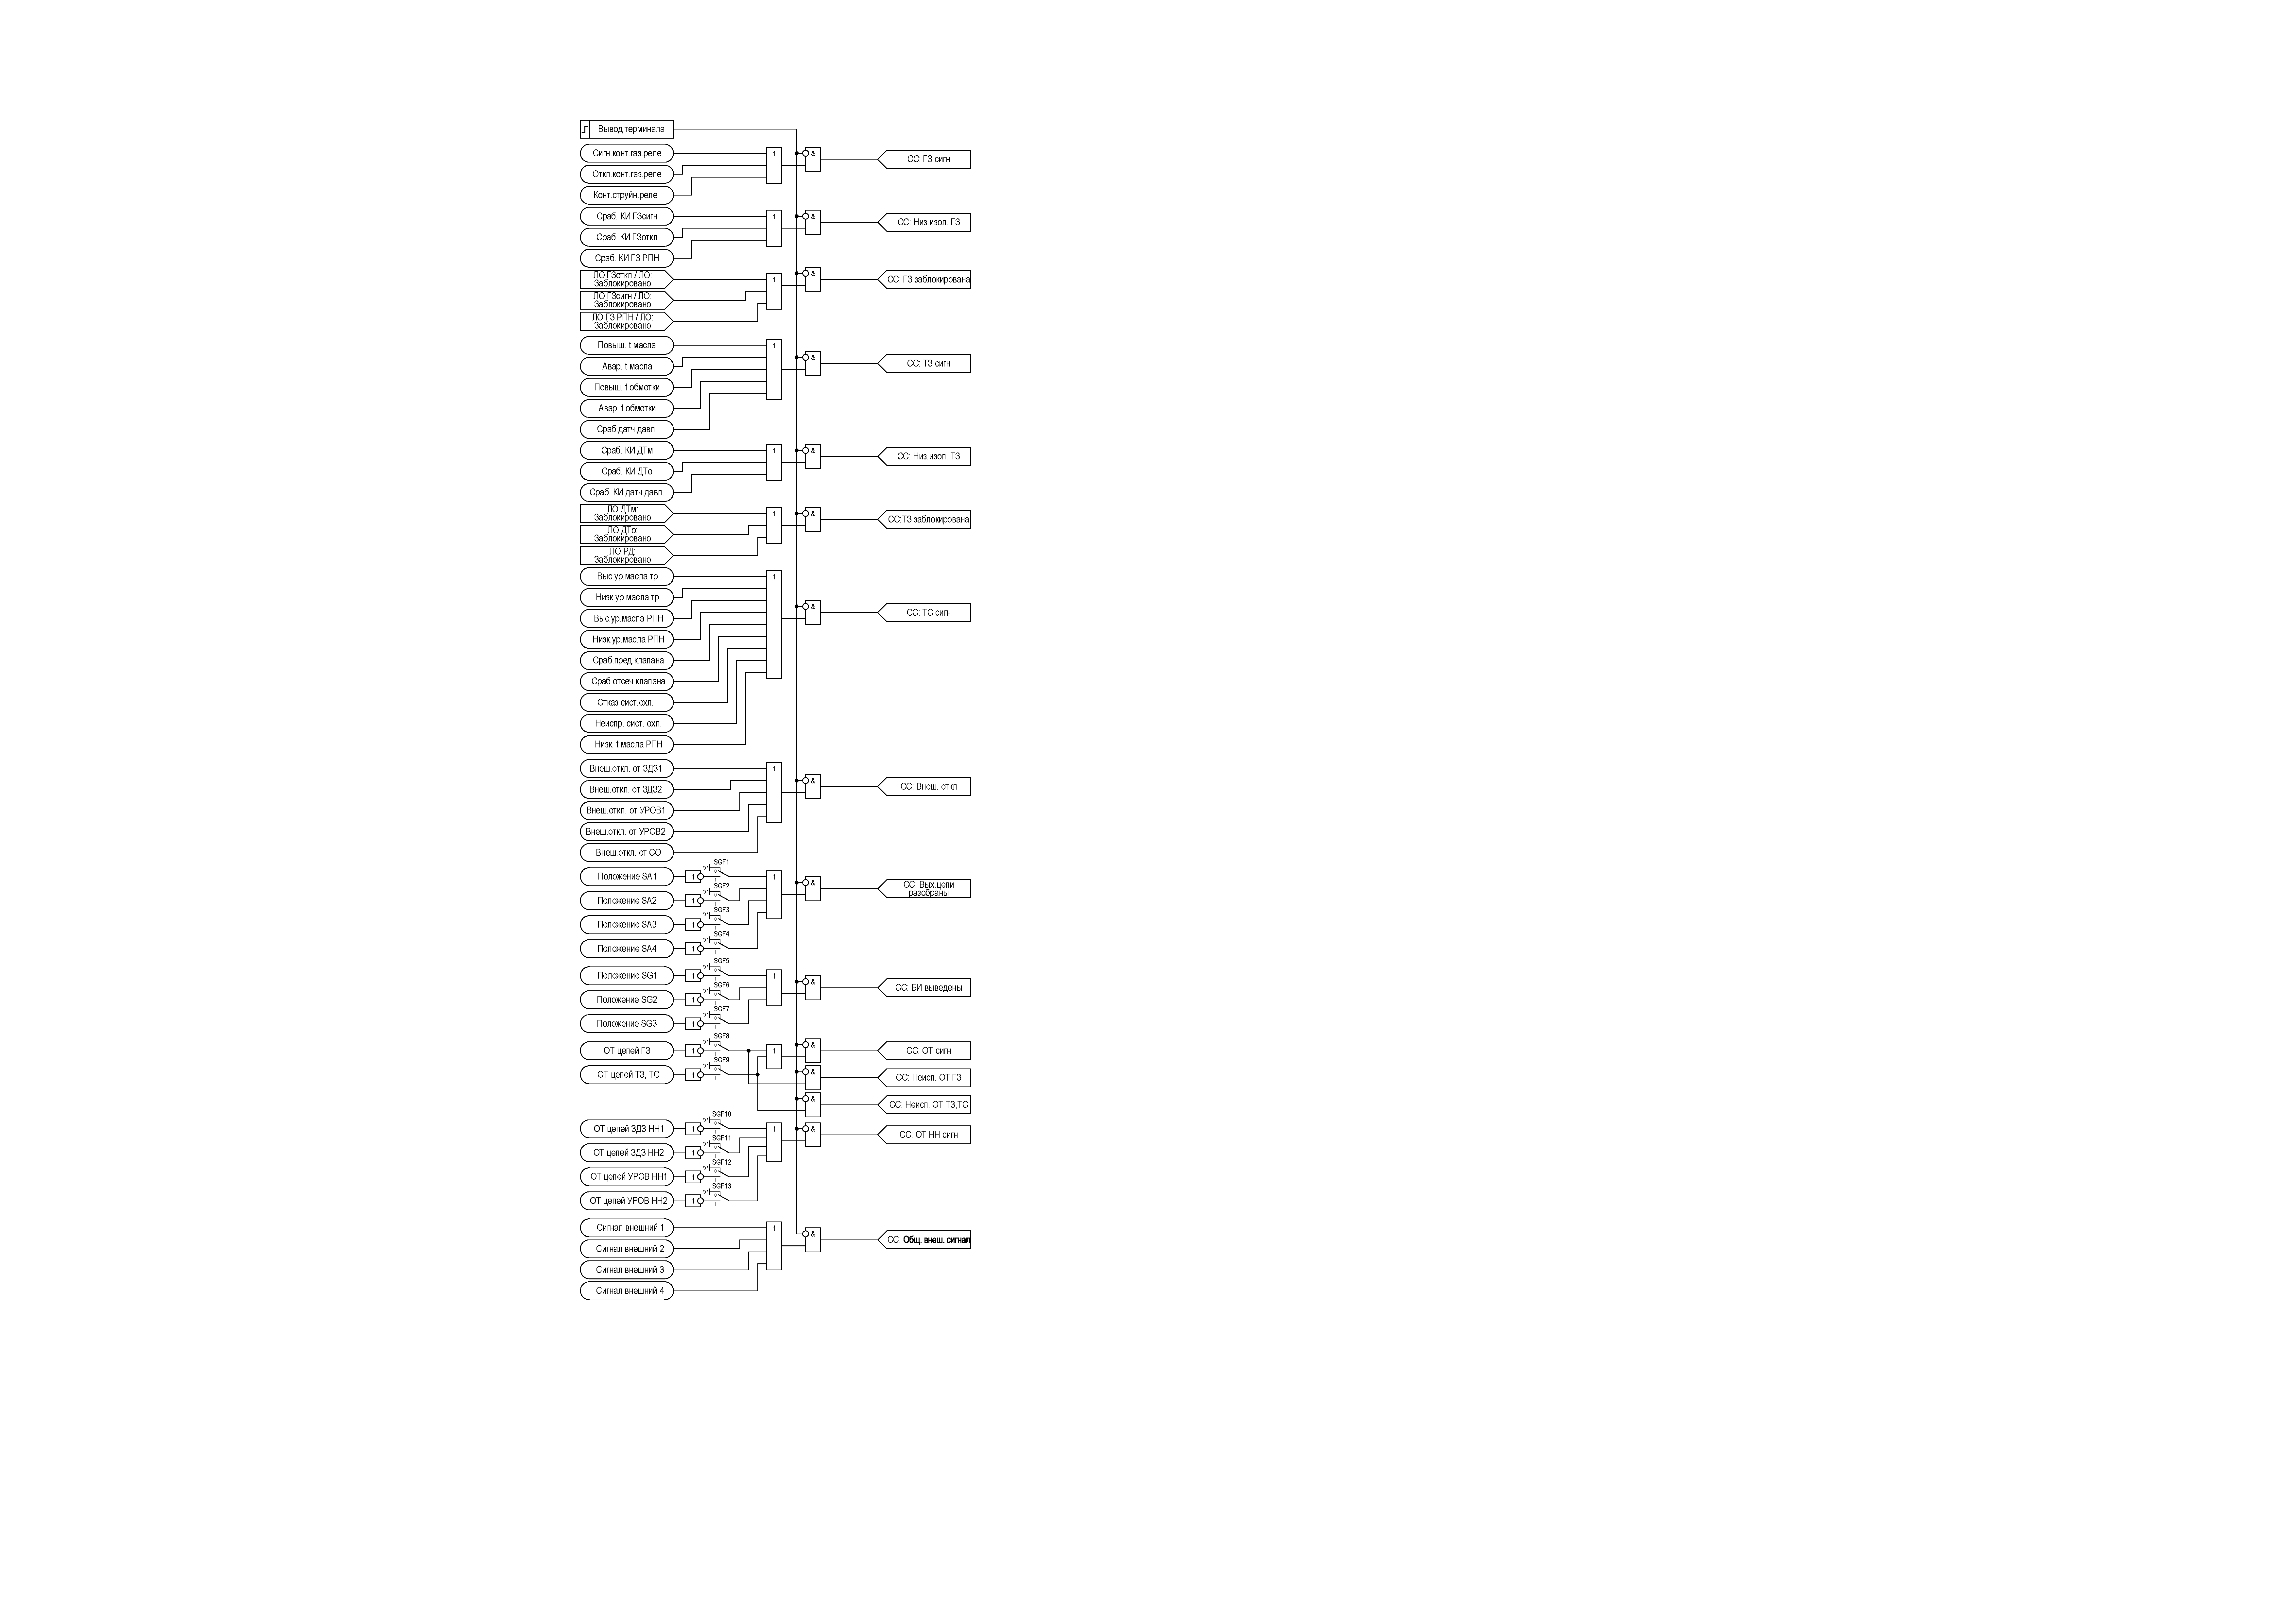
\includegraphics[width=0.95\textwidth,height=0.95\textheight,keepaspectratio]{img37.pdf}
\captionof{figure}{Функциональная схема <<СС>>}\label{ss:img1}
\end{figure}

\end{enumerate}
\FloatBarrier % Все float'ы ДО этой строки будут размещены здесь.
\needspace{4\baselineskip}
\color{uniblue}{\subsection{Предупредительная сигнализация устройства (ПС)\label{ps:punkt}}}
\color{black}

\begin{enumerate}[label=\arabic{section}.\arabic{subsection}.\arabic*, labelsep=4pt, leftmargin=0pt, itemindent=57pt]

\item	
Предупредительная сигнализация предназначена для информирования оперативного персонала при отклонениях от нормального режима работы оборудования энергообъекта.

\item
Функциональный блок <<ПС>> принимает сигналы срабатывания защитных и сервисных функций устройства и формирует следующие сигналы:
\begin{itemize}
	\item импульсный сигнал предупредительной сигнализации <<ПС: Пуск (имп)>>;
	\item длительный сигнал предупредительной сигнализации <<ПС: Пуск>>.
\end{itemize}

\item
Выходные сигналы функционального блока могут быть использованы для дальнейшего конфигурирования (например, на выходные реле) и применяться в цепях участковых и индивидуальных табло, сигнальных ламп, сигнальных реле, звуковой сигнализации и пр.
\item
Логика работы <<ПС>> выполнена в соответствии с рисунком \ref{ps:img1}. В таблице \ref{ps:tbl1} приведены параметры, необходимые для настройки функционального блока <<ПС>>. 

\small
\begin{longtable}{|>{\centering\arraybackslash}m{5.3cm}|>{\centering\arraybackslash}m{3.3cm}|>{\centering\arraybackslash}m{4.2cm}|>{\centering\arraybackslash}m{1.8cm}|>{\centering\arraybackslash}m{1cm}|}
\caption{Параметры для настройки функции <<ПС>>\hfill\vspace{-0.5\baselineskip}}\label{ps:tbl1}\\ 
\hline
\rowcolor{gray!30}
Параметр (Параметр на ИЧМ) & Условное обозначение на схеме & Значение/ Диапазон & Единица измерения & Шаг \\ 
\hline
\endfirsthead
\caption*{\hspace{3pt}\emph{Продолжение таблицы \ref{ps:tbl1}\hfill\vspace{-0.5\baselineskip}}} \\ % сделано по ГОСТ 2.105 п.6.8.7
\hline
\rowcolor{gray!30}
Параметр (Параметр на ИЧМ) & Условное обозначение на схеме & Значение/ Диапазон & Единица измерения & Шаг \\ 
\endhead
\endfoot
\endlastfoot
\centering Контроль сигнала «ГЗ сигн» (Контр\_ГЗ\_сигн) & \centering SGF1 & \centering 0 = Не предусмотрено\\1 = Предусмотрено & \centering -- & \centering \arraybackslash -- \\
\hline
\centering Контроль сигнала «Низ. изол. ГЗ» (Контр\_Низ\_изол\_ГЗ) & \centering SGF2 & \centering 0 = Не предусмотрено\\1 = Предусмотрено & \centering -- & \centering \arraybackslash -- \\
\hline
\centering Контроль сигнала «ГЗ заблокирована» (Контр\_ГЗ\_блок) & \centering SGF3 & \centering 0 = Не предусмотрено\\1 = Предусмотрено & \centering -- & \centering \arraybackslash -- \\
\hline
\centering Контроль сигнала «ТЗ сигн» (Контр\_ТЗ\_сигн) & \centering SGF4 & \centering 0 = Не предусмотрено\\1 = Предусмотрено & \centering -- & \centering \arraybackslash -- \\
\hline
\centering Контроль сигнала «Низ. изол. ТЗ» (Контр\_Низ\_изол\_ТЗ) & \centering SGF5 & \centering 0 = Не предусмотрено\\1 = Предусмотрено & \centering -- & \centering \arraybackslash -- \\
\hline
\centering Контроль сигнала «ТЗ заблокирована» (Контр\_ТЗ\_блок) & \centering SGF6 & \centering 0 = Не предусмотрено\\1 = Предусмотрено & \centering -- & \centering \arraybackslash -- \\
\hline
\centering Контроль сигнала «ТС сигн» (Контр\_ТС\_сигн) & \centering SGF7 & \centering 0 = Не предусмотрено\\1 = Предусмотрено & \centering -- & \centering \arraybackslash -- \\
\hline
\centering Контроль сигнала «ОТ сигн» (Контр\_ОТ\_сигн) & \centering SGF8 & \centering 0 = Не предусмотрено\\1 = Предусмотрено & \centering -- & \centering \arraybackslash -- \\
\hline
\centering Контроль сигнала «ОТ НН сигн» (Контр\_ОТ\_НН\_сигн) & \centering SGF9 & \centering 0 = Не предусмотрено\\1 = Предусмотрено & \centering -- & \centering \arraybackslash -- \\
\hline
\centering Контроль сигнала «Внеш. откл» (Контр\_Внеш\_откл) & \centering SGF10 & \centering 0 = Не предусмотрено\\1 = Предусмотрено & \centering -- & \centering \arraybackslash -- \\
\hline
\centering Контроль сигнала «Вых. цепи разобраны» (Контр\_Вых\_цеп\_разоб) & \centering SGF11 & \centering 0 = Не предусмотрено\\1 = Предусмотрено & \centering -- & \centering \arraybackslash -- \\
\hline
\centering Контроль сигнала «БИ выведены» (Контр\_БИ\_выведены) & \centering SGF12 & \centering 0 = Не предусмотрено\\1 = Предусмотрено & \centering -- & \centering \arraybackslash -- \\
\hline
\centering Контроль общего внешнего сигнала (Контр\_общ\_внеш\_сигн) & \centering SGF13 & \centering 0 = Не предусмотрено\\1 = Предусмотрено & \centering -- & \centering \arraybackslash -- \\
\hline
\end{longtable}
\normalsize

\begin{figure}[!h]
\centering
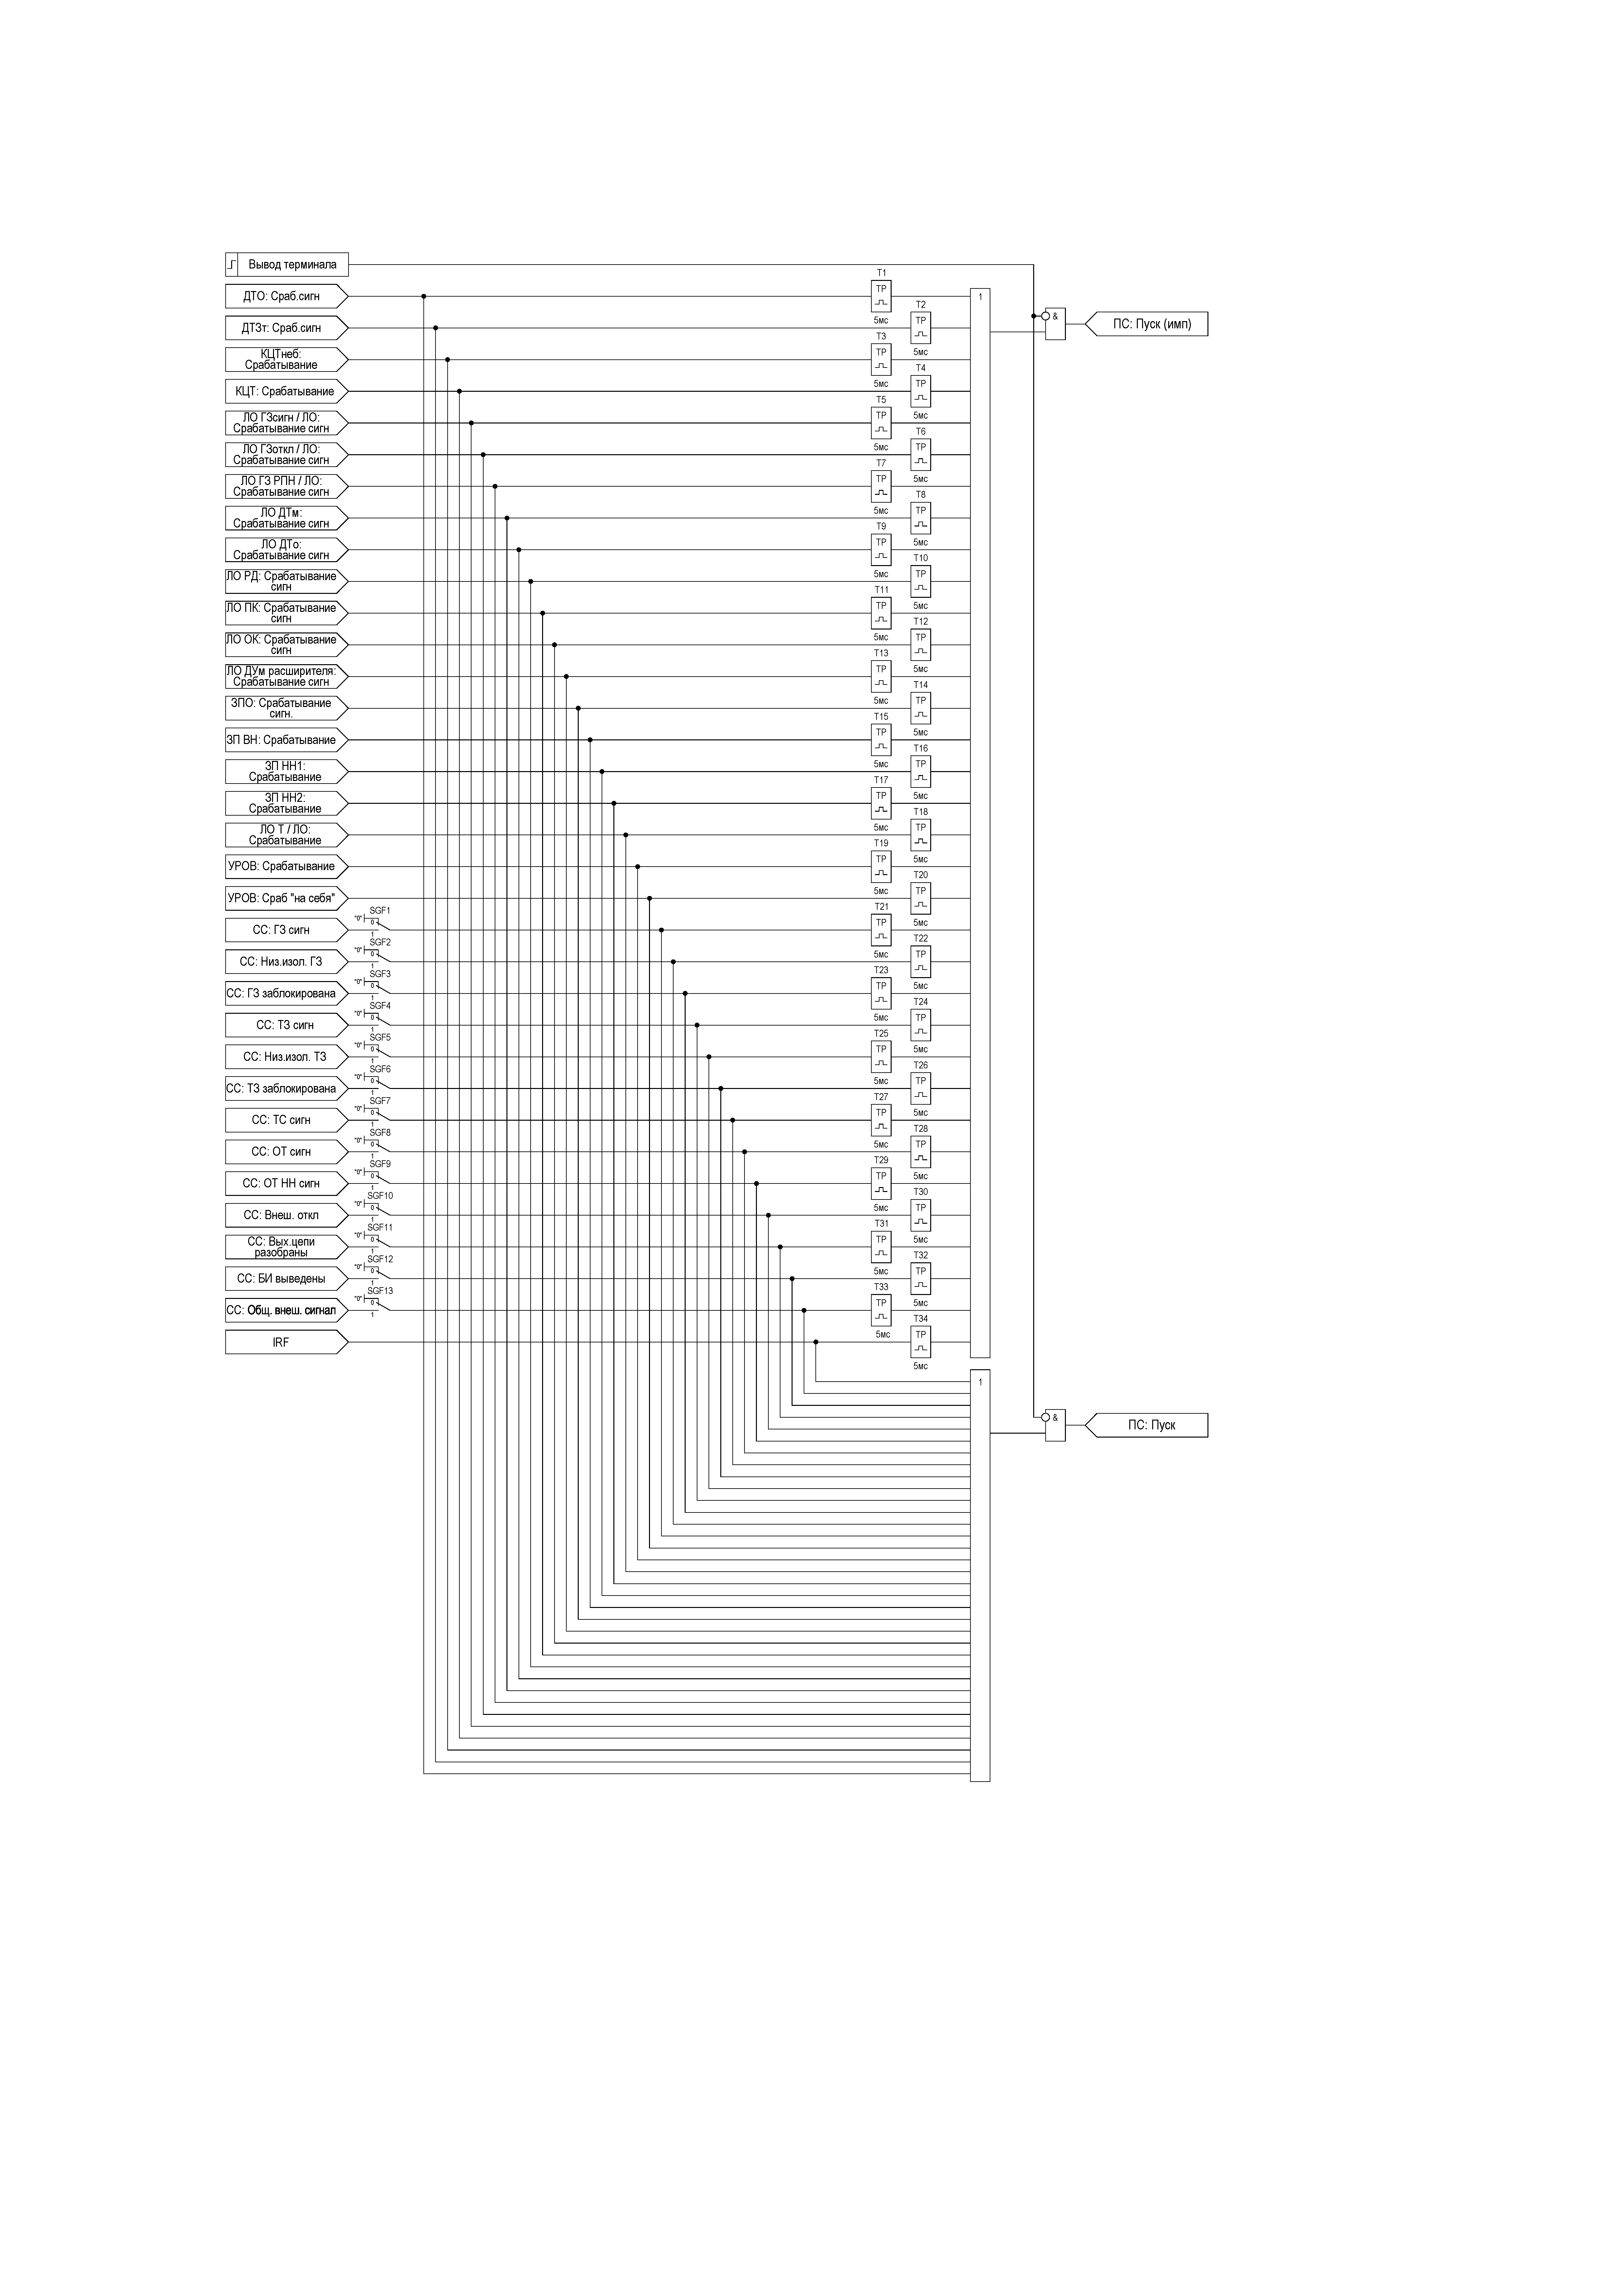
\includegraphics[width=0.95\textwidth,height=0.95\textheight,keepaspectratio]{img38.pdf}
\captionof{figure}{Функциональная схема <<ПС>>}\label{ps:img1}
\end{figure}

\end{enumerate}
\FloatBarrier % Все float'ы ДО этой строки будут размещены здесь.
\newpage
\color{uniblue}\section[Использование по назначению]{Использование по назначению}\label{sec:using}
\color{black}

\color{uniblue}\subsection{Эксплуатационные ограничения}\color{black}
Климатические условия эксплуатации должны соответствовать требованиям документа ЮТКБ.656122.609 РЭ <<Устройство защиты и автоматики серии <<ЮНИТ-М300>>. Руководство по эксплуатации общее>>.

\color{uniblue}\subsection{Подготовка устройства к использованию}\color{black}
Меры безопасности при подготовке устройства, порядок проведения внешнего осмотра устройства перед использованием, требования к монтажу устройства, подключение к персональному компьютеру и устройству <<ЮНИТ-ИЧМ>> приводится в документации ЮТКБ.656122.609 РЭ <<Устройство защиты и автоматики серии <<ЮНИТ-М300>>. Руководство по эксплуатации общее>>.

\color{uniblue}\subsection{Работа с устройством}\color{black}

\begin{enumerate}[label=\arabic{section}.\arabic{subsection}.\arabic*, labelsep=4pt, leftmargin=0pt, itemindent=57pt]
    \item
    Взаимодействие с устройством осуществляется при помощи подключаемого устройства <<ЮНИТ-ИЧМ>> или через персональный компьютер с установленным программным обеспечением <<ЮНИТ-СЕРВИС>>. Руководство по устройству <<ЮНИТ-ИЧМ>> представлено в документе ЮТКБ.656132.701 РЭ <<Блок интерфейсный <<ЮНИТ-ИЧМ>>. Руководство по эксплуатации>>. Руководство по использованию программного обеспечения представлено в документе RU.37182817.00001.02.34.01 <<Программное обеспечение мониторинга и параметрирования <<ЮНИТ-СЕРВИС>>. Руководство пользователя>>.
    
    
    \end{enumerate}
    
    \par
    Описание работы с устройством (включение, способы управления устройством, обновление встроенного программного обеспечения, неисправности и методы их устранения) приводится в документации ЮТКБ.656122.609 РЭ <<Устройство защиты и автоматики серии <<ЮНИТ-М300>>. Руководство по эксплуатации общее>>.\newpage
\color{uniblue}\section[Техническое обслуживание и ремонт]{Техническое обслуживание и ремонт}\label{sec:techrepair}
\color{black}

\color{uniblue}\subsection{Техническое обслуживание устройства}\color{black}

\begin{enumerate}[label=\arabic{section}.\arabic{subsection}.\arabic*, labelsep=4pt, leftmargin=0pt, itemindent=57pt]

\item\sloppy
Процесс  технического  обслуживания  устройств  релейной  защиты  регламентирован  приказом Минэнерго  России  «Об  утверждении  Правил  технического  обслуживания  устройств  и  комплексов релейной  защиты  и  автоматики  и  внесении  изменений  в  требования  к  обеспечению  надежности электроэнергетических  систем,  надежности  и  безопасности  объектов  электроэнергетики  и энергопринимающих установок».
\item
Техническое обслуживание устройств <<ЮНИТ-М300>> должно выполняться в соответствии с документом ЮТКБ.656122.609 ИС – <<Устройства защиты и автоматики серии <<ЮНИТ-М300>>. Инструкция эксплуатационная специальная. Методические указания по выполнению технического обслуживания>>.

\end{enumerate}

\color{uniblue}\subsection{Текущий ремонт}\color{black}

\begin{enumerate}[label=\arabic{section}.\arabic{subsection}.\arabic*, labelsep=4pt, leftmargin=0pt, itemindent=57pt]

\item
Устройство серии <<ЮНИТ-М300>>, как было описано выше, выполнено с использованием микропроцессорных технологий, поэтому необходимость в его текущем ремонте отсутствует. Работоспособность и безотказность работы устройства обеспечивается функционированием системы самодиагностики.
\item
Углубленная самодиагностика аппаратных средств, а также состояние программной памяти, памяти данных  и  буферной  памяти  производится  при  включении  устройства.  Поэтому  при  возникновении сообщений о критических или некритических ошибках от системы самодиагностики, даже при возможности устранения  их  своими  силами,  следует  обратиться  на  предприятие-изготовитель для  консультации или проведения регламентных работ.
\item 
Поводом  для  обращения  на  предприятие-изготовитель  являются  также  признаки  нехарактерного нагрева или перегрева отдельных элементов, участков или частей устройства.
\item
Вышедшие  из  строя  устройства  должны  проходить  ремонт  на  предприятии-изготовителе, обеспечивающем  гарантийное  и  послегарантийное  обслуживание, адрес которого  указан  в  паспорте устройства.  В  качестве  ЗИП,  если  это  предусмотрено  договором  поставки,  могут  предоставляться устройства  <<ЮНИТ-М300>> с необходимыми  конфигурациями,  позволяющие  оперативно  произвести  замену вышедших из строя устройств.
\item
Перечень сигналов самодиагностики приведен в документации ЮТКБ.656122.609 РЭ <<Устройство защиты и автоматики серии <<ЮНИТ-М300>>. Руководство по эксплуатации общее>>.
\end{enumerate}


\vspace{5mm}
\color{uniblue}\section[Транспортирование, хранение и консервация]{Транспортирование, хранение и консервация}\label{sec:trans}
\color{black}


Более подробно об условиях транспортирования и хранения устройства можно узнать в соответствующем разделе документации ЮТКБ.656122.609 РЭ <<Устройство защиты и автоматики серии <<ЮНИТ-М300>>. Руководство по эксплуатации общее>>. 

\vspace{3mm}
\color{uniblue}\section[Утилизация]{Утилизация}\label{sec:util}
\color{black}

\begin{enumerate}[label=\arabic{section}.\arabic*, labelsep=4pt, leftmargin=0pt, itemindent=57pt]

\item
Демонтаж и утилизация устройства не требуют применения специальных мер безопасности и выполняются без применения специальных приспособлений и инструментов.
\item
Более подробно о способах утилизации устройства можно узнать в соответствующем разделе документации ЮТКБ.656122.609 РЭ <<Устройство защиты и автоматики серии <<ЮНИТ-М300>>. Руководство по эксплуатации общее>>.

\end{enumerate}

\vspace{3mm}
\color{uniblue}\section[Гарантия изготовителя]{Гарантия изготовителя}\label{sec:garantee}
\color{black}

\begin{enumerate}[label=\arabic{section}.\arabic*, labelsep=4pt, leftmargin=0pt, itemindent=57pt]

\item
Гарантийный срок эксплуатации устройства составляет 36 месяцев со дня ввода устройства в эксплуатацию, но не более 40 месяцев с даты производства предприятием-изготовителем или с момента проследования через государственную границу при поставках на экспорт.
\item
Более подробно о гарантийных обязательствах изготовителя устройства можно узнать в соответствующем разделе документации ЮТКБ.656122.609 РЭ <<Устройство защиты и автоматики серии <<ЮНИТ-М300>>. Руководство по эксплуатации общее>>. 

\end{enumerate}\vspace{3mm}
\color{uniblue}\section[Техническая поддержка]{Техническая поддержка}\label{sec:support}
\color{black}

\noindent
Сервисный  центр  ООО  «Юнител  Инжиниринг»  принимает  заявки  от  потребителей  о  качестве функционирования  оборудования  и  ПО,  оказывает  консультационные  услуги  при  поиске  и  устранении неисправностей.
\par
\noindent
Заявки от потребителей принимаются  по  телефонной  связи  (тел.:  +7 (495) 165-99-98) и (или) по электронной почте:
\vskip 1mm

\href{mailto:rza@uni-eng.ru}{\color{uniblue}\uline{rza@uni-eng.ru}}
\vskip 1mm

\href{mailto:info@uni-eng.ru}{\color{uniblue}\uline{info@uni-eng.ru}}
\vskip 1mm

\noindent
Форму заявки можно скачать по ссылке: 

\href{https://uni-eng.ru/support/servisnyy-tsentr/}{\color{uniblue}\uline{https://uni-eng.ru/support/servisnyy-tsentr/}}.



\appendixtitleon
\appendixtitletocon

\settocdepth{section}

\makeatletter
\renewcommand{\Asbuk}[1]{\expandafter\@Asbuk\csname c@#1\endcsname}
\def\@Asbuk#1{\ifcase#1\or
 А\or Б\or В\or Г\or Д\or Е\or Ж\or И\or К\or Л\or М\or Н\or О\or П\or Р\or С\or Т\or У\or Ф\or Х\or Ц\or Ч\or Ш\or Щ\or Э\or Ю\or Я\else\@ctrerr\fi}
\makeatother

\begin{appendices}

\renewcommand{\thesection}{\Asbuk{section}}

\titleformat{\section}[display]
  {\normalfont\large\bfseries}
  {\centering Приложение\ \thesection}
  {0pt}{\large\centering}




\newpage
\newgeometry{
  top=14mm,
  bottom=11mm,
  right=10mm,
  left=22mm,
}

\begin{landscape}

\setlength{\footskip}{15.5pt}

\color{uniblue}{\section[(справочное) Перечень сигналов ФСУ, предназначенных для \newline конфигурирования устройства ЮНИТ-М300-ДЗТ2]{(справочное)\\Перечень сигналов ФСУ, предназначенных для конфигурирования устройства <<ЮНИТ-М300-ДЗТ2>>}\label{app:signals}}
\color{black}

\begin{enumerate}[label=\ref{app:signals}.\arabic*] % Без глобального влияния
  \item Перечень сигналов самодиагностики, доступных для конфигурирования, приведен в документации ЮТКБ.656122.609 РЭ <<Устройство защиты и автоматики серии <<ЮНИТ-М300>>. Руководство по эксплуатации общее>>.
  \item Условные обозначения, применяемые в таблице перечня сигналов:
  \begin{itemize}
    \item[$\text{(--)}$] { - сигнал не имеет возможности конфигурации;}
    \item[$\text{(+)}$] { - сигнал имеет возможность конфигурации;}
    \item[$\text{(*)}$] { - конфигурация сигнала предустановлена по умолчанию в сервисном ПО <<ЮНИТ-СЕРВИС>> и не может быть изменена.}
  \end{itemize}
\end{enumerate}

\small % сделаем шрифт в таблице поменьше
\begin{longtable}{
>{\centering\arraybackslash}m{6.0cm}
|>{\centering\arraybackslash}m{3.45cm}
|>{\centering\arraybackslash}m{2cm}
|>{\centering\arraybackslash}m{2cm}
|>{\centering\arraybackslash}m{2cm}
|>{\centering\arraybackslash}m{2cm}
|>{\centering\arraybackslash}m{2cm}
|>{\centering\arraybackslash}m{2cm}
|>{\centering\arraybackslash}m{2.107cm}
}

\caption{Перечень сигналов ФСУ, предназначенных для конфигурирования устройства\hfill\vspace{-0.5\baselineskip}}\label{appA:tbl1}\\ 

\hline
\rowcolor{gray!30}
Полное наименование сигнала & Наименование сигнала на ФСУ & Дискретные входы & Выходные реле & Светодиоды & Функционал. клавиши & Регистратор событий & Аварийный осциллограф & Пуск авар. осциллографа \\ 
\hline
\endfirsthead
\caption*{\hspace{3pt}\emph{Продолжение таблицы \ref{appA:tbl1}\hfill\vspace{-0.5\baselineskip}}} \\ % сделано по ГОСТ 2.105 п.6.8.7
\hline
\rowcolor{gray!30}
Полное наименование сигнала & Наименование сигнала на ФСУ & Дискретные входы & Выходные реле & Светодиоды & Функционал. клавиши & Регистратор событий & Аварийный осциллограф & Пуск авар. осциллографа \\ 
\endhead

\endfoot

\endlastfoot

\multicolumn{9}{c}{\textbf{Виртуальные кнопки}} \\
\hline
\raggedright Сброс & \centering Сброс & \centering -- & \centering -- & \centering -- & \centering -- & \centering -- & \centering -- & \centering \arraybackslash -- \\ \hline
\multicolumn{9}{c}{\textbf{Виртуальные ключи}} \\
\hline
\raggedright Вывод терминала & \centering Вывод терминала & \centering -- & \centering -- & \centering -- & \centering -- & \centering -- & \centering -- & \centering \arraybackslash -- \\ \hline
\raggedright Оперативный вывод функции ДЗТ & \centering ОВ ДЗТ & \centering -- & \centering -- & \centering -- & \centering -- & \centering -- & \centering -- & \centering \arraybackslash -- \\ \hline
\raggedright Оперативный вывод ДТЗт & \centering ОВ ДТЗт & \centering -- & \centering -- & \centering -- & \centering -- & \centering -- & \centering -- & \centering \arraybackslash -- \\ \hline
\raggedright Оперативный вывод ДТО & \centering ОВ ДТО & \centering -- & \centering -- & \centering -- & \centering -- & \centering -- & \centering -- & \centering \arraybackslash -- \\ \hline
\raggedright Оперативный вывод КЦТнеб & \centering ОВ КЦТнеб & \centering -- & \centering -- & \centering -- & \centering -- & \centering -- & \centering -- & \centering \arraybackslash -- \\ \hline
\raggedright Перевод ДТЗт на сигнал & \centering ДТЗт на сигн & \centering -- & \centering -- & \centering -- & \centering -- & \centering -- & \centering -- & \centering \arraybackslash -- \\ \hline
\raggedright Перевод ДТО на сигнал & \centering ДТО на сигн & \centering -- & \centering -- & \centering -- & \centering -- & \centering -- & \centering -- & \centering \arraybackslash -- \\ \hline
\raggedright Оперативный вывод функции КЦТ & \centering ОВ КЦТ & \centering -- & \centering -- & \centering -- & \centering -- & \centering -- & \centering -- & \centering \arraybackslash -- \\ \hline
\raggedright Оперативный вывод КЦТст стороны 1 & \centering ОВ КЦТст1 & \centering -- & \centering -- & \centering -- & \centering -- & \centering -- & \centering -- & \centering \arraybackslash -- \\ \hline
\raggedright Оперативный вывод КЦТст стороны 2 & \centering ОВ КЦТст2 & \centering -- & \centering -- & \centering -- & \centering -- & \centering -- & \centering -- & \centering \arraybackslash -- \\ \hline
\raggedright Оперативный вывод КЦТст стороны 3 & \centering ОВ КЦТст3 & \centering -- & \centering -- & \centering -- & \centering -- & \centering -- & \centering -- & \centering \arraybackslash -- \\ \hline
\raggedright Оперативный вывод функции ЗПО & \centering ОВ ЗПО & \centering -- & \centering -- & \centering -- & \centering -- & \centering -- & \centering -- & \centering \arraybackslash -- \\ \hline
\raggedright Перевод ЗПО на сигнал & \centering ЗПО на сигн & \centering -- & \centering -- & \centering -- & \centering -- & \centering -- & \centering -- & \centering \arraybackslash -- \\ \hline
\raggedright Оперативный вывод функции ТО ЗПО & \centering ОВ ТО ЗПО & \centering -- & \centering -- & \centering -- & \centering -- & \centering -- & \centering -- & \centering \arraybackslash -- \\ \hline
\raggedright Оперативный вывод ТО ЗПО ВН & \centering ОВ ТО ЗПО ВН & \centering -- & \centering -- & \centering -- & \centering -- & \centering -- & \centering -- & \centering \arraybackslash -- \\ \hline
\raggedright Оперативный вывод ТО ЗПО СН (НН1) & \centering ОВ ТО ЗПО СН (НН1) & \centering -- & \centering -- & \centering -- & \centering -- & \centering -- & \centering -- & \centering \arraybackslash -- \\ \hline
\raggedright Оперативный вывод ТО ЗПО НН (НН2) & \centering ОВ ТО ЗПО НН (НН2) & \centering -- & \centering -- & \centering -- & \centering -- & \centering -- & \centering -- & \centering \arraybackslash -- \\ \hline
\raggedright Оперативный вывод функции ЗП & \centering ОВ ЗП & \centering -- & \centering -- & \centering -- & \centering -- & \centering -- & \centering -- & \centering \arraybackslash -- \\ \hline
\raggedright Перевод ЗП на отключение & \centering ЗП на откл & \centering -- & \centering -- & \centering -- & \centering -- & \centering -- & \centering -- & \centering \arraybackslash -- \\ \hline
\raggedright Оперативный вывод ЗП ВН & \centering ОВ ЗП ВН & \centering -- & \centering -- & \centering -- & \centering -- & \centering -- & \centering -- & \centering \arraybackslash -- \\ \hline
\raggedright Оперативный вывод ЗП СН (НН1) & \centering ОВ ЗП СН (НН1) & \centering -- & \centering -- & \centering -- & \centering -- & \centering -- & \centering -- & \centering \arraybackslash -- \\ \hline
\raggedright Оперативный вывод ЗП НН (НН2) & \centering ОВ ЗП НН (НН2) & \centering -- & \centering -- & \centering -- & \centering -- & \centering -- & \centering -- & \centering \arraybackslash -- \\ \hline
\raggedright Оперативный вывод функции РТПО & \centering ОВ РТПО & \centering -- & \centering -- & \centering -- & \centering -- & \centering -- & \centering -- & \centering \arraybackslash -- \\ \hline
\raggedright Оперативный вывод РТПО ВН & \centering ОВ РТПО ВН & \centering -- & \centering -- & \centering -- & \centering -- & \centering -- & \centering -- & \centering \arraybackslash -- \\ \hline
\raggedright Оперативный вывод РТПО СН (НН1) & \centering ОВ РТПО СН (НН1) & \centering -- & \centering -- & \centering -- & \centering -- & \centering -- & \centering -- & \centering \arraybackslash -- \\ \hline
\raggedright Оперативный вывод РТПО НН (НН2) & \centering ОВ РТПО НН (НН2) & \centering -- & \centering -- & \centering -- & \centering -- & \centering -- & \centering -- & \centering \arraybackslash -- \\ \hline
\raggedright Оперативный вывод функции ТК ЗДЗ & \centering ОВ ТК ЗДЗ & \centering -- & \centering -- & \centering -- & \centering -- & \centering -- & \centering -- & \centering \arraybackslash -- \\ \hline
\raggedright Оперативный вывод функции ТО РПН & \centering ОВ ТО РПН & \centering -- & \centering -- & \centering -- & \centering -- & \centering -- & \centering -- & \centering \arraybackslash -- \\ \hline
\raggedright Оперативный вывод функции ГЗоткл & \centering ОВ ЛО ГЗоткл & \centering -- & \centering -- & \centering -- & \centering -- & \centering -- & \centering -- & \centering \arraybackslash -- \\ \hline
\raggedright Перевод ГЗоткл на сигнал & \centering ЛО ГЗоткл на сигн & \centering -- & \centering -- & \centering -- & \centering -- & \centering -- & \centering -- & \centering \arraybackslash -- \\ \hline
\raggedright Оперативный вывод функции ГЗсигн & \centering ОВ ЛО ГЗсигн & \centering -- & \centering -- & \centering -- & \centering -- & \centering -- & \centering -- & \centering \arraybackslash -- \\ \hline
\raggedright Перевод ГЗсигн на отключение & \centering ЛО ГЗсигн на откл & \centering -- & \centering -- & \centering -- & \centering -- & \centering -- & \centering -- & \centering \arraybackslash -- \\ \hline
\raggedright Оперативный вывод функции ЛО ГЗ РПН & \centering ОВ ЛО ГЗ РПН & \centering -- & \centering -- & \centering -- & \centering -- & \centering -- & \centering -- & \centering \arraybackslash -- \\ \hline
\raggedright Перевод ГЗ РПН на сигнал & \centering ЛО ГЗ РПН на сигн & \centering -- & \centering -- & \centering -- & \centering -- & \centering -- & \centering -- & \centering \arraybackslash -- \\ \hline
\raggedright Оперативный вывод функции ЛО ТЗ & \centering ОВ ЛО ТЗ & \centering -- & \centering -- & \centering -- & \centering -- & \centering -- & \centering -- & \centering \arraybackslash -- \\ \hline
\raggedright Оперативный вывод ЛО ДТм & \centering ОВ ЛО ДТм & \centering -- & \centering -- & \centering -- & \centering -- & \centering -- & \centering -- & \centering \arraybackslash -- \\ \hline
\raggedright Перевод ДТм на сигнал & \centering ЛО ДТм на сигн & \centering -- & \centering -- & \centering -- & \centering -- & \centering -- & \centering -- & \centering \arraybackslash -- \\ \hline
\raggedright Оперативный вывод ЛО ДТо & \centering ОВ ЛО ДТо & \centering -- & \centering -- & \centering -- & \centering -- & \centering -- & \centering -- & \centering \arraybackslash -- \\ \hline
\raggedright Перевод ДТо на сигнал & \centering ЛО ДТо на сигн & \centering -- & \centering -- & \centering -- & \centering -- & \centering -- & \centering -- & \centering \arraybackslash -- \\ \hline
\raggedright Оперативный вывод ЛО РД & \centering ОВ ЛО РД & \centering -- & \centering -- & \centering -- & \centering -- & \centering -- & \centering -- & \centering \arraybackslash -- \\ \hline
\raggedright Перевод РД на сигнал & \centering ЛО РД на сигн & \centering -- & \centering -- & \centering -- & \centering -- & \centering -- & \centering -- & \centering \arraybackslash -- \\ \hline
\raggedright Оперативный вывод функции ЛО ТС & \centering ОВ ЛО ТС & \centering -- & \centering -- & \centering -- & \centering -- & \centering -- & \centering -- & \centering \arraybackslash -- \\ \hline
\raggedright Оперативный вывод ЛО ПК & \centering ОВ ЛО ПК & \centering -- & \centering -- & \centering -- & \centering -- & \centering -- & \centering -- & \centering \arraybackslash -- \\ \hline
\raggedright Перевод ЛО ПК на сигнал & \centering ЛО ПК на сигн & \centering -- & \centering -- & \centering -- & \centering -- & \centering -- & \centering -- & \centering \arraybackslash -- \\ \hline
\raggedright Оперативный вывод ЛО ОК & \centering ОВ ЛО ОК & \centering -- & \centering -- & \centering -- & \centering -- & \centering -- & \centering -- & \centering \arraybackslash -- \\ \hline
\raggedright Перевод ЛО ОК на сигнал & \centering ЛО ОК на сигн & \centering -- & \centering -- & \centering -- & \centering -- & \centering -- & \centering -- & \centering \arraybackslash -- \\ \hline
\raggedright Оперативный вывод ЛО ДУм расширителя & \centering ОВ ЛО ДУм расшир & \centering -- & \centering -- & \centering -- & \centering -- & \centering -- & \centering -- & \centering \arraybackslash -- \\ \hline
\raggedright Перевод ЛО ДУм расширителя на сигнал & \centering ЛО ДУм расшир сигн & \centering -- & \centering -- & \centering -- & \centering -- & \centering -- & \centering -- & \centering \arraybackslash -- \\ \hline
\raggedright Оперативный вывод функции ЛО Т & \centering ОВ ЛО Т & \centering -- & \centering -- & \centering -- & \centering -- & \centering -- & \centering -- & \centering \arraybackslash -- \\ \hline
\raggedright Оперативный вывод ЛО Т / ЛО & \centering ОВ ЛО Т / ЛО & \centering -- & \centering -- & \centering -- & \centering -- & \centering -- & \centering -- & \centering \arraybackslash -- \\ \hline
\raggedright Оперативный вывод ЛО Т / ЗАПВ & \centering ОВ ЛО Т / ЗАПВ & \centering -- & \centering -- & \centering -- & \centering -- & \centering -- & \centering -- & \centering \arraybackslash -- \\ \hline
\raggedright Оперативный вывод функции ЛО ВН & \centering ОВ ЛО ВН & \centering -- & \centering -- & \centering -- & \centering -- & \centering -- & \centering -- & \centering \arraybackslash -- \\ \hline
\raggedright Оперативный вывод функции ЛО НН1 & \centering ОВ ЛО НН1 & \centering -- & \centering -- & \centering -- & \centering -- & \centering -- & \centering -- & \centering \arraybackslash -- \\ \hline
\raggedright Оперативный вывод ЛО НН1 / ЛО & \centering ОВ ЛО НН1 / ЛО & \centering -- & \centering -- & \centering -- & \centering -- & \centering -- & \centering -- & \centering \arraybackslash -- \\ \hline
\raggedright Оперативный вывод ЛО НН1 / ЗАПВ & \centering ОВ ЛО НН1 / ЗАПВ & \centering -- & \centering -- & \centering -- & \centering -- & \centering -- & \centering -- & \centering \arraybackslash -- \\ \hline
\raggedright Оперативный вывод функции ЛО НН2 & \centering ОВ ЛО НН2 & \centering -- & \centering -- & \centering -- & \centering -- & \centering -- & \centering -- & \centering \arraybackslash -- \\ \hline
\raggedright Оперативный вывод ЛО НН2 / ЛО & \centering ОВ ЛО НН2 / ЛО & \centering -- & \centering -- & \centering -- & \centering -- & \centering -- & \centering -- & \centering \arraybackslash -- \\ \hline
\raggedright Оперативный вывод ЛО НН2 / ЗАПВ & \centering ОВ ЛО НН2 / ЗАПВ & \centering -- & \centering -- & \centering -- & \centering -- & \centering -- & \centering -- & \centering \arraybackslash -- \\ \hline
\raggedright Оперативный вывод функции УРОВ ВН & \centering ОВ УРОВ ВН & \centering -- & \centering -- & \centering -- & \centering -- & \centering -- & \centering -- & \centering \arraybackslash -- \\ \hline
\raggedright Оперативный вывод функции ПДС & \centering ОВ ПДС & \centering -- & \centering -- & \centering -- & \centering -- & \centering -- & \centering -- & \centering \arraybackslash -- \\ \hline
\raggedright Оперативный вывод функции ПДС НКУ & \centering ОВ ПДС НКУ & \centering -- & \centering -- & \centering -- & \centering -- & \centering -- & \centering -- & \centering \arraybackslash -- \\ \hline
\multicolumn{9}{c}{\textbf{Общие сигналы функциональной логики}} \\
\hline
\rowcolor{gray!15} 
\multicolumn{9}{c}{Дифференциальная токовая защита (ДЗТ)} \\
\hline
\multicolumn{9}{c}{Дифференциальный орган с торможением (ДТЗт)} \\
\hline
\raggedright  Функция введена в работу & \centering Ввод & \centering -- & \centering + & \centering + & \centering -- & \centering + & \centering + & \centering \arraybackslash + \\ \hline
\raggedright  Функция оперативно выведена из работы & \centering Оперативный вывод & \centering -- & \centering + & \centering + & \centering -- & \centering + & \centering + & \centering \arraybackslash + \\ \hline
\raggedright  Пуск ИО по фазе A & \centering ИО IA & \centering -- & \centering + & \centering + & \centering -- & \centering + & \centering + & \centering \arraybackslash + \\ \hline
\raggedright  Пуск ИО по фазе B & \centering ИО IB & \centering -- & \centering + & \centering + & \centering -- & \centering + & \centering + & \centering \arraybackslash + \\ \hline
\raggedright  Пуск ИО по фазе C & \centering ИО IC & \centering -- & \centering + & \centering + & \centering -- & \centering + & \centering + & \centering \arraybackslash + \\ \hline
\raggedright  Пуск ДТЗт по фазе A & \centering Пуск ф.A & \centering -- & \centering + & \centering + & \centering -- & \centering + & \centering + & \centering \arraybackslash + \\ \hline
\raggedright  Пуск ДТЗт по фазе B & \centering Пуск ф.B & \centering -- & \centering + & \centering + & \centering -- & \centering + & \centering + & \centering \arraybackslash + \\ \hline
\raggedright  Пуск ДТЗт по фазе C & \centering Пуск ф.C & \centering -- & \centering + & \centering + & \centering -- & \centering + & \centering + & \centering \arraybackslash + \\ \hline
\raggedright  Пуск ДТЗт & \centering Пуск & \centering -- & \centering + & \centering + & \centering -- & \centering + & \centering + & \centering \arraybackslash + \\ \hline
\raggedright  Срабатывание ДТЗт по фазе A на сигнал & \centering Сраб. ф.A сигн & \centering -- & \centering + & \centering + & \centering -- & \centering + & \centering + & \centering \arraybackslash + \\ \hline
\raggedright  Срабатывание ДТЗт по фазе B на сигнал & \centering Сраб. ф.B сигн & \centering -- & \centering + & \centering + & \centering -- & \centering + & \centering + & \centering \arraybackslash + \\ \hline
\raggedright  Срабатывание ДТЗт по фазе C на сигнал & \centering Сраб. ф.C сигн & \centering -- & \centering + & \centering + & \centering -- & \centering + & \centering + & \centering \arraybackslash + \\ \hline
\raggedright  Срабатывание ДТЗт на сигнал & \centering Срабатывание сигн & \centering -- & \centering + & \centering + & \centering -- & \centering + & \centering + & \centering \arraybackslash + \\ \hline
\raggedright  Срабатывание ДТЗт по фазе A & \centering Срабатывание ф.A & \centering -- & \centering + & \centering + & \centering -- & \centering + & \centering + & \centering \arraybackslash + \\ \hline
\raggedright  Срабатывание ДТЗт по фазе B & \centering Срабатывание ф.B & \centering -- & \centering + & \centering + & \centering -- & \centering + & \centering + & \centering \arraybackslash + \\ \hline
\raggedright  Срабатывание ДТЗт по фазе C & \centering Срабатывание ф.C & \centering -- & \centering + & \centering + & \centering -- & \centering + & \centering + & \centering \arraybackslash + \\ \hline
\raggedright  Срабатывание ДТЗт & \centering Срабатывание & \centering -- & \centering + & \centering + & \centering -- & \centering + & \centering + & \centering \arraybackslash + \\ \hline
\multicolumn{9}{c}{Дифференциальная отсечка (ДТО)} \\
\hline
\raggedright  Функция введена в работу & \centering Ввод & \centering -- & \centering + & \centering + & \centering -- & \centering + & \centering + & \centering \arraybackslash + \\ \hline
\raggedright  Функция оперативно выведена из работы & \centering Оперативный вывод & \centering -- & \centering + & \centering + & \centering -- & \centering + & \centering + & \centering \arraybackslash + \\ \hline
\raggedright  Пуск ИО по фазе A & \centering ИО IA & \centering -- & \centering + & \centering + & \centering -- & \centering + & \centering + & \centering \arraybackslash + \\ \hline
\raggedright  Пуск ИО по фазе B & \centering ИО IB & \centering -- & \centering + & \centering + & \centering -- & \centering + & \centering + & \centering \arraybackslash + \\ \hline
\raggedright  Пуск ИО по фазе C & \centering ИО IC & \centering -- & \centering + & \centering + & \centering -- & \centering + & \centering + & \centering \arraybackslash + \\ \hline
\raggedright  Пуск ДТО по фазе A & \centering Пуск ф.A & \centering -- & \centering + & \centering + & \centering -- & \centering + & \centering + & \centering \arraybackslash + \\ \hline
\raggedright  Пуск ДТО по фазе B & \centering Пуск ф.B & \centering -- & \centering + & \centering + & \centering -- & \centering + & \centering + & \centering \arraybackslash + \\ \hline
\raggedright  Пуск ДТО по фазе C & \centering Пуск ф.C & \centering -- & \centering + & \centering + & \centering -- & \centering + & \centering + & \centering \arraybackslash + \\ \hline
\raggedright  Пуск ДТО & \centering Пуск & \centering -- & \centering + & \centering + & \centering -- & \centering + & \centering + & \centering \arraybackslash + \\ \hline
\raggedright  Срабатывание ДТО по фазе A на сигнал & \centering Сраб. ф.A сигн & \centering -- & \centering + & \centering + & \centering -- & \centering + & \centering + & \centering \arraybackslash + \\ \hline
\raggedright  Срабатывание ДТО по фазе B на сигнал & \centering Сраб. ф.B сигн & \centering -- & \centering + & \centering + & \centering -- & \centering + & \centering + & \centering \arraybackslash + \\ \hline
\raggedright  Срабатывание ДТО по фазе C на сигнал & \centering Сраб. ф.C сигн & \centering -- & \centering + & \centering + & \centering -- & \centering + & \centering + & \centering \arraybackslash + \\ \hline
\raggedright  Срабатывание ДТО на сигнал & \centering Срабатывание сигн & \centering -- & \centering + & \centering + & \centering -- & \centering + & \centering + & \centering \arraybackslash + \\ \hline
\raggedright  Срабатывание ДТО по фазе A & \centering Срабатывание ф.A & \centering -- & \centering + & \centering + & \centering -- & \centering + & \centering + & \centering \arraybackslash + \\ \hline
\raggedright  Срабатывание ДТО по фазе B & \centering Срабатывание ф.B & \centering -- & \centering + & \centering + & \centering -- & \centering + & \centering + & \centering \arraybackslash + \\ \hline
\raggedright  Срабатывание ДТО по фазе C & \centering Срабатывание ф.C & \centering -- & \centering + & \centering + & \centering -- & \centering + & \centering + & \centering \arraybackslash + \\ \hline
\raggedright  Срабатывание ДТО & \centering Срабатывание & \centering -- & \centering + & \centering + & \centering -- & \centering + & \centering + & \centering \arraybackslash + \\ \hline
\multicolumn{9}{c}{Детектор второй гармоники (Д2Г)} \\
\hline
\raggedright  Пуск Д2Г по фазе A & \centering Пуск ф.A & \centering -- & \centering + & \centering + & \centering -- & \centering + & \centering + & \centering \arraybackslash + \\ \hline
\raggedright  Пуск Д2Г по фазе B & \centering Пуск ф.B & \centering -- & \centering + & \centering + & \centering -- & \centering + & \centering + & \centering \arraybackslash + \\ \hline
\raggedright  Пуск Д2Г по фазе C & \centering Пуск ф.C & \centering -- & \centering + & \centering + & \centering -- & \centering + & \centering + & \centering \arraybackslash + \\ \hline
\raggedright  Пуск Д2Г & \centering Пуск & \centering -- & \centering + & \centering + & \centering -- & \centering + & \centering + & \centering \arraybackslash + \\ \hline
\multicolumn{9}{c}{Детектор пятой гармоники (Д5Г)} \\
\hline
\raggedright  Пуск Д5Г по фазе A & \centering Пуск ф.A & \centering -- & \centering + & \centering + & \centering -- & \centering + & \centering + & \centering \arraybackslash + \\ \hline
\raggedright  Пуск Д5Г по фазе B & \centering Пуск ф.B & \centering -- & \centering + & \centering + & \centering -- & \centering + & \centering + & \centering \arraybackslash + \\ \hline
\raggedright  Пуск Д5Г по фазе C & \centering Пуск ф.C & \centering -- & \centering + & \centering + & \centering -- & \centering + & \centering + & \centering \arraybackslash + \\ \hline
\raggedright  Пуск Д5Г & \centering Пуск & \centering -- & \centering + & \centering + & \centering -- & \centering + & \centering + & \centering \arraybackslash + \\ \hline
\multicolumn{9}{c}{Блокировка при внешних КЗ (БВКЗ)} \\
\hline
\raggedright  Срабатывание БВКЗ по фазе A & \centering Срабатывание ф.A & \centering -- & \centering + & \centering + & \centering -- & \centering + & \centering + & \centering \arraybackslash + \\ \hline
\raggedright  Срабатывание БВКЗ по фазе B & \centering Срабатывание ф.B & \centering -- & \centering + & \centering + & \centering -- & \centering + & \centering + & \centering \arraybackslash + \\ \hline
\raggedright  Срабатывание БВКЗ по фазе C & \centering Срабатывание ф.C & \centering -- & \centering + & \centering + & \centering -- & \centering + & \centering + & \centering \arraybackslash + \\ \hline
\raggedright  Срабатывание БВКЗ & \centering Срабатывание & \centering -- & \centering + & \centering + & \centering -- & \centering + & \centering + & \centering \arraybackslash + \\ \hline
\multicolumn{9}{c}{Контроль цепей тока по небалансу (КЦТнеб)} \\
\hline
\raggedright  Функция введена в работу & \centering Ввод & \centering -- & \centering + & \centering + & \centering -- & \centering + & \centering + & \centering \arraybackslash + \\ \hline
\raggedright  Функция оперативно выведена из работы & \centering Оперативный вывод & \centering -- & \centering + & \centering + & \centering -- & \centering + & \centering + & \centering \arraybackslash + \\ \hline
\raggedright  Срабатывание фазы A & \centering Срабатывание ф.A & \centering -- & \centering + & \centering + & \centering -- & \centering + & \centering + & \centering \arraybackslash + \\ \hline
\raggedright  Срабатывание фазы B & \centering Срабатывание ф.B & \centering -- & \centering + & \centering + & \centering -- & \centering + & \centering + & \centering \arraybackslash + \\ \hline
\raggedright  Срабатывание фазы C & \centering Срабатывание ф.C & \centering -- & \centering + & \centering + & \centering -- & \centering + & \centering + & \centering \arraybackslash + \\ \hline
\raggedright  Срабатывание & \centering Срабатывание & \centering -- & \centering + & \centering + & \centering -- & \centering + & \centering + & \centering \arraybackslash + \\ \hline
\raggedright  Неисправность & \centering Неисправность & \centering -- & \centering + & \centering + & \centering -- & \centering + & \centering + & \centering \arraybackslash + \\ \hline
\rowcolor{gray!15} 
\multicolumn{9}{c}{Контроль исправности токовых цепей (КЦТ)} \\
\hline
\multicolumn{9}{c}{Контроль исправности токовых цепей стороны 1 (КЦТст1)} \\
\hline
\raggedright  Функция введена в работу & \centering Ввод & \centering -- & \centering + & \centering + & \centering -- & \centering + & \centering + & \centering \arraybackslash + \\ \hline
\raggedright  Функция оперативно выведена из работы & \centering Оперативный вывод & \centering -- & \centering + & \centering + & \centering -- & \centering + & \centering + & \centering \arraybackslash + \\ \hline
\raggedright  Пуск КЦТст при обрыве провода & \centering Пуск обрыв & \centering -- & \centering + & \centering + & \centering -- & \centering + & \centering + & \centering \arraybackslash + \\ \hline
\raggedright  Срабатывание КЦТст при обрыве провода & \centering Срабатывание обрыв & \centering -- & \centering + & \centering + & \centering -- & \centering + & \centering + & \centering \arraybackslash + \\ \hline
\raggedright  Пуск КЦТст при асимметрии & \centering Пуск асимметрия & \centering -- & \centering + & \centering + & \centering -- & \centering + & \centering + & \centering \arraybackslash + \\ \hline
\raggedright  Срабатывание КЦТст при асимметрии & \centering Сраб. асимметрия & \centering -- & \centering + & \centering + & \centering -- & \centering + & \centering + & \centering \arraybackslash + \\ \hline
\multicolumn{9}{c}{Контроль исправности токовых цепей стороны 2 (КЦТст2)} \\
\hline
\raggedright  Функция введена в работу & \centering Ввод & \centering -- & \centering + & \centering + & \centering -- & \centering + & \centering + & \centering \arraybackslash + \\ \hline
\raggedright  Функция оперативно выведена из работы & \centering Оперативный вывод & \centering -- & \centering + & \centering + & \centering -- & \centering + & \centering + & \centering \arraybackslash + \\ \hline
\raggedright  Пуск КЦТст при обрыве провода & \centering Пуск обрыв & \centering -- & \centering + & \centering + & \centering -- & \centering + & \centering + & \centering \arraybackslash + \\ \hline
\raggedright  Срабатывание КЦТст при обрыве провода & \centering Срабатывание обрыв & \centering -- & \centering + & \centering + & \centering -- & \centering + & \centering + & \centering \arraybackslash + \\ \hline
\raggedright  Пуск КЦТст при асимметрии & \centering Пуск асимметрия & \centering -- & \centering + & \centering + & \centering -- & \centering + & \centering + & \centering \arraybackslash + \\ \hline
\raggedright  Срабатывание КЦТст при асимметрии & \centering Сраб. асимметрия & \centering -- & \centering + & \centering + & \centering -- & \centering + & \centering + & \centering \arraybackslash + \\ \hline
\multicolumn{9}{c}{Контроль исправности токовых цепей стороны 3 (КЦТст3)} \\
\hline
\raggedright  Функция введена в работу & \centering Ввод & \centering -- & \centering + & \centering + & \centering -- & \centering + & \centering + & \centering \arraybackslash + \\ \hline
\raggedright  Функция оперативно выведена из работы & \centering Оперативный вывод & \centering -- & \centering + & \centering + & \centering -- & \centering + & \centering + & \centering \arraybackslash + \\ \hline
\raggedright  Пуск КЦТст при обрыве провода & \centering Пуск обрыв & \centering -- & \centering + & \centering + & \centering -- & \centering + & \centering + & \centering \arraybackslash + \\ \hline
\raggedright  Срабатывание КЦТст при обрыве провода & \centering Срабатывание обрыв & \centering -- & \centering + & \centering + & \centering -- & \centering + & \centering + & \centering \arraybackslash + \\ \hline
\raggedright  Пуск КЦТст при асимметрии & \centering Пуск асимметрия & \centering -- & \centering + & \centering + & \centering -- & \centering + & \centering + & \centering \arraybackslash + \\ \hline
\raggedright  Срабатывание КЦТст при асимметрии & \centering Сраб. асимметрия & \centering -- & \centering + & \centering + & \centering -- & \centering + & \centering + & \centering \arraybackslash + \\ \hline
\multicolumn{9}{c}{Контроль исправности токовых цепей общий (КЦТ)} \\
\hline
\raggedright  Срабатывание КЦТ & \centering Срабатывание & \centering -- & \centering + & \centering + & \centering -- & \centering -- & \centering + & \centering \arraybackslash -- \\ \hline
\rowcolor{gray!15} 
\multicolumn{9}{c}{Защита от потери охлаждения (ЗПО)} \\
\hline
\multicolumn{9}{c}{Ступень защиты от потери охлаждения (ЗПО)} \\
\hline
\raggedright  Функция введена в работу & \centering Ввод & \centering -- & \centering + & \centering + & \centering -- & \centering + & \centering + & \centering \arraybackslash + \\ \hline
\raggedright  Функция оперативно выведена из работы & \centering Оперативный вывод & \centering -- & \centering + & \centering + & \centering -- & \centering + & \centering + & \centering \arraybackslash + \\ \hline
\raggedright  Пуск & \centering Пуск & \centering -- & \centering + & \centering + & \centering -- & \centering + & \centering + & \centering \arraybackslash + \\ \hline
\raggedright  Срабатывание на сигнал & \centering Срабатывание сигн & \centering -- & \centering + & \centering + & \centering -- & \centering + & \centering + & \centering \arraybackslash + \\ \hline
\raggedright  Срабатывание & \centering Срабатывание & \centering -- & \centering + & \centering + & \centering -- & \centering + & \centering + & \centering \arraybackslash + \\ \hline
\rowcolor{gray!15} 
\multicolumn{9}{c}{Токовые органы защиты от потери охлаждения (ТО ЗПО)} \\
\hline
\multicolumn{9}{c}{Токовый орган ЗПО стороны ВН (ТО ЗПО ВН)} \\
\hline
\raggedright  Функция введена в работу & \centering Ввод & \centering -- & \centering + & \centering + & \centering -- & \centering + & \centering + & \centering \arraybackslash + \\ \hline
\raggedright  Функция оперативно выведена из работы & \centering Оперативный вывод & \centering -- & \centering + & \centering + & \centering -- & \centering + & \centering + & \centering \arraybackslash + \\ \hline
\raggedright  Пуск ИО тока & \centering ИО I & \centering -- & \centering + & \centering + & \centering -- & \centering + & \centering + & \centering \arraybackslash + \\ \hline
\raggedright  Пуск & \centering Пуск & \centering -- & \centering + & \centering + & \centering -- & \centering + & \centering + & \centering \arraybackslash + \\ \hline
\multicolumn{9}{c}{Токовый орган ЗПО стороны СН (НН1) (ТО ЗПО СН (НН1))} \\
\hline
\raggedright  Функция введена в работу & \centering Ввод & \centering -- & \centering + & \centering + & \centering -- & \centering + & \centering + & \centering \arraybackslash + \\ \hline
\raggedright  Функция оперативно выведена из работы & \centering Оперативный вывод & \centering -- & \centering + & \centering + & \centering -- & \centering + & \centering + & \centering \arraybackslash + \\ \hline
\raggedright  Пуск ИО тока & \centering ИО I & \centering -- & \centering + & \centering + & \centering -- & \centering + & \centering + & \centering \arraybackslash + \\ \hline
\raggedright  Пуск & \centering Пуск & \centering -- & \centering + & \centering + & \centering -- & \centering + & \centering + & \centering \arraybackslash + \\ \hline
\multicolumn{9}{c}{Токовый орган ЗПО стороны НН (НН2) (ТО ЗПО НН (НН2))} \\
\hline
\raggedright  Функция введена в работу & \centering Ввод & \centering -- & \centering + & \centering + & \centering -- & \centering + & \centering + & \centering \arraybackslash + \\ \hline
\raggedright  Функция оперативно выведена из работы & \centering Оперативный вывод & \centering -- & \centering + & \centering + & \centering -- & \centering + & \centering + & \centering \arraybackslash + \\ \hline
\raggedright  Пуск ИО тока & \centering ИО I & \centering -- & \centering + & \centering + & \centering -- & \centering + & \centering + & \centering \arraybackslash + \\ \hline
\raggedright  Пуск & \centering Пуск & \centering -- & \centering + & \centering + & \centering -- & \centering + & \centering + & \centering \arraybackslash + \\ \hline
\multicolumn{9}{c}{Токовый орган ЗПО общий (ТО ЗПО\_общ)} \\
\hline
\raggedright  Функция введена в работу & \centering Ввод & \centering -- & \centering + & \centering + & \centering -- & \centering + & \centering + & \centering \arraybackslash + \\ \hline
\raggedright  Пуск & \centering Пуск & \centering -- & \centering + & \centering + & \centering -- & \centering + & \centering + & \centering \arraybackslash + \\ \hline
\rowcolor{gray!15} 
\multicolumn{9}{c}{Защита от перегрузки (ЗП)} \\
\hline
\multicolumn{9}{c}{Общие сигналы} \\
\hline
\raggedright  Срабатывание & \centering Срабатывание & \centering -- & \centering + & \centering + & \centering -- & \centering + & \centering + & \centering \arraybackslash + \\ \hline
\multicolumn{9}{c}{Защита от перегрузки стороны ВН (ЗП ВН)} \\
\hline
\raggedright  Функция введена в работу & \centering Ввод & \centering -- & \centering + & \centering + & \centering -- & \centering + & \centering + & \centering \arraybackslash + \\ \hline
\raggedright  Функция оперативно выведена из работы & \centering Оперативный вывод & \centering -- & \centering + & \centering + & \centering -- & \centering + & \centering + & \centering \arraybackslash + \\ \hline
\raggedright  Пуск ИО максимального тока & \centering ИО Iмакс & \centering -- & \centering + & \centering + & \centering -- & \centering + & \centering + & \centering \arraybackslash + \\ \hline
\raggedright  Пуск & \centering Пуск & \centering -- & \centering + & \centering + & \centering -- & \centering + & \centering + & \centering \arraybackslash + \\ \hline
\raggedright  Срабатывание & \centering Срабатывание & \centering -- & \centering + & \centering + & \centering -- & \centering + & \centering + & \centering \arraybackslash + \\ \hline
\raggedright  Срабатывание на отключение & \centering Сраб. на откл & \centering -- & \centering + & \centering + & \centering -- & \centering + & \centering + & \centering \arraybackslash + \\ \hline
\multicolumn{9}{c}{Защита от перегрузки стороны СН (НН1) (ЗП СН (НН1))} \\
\hline
\raggedright  Функция введена в работу & \centering Ввод & \centering -- & \centering + & \centering + & \centering -- & \centering + & \centering + & \centering \arraybackslash + \\ \hline
\raggedright  Функция оперативно выведена из работы & \centering Оперативный вывод & \centering -- & \centering + & \centering + & \centering -- & \centering + & \centering + & \centering \arraybackslash + \\ \hline
\raggedright  Пуск ИО максимального тока & \centering ИО Iмакс & \centering -- & \centering + & \centering + & \centering -- & \centering + & \centering + & \centering \arraybackslash + \\ \hline
\raggedright  Пуск & \centering Пуск & \centering -- & \centering + & \centering + & \centering -- & \centering + & \centering + & \centering \arraybackslash + \\ \hline
\raggedright  Срабатывание & \centering Срабатывание & \centering -- & \centering + & \centering + & \centering -- & \centering + & \centering + & \centering \arraybackslash + \\ \hline
\raggedright  Срабатывание на отключение & \centering Сраб. на откл & \centering -- & \centering + & \centering + & \centering -- & \centering + & \centering + & \centering \arraybackslash + \\ \hline
\multicolumn{9}{c}{Защита от перегрузки стороны НН (НН2) (ЗП НН (НН2))} \\
\hline
\raggedright  Функция введена в работу & \centering Ввод & \centering -- & \centering + & \centering + & \centering -- & \centering + & \centering + & \centering \arraybackslash + \\ \hline
\raggedright  Функция оперативно выведена из работы & \centering Оперативный вывод & \centering -- & \centering + & \centering + & \centering -- & \centering + & \centering + & \centering \arraybackslash + \\ \hline
\raggedright  Пуск ИО максимального тока & \centering ИО Iмакс & \centering -- & \centering + & \centering + & \centering -- & \centering + & \centering + & \centering \arraybackslash + \\ \hline
\raggedright  Пуск & \centering Пуск & \centering -- & \centering + & \centering + & \centering -- & \centering + & \centering + & \centering \arraybackslash + \\ \hline
\raggedright  Срабатывание & \centering Срабатывание & \centering -- & \centering + & \centering + & \centering -- & \centering + & \centering + & \centering \arraybackslash + \\ \hline
\raggedright  Срабатывание на отключение & \centering Сраб. на откл & \centering -- & \centering + & \centering + & \centering -- & \centering + & \centering + & \centering \arraybackslash + \\ \hline
\rowcolor{gray!15} 
\multicolumn{9}{c}{Токовые органы пуска охлаждения (РТПО)} \\
\hline
\multicolumn{9}{c}{Токовые органы пуска охлаждения стороны ВН (РТПО ВН)} \\
\hline
\raggedright  Функция введена в работу & \centering Ввод & \centering -- & \centering + & \centering + & \centering -- & \centering + & \centering + & \centering \arraybackslash + \\ \hline
\raggedright  Функция оперативно выведена из работы & \centering Оперативный вывод & \centering -- & \centering + & \centering + & \centering -- & \centering + & \centering + & \centering \arraybackslash + \\ \hline
\raggedright  Пуск ИО тока & \centering ИО I & \centering -- & \centering + & \centering + & \centering -- & \centering + & \centering + & \centering \arraybackslash + \\ \hline
\raggedright  Пуск & \centering Пуск & \centering -- & \centering + & \centering + & \centering -- & \centering + & \centering + & \centering \arraybackslash + \\ \hline
\multicolumn{9}{c}{Токовые органы пуска охлаждения стороны СН (НН1) (РТПО СН (НН1))} \\
\hline
\raggedright  Функция введена в работу & \centering Ввод & \centering -- & \centering + & \centering + & \centering -- & \centering + & \centering + & \centering \arraybackslash + \\ \hline
\raggedright  Функция оперативно выведена из работы & \centering Оперативный вывод & \centering -- & \centering + & \centering + & \centering -- & \centering + & \centering + & \centering \arraybackslash + \\ \hline
\raggedright  Пуск ИО тока & \centering ИО I & \centering -- & \centering + & \centering + & \centering -- & \centering + & \centering + & \centering \arraybackslash + \\ \hline
\raggedright  Пуск & \centering Пуск & \centering -- & \centering + & \centering + & \centering -- & \centering + & \centering + & \centering \arraybackslash + \\ \hline
\multicolumn{9}{c}{Токовые органы пуска охлаждения стороны НН (НН2) (РТПО НН (НН2))} \\
\hline
\raggedright  Функция введена в работу & \centering Ввод & \centering -- & \centering + & \centering + & \centering -- & \centering + & \centering + & \centering \arraybackslash + \\ \hline
\raggedright  Функция оперативно выведена из работы & \centering Оперативный вывод & \centering -- & \centering + & \centering + & \centering -- & \centering + & \centering + & \centering \arraybackslash + \\ \hline
\raggedright  Пуск ИО тока & \centering ИО I & \centering -- & \centering + & \centering + & \centering -- & \centering + & \centering + & \centering \arraybackslash + \\ \hline
\raggedright  Пуск & \centering Пуск & \centering -- & \centering + & \centering + & \centering -- & \centering + & \centering + & \centering \arraybackslash + \\ \hline
\multicolumn{9}{c}{Токовые органы пуска охлаждения общий (РТПО\_общ)} \\
\hline
\raggedright  Функция введена в работу & \centering Ввод & \centering -- & \centering + & \centering + & \centering -- & \centering + & \centering + & \centering \arraybackslash + \\ \hline
\raggedright  Пуск & \centering Пуск & \centering -- & \centering + & \centering + & \centering -- & \centering + & \centering + & \centering \arraybackslash + \\ \hline
\rowcolor{gray!15} 
\multicolumn{9}{c}{Контроль тока ЗДЗ (ТК ЗДЗ)} \\
\hline
\raggedright  Функция введена в работу & \centering Ввод & \centering -- & \centering + & \centering + & \centering -- & \centering + & \centering + & \centering \arraybackslash + \\ \hline
\raggedright  Функция оперативно выведена из работы & \centering Оперативный вывод & \centering -- & \centering + & \centering + & \centering -- & \centering + & \centering + & \centering \arraybackslash + \\ \hline
\raggedright  Пуск ИО тока & \centering ИО I & \centering -- & \centering + & \centering + & \centering -- & \centering + & \centering + & \centering \arraybackslash + \\ \hline
\raggedright  Пуск & \centering Пуск & \centering -- & \centering + & \centering + & \centering -- & \centering + & \centering + & \centering \arraybackslash + \\ \hline
\rowcolor{gray!15} 
\multicolumn{9}{c}{Токовый орган блокировки РПН (ТО РПН)} \\
\hline
\multicolumn{9}{c}{Токовый орган (ТО РПН)} \\
\hline
\raggedright  Функция введена в работу & \centering Ввод & \centering -- & \centering + & \centering + & \centering -- & \centering + & \centering + & \centering \arraybackslash + \\ \hline
\raggedright  Функция оперативно выведена из работы & \centering Оперативный вывод & \centering -- & \centering + & \centering + & \centering -- & \centering + & \centering + & \centering \arraybackslash + \\ \hline
\raggedright  Пуск ИО тока & \centering ИО I & \centering -- & \centering + & \centering + & \centering -- & \centering + & \centering + & \centering \arraybackslash + \\ \hline
\raggedright  Пуск & \centering Пуск & \centering -- & \centering + & \centering + & \centering -- & \centering + & \centering + & \centering \arraybackslash + \\ \hline
\rowcolor{gray!15} 
\multicolumn{9}{c}{Логика отключения при срабатывании отключающего контакта газового реле (ЛО ГЗоткл)} \\
\hline
\multicolumn{9}{c}{Логика отключения (ЛО)} \\
\hline
\raggedright  Функция введена в работу & \centering Ввод & \centering -- & \centering + & \centering + & \centering -- & \centering + & \centering + & \centering \arraybackslash + \\ \hline
\raggedright  Функция оперативно выведена из работы & \centering Оперативный вывод & \centering -- & \centering + & \centering + & \centering -- & \centering + & \centering + & \centering \arraybackslash + \\ \hline
\raggedright  Блокировка ГЗоткл & \centering Заблокировано & \centering -- & \centering + & \centering + & \centering -- & \centering + & \centering + & \centering \arraybackslash + \\ \hline
\raggedright  Срабатывание на сигнал & \centering Срабатывание сигн & \centering -- & \centering + & \centering + & \centering -- & \centering + & \centering + & \centering \arraybackslash + \\ \hline
\raggedright  Срабатывание & \centering Срабатывание & \centering -- & \centering + & \centering + & \centering -- & \centering + & \centering + & \centering \arraybackslash + \\ \hline
\rowcolor{gray!15} 
\multicolumn{9}{c}{Логика отключения при срабатывании сигнального контакта газового реле (ЛО ГЗсигн)} \\
\hline
\multicolumn{9}{c}{Логика отключения (ЛО)} \\
\hline
\raggedright  Функция введена в работу & \centering Ввод & \centering -- & \centering + & \centering + & \centering -- & \centering + & \centering + & \centering \arraybackslash + \\ \hline
\raggedright  Функция оперативно выведена из работы & \centering Оперативный вывод & \centering -- & \centering + & \centering + & \centering -- & \centering + & \centering + & \centering \arraybackslash + \\ \hline
\raggedright  Блокировка ГЗсигн & \centering Заблокировано & \centering -- & \centering + & \centering + & \centering -- & \centering + & \centering + & \centering \arraybackslash + \\ \hline
\raggedright  Срабатывание на сигнал & \centering Срабатывание сигн & \centering -- & \centering + & \centering + & \centering -- & \centering + & \centering + & \centering \arraybackslash + \\ \hline
\raggedright  Срабатывание & \centering Срабатывание & \centering -- & \centering + & \centering + & \centering -- & \centering + & \centering + & \centering \arraybackslash + \\ \hline
\rowcolor{gray!15} 
\multicolumn{9}{c}{Логика отключения при срабатывании струйного реле (ЛО ГЗ РПН)} \\
\hline
\multicolumn{9}{c}{Логика отключения (ЛО)} \\
\hline
\raggedright  Функция введена в работу & \centering Ввод & \centering -- & \centering + & \centering + & \centering -- & \centering + & \centering + & \centering \arraybackslash + \\ \hline
\raggedright  Функция оперативно выведена из работы & \centering Оперативный вывод & \centering -- & \centering + & \centering + & \centering -- & \centering + & \centering + & \centering \arraybackslash + \\ \hline
\raggedright  Блокировка ГЗ РПН & \centering Заблокировано & \centering -- & \centering + & \centering + & \centering -- & \centering + & \centering + & \centering \arraybackslash + \\ \hline
\raggedright  Срабатывание ГЗ РПН на сигнал & \centering Срабатывание сигн & \centering -- & \centering + & \centering + & \centering -- & \centering + & \centering + & \centering \arraybackslash + \\ \hline
\raggedright  Срабатывание ГЗ РПН & \centering Срабатывание & \centering -- & \centering + & \centering + & \centering -- & \centering + & \centering + & \centering \arraybackslash + \\ \hline
\rowcolor{gray!15} 
\multicolumn{9}{c}{Логика отключения при срабатывании технологических защит (ЛО ТЗ)} \\
\hline
\multicolumn{9}{c}{Логика отключения при срабатывании датчика температуры масла (ЛО ДТм)} \\
\hline
\raggedright  Функция введена в работу & \centering Ввод & \centering -- & \centering + & \centering + & \centering -- & \centering + & \centering + & \centering \arraybackslash + \\ \hline
\raggedright  Функция оперативно выведена из работы & \centering Оперативный вывод & \centering -- & \centering + & \centering + & \centering -- & \centering + & \centering + & \centering \arraybackslash + \\ \hline
\raggedright  Срабатывание датчика температуры масла заблокировано & \centering Заблокировано & \centering -- & \centering + & \centering + & \centering -- & \centering + & \centering + & \centering \arraybackslash + \\ \hline
\raggedright  Срабатывание на сигнал & \centering Срабатывание сигн & \centering -- & \centering + & \centering + & \centering -- & \centering + & \centering + & \centering \arraybackslash + \\ \hline
\raggedright  Срабатывание & \centering Срабатывание & \centering -- & \centering + & \centering + & \centering -- & \centering + & \centering + & \centering \arraybackslash + \\ \hline
\multicolumn{9}{c}{Логика отключения при срабатывании датчика температуры обмотки (ЛО ДТо)} \\
\hline
\raggedright  Функция введена в работу & \centering Ввод & \centering -- & \centering + & \centering + & \centering -- & \centering + & \centering + & \centering \arraybackslash + \\ \hline
\raggedright  Функция оперативно выведена из работы & \centering Оперативный вывод & \centering -- & \centering + & \centering + & \centering -- & \centering + & \centering + & \centering \arraybackslash + \\ \hline
\raggedright  Срабатывание датчика температуры обмотки заблокировано & \centering Заблокировано & \centering -- & \centering + & \centering + & \centering -- & \centering + & \centering + & \centering \arraybackslash + \\ \hline
\raggedright  Срабатывание на сигнал & \centering Срабатывание сигн & \centering -- & \centering + & \centering + & \centering -- & \centering + & \centering + & \centering \arraybackslash + \\ \hline
\raggedright  Срабатывание & \centering Срабатывание & \centering -- & \centering + & \centering + & \centering -- & \centering + & \centering + & \centering \arraybackslash + \\ \hline
\multicolumn{9}{c}{Логика отключения при срабатывании реле давления (ЛО РД)} \\
\hline
\raggedright  Функция введена в работу & \centering Ввод & \centering -- & \centering + & \centering + & \centering -- & \centering + & \centering + & \centering \arraybackslash + \\ \hline
\raggedright  Функция оперативно выведена из работы & \centering Оперативный вывод & \centering -- & \centering + & \centering + & \centering -- & \centering + & \centering + & \centering \arraybackslash + \\ \hline
\raggedright  Срабатывание реле давления заблокировано & \centering Заблокировано & \centering -- & \centering + & \centering + & \centering -- & \centering + & \centering + & \centering \arraybackslash + \\ \hline
\raggedright  Срабатывание на сигнал & \centering Срабатывание сигн & \centering -- & \centering + & \centering + & \centering -- & \centering + & \centering + & \centering \arraybackslash + \\ \hline
\raggedright  Срабатывание & \centering Срабатывание & \centering -- & \centering + & \centering + & \centering -- & \centering + & \centering + & \centering \arraybackslash + \\ \hline
\rowcolor{gray!15} 
\multicolumn{9}{c}{Логика отключения при срабатывании технологической сигнализации (ЛО ТС)} \\
\hline
\multicolumn{9}{c}{Логика отключения при срабатывании предохранительного клапана (ЛО ПК)} \\
\hline
\raggedright  Функция введена в работу & \centering Ввод & \centering -- & \centering + & \centering + & \centering -- & \centering + & \centering + & \centering \arraybackslash + \\ \hline
\raggedright  Функция оперативно выведена из работы & \centering Оперативный вывод & \centering -- & \centering + & \centering + & \centering -- & \centering + & \centering + & \centering \arraybackslash + \\ \hline
\raggedright  Срабатывание на сигнал & \centering Срабатывание сигн & \centering -- & \centering + & \centering + & \centering -- & \centering + & \centering + & \centering \arraybackslash + \\ \hline
\raggedright  Срабатывание & \centering Срабатывание & \centering -- & \centering + & \centering + & \centering -- & \centering + & \centering + & \centering \arraybackslash + \\ \hline
\multicolumn{9}{c}{Логика отключения при срабатывании отсечного клапана (ЛО ОК)} \\
\hline
\raggedright  Функция введена в работу & \centering Ввод & \centering -- & \centering + & \centering + & \centering -- & \centering + & \centering + & \centering \arraybackslash + \\ \hline
\raggedright  Функция оперативно выведена из работы & \centering Оперативный вывод & \centering -- & \centering + & \centering + & \centering -- & \centering + & \centering + & \centering \arraybackslash + \\ \hline
\raggedright  Срабатывание на сигнал & \centering Срабатывание сигн & \centering -- & \centering + & \centering + & \centering -- & \centering + & \centering + & \centering \arraybackslash + \\ \hline
\raggedright  Срабатывание & \centering Срабатывание & \centering -- & \centering + & \centering + & \centering -- & \centering + & \centering + & \centering \arraybackslash + \\ \hline
\multicolumn{9}{c}{Логика отключения при низком уровне масла в расширителе (ЛО ДУм расширителя)} \\
\hline
\raggedright  Функция введена в работу & \centering Ввод & \centering -- & \centering + & \centering + & \centering -- & \centering + & \centering + & \centering \arraybackslash + \\ \hline
\raggedright  Функция оперативно выведена из работы & \centering Оперативный вывод & \centering -- & \centering + & \centering + & \centering -- & \centering + & \centering + & \centering \arraybackslash + \\ \hline
\raggedright  Срабатывание на сигнал & \centering Срабатывание сигн & \centering -- & \centering + & \centering + & \centering -- & \centering + & \centering + & \centering \arraybackslash + \\ \hline
\raggedright  Срабатывание & \centering Срабатывание & \centering -- & \centering + & \centering + & \centering -- & \centering + & \centering + & \centering \arraybackslash + \\ \hline
\rowcolor{gray!15} 
\multicolumn{9}{c}{Логика отключения трансформатора (ЛО Т)} \\
\hline
\multicolumn{9}{c}{Логика отключения (ЛО)} \\
\hline
\raggedright  Функция введена в работу & \centering Ввод & \centering -- & \centering + & \centering + & \centering -- & \centering + & \centering + & \centering \arraybackslash + \\ \hline
\raggedright  Функция оперативно выведена из работы & \centering Оперативный вывод & \centering -- & \centering + & \centering + & \centering -- & \centering + & \centering + & \centering \arraybackslash + \\ \hline
\raggedright  Срабатывание & \centering Срабатывание & \centering -- & \centering + & \centering + & \centering -- & \centering + & \centering + & \centering \arraybackslash + \\ \hline
\multicolumn{9}{c}{Логика запрета АПВ (ЗАПВ)} \\
\hline
\raggedright  Функция введена в работу & \centering Ввод & \centering -- & \centering + & \centering + & \centering -- & \centering + & \centering + & \centering \arraybackslash + \\ \hline
\raggedright  Функция оперативно выведена из работы & \centering Оперативный вывод & \centering -- & \centering + & \centering + & \centering -- & \centering + & \centering + & \centering \arraybackslash + \\ \hline
\raggedright  Запрет АПВ & \centering Запрет АПВ & \centering -- & \centering + & \centering + & \centering -- & \centering + & \centering + & \centering \arraybackslash + \\ \hline
\rowcolor{gray!15} 
\multicolumn{9}{c}{Логика отключения выключателя стороны ВН (ЛО ВН)} \\
\hline
\multicolumn{9}{c}{Логика отключения (ЛО)} \\
\hline
\raggedright  Функция введена в работу & \centering Ввод & \centering -- & \centering + & \centering + & \centering -- & \centering + & \centering + & \centering \arraybackslash + \\ \hline
\raggedright  Функция оперативно выведена из работы & \centering Оперативный вывод & \centering -- & \centering + & \centering + & \centering -- & \centering + & \centering + & \centering \arraybackslash + \\ \hline
\raggedright  Отключение & \centering Отключение & \centering -- & \centering + & \centering + & \centering -- & \centering + & \centering + & \centering \arraybackslash + \\ \hline
\raggedright  Отключить аварийно & \centering Отключить аварийно & \centering -- & \centering + & \centering + & \centering -- & \centering + & \centering + & \centering \arraybackslash + \\ \hline
\rowcolor{gray!15} 
\multicolumn{9}{c}{Логика отключения выключателя стороны НН1 (ЛО НН1)} \\
\hline
\multicolumn{9}{c}{Логика отключения (ЛО)} \\
\hline
\raggedright  Функция введена в работу & \centering Ввод & \centering -- & \centering + & \centering + & \centering -- & \centering + & \centering + & \centering \arraybackslash + \\ \hline
\raggedright  Функция оперативно выведена из работы & \centering Оперативный вывод & \centering -- & \centering + & \centering + & \centering -- & \centering + & \centering + & \centering \arraybackslash + \\ \hline
\raggedright  Отключение & \centering Отключение & \centering -- & \centering + & \centering + & \centering -- & \centering + & \centering + & \centering \arraybackslash + \\ \hline
\raggedright  Отключить аварийно & \centering Отключить аварийно & \centering -- & \centering + & \centering + & \centering -- & \centering + & \centering + & \centering \arraybackslash + \\ \hline
\multicolumn{9}{c}{Логика запрета АПВ (ЗАПВ)} \\
\hline
\raggedright  Функция введена в работу & \centering Ввод & \centering -- & \centering + & \centering + & \centering -- & \centering + & \centering + & \centering \arraybackslash + \\ \hline
\raggedright  Функция оперативно выведена из работы & \centering Оперативный вывод & \centering -- & \centering + & \centering + & \centering -- & \centering + & \centering + & \centering \arraybackslash + \\ \hline
\raggedright  Запрет АПВ & \centering Запрет АПВ & \centering -- & \centering + & \centering + & \centering -- & \centering + & \centering + & \centering \arraybackslash + \\ \hline
\rowcolor{gray!15} 
\multicolumn{9}{c}{Логика отключения выключателя стороны НН2 (ЛО НН2)} \\
\hline
\multicolumn{9}{c}{Логика отключения (ЛО)} \\
\hline
\raggedright  Функция введена в работу & \centering Ввод & \centering -- & \centering + & \centering + & \centering -- & \centering + & \centering + & \centering \arraybackslash + \\ \hline
\raggedright  Функция оперативно выведена из работы & \centering Оперативный вывод & \centering -- & \centering + & \centering + & \centering -- & \centering + & \centering + & \centering \arraybackslash + \\ \hline
\raggedright  Отключение & \centering Отключение & \centering -- & \centering + & \centering + & \centering -- & \centering + & \centering + & \centering \arraybackslash + \\ \hline
\raggedright  Отключить аварийно & \centering Отключить аварийно & \centering -- & \centering + & \centering + & \centering -- & \centering + & \centering + & \centering \arraybackslash + \\ \hline
\multicolumn{9}{c}{Логика запрета АПВ (ЗАПВ)} \\
\hline
\raggedright  Функция введена в работу & \centering Ввод & \centering -- & \centering + & \centering + & \centering -- & \centering + & \centering + & \centering \arraybackslash + \\ \hline
\raggedright  Функция оперативно выведена из работы & \centering Оперативный вывод & \centering -- & \centering + & \centering + & \centering -- & \centering + & \centering + & \centering \arraybackslash + \\ \hline
\raggedright  Запрет АПВ & \centering Запрет АПВ & \centering -- & \centering + & \centering + & \centering -- & \centering + & \centering + & \centering \arraybackslash + \\ \hline
\rowcolor{gray!15} 
\multicolumn{9}{c}{Устройство резервирования при отказе выключателя стороны ВН (УРОВ ВН)} \\
\hline
\multicolumn{9}{c}{Устройство резервирования при отказе выключателя (УРОВ)} \\
\hline
\raggedright  Функция введена в работу & \centering Ввод & \centering -- & \centering + & \centering + & \centering -- & \centering + & \centering + & \centering \arraybackslash + \\ \hline
\raggedright  Функция оперативно выведена из работы & \centering Оперативный вывод & \centering -- & \centering + & \centering + & \centering -- & \centering + & \centering + & \centering \arraybackslash + \\ \hline
\raggedright  Пуск ИО максимального тока & \centering ИО Iмакс & \centering -- & \centering + & \centering + & \centering -- & \centering + & \centering + & \centering \arraybackslash + \\ \hline
\raggedright  Пуск & \centering Пуск & \centering -- & \centering + & \centering + & \centering -- & \centering + & \centering + & \centering \arraybackslash + \\ \hline
\raggedright  Срабатывание & \centering Срабатывание & \centering -- & \centering + & \centering + & \centering -- & \centering + & \centering + & \centering \arraybackslash + \\ \hline
\raggedright  Срабатывание «на себя» & \centering Сраб «на себя» & \centering -- & \centering + & \centering + & \centering -- & \centering + & \centering + & \centering \arraybackslash + \\ \hline
\rowcolor{gray!15} 
\multicolumn{9}{c}{Сборка сигналов (СС)} \\
\hline
\raggedright  Сигнализация от ГЗ & \centering ГЗ сигн & \centering -- & \centering + & \centering + & \centering -- & \centering + & \centering + & \centering \arraybackslash + \\ \hline
\raggedright  Низкая изоляция ГЗ & \centering Низ.изол. ГЗ & \centering -- & \centering + & \centering + & \centering -- & \centering + & \centering + & \centering \arraybackslash + \\ \hline
\raggedright  ГЗ заблокирована & \centering ГЗ заблокирована & \centering -- & \centering + & \centering + & \centering -- & \centering + & \centering + & \centering \arraybackslash + \\ \hline
\raggedright  Сигнализация от ТЗ & \centering ТЗ сигн & \centering -- & \centering + & \centering + & \centering -- & \centering + & \centering + & \centering \arraybackslash + \\ \hline
\raggedright  Низкая изоляция ТЗ & \centering Низ.изол. ТЗ & \centering -- & \centering + & \centering + & \centering -- & \centering + & \centering + & \centering \arraybackslash + \\ \hline
\raggedright  ТЗ заблокирована & \centering ТЗ заблокирована & \centering -- & \centering + & \centering + & \centering -- & \centering + & \centering + & \centering \arraybackslash + \\ \hline
\raggedright  Сигнализация от ТС & \centering ТС сигн & \centering -- & \centering + & \centering + & \centering -- & \centering + & \centering + & \centering \arraybackslash + \\ \hline
\raggedright  Внешнее отключение & \centering Внеш. откл & \centering -- & \centering + & \centering + & \centering -- & \centering + & \centering + & \centering \arraybackslash + \\ \hline
\raggedright  Выходные цепи разобраны & \centering Вых.цепи разобраны & \centering -- & \centering + & \centering + & \centering -- & \centering + & \centering + & \centering \arraybackslash + \\ \hline
\raggedright  БИ выведены & \centering БИ выведены & \centering -- & \centering + & \centering + & \centering -- & \centering + & \centering + & \centering \arraybackslash + \\ \hline
\raggedright  Сигнализация цепей опер.тока & \centering ОТ сигн & \centering -- & \centering + & \centering + & \centering -- & \centering + & \centering + & \centering \arraybackslash + \\ \hline
\raggedright  Неисправность ОТ цепей ГЗ & \centering Неисп. ОТ ГЗ & \centering -- & \centering + & \centering + & \centering -- & \centering + & \centering + & \centering \arraybackslash + \\ \hline
\raggedright  Неисправность ОТ цепей ТЗ, ТС & \centering Неисп. ОТ ТЗ,ТС & \centering -- & \centering + & \centering + & \centering -- & \centering + & \centering + & \centering \arraybackslash + \\ \hline
\raggedright  Сигнализация цепей опер.тока НН & \centering ОТ НН сигн & \centering -- & \centering + & \centering + & \centering -- & \centering + & \centering + & \centering \arraybackslash + \\ \hline
\raggedright  Общий внешний сигнал & \centering Общ. внеш. сигнал & \centering -- & \centering + & \centering + & \centering -- & \centering + & \centering + & \centering \arraybackslash + \\ \hline
\rowcolor{gray!15} 
\multicolumn{9}{c}{Предупредительная сигнализация (ПС)} \\
\hline
\raggedright  Пуск (импульс) & \centering Пуск (имп) & \centering -- & \centering + & \centering + & \centering -- & \centering + & \centering + & \centering \arraybackslash + \\ \hline
\raggedright  Пуск & \centering Пуск & \centering -- & \centering + & \centering + & \centering -- & \centering + & \centering + & \centering \arraybackslash + \\ \hline
\rowcolor{gray!15} 
\multicolumn{9}{c}{Преобразователь дискретных сигналов (ПДС)} \\
\hline
\raggedright  Функция введена в работу & \centering Ввод & \centering -- & \centering + & \centering + & \centering -- & \centering + & \centering + & \centering \arraybackslash + \\ \hline
\raggedright  Функция оперативно выведена из работы & \centering Оперативный вывод & \centering -- & \centering + & \centering + & \centering -- & \centering + & \centering + & \centering \arraybackslash + \\ \hline
\multicolumn{9}{c}{Датчик температуры масла (ДТм)} \\
\hline
\raggedright  Отключение & \centering Отключение & \centering -- & \centering + & \centering + & \centering -- & \centering + & \centering + & \centering \arraybackslash + \\ \hline
\raggedright  Сигнал & \centering Сигнал & \centering -- & \centering + & \centering + & \centering -- & \centering + & \centering + & \centering \arraybackslash + \\ \hline
\raggedright  Низкая изоляция & \centering Низкая изоляция & \centering -- & \centering + & \centering + & \centering -- & \centering + & \centering + & \centering \arraybackslash + \\ \hline
\multicolumn{9}{c}{Датчик температуры обмотки (ДТо)} \\
\hline
\raggedright  Отключение & \centering Отключение & \centering -- & \centering + & \centering + & \centering -- & \centering + & \centering + & \centering \arraybackslash + \\ \hline
\raggedright  Сигнал & \centering Сигнал & \centering -- & \centering + & \centering + & \centering -- & \centering + & \centering + & \centering \arraybackslash + \\ \hline
\raggedright  Низкая изоляция & \centering Низкая изоляция & \centering -- & \centering + & \centering + & \centering -- & \centering + & \centering + & \centering \arraybackslash + \\ \hline
\multicolumn{9}{c}{Реле давления (РД)} \\
\hline
\raggedright  Отключение & \centering Отключение & \centering -- & \centering + & \centering + & \centering -- & \centering + & \centering + & \centering \arraybackslash + \\ \hline
\raggedright  Низкая изоляция & \centering Низкая изоляция & \centering -- & \centering + & \centering + & \centering -- & \centering + & \centering + & \centering \arraybackslash + \\ \hline
\multicolumn{9}{c}{Газовое реле трансформатора (ГЗ Т)} \\
\hline
\raggedright  Сигнал & \centering Сигнал & \centering -- & \centering + & \centering + & \centering -- & \centering + & \centering + & \centering \arraybackslash + \\ \hline
\raggedright  Отключение & \centering Отключение & \centering -- & \centering + & \centering + & \centering -- & \centering + & \centering + & \centering \arraybackslash + \\ \hline
\raggedright  Низкая изоляция ГЗсигн & \centering Низкая изол. ГЗсигн & \centering -- & \centering + & \centering + & \centering -- & \centering + & \centering + & \centering \arraybackslash + \\ \hline
\raggedright  Низкая изоляция ГЗоткл & \centering Низкая изол. ГЗоткл & \centering -- & \centering + & \centering + & \centering -- & \centering + & \centering + & \centering \arraybackslash + \\ \hline
\multicolumn{9}{c}{Струйное реле РПН (ГЗ РПН)} \\
\hline
\raggedright  Отключение & \centering Отключение & \centering -- & \centering + & \centering + & \centering -- & \centering + & \centering + & \centering \arraybackslash + \\ \hline
\raggedright  Низкая изоляция & \centering Низкая изоляция & \centering -- & \centering + & \centering + & \centering -- & \centering + & \centering + & \centering \arraybackslash + \\ \hline
\multicolumn{9}{c}{Датчик уровня масла в расширителе (ДУм расширителя)} \\
\hline
\raggedright  Высокий уровень масла & \centering Высокий уровень & \centering -- & \centering + & \centering + & \centering -- & \centering + & \centering + & \centering \arraybackslash + \\ \hline
\raggedright  Низкий уровень масла & \centering Низкий уровень & \centering -- & \centering + & \centering + & \centering -- & \centering + & \centering + & \centering \arraybackslash + \\ \hline
\multicolumn{9}{c}{Датчик уровня масла РПН (ДУм РПН)} \\
\hline
\raggedright  Высокий уровень масла & \centering Высокий уровень & \centering -- & \centering + & \centering + & \centering -- & \centering + & \centering + & \centering \arraybackslash + \\ \hline
\raggedright  Низкий уровень масла & \centering Низкий уровень & \centering -- & \centering + & \centering + & \centering -- & \centering + & \centering + & \centering \arraybackslash + \\ \hline
\multicolumn{9}{c}{Предохранительный клапан (ПК)} \\
\hline
\raggedright  Срабатывание & \centering Срабатывание & \centering -- & \centering + & \centering + & \centering -- & \centering + & \centering + & \centering \arraybackslash + \\ \hline
\multicolumn{9}{c}{Отсечной клапан (ОК)} \\
\hline
\raggedright  Срабатывание & \centering Срабатывание & \centering -- & \centering + & \centering + & \centering -- & \centering + & \centering + & \centering \arraybackslash + \\ \hline
\multicolumn{9}{c}{Контроль системы охлаждения (КСО)} \\
\hline
\raggedright  Авария & \centering Авария & \centering -- & \centering + & \centering + & \centering -- & \centering + & \centering + & \centering \arraybackslash + \\ \hline
\raggedright  Неисправность & \centering Неисправность & \centering -- & \centering + & \centering + & \centering -- & \centering + & \centering + & \centering \arraybackslash + \\ \hline
\multicolumn{9}{c}{Датчик температуры масла РПН (ДТм\_РПН)} \\
\hline
\raggedright  Срабатывание & \centering Срабатывание & \centering -- & \centering + & \centering + & \centering -- & \centering + & \centering + & \centering \arraybackslash + \\ \hline
\rowcolor{gray!15} 
\multicolumn{9}{c}{Преобразователь дискретных сигналов НКУ (ПДС НКУ)} \\
\hline
\raggedright  Функция введена в работу & \centering Ввод & \centering -- & \centering + & \centering + & \centering -- & \centering + & \centering + & \centering \arraybackslash + \\ \hline
\raggedright  Функция оперативно выведена из работы & \centering Оперативный вывод & \centering -- & \centering + & \centering + & \centering -- & \centering + & \centering + & \centering \arraybackslash + \\ \hline
\multicolumn{9}{c}{Дверь шкафа (Дверь)} \\
\hline
\raggedright  Дверь шкафа закрыта & \centering Шкаф закрыт & \centering -- & \centering + & \centering + & \centering -- & \centering + & \centering + & \centering \arraybackslash + \\ \hline
\raggedright  Дверь шкафа открыта & \centering Шкаф открыт & \centering -- & \centering + & \centering + & \centering -- & \centering + & \centering + & \centering \arraybackslash + \\ \hline
\multicolumn{9}{c}{Переключатель SA1 (SA1)} \\
\hline
\raggedright  Цепь управления введена & \centering Цепь введена & \centering -- & \centering + & \centering + & \centering -- & \centering + & \centering + & \centering \arraybackslash + \\ \hline
\multicolumn{9}{c}{Переключатель SA2 (SA2)} \\
\hline
\raggedright  Цепь управления введена & \centering Цепь введена & \centering -- & \centering + & \centering + & \centering -- & \centering + & \centering + & \centering \arraybackslash + \\ \hline
\multicolumn{9}{c}{Переключатель SA3 (SA3)} \\
\hline
\raggedright  Цепь управления введена & \centering Цепь введена & \centering -- & \centering + & \centering + & \centering -- & \centering + & \centering + & \centering \arraybackslash + \\ \hline
\multicolumn{9}{c}{Переключатель SA4 (SA4)} \\
\hline
\raggedright  Цепь управления введена & \centering Цепь введена & \centering -- & \centering + & \centering + & \centering -- & \centering + & \centering + & \centering \arraybackslash + \\ \hline
\multicolumn{9}{c}{Испытательный блок SG1 (SG1)} \\
\hline
\raggedright  Рабочее положение испытательного блока & \centering Рабочее положение & \centering -- & \centering + & \centering + & \centering -- & \centering + & \centering + & \centering \arraybackslash + \\ \hline
\multicolumn{9}{c}{Испытательный блок SG2 (SG2)} \\
\hline
\raggedright  Рабочее положение испытательного блока & \centering Рабочее положение & \centering -- & \centering + & \centering + & \centering -- & \centering + & \centering + & \centering \arraybackslash + \\ \hline
\multicolumn{9}{c}{Испытательный блок SG3 (SG3)} \\
\hline
\raggedright  Рабочее положение испытательного блока & \centering Рабочее положение & \centering -- & \centering + & \centering + & \centering -- & \centering + & \centering + & \centering \arraybackslash + \\ \hline
\multicolumn{9}{c}{Оперток ГЗ (ОТ ГЗ)} \\
\hline
\raggedright  Неисправность оперативного тока цепей ГЗ & \centering Неисправность & \centering -- & \centering + & \centering + & \centering -- & \centering + & \centering + & \centering \arraybackslash + \\ \hline
\multicolumn{9}{c}{Оперток ТЗ, ТС (ОТ ТЗ, ТС)} \\
\hline
\raggedright  Неисправность оперативного тока цепей ТЗ, ТС & \centering Неисправность & \centering -- & \centering + & \centering + & \centering -- & \centering + & \centering + & \centering \arraybackslash + \\ \hline
\multicolumn{9}{c}{Оперток ЗДЗ1 (ОТ ЗДЗ1)} \\
\hline
\raggedright  Неисправность оперативного тока цепей ЗДЗ НН1 & \centering Неисправность & \centering -- & \centering + & \centering + & \centering -- & \centering + & \centering + & \centering \arraybackslash + \\ \hline
\multicolumn{9}{c}{Оперток УРОВ1 (ОТ УРОВ1)} \\
\hline
\raggedright  Неисправность оперативного тока цепей УРОВ НН1 & \centering Неисправность & \centering -- & \centering + & \centering + & \centering -- & \centering + & \centering + & \centering \arraybackslash + \\ \hline
\multicolumn{9}{c}{Оперток ЗДЗ2 (ОТ ЗДЗ2)} \\
\hline
\raggedright  Неисправность оперативного тока цепей ЗДЗ НН2 & \centering Неисправность & \centering -- & \centering + & \centering + & \centering -- & \centering + & \centering + & \centering \arraybackslash + \\ \hline
\multicolumn{9}{c}{Оперток УРОВ2 (ОТ УРОВ2)} \\
\hline
\raggedright  Неисправность оперативного тока цепей УРОВ НН2 & \centering Неисправность & \centering -- & \centering + & \centering + & \centering -- & \centering + & \centering + & \centering \arraybackslash + \\ \hline
\multicolumn{9}{c}{\textbf{Системные сигналы (СИСТ) устройства I архитектуры}} \\
\hline
\rowcolor{gray!15} 
\multicolumn{9}{c}{Диагностические сигналы (Диагностика)} \\
\hline
\raggedright  Неисправность 12 В & \centering Слот М1 Неиспр.12В & \centering -- & \centering -- & \centering -- & \centering -- & \centering -- & \centering -- & \centering \arraybackslash -- \\ \hline 
\raggedright  Неисправность внешнего питания & \centering Слот М1 Нет внеш.питания & \centering -- & \centering -- & \centering -- & \centering -- & \centering -- & \centering -- & \centering \arraybackslash -- \\ \hline 
\raggedright  Критическая ошибка & \centering Слот М1 Неисп.внеш.питания & \centering -- & \centering -- & \centering -- & \centering -- & \centering -- & \centering -- & \centering \arraybackslash -- \\ \hline 
\raggedright  Отказ модуля & \centering Слот М3 Отказ модуля & \centering -- & \centering -- & \centering -- & \centering -- & \centering -- & \centering -- & \centering \arraybackslash -- \\ \hline 
\raggedright  Критическая ошибка & \centering Слот М3 Модуль не определен & \centering -- & \centering -- & \centering -- & \centering -- & \centering -- & \centering -- & \centering \arraybackslash -- \\ \hline 
\raggedright  Отказ модуля & \centering Слот М4 Отказ модуля & \centering -- & \centering -- & \centering -- & \centering -- & \centering -- & \centering -- & \centering \arraybackslash -- \\ \hline 
\raggedright  Критическая ошибка & \centering Слот М4 Модуль не определен & \centering -- & \centering -- & \centering -- & \centering -- & \centering -- & \centering -- & \centering \arraybackslash -- \\ \hline 
\raggedright  Отказ модуля & \centering Слот М5 Отказ модуля & \centering -- & \centering -- & \centering -- & \centering -- & \centering -- & \centering -- & \centering \arraybackslash -- \\ \hline 
\raggedright  Критическая ошибка & \centering Слот М5 Модуль не определен & \centering -- & \centering -- & \centering -- & \centering -- & \centering -- & \centering -- & \centering \arraybackslash -- \\ \hline 
\raggedright  Отказ модуля & \centering Слот М6 Отказ модуля & \centering -- & \centering -- & \centering -- & \centering -- & \centering -- & \centering -- & \centering \arraybackslash -- \\ \hline 
\raggedright  Критическая ошибка & \centering Слот М6 Модуль не определен & \centering -- & \centering -- & \centering -- & \centering -- & \centering -- & \centering -- & \centering \arraybackslash -- \\ \hline 
\raggedright  Отказ модуля & \centering Слот М7 Отказ модуля & \centering -- & \centering -- & \centering -- & \centering -- & \centering -- & \centering -- & \centering \arraybackslash -- \\ \hline 
\raggedright  Критическая ошибка & \centering Слот М7 Модуль не определен & \centering -- & \centering -- & \centering -- & \centering -- & \centering -- & \centering -- & \centering \arraybackslash -- \\ \hline 
\raggedright  Отказ модуля & \centering Слот М8 Отказ модуля & \centering -- & \centering -- & \centering -- & \centering -- & \centering -- & \centering -- & \centering \arraybackslash -- \\ \hline 
\raggedright  Критическая ошибка & \centering Слот М8 Модуль не определен & \centering -- & \centering -- & \centering -- & \centering -- & \centering -- & \centering -- & \centering \arraybackslash -- \\ \hline 
\raggedright  Отказ модуля & \centering Слот М9 Отказ модуля & \centering -- & \centering -- & \centering -- & \centering -- & \centering -- & \centering -- & \centering \arraybackslash -- \\ \hline 
\raggedright  Критическая ошибка & \centering Слот М9 Модуль не определен & \centering -- & \centering -- & \centering -- & \centering -- & \centering -- & \centering -- & \centering \arraybackslash -- \\ \hline 
\raggedright  Отказ модуля & \centering Слот М10 Отказ модуля & \centering -- & \centering -- & \centering -- & \centering -- & \centering -- & \centering -- & \centering \arraybackslash -- \\ \hline 
\raggedright  Критическая ошибка & \centering Слот М10 Модуль не определен & \centering -- & \centering -- & \centering -- & \centering -- & \centering -- & \centering -- & \centering \arraybackslash -- \\ \hline 
\raggedright  Отказ модуля & \centering Слот М11 Отказ модуля & \centering -- & \centering -- & \centering -- & \centering -- & \centering -- & \centering -- & \centering \arraybackslash -- \\ \hline 
\raggedright  Критическая ошибка & \centering Слот М11 Модуль не определен & \centering -- & \centering -- & \centering -- & \centering -- & \centering -- & \centering -- & \centering \arraybackslash -- \\ \hline 
\raggedright  Отказ модуля & \centering Слот М12 Отказ модуля & \centering -- & \centering -- & \centering -- & \centering -- & \centering -- & \centering -- & \centering \arraybackslash -- \\ \hline 
\raggedright  Критическая ошибка & \centering Слот М12 Модуль не определен & \centering -- & \centering -- & \centering -- & \centering -- & \centering -- & \centering -- & \centering \arraybackslash -- \\ \hline 
\raggedright  Неисправность АЦП & \centering Слот М12 Неисправность АЦП & \centering -- & \centering -- & \centering -- & \centering -- & \centering -- & \centering -- & \centering \arraybackslash -- \\ \hline 
\multicolumn{9}{c}{\textbf{Системные сигналы (СИСТ) устройства II архитектуры}} \\
\hline
\rowcolor{gray!15} 
\multicolumn{9}{c}{Диагностические сигналы (Диагностика)} \\
\hline
\raggedright  Неисправность 12 В & \centering Слот М1 Неиспр.12В & \centering -- & \centering -- & \centering -- & \centering -- & \centering -- & \centering -- & \centering \arraybackslash -- \\ \hline 
\raggedright  Неисправность внешнего питания & \centering Слот М1 Нет внеш.питания & \centering -- & \centering -- & \centering -- & \centering -- & \centering -- & \centering -- & \centering \arraybackslash -- \\ \hline 
\raggedright  Критическая ошибка & \centering Слот М1 Неисп.внеш.питания & \centering -- & \centering -- & \centering -- & \centering -- & \centering -- & \centering -- & \centering \arraybackslash -- \\ \hline 
\raggedright  Отказ модуля & \centering Слот М3 Отказ модуля & \centering -- & \centering -- & \centering -- & \centering -- & \centering -- & \centering -- & \centering \arraybackslash -- \\ \hline 
\raggedright  Критическая ошибка & \centering Слот М3 Модуль не определен & \centering -- & \centering -- & \centering -- & \centering -- & \centering -- & \centering -- & \centering \arraybackslash -- \\ \hline 
\raggedright  Отказ модуля & \centering Слот М4 Отказ модуля & \centering -- & \centering -- & \centering -- & \centering -- & \centering -- & \centering -- & \centering \arraybackslash -- \\ \hline 
\raggedright  Критическая ошибка & \centering Слот М4 Модуль не определен & \centering -- & \centering -- & \centering -- & \centering -- & \centering -- & \centering -- & \centering \arraybackslash -- \\ \hline 
\raggedright  Отказ модуля & \centering Слот М5 Отказ модуля & \centering -- & \centering -- & \centering -- & \centering -- & \centering -- & \centering -- & \centering \arraybackslash -- \\ \hline 
\raggedright  Критическая ошибка & \centering Слот М5 Модуль не определен & \centering -- & \centering -- & \centering -- & \centering -- & \centering -- & \centering -- & \centering \arraybackslash -- \\ \hline 
\raggedright  Отказ модуля & \centering Слот М6 Отказ модуля & \centering -- & \centering -- & \centering -- & \centering -- & \centering -- & \centering -- & \centering \arraybackslash -- \\ \hline 
\raggedright  Критическая ошибка & \centering Слот М6 Модуль не определен & \centering -- & \centering -- & \centering -- & \centering -- & \centering -- & \centering -- & \centering \arraybackslash -- \\ \hline 
\raggedright  Отказ модуля & \centering Слот М7 Отказ модуля & \centering -- & \centering -- & \centering -- & \centering -- & \centering -- & \centering -- & \centering \arraybackslash -- \\ \hline 
\raggedright  Критическая ошибка & \centering Слот М7 Модуль не определен & \centering -- & \centering -- & \centering -- & \centering -- & \centering -- & \centering -- & \centering \arraybackslash -- \\ \hline 
\raggedright  Отказ модуля & \centering Слот М8 Отказ модуля & \centering -- & \centering -- & \centering -- & \centering -- & \centering -- & \centering -- & \centering \arraybackslash -- \\ \hline 
\raggedright  Критическая ошибка & \centering Слот М8 Модуль не определен & \centering -- & \centering -- & \centering -- & \centering -- & \centering -- & \centering -- & \centering \arraybackslash -- \\ \hline 
\raggedright  Неисправность АЦП & \centering Слот М8 Неисправность АЦП & \centering -- & \centering -- & \centering -- & \centering -- & \centering -- & \centering -- & \centering \arraybackslash -- \\ \hline 
\end{longtable} 

\clearpage
\normalsize

\end{landscape}
\restoregeometry


\newpage

\def\aDelta{4} %смещение координаты А
\def\dCoord{11} % начальная левая координата для всех линий определяется как 7+\aDelta

\newgeometry{
  top=14mm,
  bottom=11mm,
  right=10mm,
  left=22mm,
}

\begin{landscape}

\setlength{\footskip}{15.5pt}

\color{uniblue}{\section[(обязательное) Код заказа устройства для архитектуры I типа]{(обязательное)\\Код заказа устройства  для архитектуры I типа}\label{app:card}}
\color{black}

\scriptsize
\hspace{\dimexpr 6cm + \aDelta cm} % Добавляем отступ слева в 2 см
\textbf{ЮНИТ-М319-ДЗТ2-
    \tikz[baseline=(char.base)]{
        \node[rectangle, fill=uniblue, text=white, inner sep=2pt] (char) {\textbf{M1}};
    } -
    \tikz[baseline=(char.base)]{
        \node[rectangle, fill=unired, text=white, inner sep=2pt] (char) {\textbf{M2}};
    } -
    {\textbf{K002}
    } - 
    {\textbf{K002}
    } - 
    {\textbf{K001}
    } - 
    {\textbf{B021}
    } -
    {\textbf{B021}
    } - 
    {\textbf{B021}
    } - 
    {\textbf{B001}
    } -        
    \tikz[baseline=(char.base)]{
        \node[rectangle, fill=uniblue, text=white, inner sep=2pt] (char) {\textbf{M10}};
    } - 
    \tikz[baseline=(char.base)]{
        \node[rectangle, fill=uniblue, text=white, inner sep=2pt] (char) {\textbf{M11}};
    } -  
    \tikz[baseline=(char.base)]{
        \node[rectangle, fill=unired, text=white, inner sep=2pt] (char) {\textbf{M12}};
    } - 
    {\textbf{X}
    } -      
    \tikz[baseline=(char.base)]{
        \node[rectangle, fill=uniblue, text=white, inner sep=2pt] (char) {\textbf{M14}};
    } - 
    \tikz[baseline=(char.base)]{
        \node[rectangle, fill=unired, text=white, inner sep=2pt] (char) {\textbf{Ф}};
    } - 
    \tikz[baseline=(char.base)]{
        \node[rectangle, fill=uniblue, text=white, inner sep=2pt] (char) {\textbf{В}};
    }                                     
}

\setlength{\extrarowheight}{0.0cm} % высота ячеек в таблице


\scriptsize
\vspace{0.3cm}

\begin{flushleft}
    \hspace{\aDelta cm}
    \begin{tabular}{|p{6.2cm}|p{2.1cm}|}
        \hline
        \rowcolor{uniblue} % Синий цвет с прозрачностью
        \multicolumn{2}{|l|}{\textcolor{white}{Модуль в слоте М1}} \\ % Объединение ячеек
        \hline
        Модуль источника питания Uном=/\~{} 110 В & Р01 \\ 
        \hline
        Модуль источника питания Uном=/\~{} 220 В    & Р02 \\
        \hline
        Модуль источника питания Uном=/\~{} 220 В, блок конденсаторов    & Р02c \\
        \hline
        Модуль источника питания Uном=24 В    & Р04 \\
        \hline
    \end{tabular}
\end{flushleft}

\begin{tikzpicture}[overlay]
    \draw[uniblue, very thick] (8.45+\aDelta, 2.6) -- (8.45+\aDelta, 2.05) -- (\dCoord, 2.05); % Новые координаты
\end{tikzpicture}

\begin{flushleft}
    \hspace{\aDelta cm}
    \begin{tabular}{|p{6.2cm}|p{2.1cm}|}
        \hline
        \rowcolor{unired}
        \multicolumn{2}{|l|}{\textcolor{white}{Модуль в слоте М2}} \\ % Объединение ячеек
        \hline
        Нет модуля или в слоте М1 установлены модули: P05, P02c & X \\ 
        \hline
        Модуль дискретных входов    & B001,B021 \\
        \hline
        Модуль реле    & K001,K002,K003,K004 \\
        \hline
    \end{tabular}
\end{flushleft}

\begin{tikzpicture}[overlay]
    \draw[unired, very thick] (9.13+\aDelta, 4.15) -- (9.13+\aDelta, 1.35) -- (\dCoord, 1.35); % Новые координаты
\end{tikzpicture}

\begin{flushleft}
    \hspace{\aDelta cm}
    \begin{tabular}{|p{6.2cm}|p{2.1cm}|}
        \hline
        \rowcolor{uniblue} % Синий цвет с прозрачностью
        \multicolumn{2}{|l|}{\textcolor{white}{Модуль в слоте М10, M11}} \\ % Объединение ячеек
        \hline
        Нет модуля & Х \\ 
        \hline
        Модуль дискретных входов    & B001,B021 \\
        \hline
        Модуль реле    & K001,K002,K003,K004 \\
        \hline
    \end{tabular}
\end{flushleft}

\begin{tikzpicture}[overlay]
    \draw[uniblue, very thick] (15.6+\aDelta, 5.7) -- (15.6+\aDelta, 1.35) -- (\dCoord, 1.35);
    \draw[uniblue, very thick] (16.4+\aDelta, 5.7) -- (16.4+\aDelta, 1.35) -- (\dCoord, 1.35);   
\end{tikzpicture}

\begin{flushleft}
    \hspace{\aDelta cm}
    \begin{tabular}{|p{6.2cm}|p{2.1cm}|}
        \hline
        \rowcolor{unired}
        \multicolumn{2}{|l|}{\textcolor{white}{Модуль в слоте М12}} \\ % Объединение ячеек
        \hline
        \makecell[l]{Модуль измерительный \\ a - количество фазных ТТ с номинальным током 5А; \\ b - количество фазных ТТ с номинальным током 1А.}
          & M090.ab00 \\ 
        \hline
    \end{tabular}
\end{flushleft}

\begin{tikzpicture}[overlay]
    \draw[unired, very thick] (17.2+\aDelta, 7.15) -- (17.2+\aDelta, 1.35) -- (\dCoord, 1.35); % Новые координаты
\end{tikzpicture}

\begin{flushleft}
    \hspace{\aDelta cm}
    \begin{tabular}{|p{6.2cm}|p{2.1cm}|}
        \hline
        \rowcolor{uniblue}
        \multicolumn{2}{|l|}{\textcolor{white}{Модуль в слоте М14}} \\ % Объединение ячеек
        \hline
        \makecell[l]{Модуль центрального процессора с интерфейсами:\\ Ethernet - 4 шт.} & C01.ар \\ 
        \hline
        \makecell[l]{Модуль центрального процессора с интерфейсами:\\ Ethernet - 4 шт., CANbus - 2 шт., RS485 - 2 шт.} & C02.ар \\ 
        \hline
        \multicolumn{2}{|p{8.3cm}|}{\makecell[l]{где, \textbf{a:} \\0 - 4 слота под установку SFP модулей; \\ 1 - 2xRJ45 100Base-TX + 2 слота под установку SFP модулей.}} \\ 
        \hline 
        \multicolumn{2}{|p{8.3cm}|}{\makecell[l]{где, \textbf{p:} \\
        0 - МЭК 61850-8-1; \\ 
        1 - МЭК 61850-8-1, МЭК 60870-5-104, Modbus-TCP;\\
        2 - МЭК 60870-5-104/103/101, Modbus-RTU/TCP (только для модуля C02);\\
        3 - МЭК 61850-8-1, МЭК 60870-5-104/103/101, Modbus-RTU/TCP \\(только для модуля C02).
        }} \\ 
        \hline                          
    \end{tabular}
\end{flushleft}

\begin{tikzpicture}[overlay]
    \draw[uniblue, very thick] (18.45+\aDelta, 12.1) -- (18.45+\aDelta, 4.65) -- (\dCoord, 4.65); % Новые координаты
\end{tikzpicture}

\begin{flushleft}
    \hspace{\aDelta cm}
    \begin{tabular}{|p{6.2cm}|p{2.1cm}|}
        \hline
        \rowcolor{unired}
        \multicolumn{2}{|l|}{\textcolor{white}{Версия функциональной схемы устройства}} \\ % Объединение ячеек
        \hline
        \multicolumn{2}{|p{8.74cm}|}{\makecell[l]{Номер версии (справочно, опционально)}} \\ 
        \hline 
    \end{tabular}
\end{flushleft}

\begin{tikzpicture}[overlay]
    \draw[unired, very thick] (19.05+\aDelta, 13.0) -- (19.05+\aDelta, 0.7) -- (\dCoord, 0.7); % Новые координаты
\end{tikzpicture}

\begin{flushleft}
    \hspace{\aDelta cm}
    \begin{tabular}{|p{6.2cm}|p{2.1cm}|}
        \hline
        \rowcolor{uniblue}
        \multicolumn{2}{|l|}{\textcolor{white}{Версия встроенного программного обеспечения}} \\ % Объединение ячеек
        \hline
        \multicolumn{2}{|p{8.74cm}|}{\makecell[l]{Номер версии (справочно, опционально)}} \\ 
        \hline 
    \end{tabular}
\end{flushleft}

\begin{tikzpicture}[overlay]
    \draw[uniblue, very thick] (19.57+\aDelta, 13.85) -- (19.57+\aDelta, 0.6) -- (\dCoord, 0.6); % Новые координаты
\end{tikzpicture}

\clearpage %!!!!!!!!!!БЕЗ ЭТОГО ХРЕНЬ
\end{landscape}
\restoregeometry

\newpage

\def\aDelta{4} %смещение координаты А
\def\dCoord{11} % начальная левая координата для всех линий определяется как 7+\aDelta

\newgeometry{
  top=14mm,
  bottom=11mm,
  right=10mm,
  left=22mm,
}

\begin{landscape}

\setlength{\footskip}{15.5pt}

\color{uniblue}{\section[(обязательное) Код заказа устройства для архитектуры II типа]{(обязательное)\\Код заказа устройства  для архитектуры II типа}\label{app:card2}}
\color{black}

\scriptsize
\hspace{\dimexpr 6cm + \aDelta cm} % Добавляем отступ слева в 2 см
\textbf{ЮНИТ-М314-ДЗТ2-
    \tikz[baseline=(char.base)]{
        \node[rectangle, fill=uniblue, text=white, inner sep=2pt] (char) {\textbf{M1}};
    } -
    \tikz[baseline=(char.base)]{
        \node[rectangle, fill=unired, text=white, inner sep=2pt] (char) {\textbf{M2}};
    } -
    {\textbf{K002}
    } - 
    {\textbf{K002}
    } - 
    {\textbf{B021}
    } -
    {\textbf{B021}
    } - 
    {\textbf{B001}
    } - 
    \tikz[baseline=(char.base)]{
        \node[rectangle, fill=unired, text=white, inner sep=2pt] (char) {\textbf{M8}};
    } - 
    {\textbf{X}
    } -      
    \tikz[baseline=(char.base)]{
        \node[rectangle, fill=uniblue, text=white, inner sep=2pt] (char) {\textbf{M10}};
    } - 
    \tikz[baseline=(char.base)]{
        \node[rectangle, fill=unired, text=white, inner sep=2pt] (char) {\textbf{Ф}};
    } - 
    \tikz[baseline=(char.base)]{
        \node[rectangle, fill=uniblue, text=white, inner sep=2pt] (char) {\textbf{В}};
    }                                     
}

\setlength{\extrarowheight}{0.0cm} % высота ячеек в таблице


\scriptsize
\vspace{0.3cm}

\begin{flushleft}
    \hspace{\aDelta cm}
    \begin{tabular}{|p{6.2cm}|p{2.1cm}|}
        \hline
        \rowcolor{uniblue} % Синий цвет с прозрачностью
        \multicolumn{2}{|l|}{\textcolor{white}{Модуль в слоте М1}} \\ % Объединение ячеек
        \hline
        Модуль источника питания Uном=/\~{} 110 В & Р01 \\ 
        \hline
        Модуль источника питания Uном=/\~{} 220 В    & Р02 \\
        \hline
        Модуль источника питания Uном=/\~{} 220 В, блок конденсаторов    & Р02c \\
        \hline
        Модуль источника питания Uном=24 В    & Р04 \\
        \hline
    \end{tabular}
\end{flushleft}

\begin{tikzpicture}[overlay]
    \draw[uniblue, very thick] (8.45+\aDelta, 2.6) -- (8.45+\aDelta, 2.05) -- (\dCoord, 2.05); % Новые координаты
\end{tikzpicture}

\begin{flushleft}
    \hspace{\aDelta cm}
    \begin{tabular}{|p{6.2cm}|p{2.1cm}|}
        \hline
        \rowcolor{unired}
        \multicolumn{2}{|l|}{\textcolor{white}{Модуль в слоте М2}} \\ % Объединение ячеек
        \hline
        Нет модуля или в слоте М1 установлены модули: P05, P02c & X \\ 
        \hline
        Модуль дискретных входов    & B001,B021 \\
        \hline
        Модуль реле    & K001,K002,K003,K004 \\
        \hline
    \end{tabular}
\end{flushleft}

\begin{tikzpicture}[overlay]
    \draw[unired, very thick] (9.13+\aDelta, 4.15) -- (9.13+\aDelta, 1.35) -- (\dCoord, 1.35); % Новые координаты
\end{tikzpicture}

\begin{flushleft}
    \hspace{\aDelta cm}
    \begin{tabular}{|p{6.2cm}|p{2.1cm}|}
        \hline
        \rowcolor{unired}
        \multicolumn{2}{|l|}{\textcolor{white}{Модуль в слоте М8}} \\ % Объединение ячеек
        \hline
        \makecell[l]{Модуль измерительный \\ a - количество фазных ТТ с номинальным током 5А; \\ b - количество фазных ТТ с номинальным током 1А.}
          & M090.ab00 \\ 
        \hline
    \end{tabular}
\end{flushleft}

\begin{tikzpicture}[overlay]
    \draw[unired, very thick] (13.93+\aDelta, 5.65) -- (13.93+\aDelta, 1.35) -- (\dCoord, 1.35); % Новые координаты
\end{tikzpicture}

\begin{flushleft}
    \hspace{\aDelta cm}
    \begin{tabular}{|p{6.2cm}|p{2.1cm}|}
        \hline
        \rowcolor{uniblue}
        \multicolumn{2}{|l|}{\textcolor{white}{Модуль в слоте М10}} \\ % Объединение ячеек
        \hline
        \makecell[l]{Модуль центрального процессора с интерфейсами:\\ Ethernet - 4 шт.} & C01.ар \\ 
        \hline
        \makecell[l]{Модуль центрального процессора с интерфейсами:\\ Ethernet - 4 шт., CANbus - 2 шт., RS485 - 2 шт.} & C02.ар \\ 
        \hline
        \multicolumn{2}{|p{8.3cm}|}{\makecell[l]{где, \textbf{a:} \\0 - 4 слота под установку SFP модулей; \\ 1 - 2xRJ45 100Base-TX + 2 слота под установку SFP модулей.}} \\ 
        \hline 
        \multicolumn{2}{|p{8.3cm}|}{\makecell[l]{где, \textbf{p:} \\
        0 - МЭК 61850-8-1; \\ 
        1 - МЭК 61850-8-1, МЭК 60870-5-104, Modbus-TCP;\\
        2 - МЭК 60870-5-104/103/101, Modbus-RTU/TCP (только для модуля C02);\\
        3 - МЭК 61850-8-1, МЭК 60870-5-104/103/101, Modbus-RTU/TCP \\(только для модуля C02).
        }} \\ 
        \hline                          
    \end{tabular}
\end{flushleft}

\begin{tikzpicture}[overlay]
    \draw[uniblue, very thick] (15.13+\aDelta, 10.5) -- (15.13+\aDelta, 4.65) -- (\dCoord, 4.65); % Новые координаты
\end{tikzpicture}

\begin{flushleft}
    \hspace{\aDelta cm}
    \begin{tabular}{|p{6.2cm}|p{2.1cm}|}
        \hline
        \rowcolor{unired}
        \multicolumn{2}{|l|}{\textcolor{white}{Версия функциональной схемы устройства}} \\ % Объединение ячеек
        \hline
        \multicolumn{2}{|p{8.74cm}|}{\makecell[l]{Номер версии (справочно, опционально)}} \\ 
        \hline 
    \end{tabular}
\end{flushleft}

\begin{tikzpicture}[overlay]
    \draw[unired, very thick] (15.8+\aDelta, 11.38) -- (15.8+\aDelta, 0.7) -- (\dCoord, 0.7); % Новые координаты
\end{tikzpicture}

\begin{flushleft}
    \hspace{\aDelta cm}
    \begin{tabular}{|p{6.2cm}|p{2.1cm}|}
        \hline
        \rowcolor{uniblue}
        \multicolumn{2}{|l|}{\textcolor{white}{Версия встроенного программного обеспечения}} \\ % Объединение ячеек
        \hline
        \multicolumn{2}{|p{8.74cm}|}{\makecell[l]{Номер версии (справочно, опционально)}} \\ 
        \hline 
    \end{tabular}
\end{flushleft}

\begin{tikzpicture}[overlay]
    \draw[uniblue, very thick] (16.3+\aDelta, 12.23) -- (16.3+\aDelta, 0.6) -- (\dCoord, 0.6); % Новые координаты
\end{tikzpicture}

\clearpage %!!!!!!!!!!БЕЗ ЭТОГО ХРЕНЬ
\end{landscape}
\restoregeometry

\newpage
\newgeometry{
  top=14mm,
  bottom=11mm,
  right=10mm,
  left=22mm,
}

\begin{landscape}

\setlength{\footskip}{15.5pt}

\color{uniblue}{\section[(рекомендуемое) Габаритные и установочные размеры устройства]{(рекомендуемое)\\Габаритные и установочные размеры устройства}\label{app:sizes}}
\color{black}

\setlength{\footskip}{15.5pt}

\vskip 30mm
\begin{figure}[h!]
  \centering
  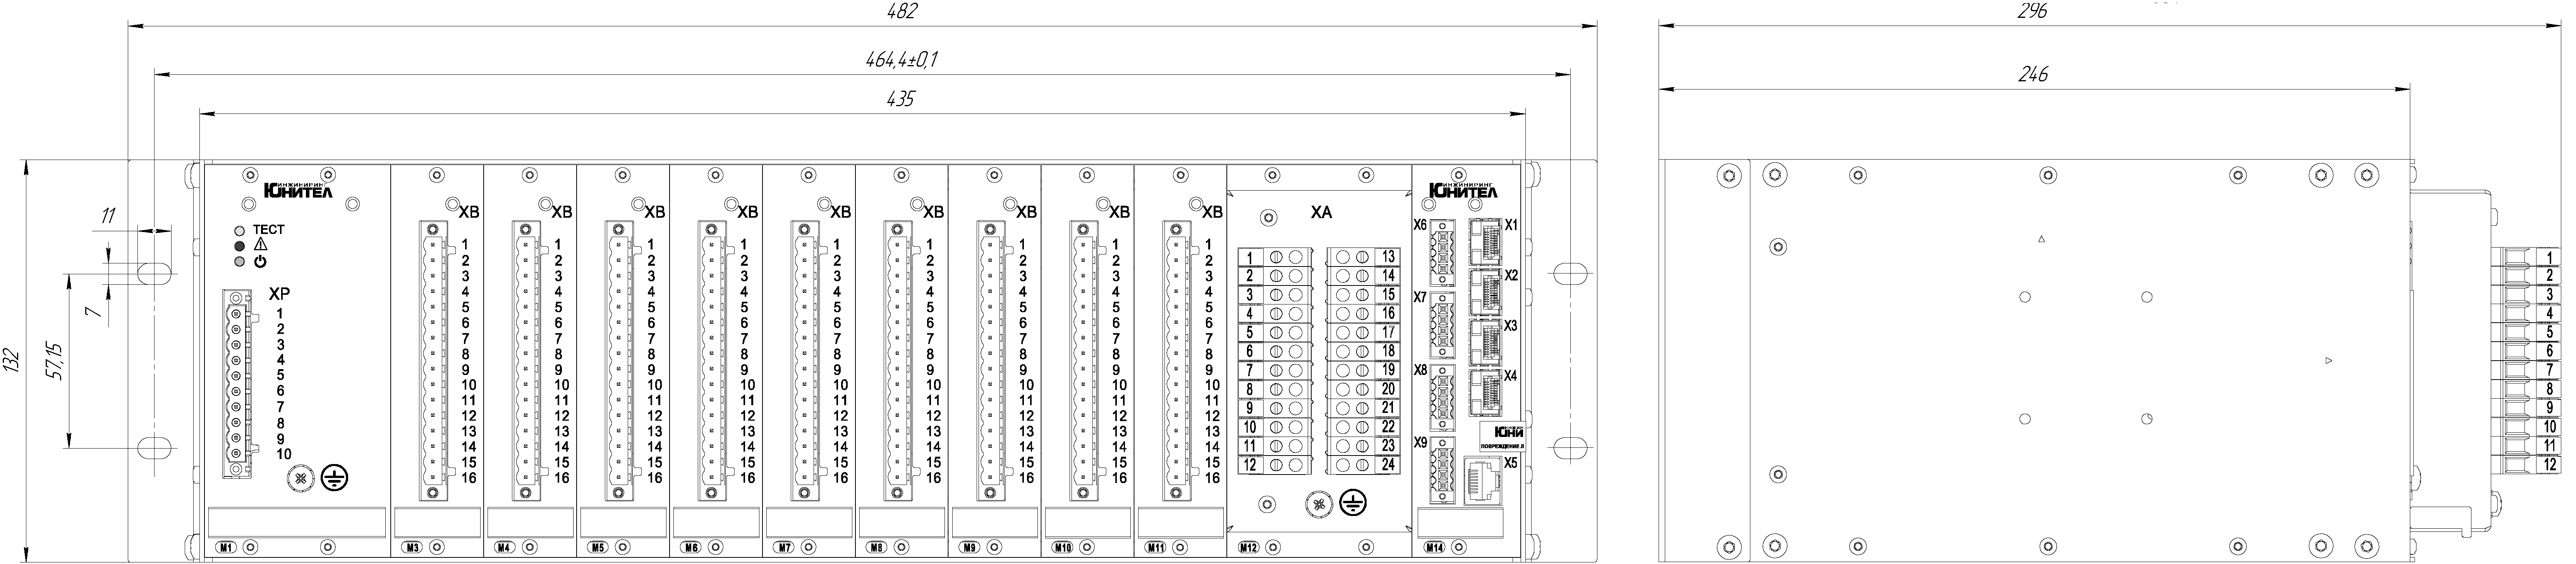
\includegraphics[width=1.4\textwidth]{img39.png}
  \caption{Габариты и установочные размеры устройства в исполнении ЮНИТ-М319-ДЗТ2 (I архитектура)}
  \label{fig:frontviewDZT2} % Опционально: ссылка на рисунок
\end{figure}

\begin{figure}[h!]
  \centering
  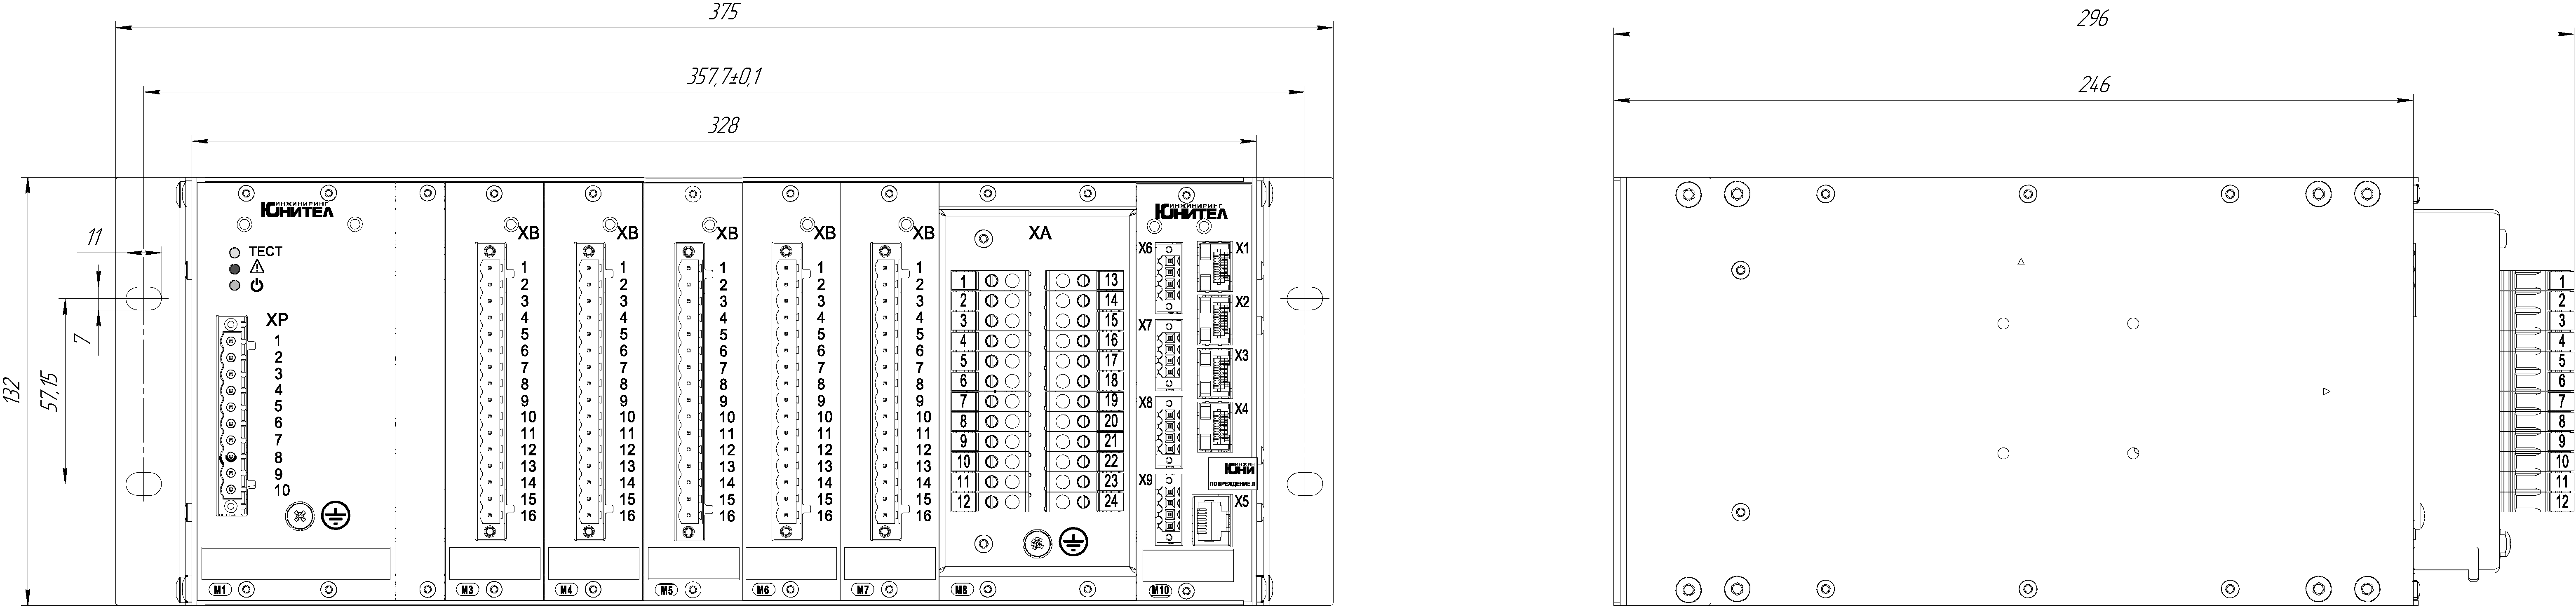
\includegraphics[width=1.4\textwidth]{img40.png}
  \caption{Габариты и установочные размеры устройства в исполнении ЮНИТ-М314-ДЗТ2 (II архитектура)}
  \label{fig:frontviewDZT22} % Опционально: ссылка на рисунок
\end{figure}

\clearpage

\end{landscape}
\restoregeometry


\newpage
\newpage

\KOMAoptions{paper=A3,paper=landscape}
\areaset{390mm}{270mm}
\fancyheadoffset{0pt} % обновляем хедер и футер

\topmargin=-2.6cm % Команда \topmargin задаёт верхнее поле страницы. При этом поле отсчитывается не от левого края листа, а от линии, параллельной краю листа и отстоящей от него на 1 дюйм
\oddsidemargin=0cm % отступ слева https://zns.susu.ru/IT/latex/Marking/marking.html
\headsep=0cm
\footskip=45pt
\setlength{\headheight}{1cm}

\color{uniblue}{\section[(справочное) Структурно-функциональная схема устройства]{(справочное)\\Структурно-функциональная схема устройства}\label{app:fsu}}
\color{black}

\begin{figure}[H]
\centering
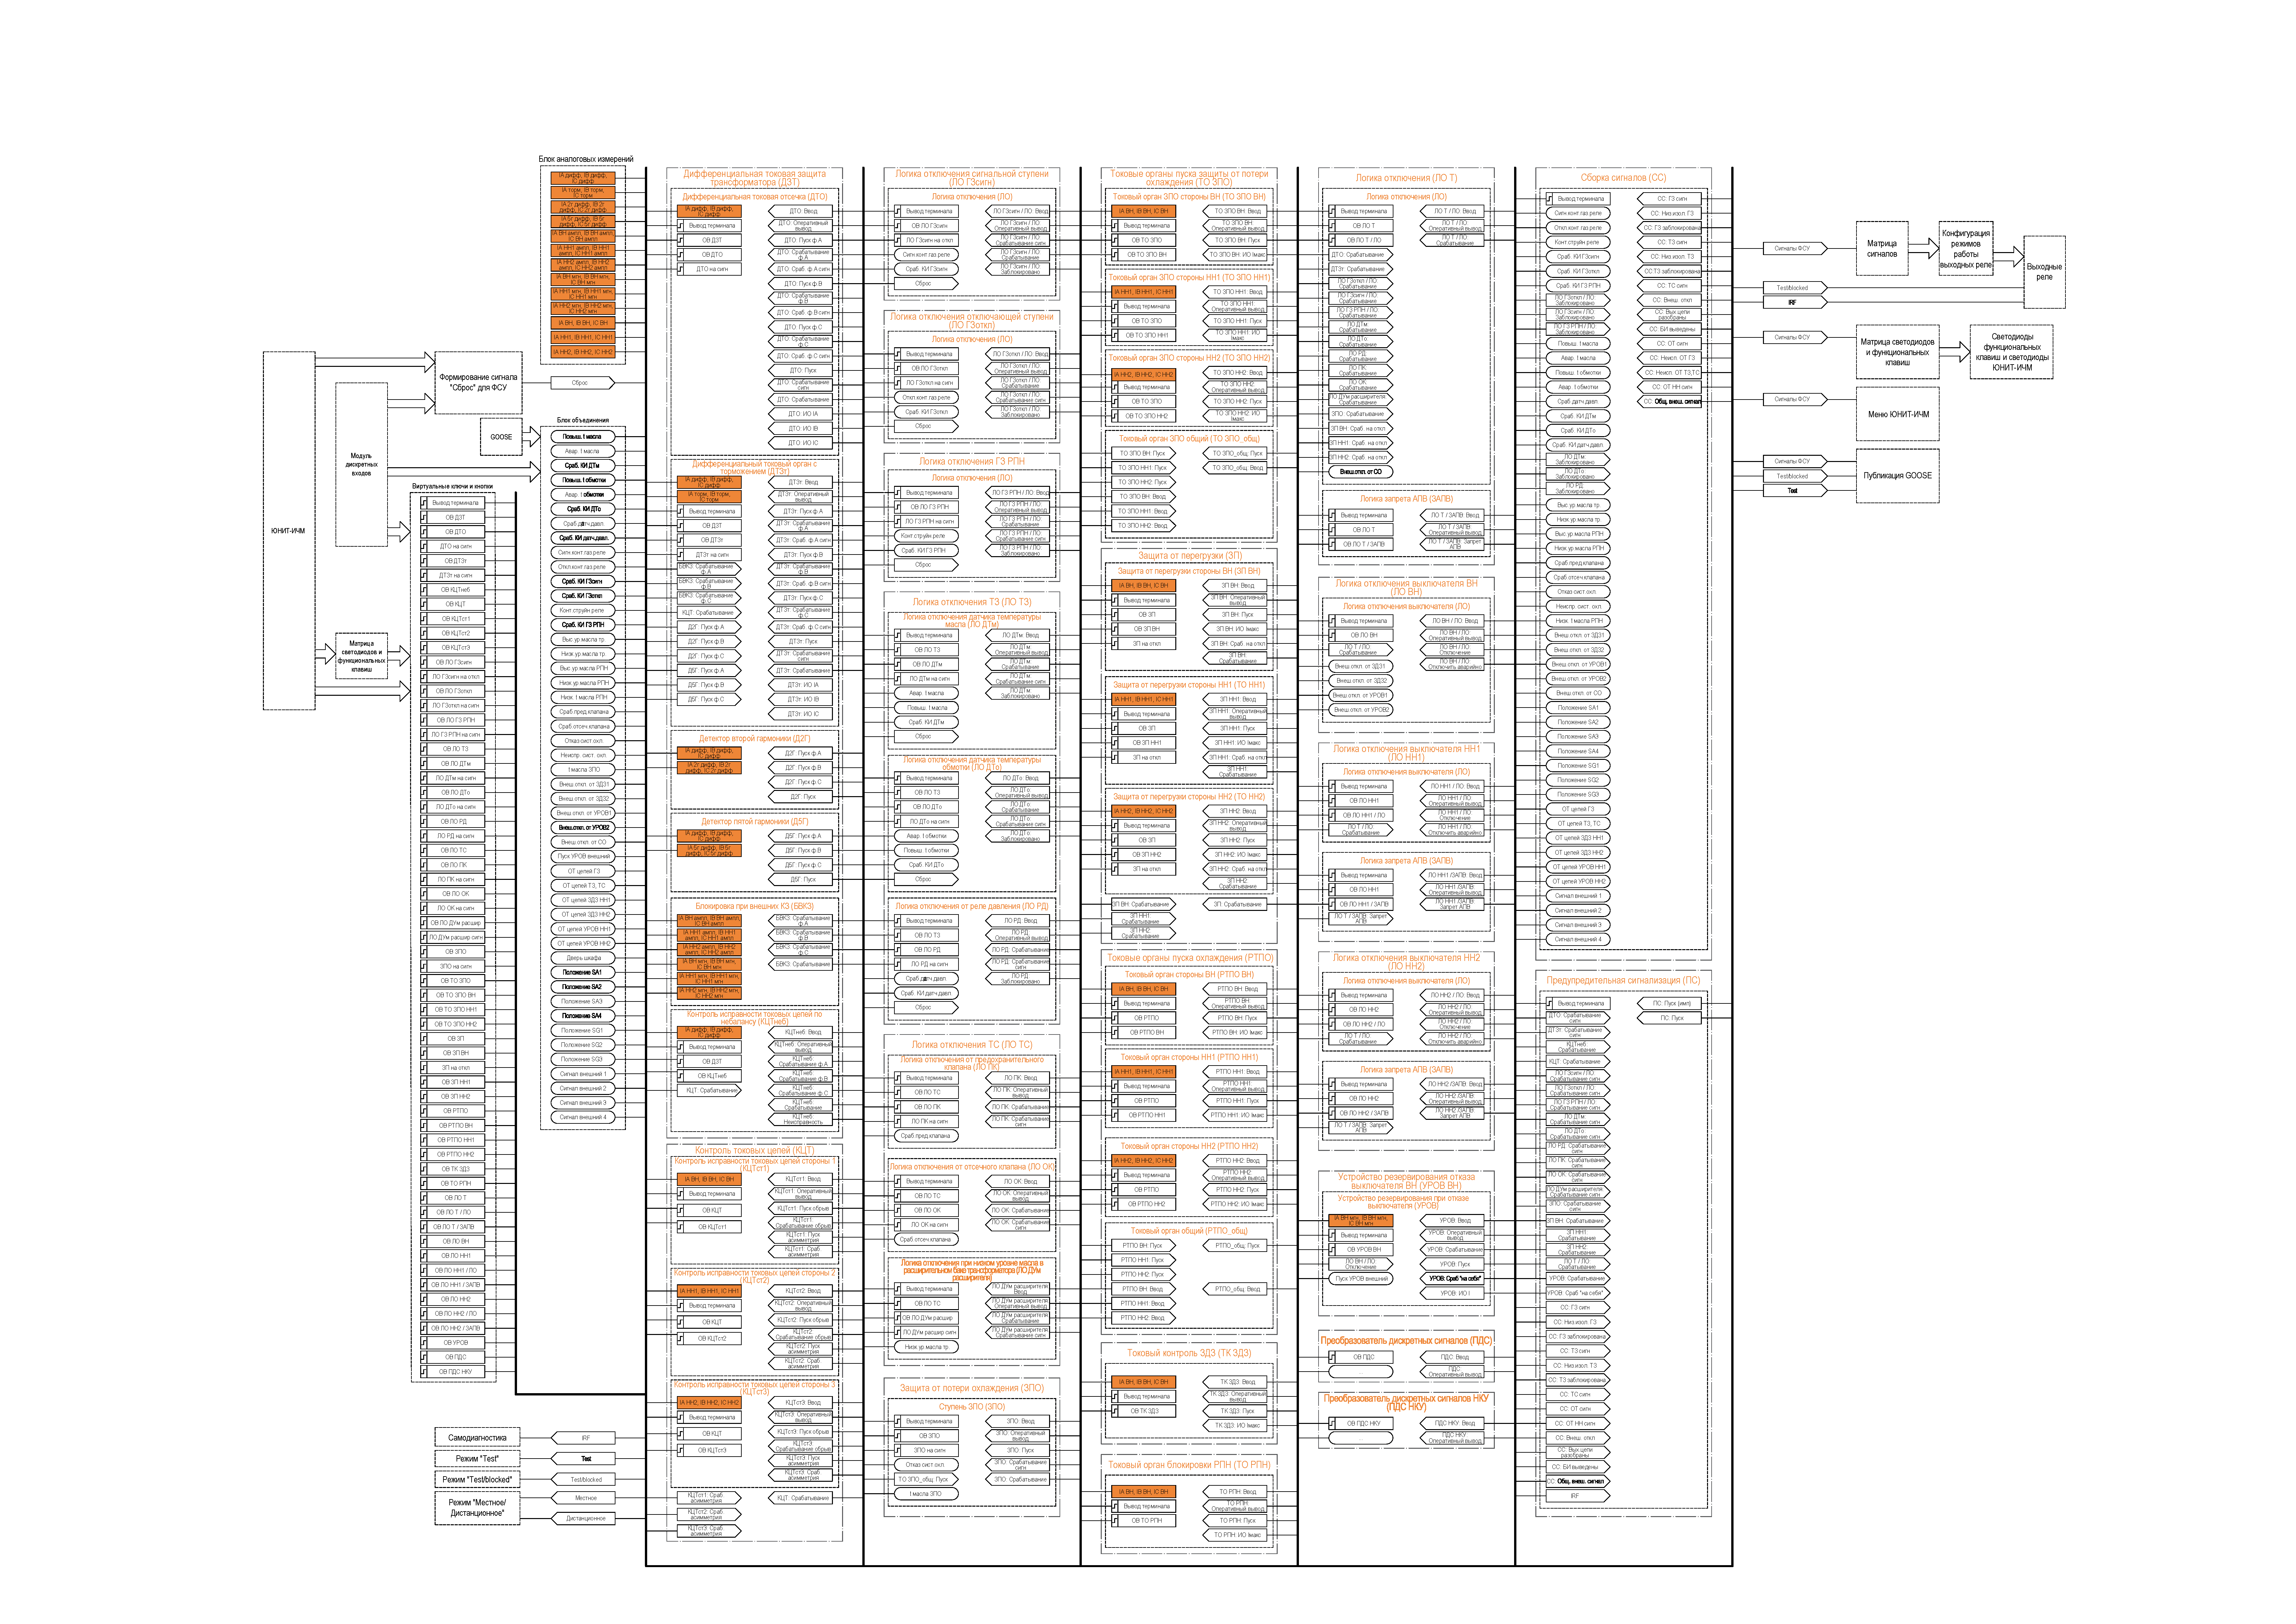
\includegraphics[width=0.85\textwidth,height=0.85\textheight,keepaspectratio]{img41.pdf}
\end{figure}

\clearpage %!!!!!!!!!!БЕЗ ЭТОЙ СТРОЧКИ ХРЕНЬ



\newpage
\KOMAoption{paper}{a4, portrait}
\areaset{267mm}{180mm}
\fancyheadoffset{0pt} % обновляем хедер и футер

\newgeometry{
  top=14mm,
  bottom=11mm,
  right=10mm,
  left=22mm,
}

\begin{landscape}

\setlength{\footskip}{15.5pt}

\color{uniblue}{\section[(справочное) Подключение аналоговых цепей трансформаторов тока и напряжения к устройству]{(справочное)\\Подключение аналоговых цепей трансформаторов тока и напряжения к устройству}\label{app:analogs}}
\color{black}

\begin{figure}[h!]
  \centering
  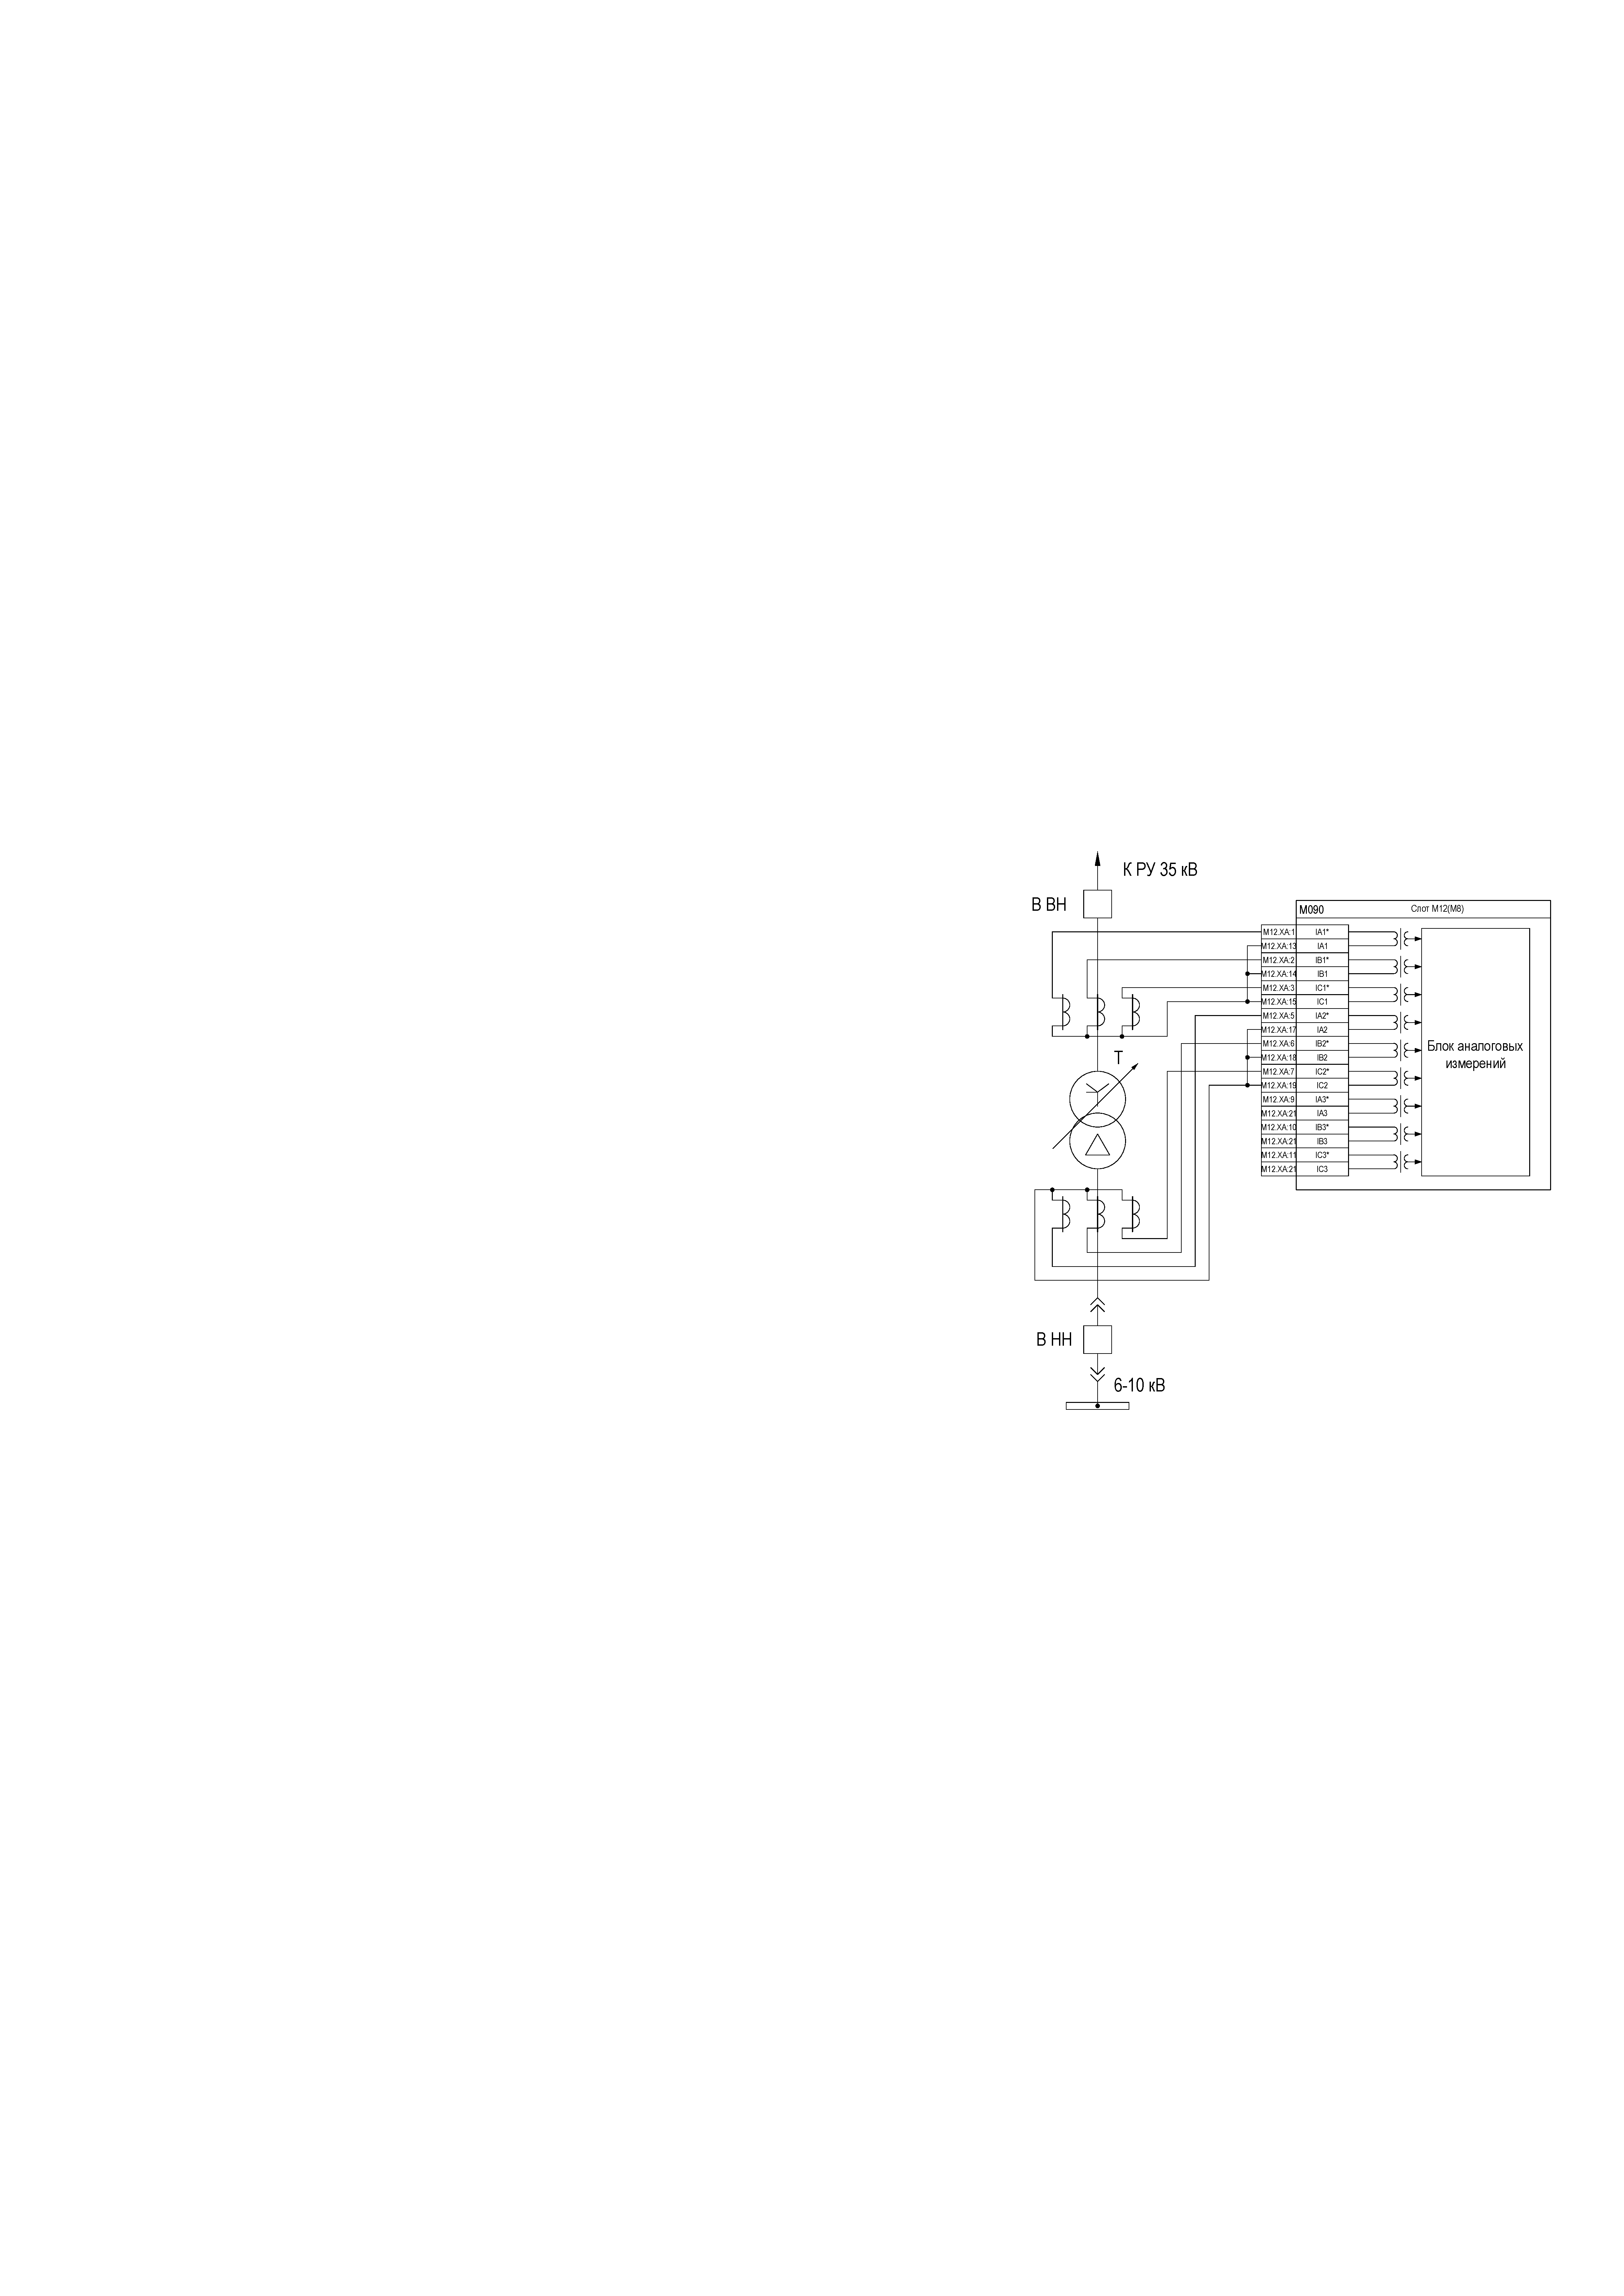
\includegraphics[width=0.82\textwidth]{img42.pdf}
  \caption{Подключение аналоговых цепей трансформаторов тока двухобмоточного трансформатора 35 кВ к устройству}
  \label{analogs:fig1} % Опционально: ссылка на рисунок
\end{figure}

\begin{figure}[h!]
  \centering
  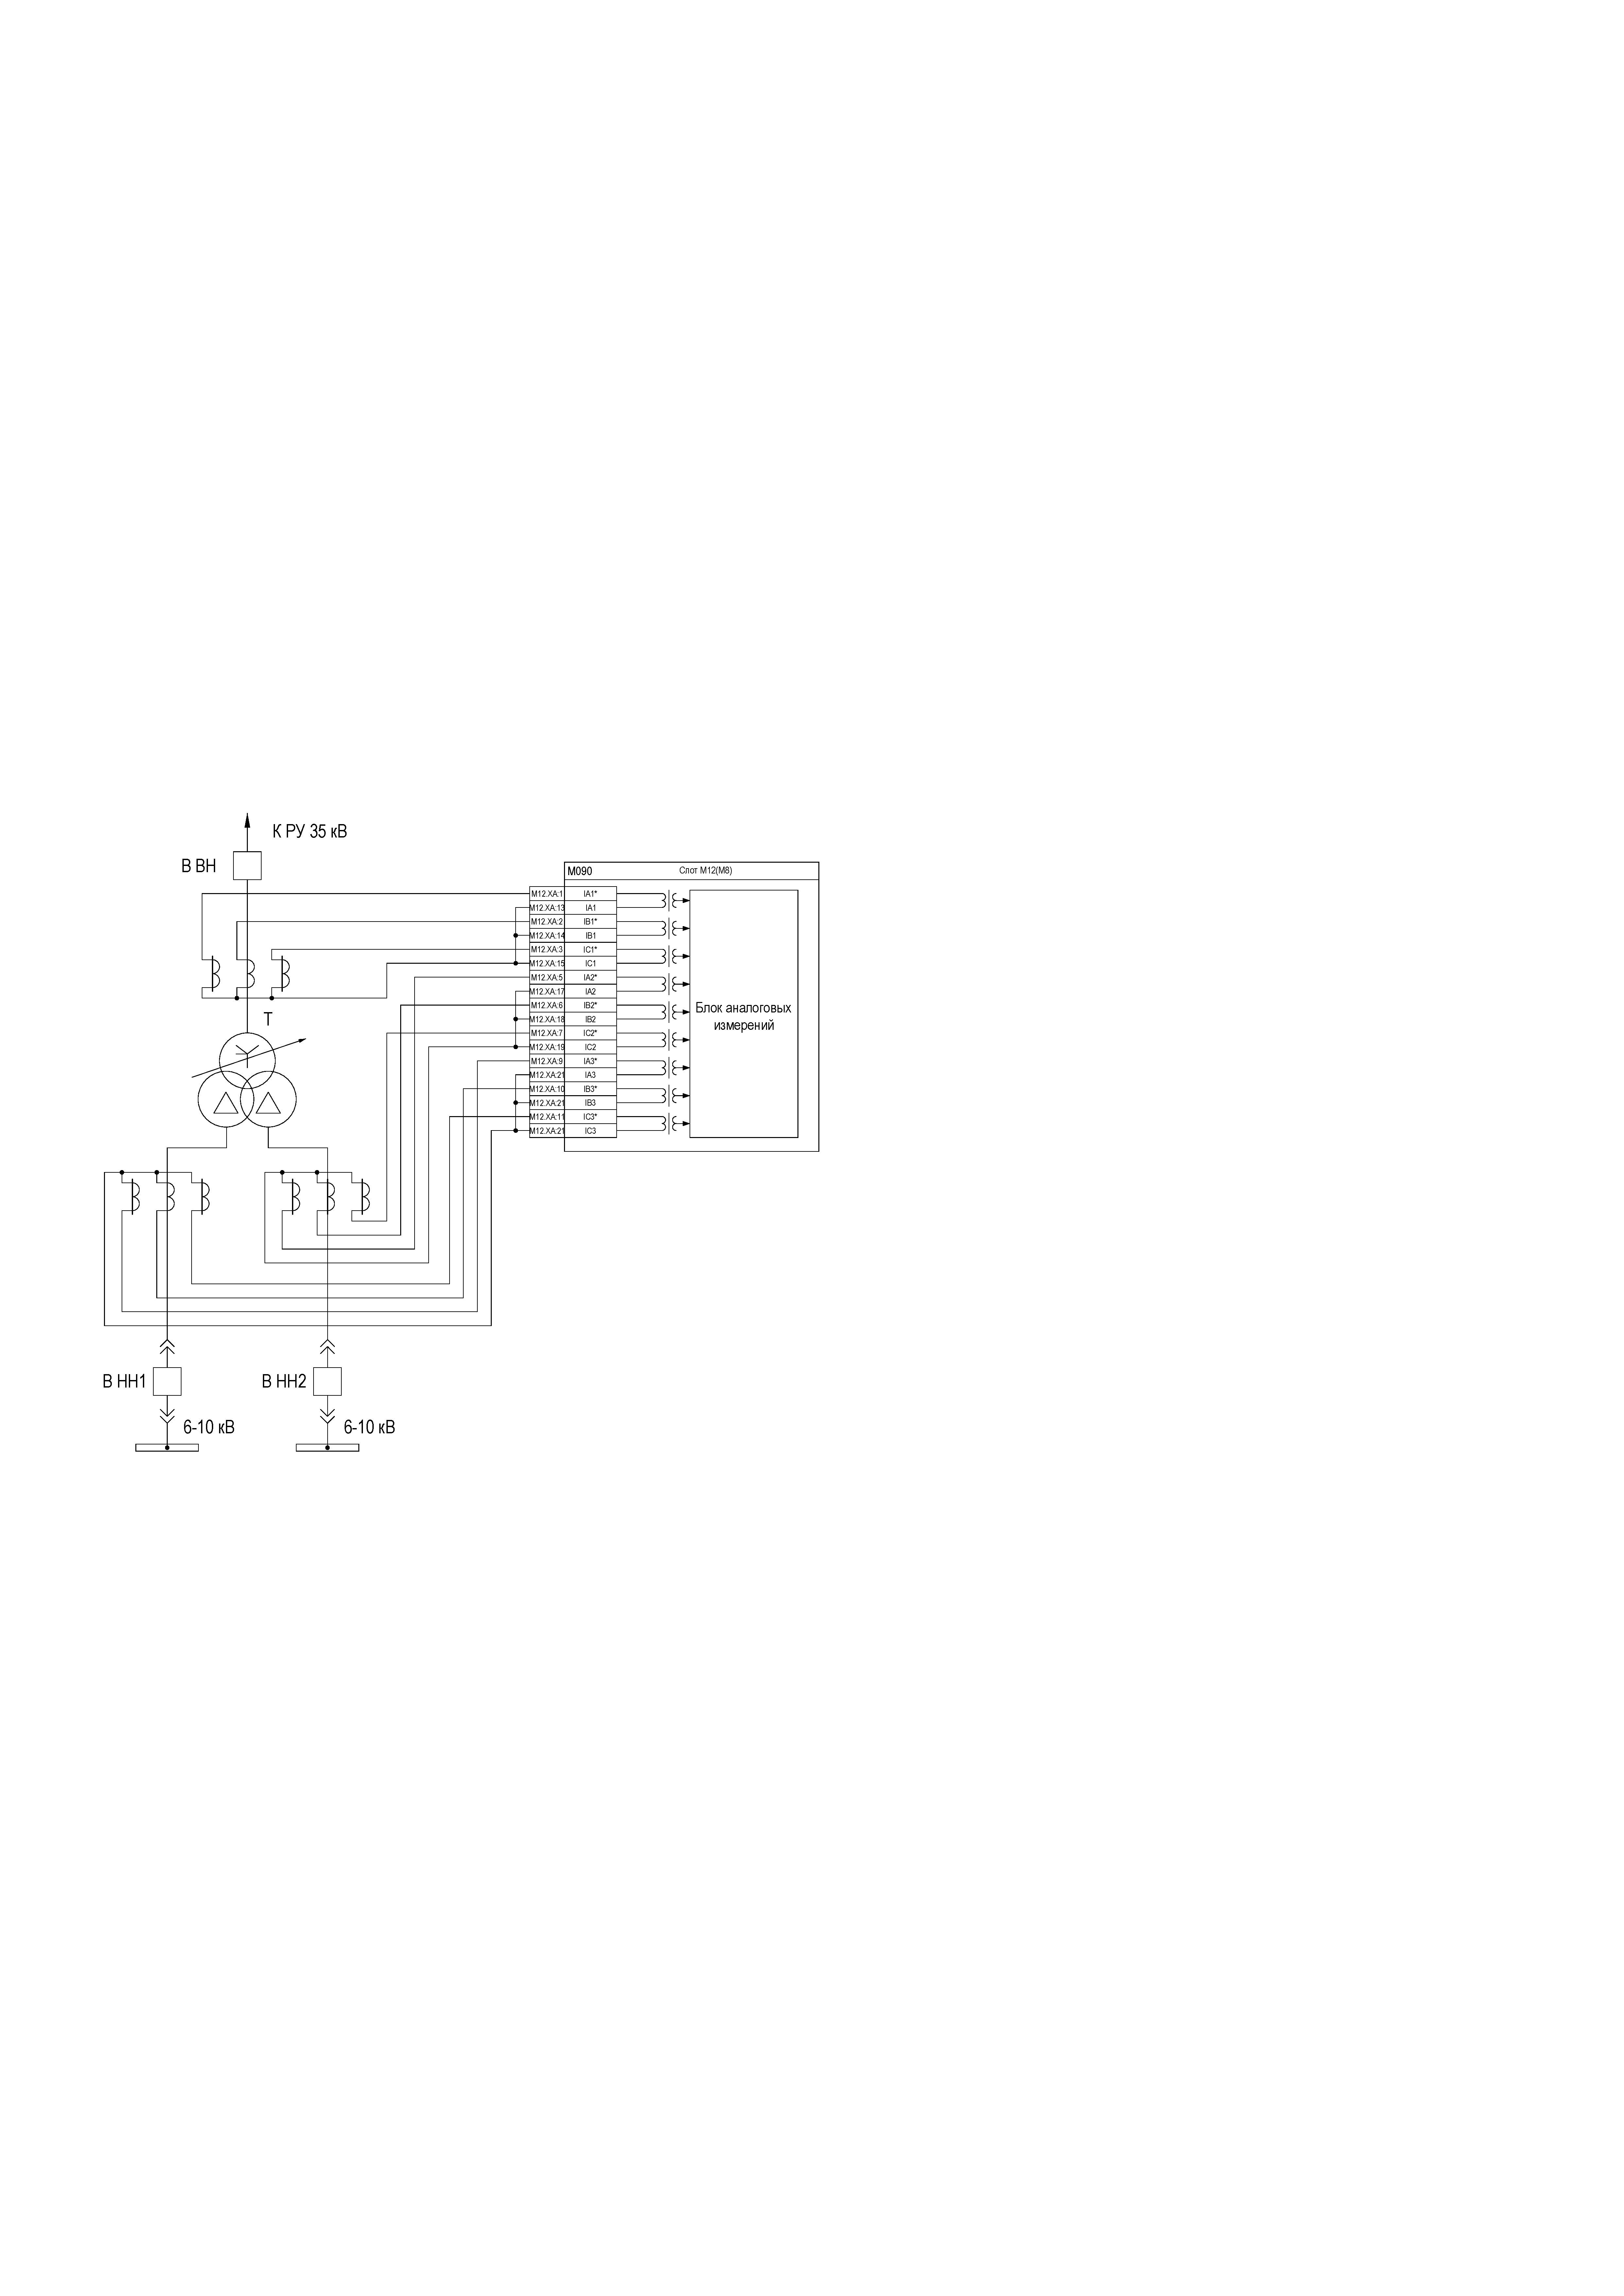
\includegraphics[width=0.9\textwidth]{img43.pdf}
  \caption{Подключение аналоговых цепей трансформаторов тока трансформатора 35 кВ с расщепленной обмоткой низшего напряжения к устройству}
  \label{analogs:fig2} % Опционально: ссылка на рисунок
\end{figure}

\clearpage
\end{landscape}
\restoregeometry


\newpage
\KOMAoption{paper}{a4, portrait}
\areaset{267mm}{180mm}
\fancyheadoffset{0pt} % обновляем хедер и футер

\newgeometry{
  top=14mm,
  bottom=11mm,
  right=10mm,
  left=22mm,
}

\begin{landscape}

\setlength{\footskip}{15.5pt}

\color{uniblue}{\section[(обязательное) Подключение дискретных входов и выходов устройства к внутренним цепям алгоритмов для архитектуры I типа]{(обязательное)\\Подключение дискретных входов и выходов устройства к внутренним цепям алгоритмов для архитектуры I типа}\label{app:inouts}}
\color{black}


\begin{figure}[h!]
  \centering
  \hspace*{-1cm} % Сдвигаем рисунок влево на 2 см  
  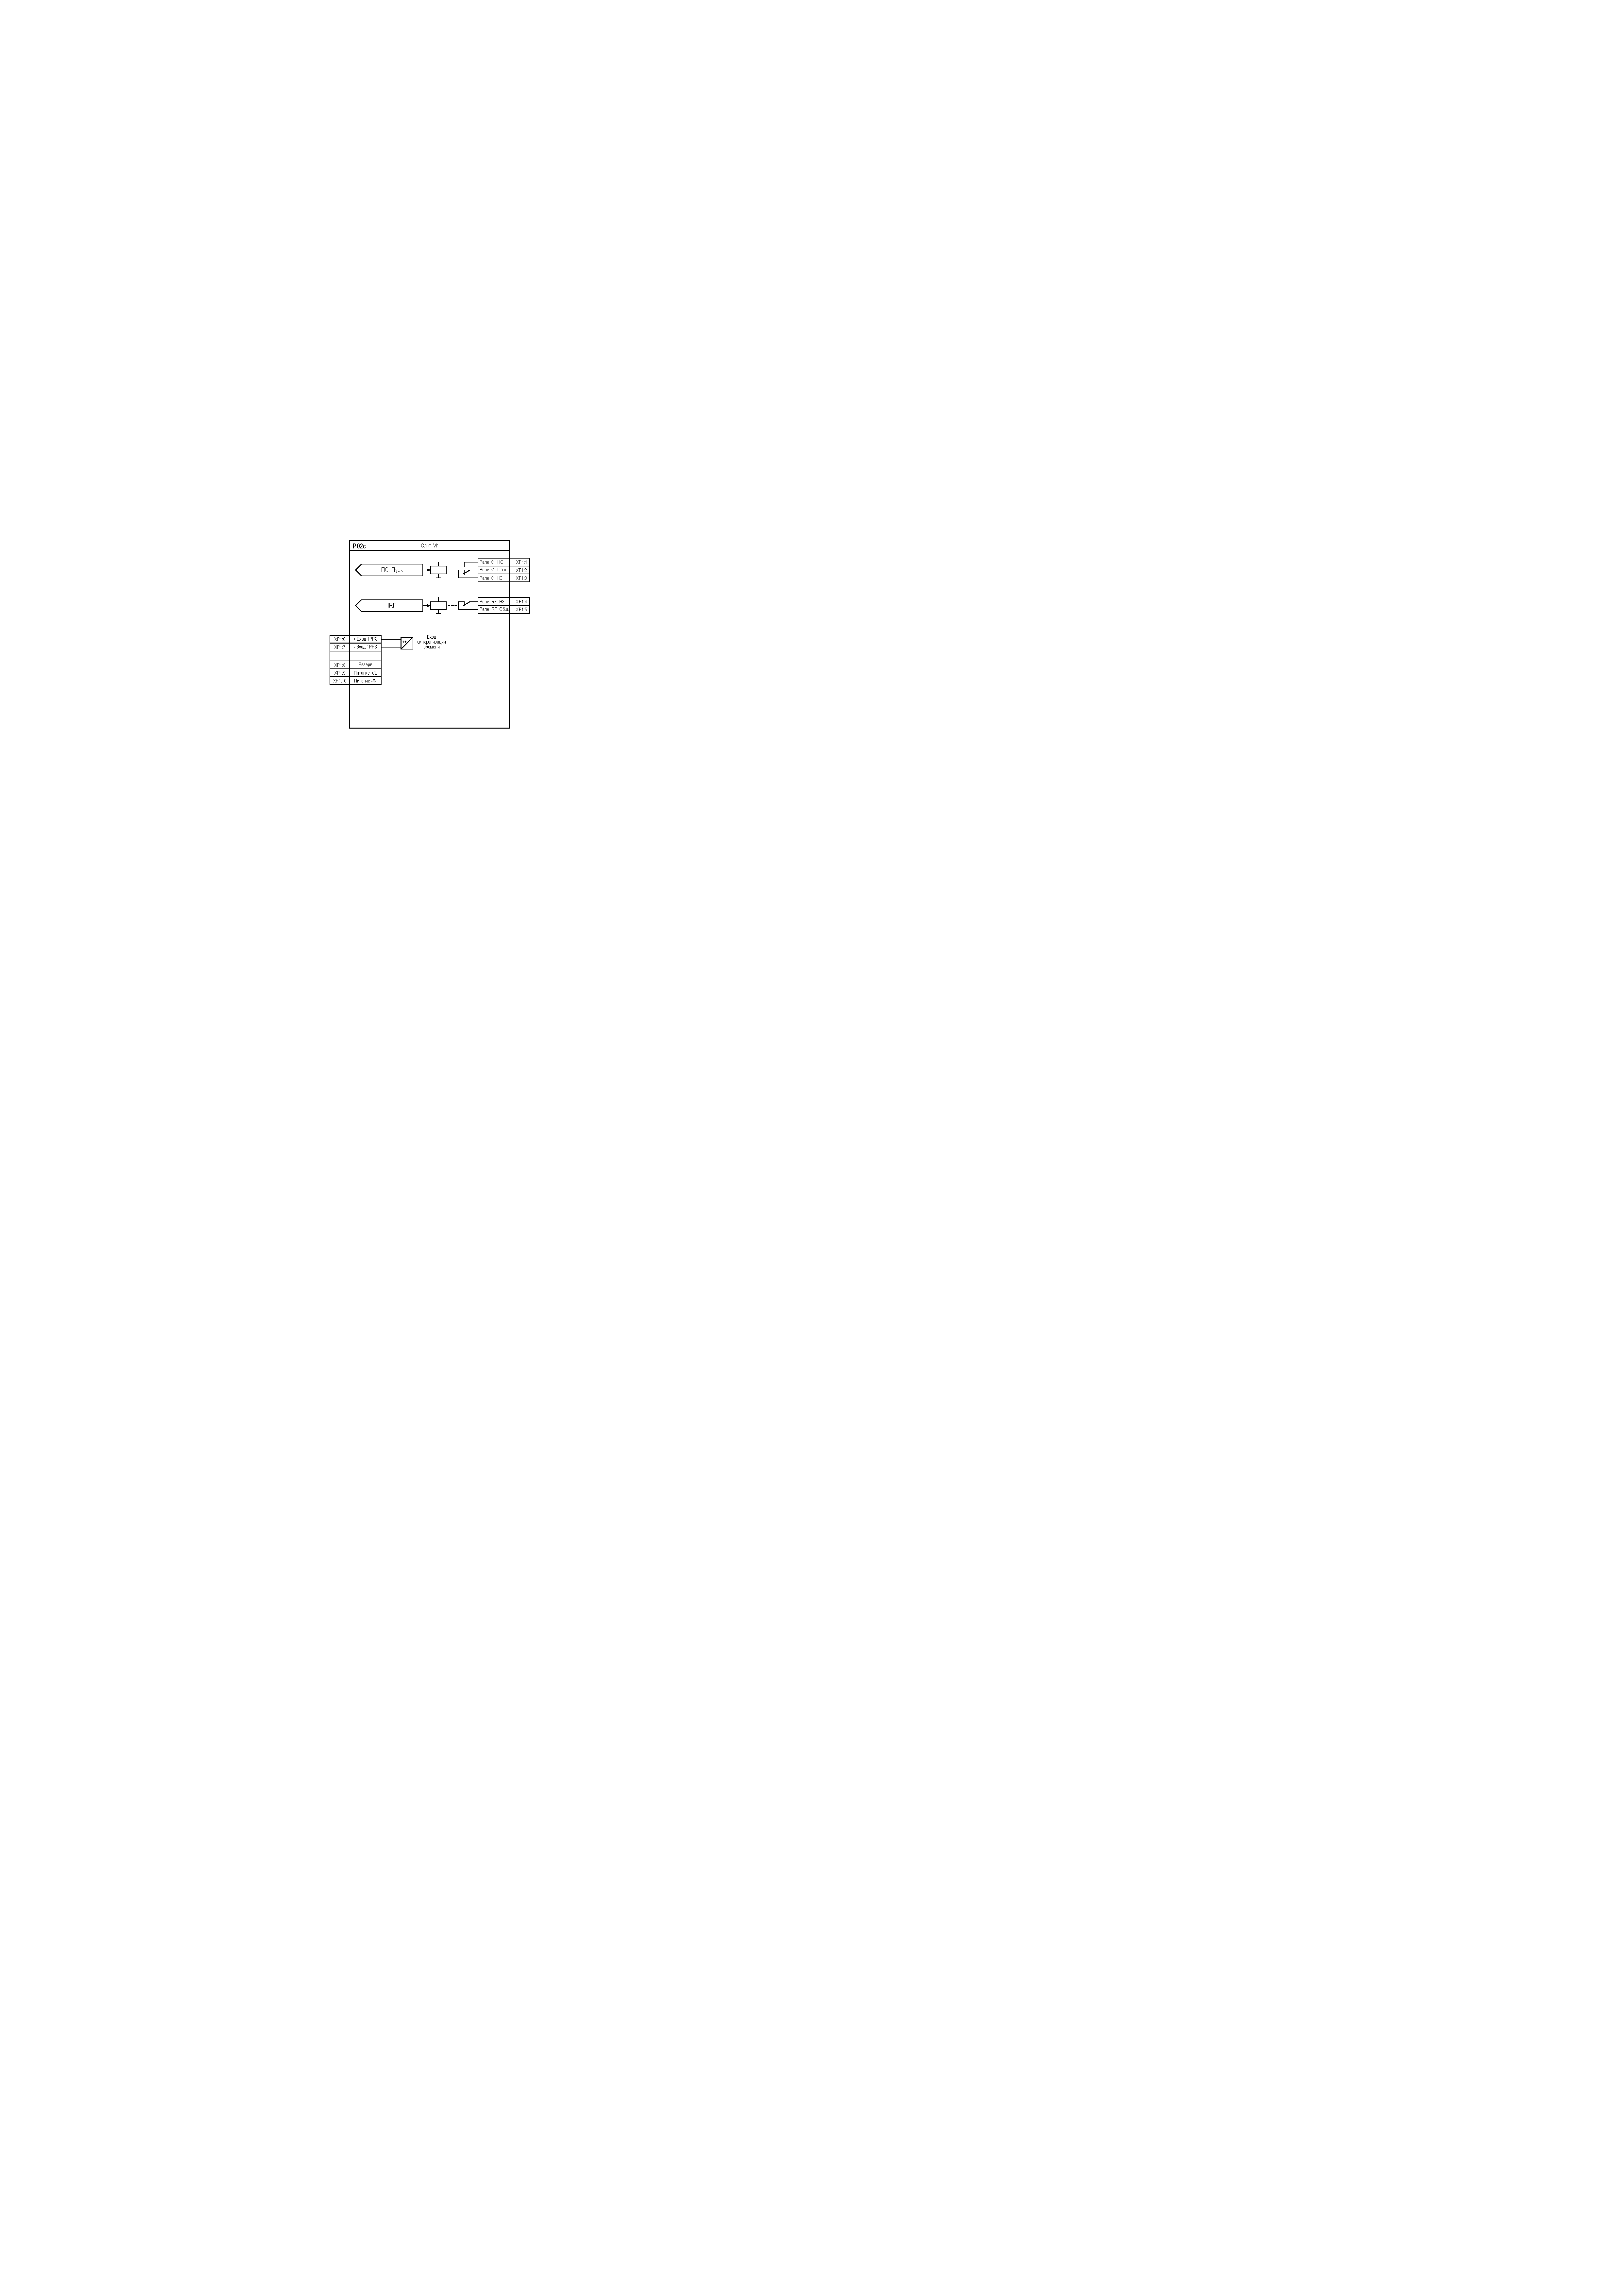
\includegraphics[width=1.5\textwidth]{img44.pdf}
  \caption{Подключение дискретных входов и выходов к внутренним сигналам алгоритмов для платы в слоте М1}
  \label{fig:sig1} % Опционально: ссылка на рисунок
\end{figure}

\begin{figure}[h!]
  \centering
  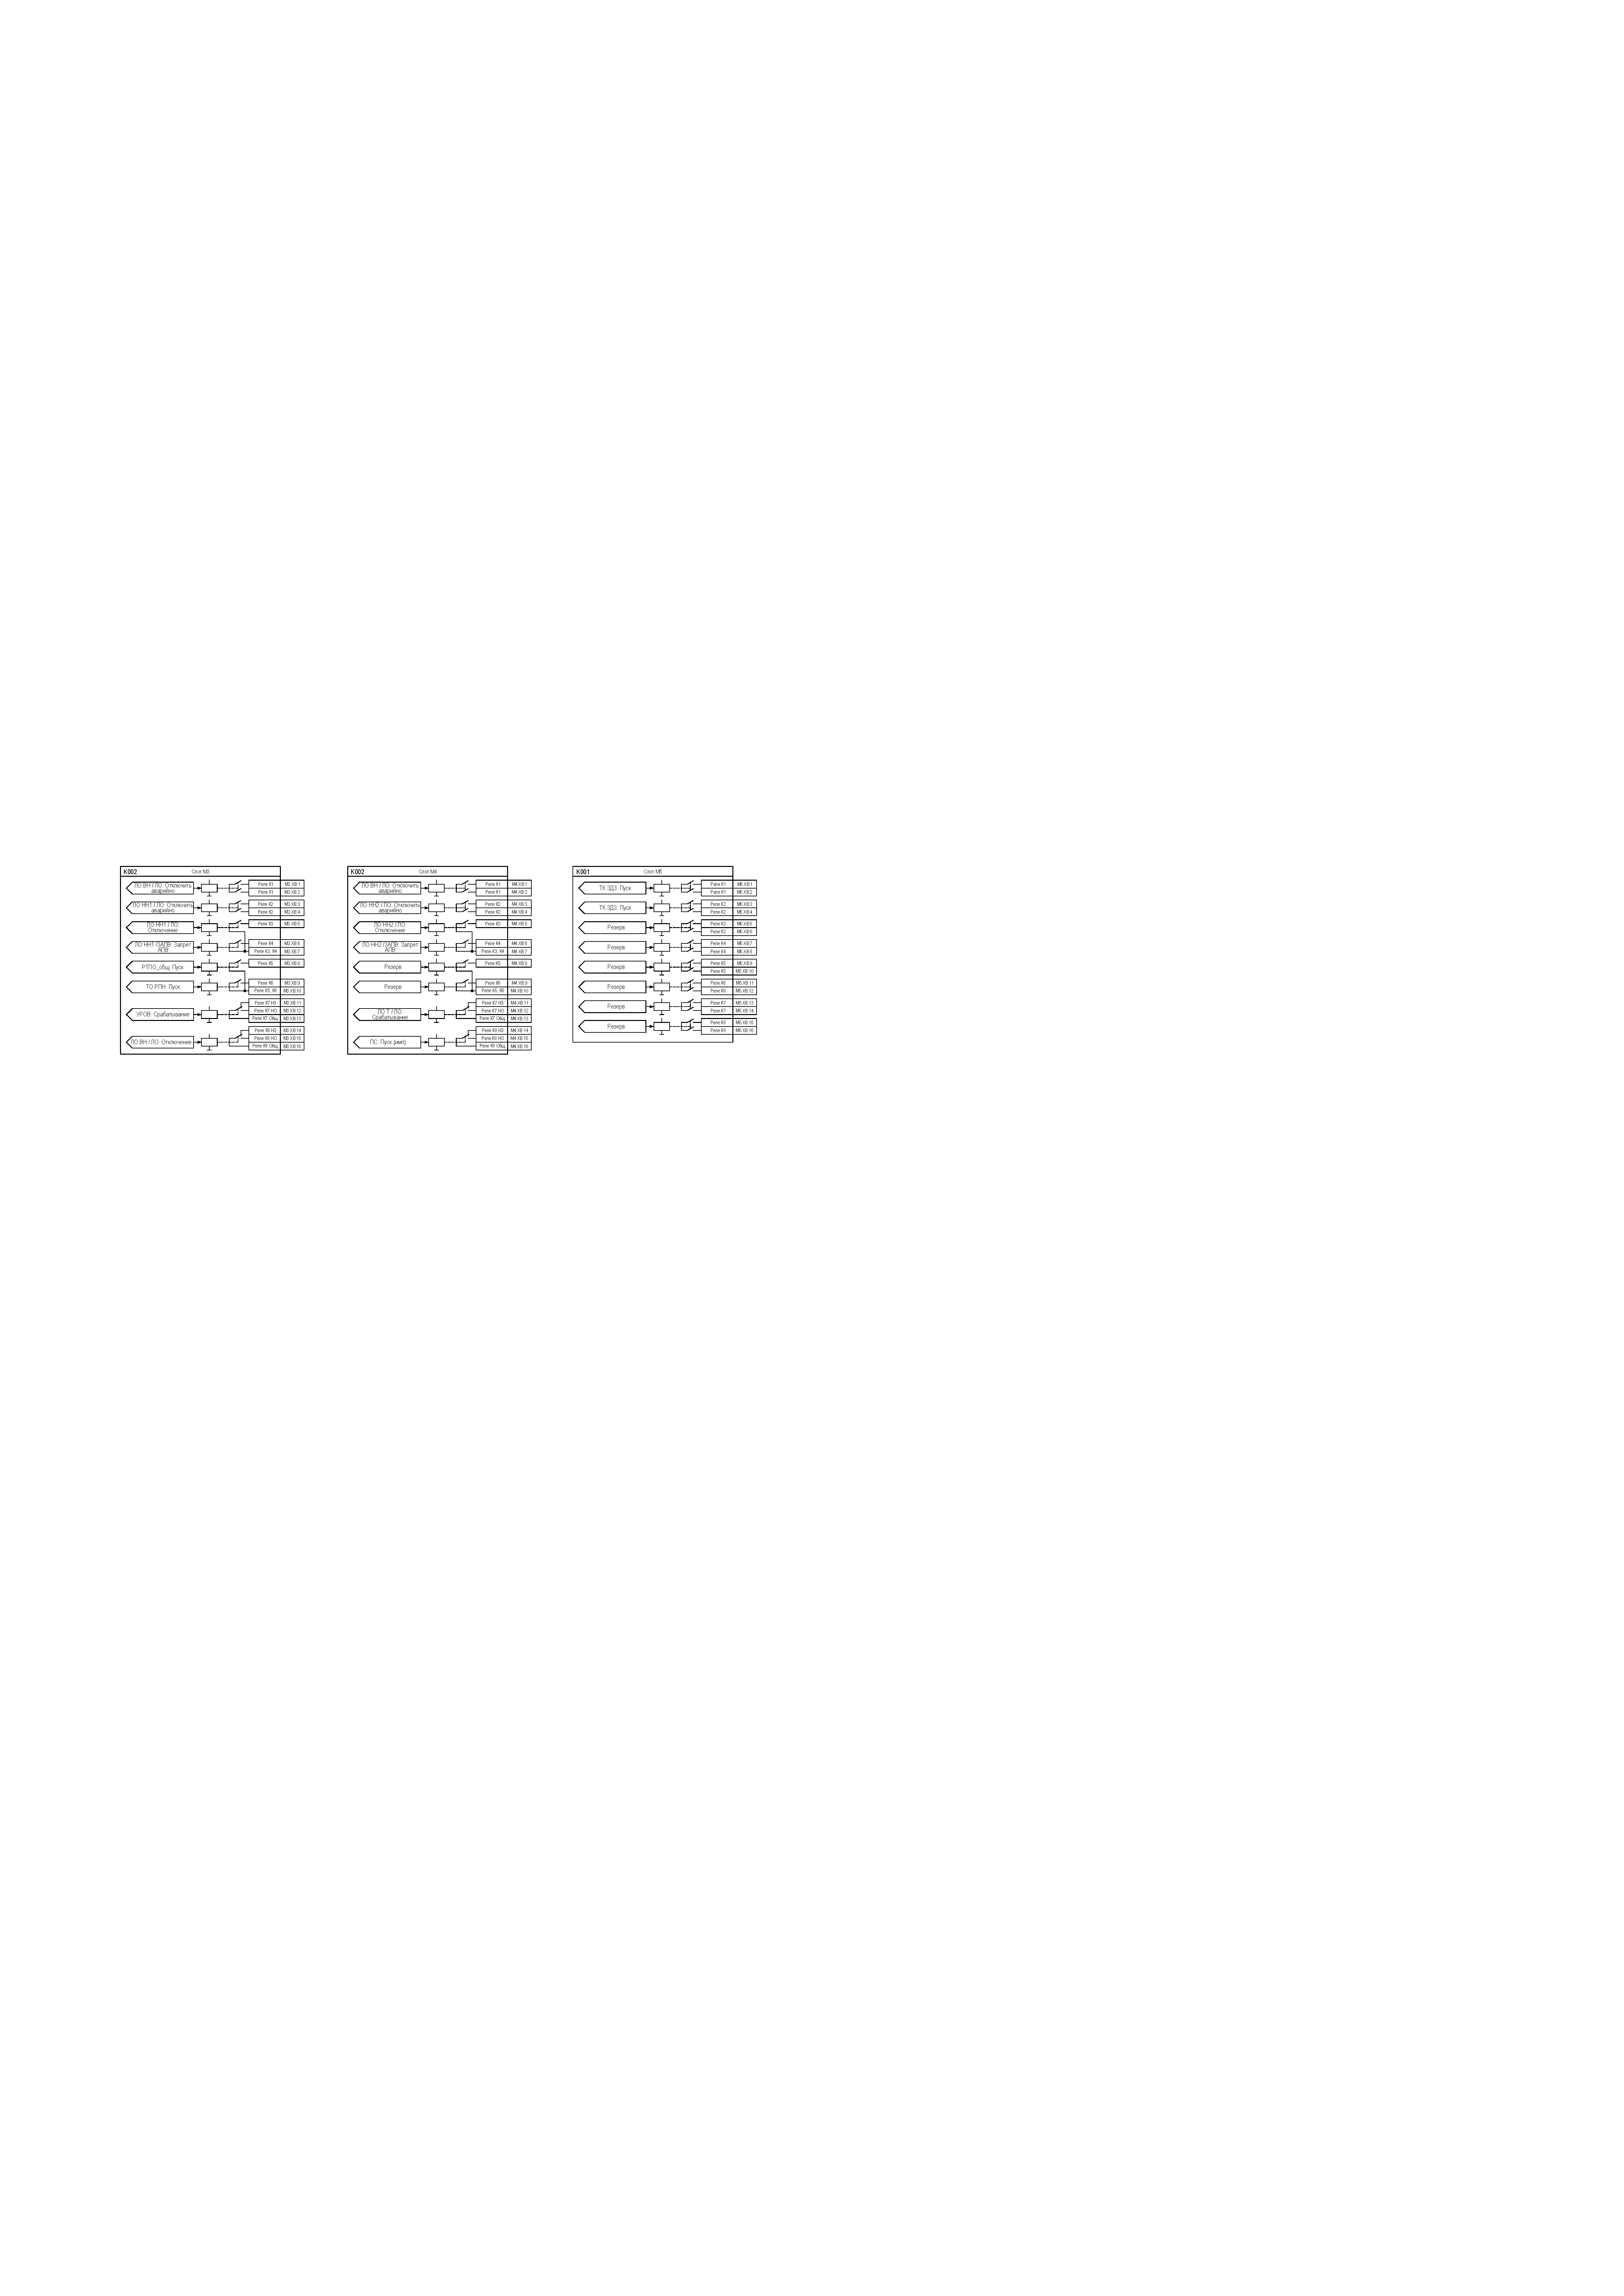
\includegraphics[width=1.45\textwidth]{img45.pdf}
  \caption{Подключение дискретных входов и выходов к внутренним сигналам алгоритмов для плат в слотах М3-М5}
  \label{fig:sig2} % Опционально: ссылка на рисунок
\end{figure}

\begin{figure}[h!]
  \centering
  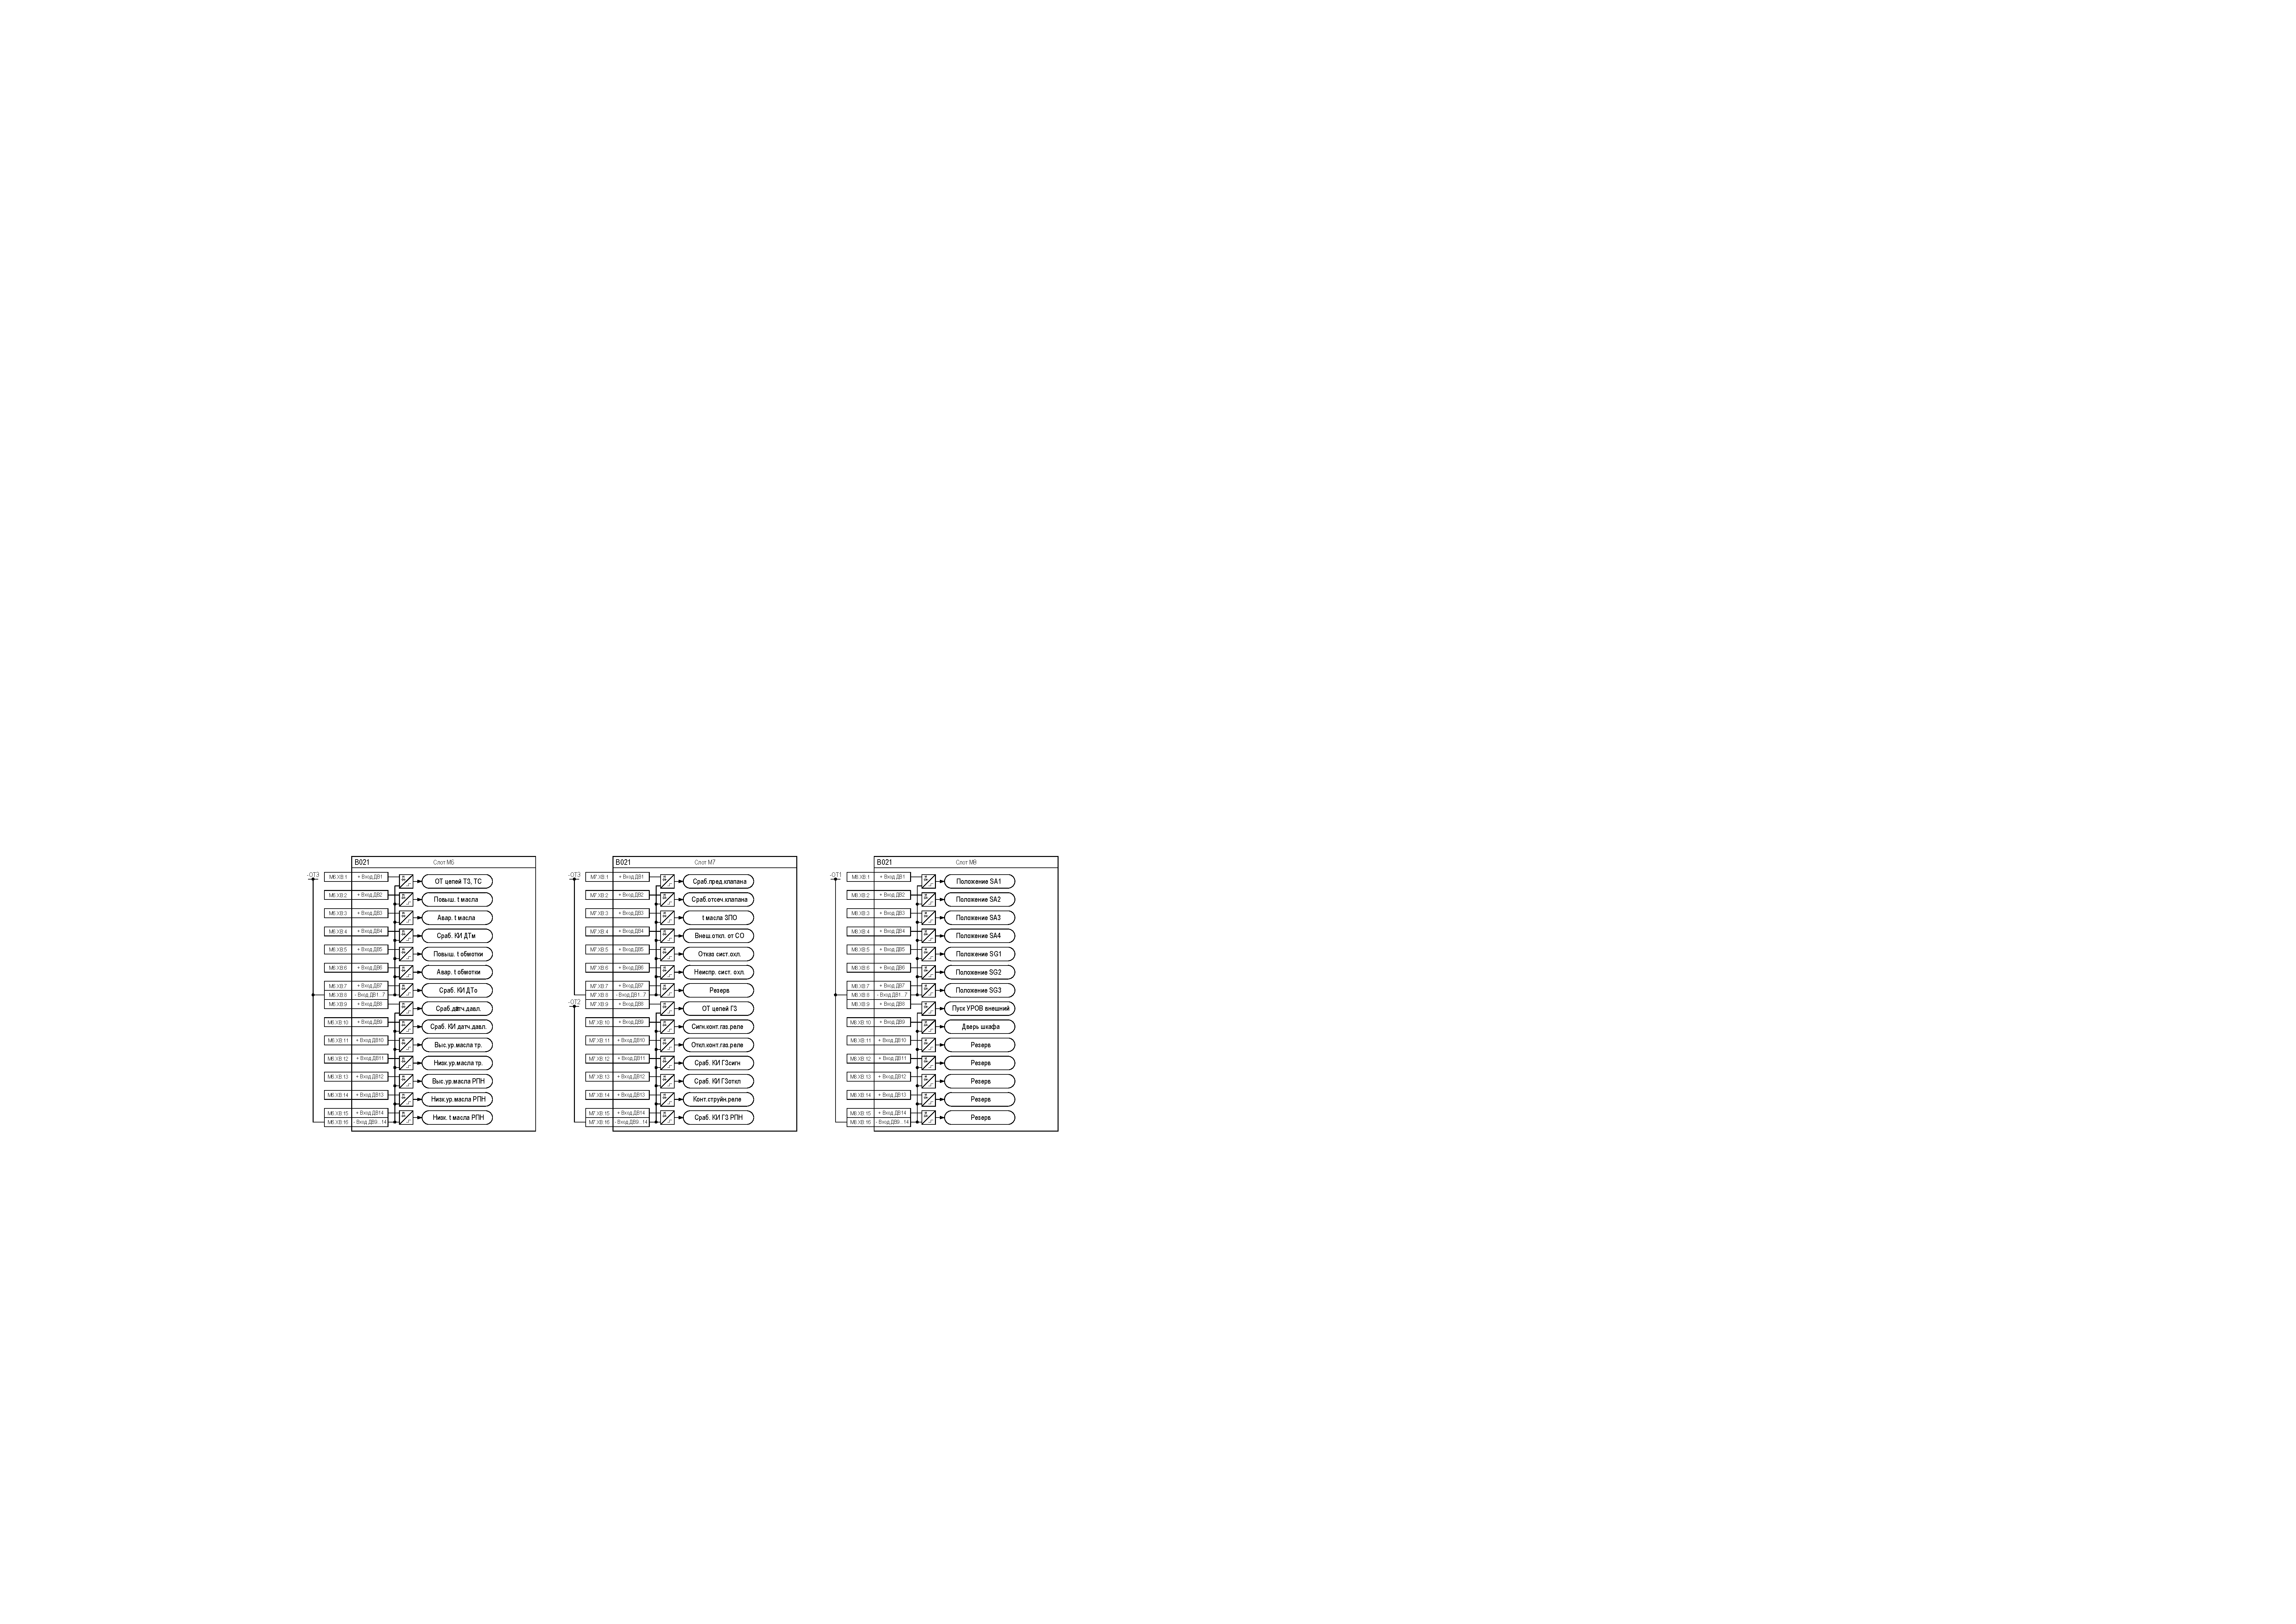
\includegraphics[width=1.4\textwidth]{img46.pdf}
  \caption{Подключение дискретных входов и выходов к внутренним сигналам алгоритмов для плат в слотах М6-М8}
  \label{fig:sig3} % Опционально: ссылка на рисунок
\end{figure}

\begin{figure}[h!]
  \centering
  
\includegraphics[width=1.5\textwidth]{img47.pdf}
  \caption{Подключение дискретных входов и выходов к внутренним сигналам алгоритмов для платы в слоте М9}
  \label{fig:sig4} % Опционально: ссылка на рисунок
\end{figure}


\clearpage
\end{landscape}
\restoregeometry


\newpage
\KOMAoption{paper}{a4, portrait}
\areaset{267mm}{180mm}
\fancyheadoffset{0pt} % обновляем хедер и футер

\newgeometry{
  top=14mm,
  bottom=11mm,
  right=10mm,
  left=22mm,
}

\begin{landscape}

\setlength{\footskip}{15.5pt}

\color{uniblue}{\section[(обязательное) Подключение дискретных входов и выходов устройства к внутренним цепям алгоритмов для архитектуры II типа]{(обязательное)\\Подключение дискретных входов и выходов устройства к внутренним цепям алгоритмов для архитектуры II типа}\label{app:inouts2}}
\color{black}


\begin{figure}[h!]
  \centering
  \hspace*{-1cm} % Сдвигаем рисунок влево на 2 см  
  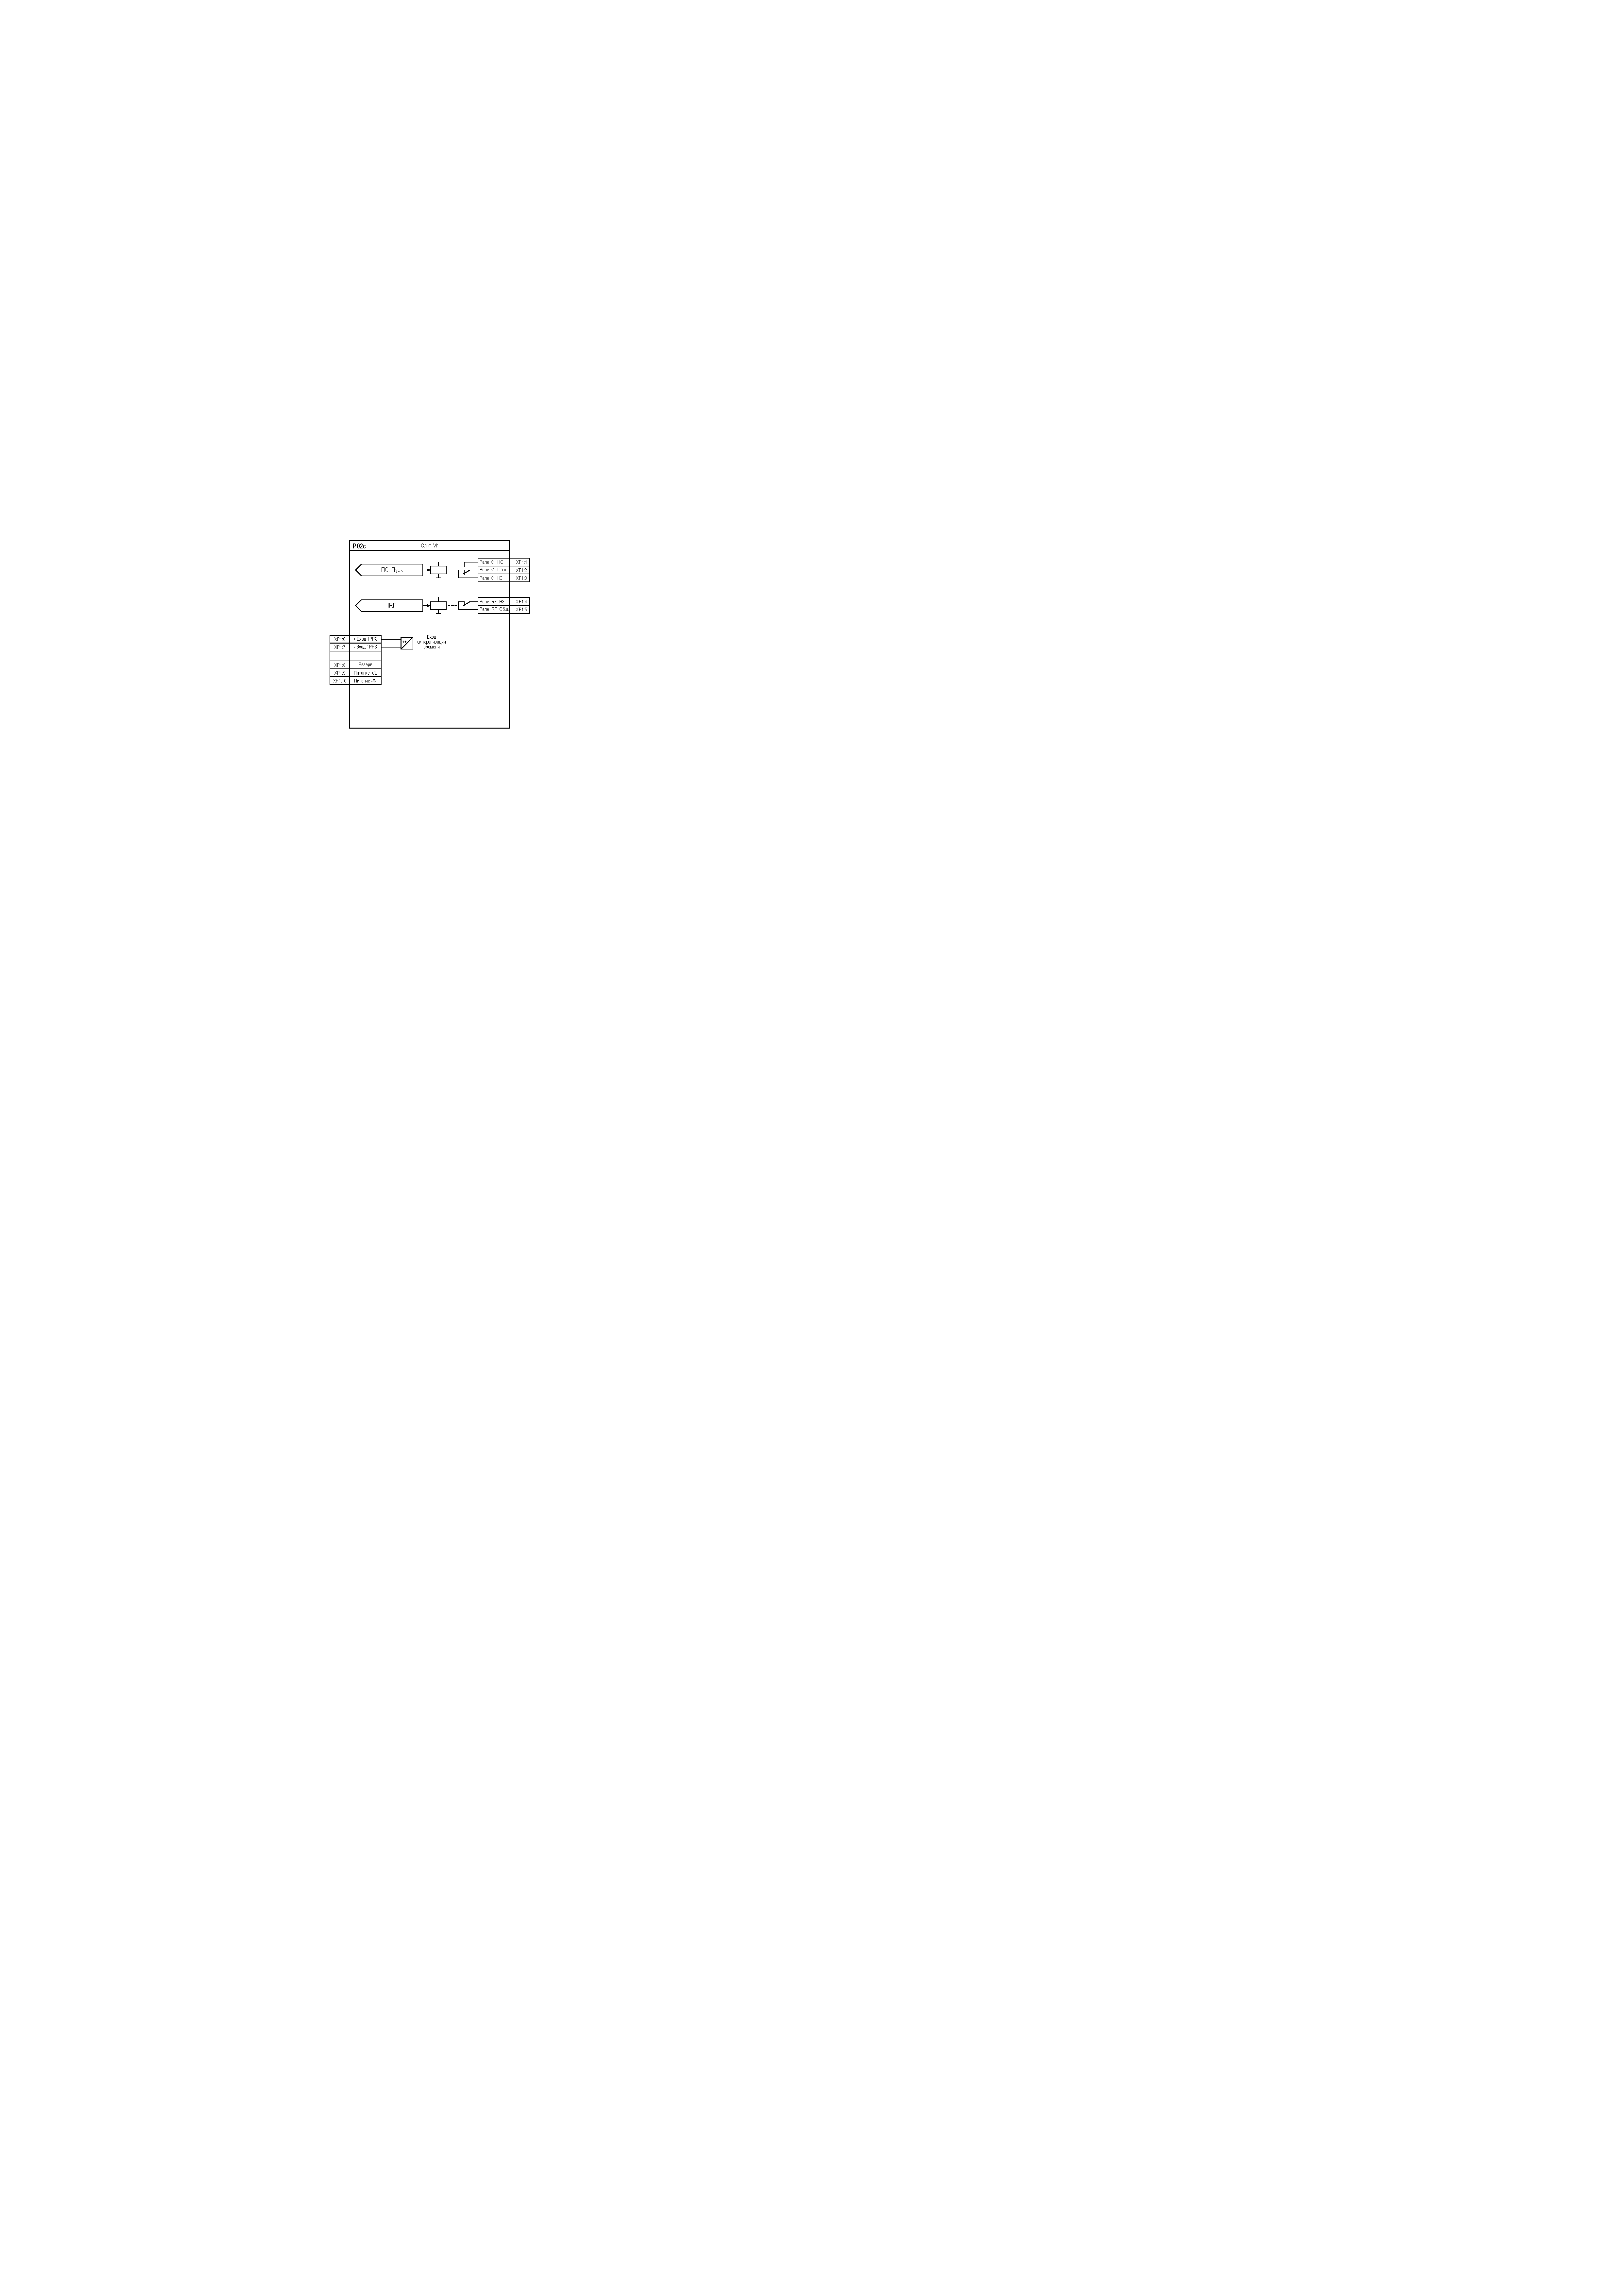
\includegraphics[width=1.5\textwidth]{img48.pdf}
  \caption{Подключение дискретных входов и выходов к внутренним сигналам алгоритмов для платы в слоте М1}
  \label{fig:sig21} % Опционально: ссылка на рисунок
\end{figure}

\begin{figure}[h!]
  \centering
  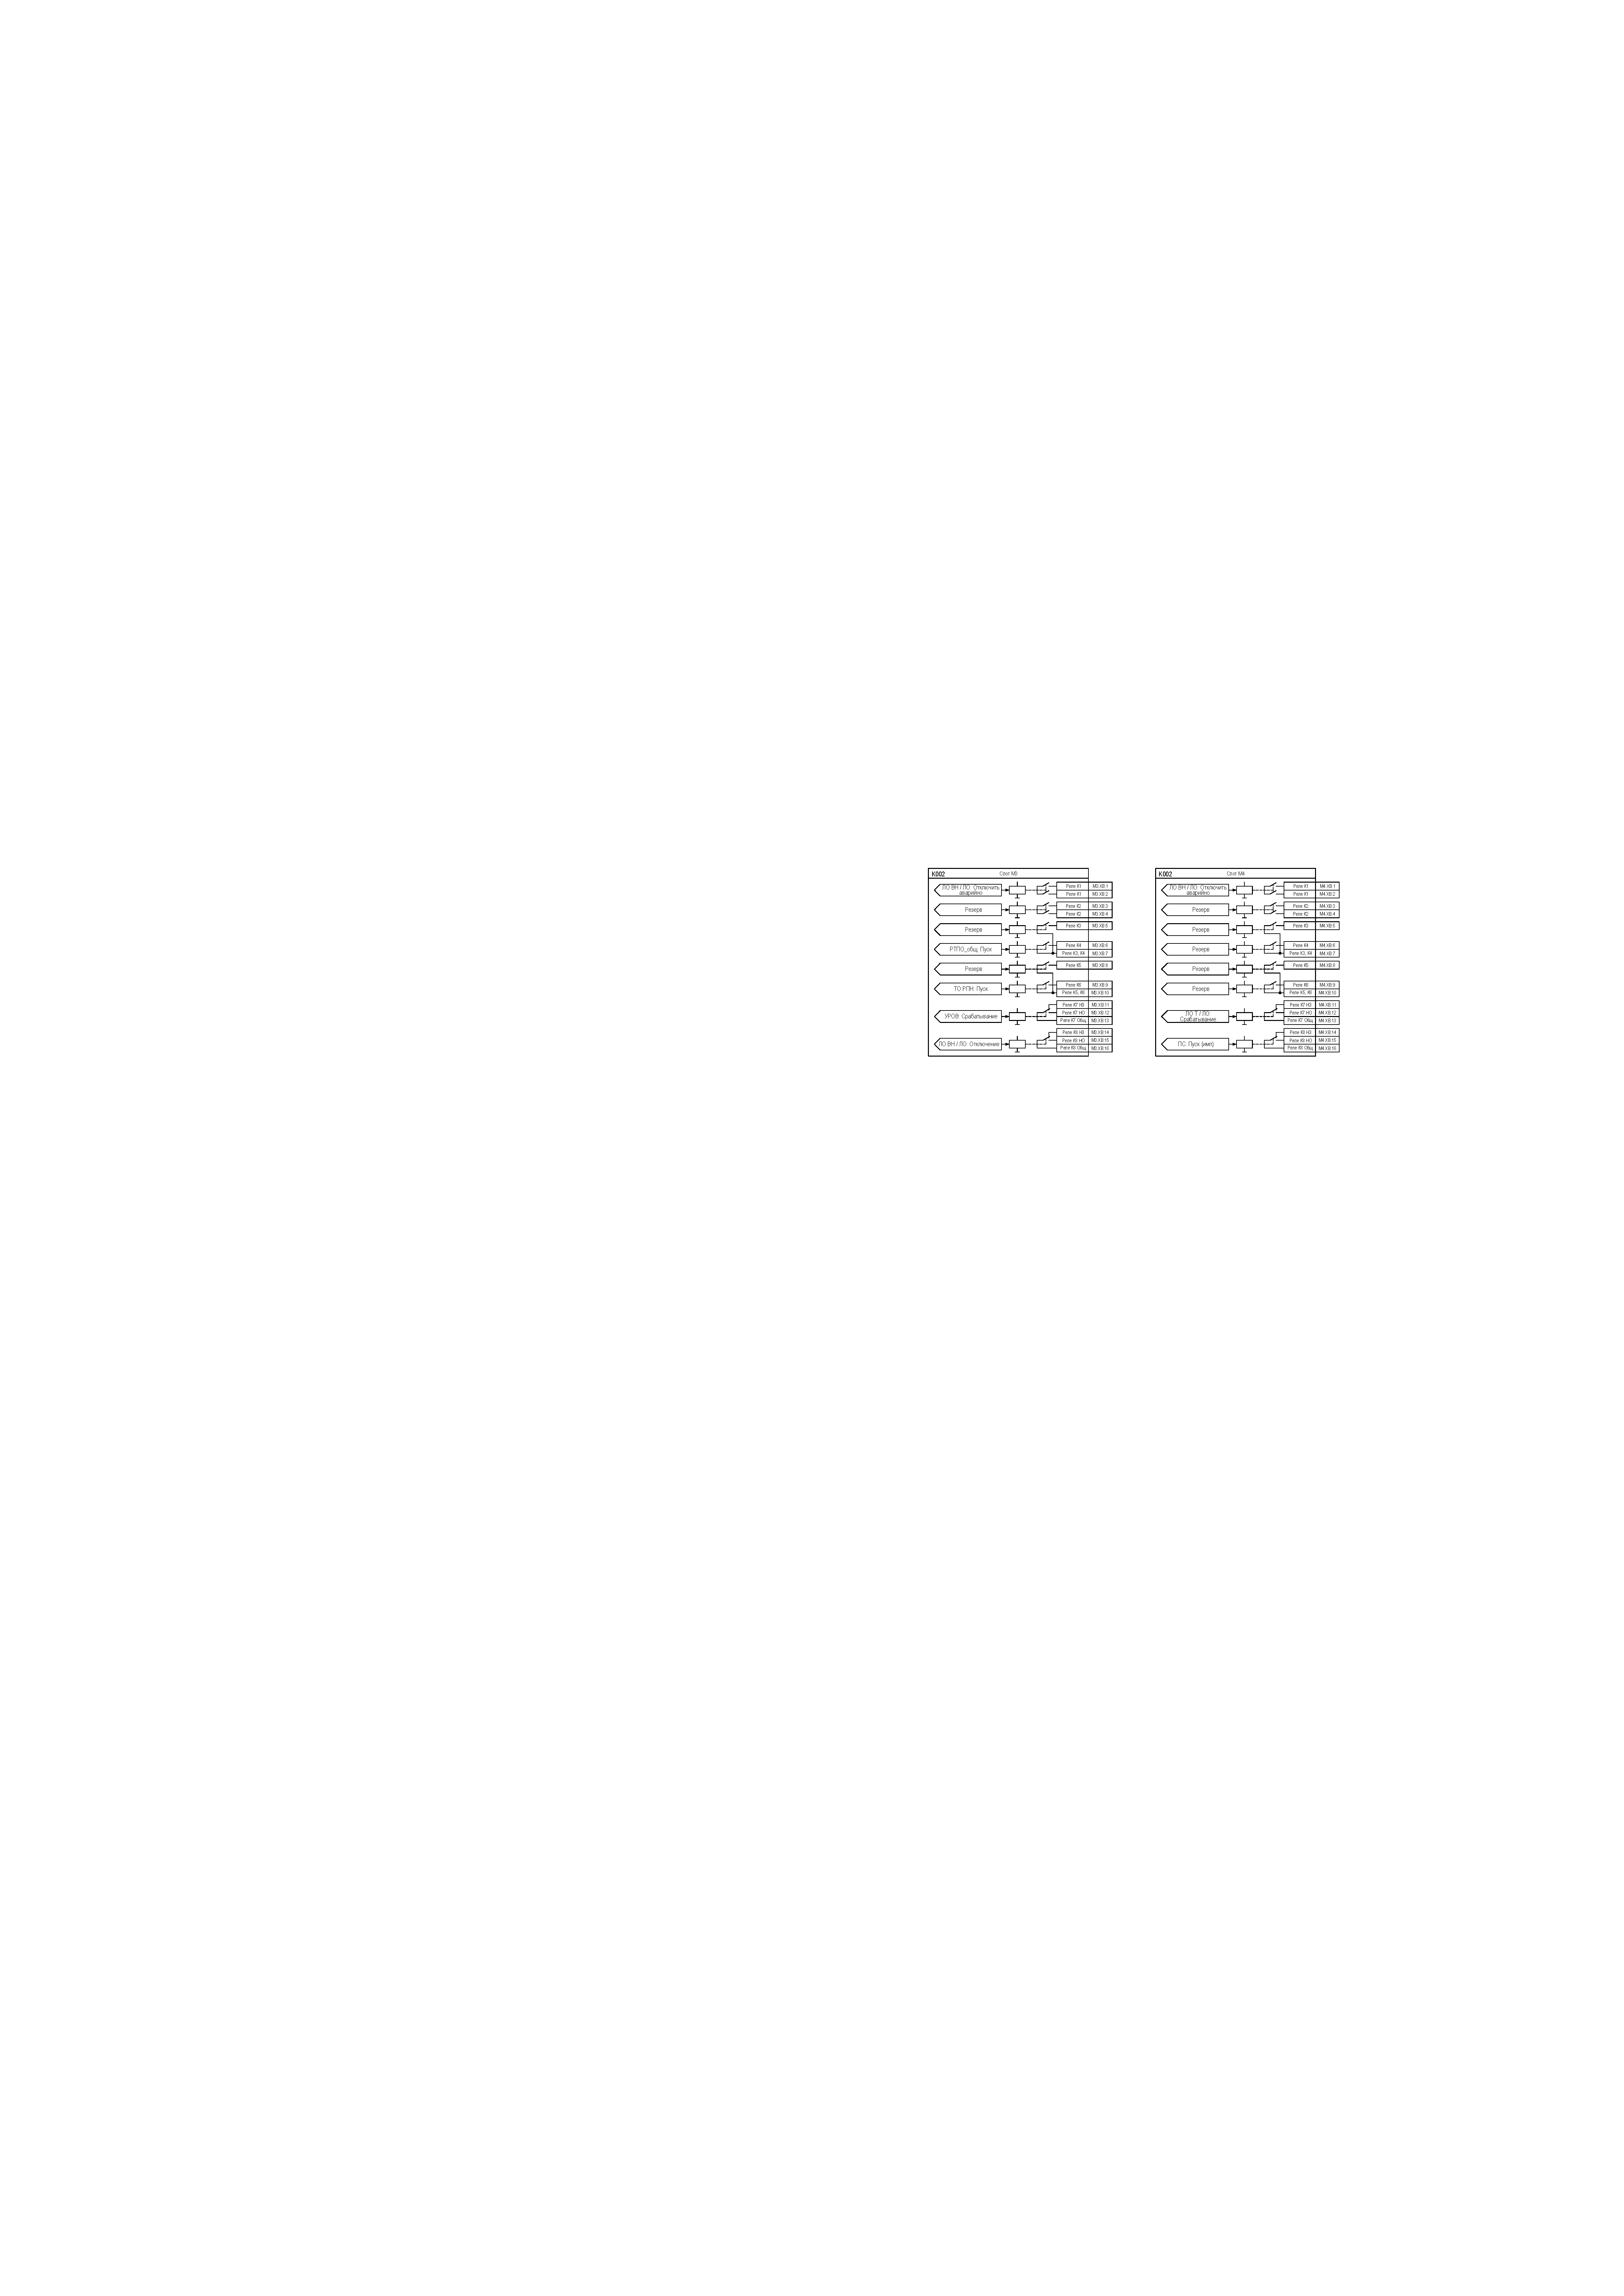
\includegraphics[width=1.5\textwidth]{img49.pdf}
  \caption{Подключение дискретных входов и выходов к внутренним сигналам алгоритмов для плат в слотах М3, М4}
  \label{fig:sig22} % Опционально: ссылка на рисунок
\end{figure}

\begin{figure}[h!]
  \centering
  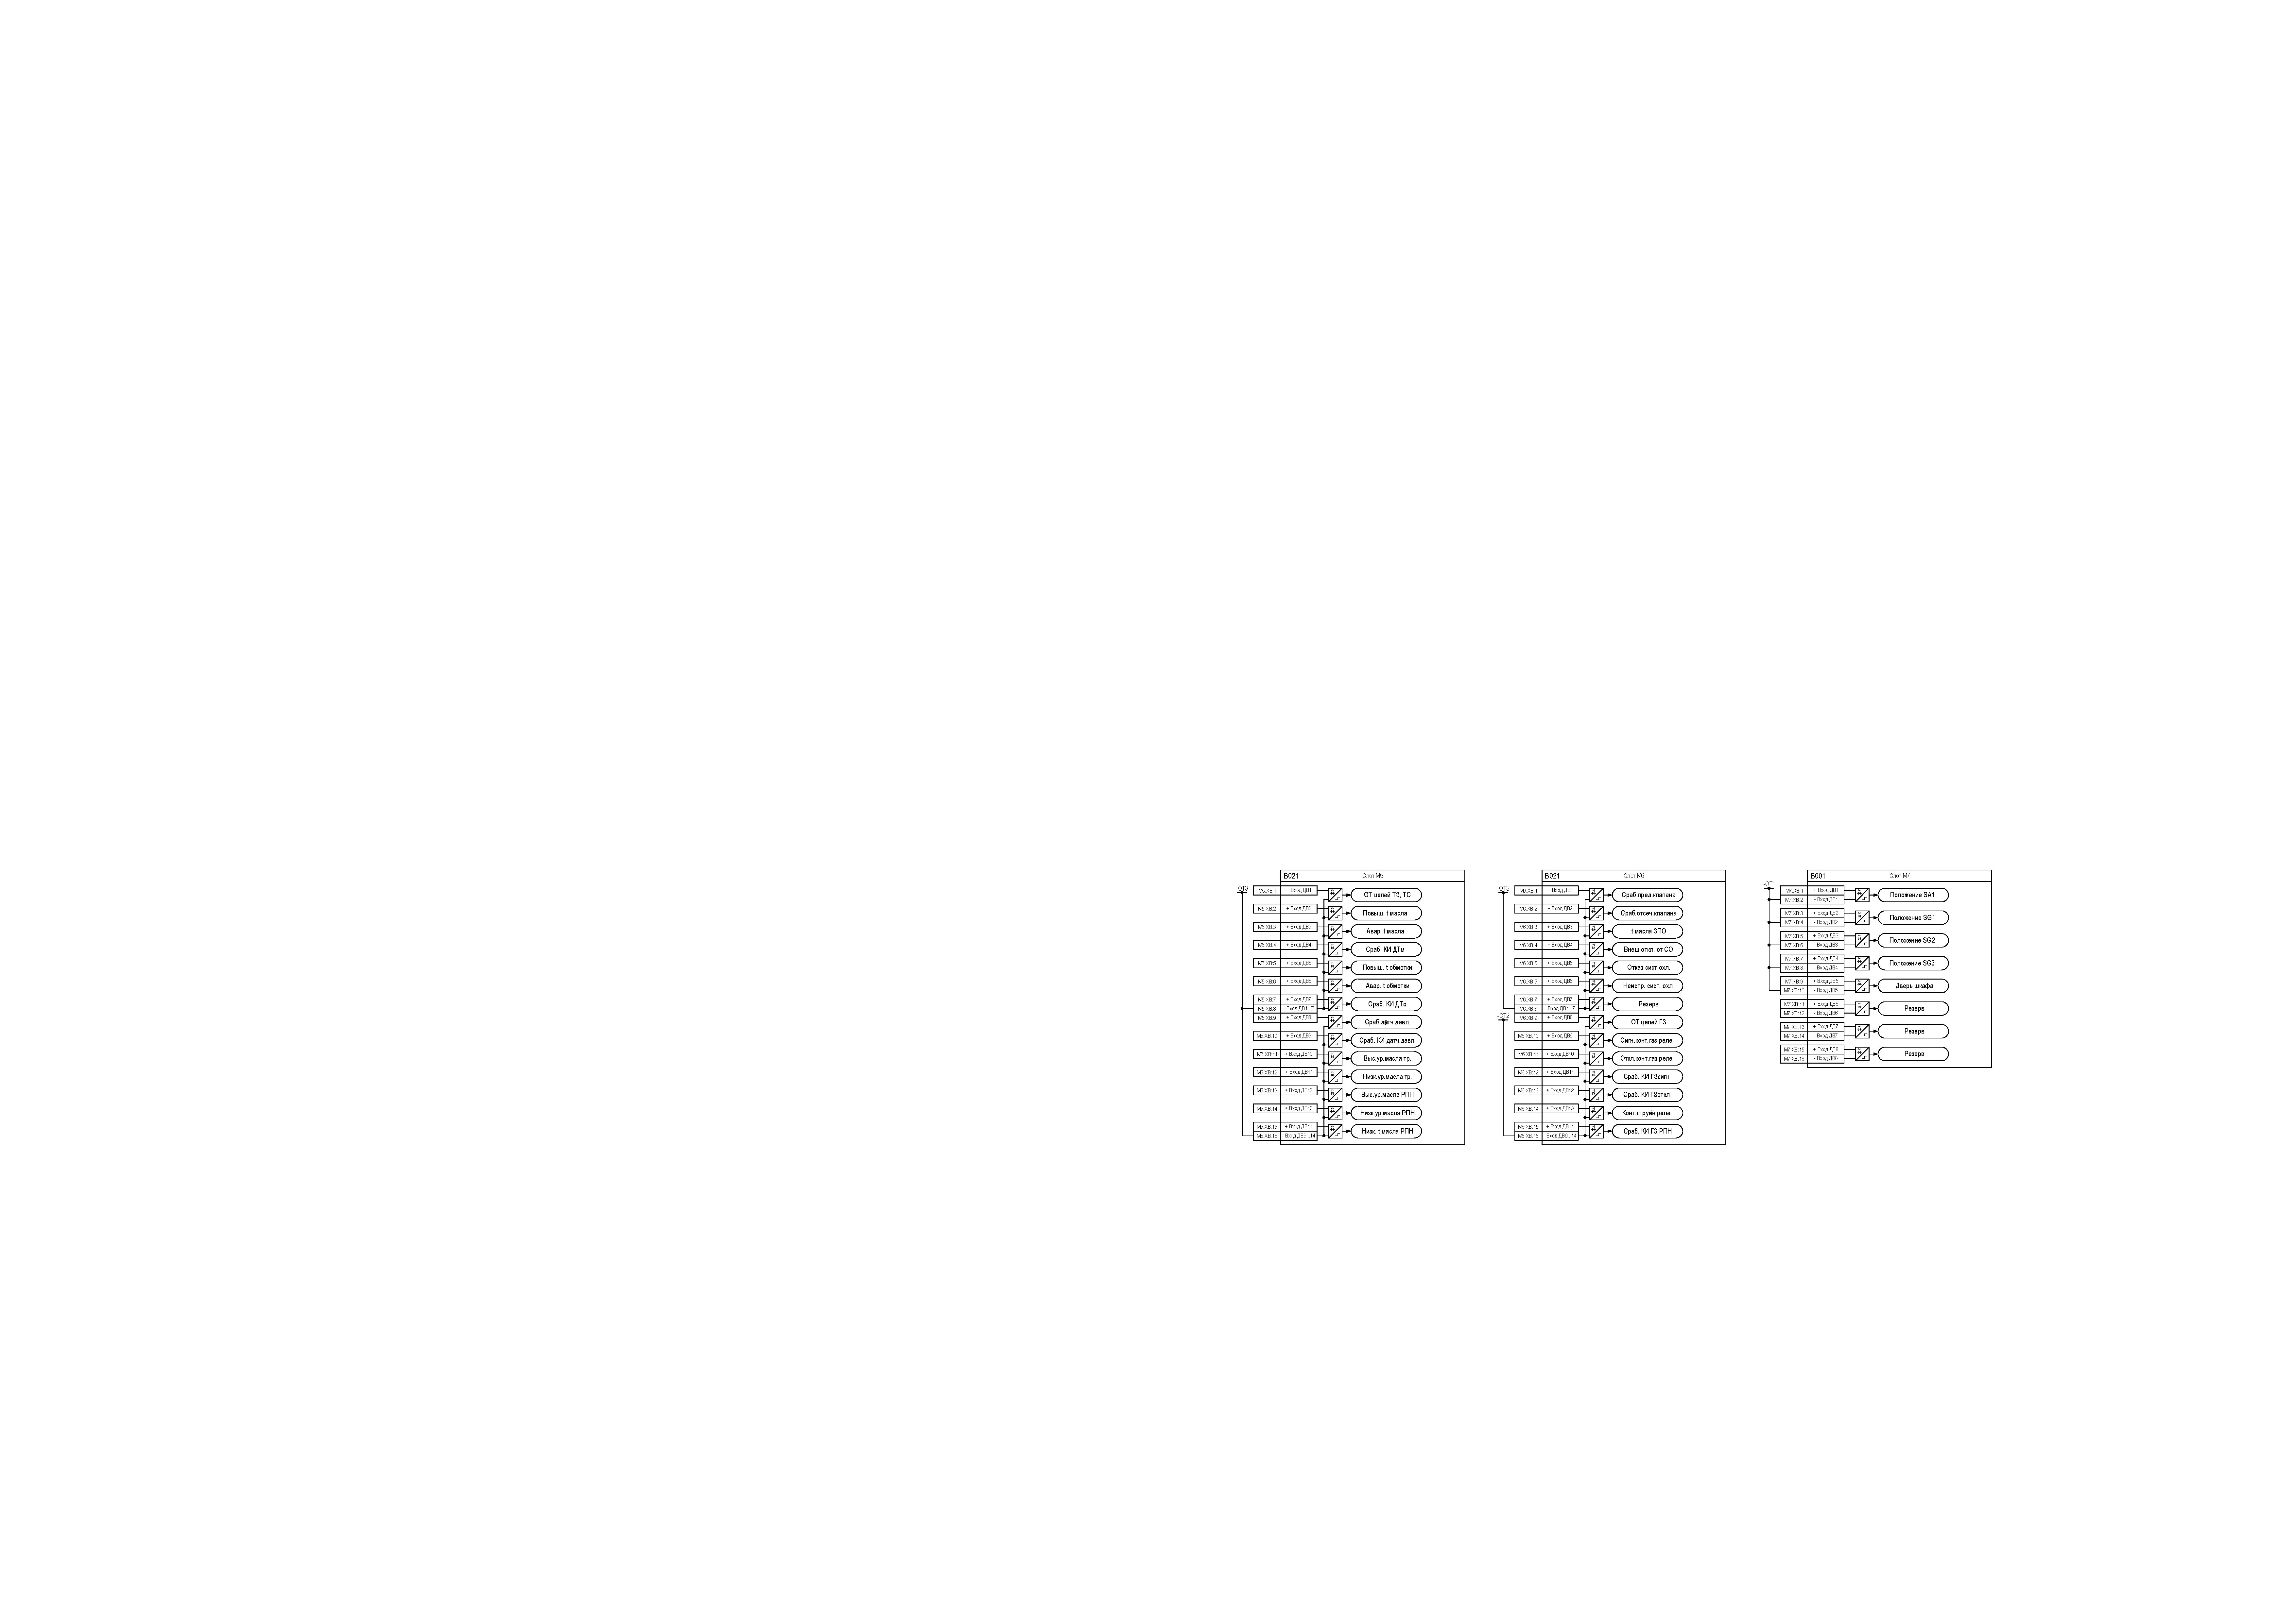
\includegraphics[width=1.45\textwidth]{img50.pdf}
  \caption{Подключение дискретных входов и выходов к внутренним сигналам алгоритмов для плат в слотах М5-М7}
  \label{fig:sig23} % Опционально: ссылка на рисунок
\end{figure}

\clearpage
\end{landscape}
\restoregeometry


\newpage
\KOMAoption{paper}{a4, portrait}
\areaset{180mm}{267mm}
\fancyheadoffset{0pt} % обновляем хедер и футер

\newgeometry{
  includehead,
  includefoot,
  nomarginpar,
  top=6mm,
  bottom=6mm,
  left=22mm,
  right=10mm,
  headheight=14.5pt,
  headsep=3mm,        % Добавить headsep
  footskip=7mm,
}


\color{uniblue}{\section[(рекомендуемое) Элементы функциональных схем]{(рекомендуемое)\\Элементы функциональных схем}\label{app:func_desc}}
\color{black}



\begin{longtable}{
|>{\centering\arraybackslash}m{5.5cm}
|>{\centering\arraybackslash}m{5.5cm}
|>{\centering\arraybackslash}m{5.5cm}
|}

\caption{Принятые обозначения элементов функциональных схем\hfill\vspace{-0.5\baselineskip}}\label{appEl:tbl1}\\ 

\hline
\rowcolor{gray!30}
Графическое отображение на схеме & Назначение & Примечание \\ 
\hline
\endfirsthead
\caption*{\hspace{3pt}\emph{Продолжение таблицы \ref{appEl:tbl1}\hfill\vspace{-0.5\baselineskip}}} \\ % сделано по ГОСТ 2.105 п.6.8.7
\hline
\rowcolor{gray!30}
Графическое отображение на схеме & Назначение & Примечание \\ 
\hline
\endhead

\hline
\endfoot

\hline
\endlastfoot

\centering {\includegraphics[width=0.2\textwidth,height=0.2\textheight,keepaspectratio]{img51.pdf}}& \centering Аналоговый канал & \centering \arraybackslash\\
\hline

\centering {\includegraphics[width=0.2\textwidth,height=0.2\textheight,keepaspectratio]{img52.pdf}} & \centering Пусковой (измерительный орган) & \centering \arraybackslash   \\
\hline

\centering {\includegraphics[width=0.2\textwidth,height=0.2\textheight,keepaspectratio]{img53.pdf}} & \centering Внешний входной сигнал (из матрицы входов/выходов) & \centering \arraybackslash   \\
\hline

\centering {\includegraphics[width=0.2\textwidth,height=0.2\textheight,keepaspectratio]{img54.pdf}} & \centering Входной сигнал от внутренней логики & \centering \arraybackslash   \\
\hline

\centering {\includegraphics[width=0.2\textwidth,height=0.2\textheight,keepaspectratio]{img55.pdf}} & \centering Выходной сигнал внутренней логики & \centering \arraybackslash   \\
\hline

\centering {\includegraphics[width=0.2\textwidth,height=0.2\textheight,keepaspectratio]{img56.pdf}} & \centering Входной сигнал от <<Виртуального ключа>> & \centering \arraybackslash   \\
\hline

\centering {\includegraphics[width=0.2\textwidth,height=0.2\textheight,keepaspectratio]{img57.pdf}} & \centering Входной сигнал от <<Виртуальной кнопки>> & \centering \arraybackslash   \\
\hline

\centering {\includegraphics[width=0.2\textwidth,height=0.2\textheight,keepaspectratio]{img58.pdf}} & \centering Программный переключатель & \centering \arraybackslash   \\
\hline

\centering {\includegraphics[width=0.2\textwidth,height=0.2\textheight,keepaspectratio]{img59.pdf}} & \centering Логический элемент <<И>> & \centering \arraybackslash 
  {\includegraphics[width=0.1\textwidth,height=0.1\textheight,keepaspectratio]{img60.pdf}} \\
\hline

\centering {\includegraphics[width=0.2\textwidth,height=0.2\textheight,keepaspectratio]{img61.pdf}} & \centering Логический элемент <<ИЛИ>> & \centering \arraybackslash 
  {\includegraphics[width=0.1\textwidth,height=0.1\textheight,keepaspectratio]{img62.pdf}} \\
\hline

\centering {\includegraphics[width=0.2\textwidth,height=0.2\textheight,keepaspectratio]{img63.pdf}} & \centering Логический элемент <<ИСКЛЮЧАЮЩЕЕ ИЛИ>> & \centering \arraybackslash 
  {\includegraphics[width=0.1\textwidth,height=0.1\textheight,keepaspectratio]{img64.pdf}} \\
\hline

\centering {\includegraphics[width=0.2\textwidth,height=0.2\textheight,keepaspectratio]{img65.pdf}} & \centering SR-триггер & \multirow{2}{*} 
  {\includegraphics[width=0.1\textwidth,height=0.1\textheight,keepaspectratio]{img66.pdf}} \\
\cline{1-2}

\centering {\includegraphics[width=0.2\textwidth,height=0.2\textheight,keepaspectratio]{img67.pdf}} & \centering SR-триггер с сохранением состояния после исчезновения питания & \centering \arraybackslash   \\
\hline

\centering {\includegraphics[width=0.2\textwidth,height=0.2\textheight,keepaspectratio]{img68.pdf}} & \centering RS-триггер & \multirow{2}{*} 
  {\includegraphics[width=0.1\textwidth,height=0.1\textheight,keepaspectratio]{img69.pdf}} \\
\cline{1-2}

\centering {\includegraphics[width=0.2\textwidth,height=0.2\textheight,keepaspectratio]{img70.pdf}} & \centering RS-триггер с сохранением состояния после исчезновения питания & \centering \arraybackslash   \\
\hline

\centering {\includegraphics[width=0.2\textwidth,height=0.2\textheight,keepaspectratio]{img71.pdf}}& \centering Логический элемент <<НЕ>> & \centering \arraybackslash\\
\hline

\centering {\includegraphics[width=0.2\textwidth,height=0.2\textheight,keepaspectratio]{img72.pdf}} & \centering Выдержка времени на срабатывание (регулируемая) & \multirow{2}{*} 
  {\includegraphics[width=0.23\textwidth,height=0.23\textheight,keepaspectratio]{img73.pdf}} \\
\cline{1-2}

\centering {\includegraphics[width=0.2\textwidth,height=0.2\textheight,keepaspectratio]{img74.pdf}} & \centering Выдержка времени на срабатывание (нерегулируемая) & \centering \arraybackslash   \\
\hline

\centering {\includegraphics[width=0.2\textwidth,height=0.2\textheight,keepaspectratio]{img75.pdf}} & \centering Выдержка времени на возврат (регулируемая) & \multirow{2}{*} 
  {\includegraphics[width=0.23\textwidth,height=0.23\textheight,keepaspectratio]{img76.pdf}} \\
\cline{1-2}

\centering {\includegraphics[width=0.2\textwidth,height=0.2\textheight,keepaspectratio]{img77.pdf}} & \centering Выдержка времени на возврат (нерегулируемая) & \centering \arraybackslash   \\
\hline

\centering {\includegraphics[width=0.2\textwidth,height=0.2\textheight,keepaspectratio]{img78.pdf}} & \centering Одновибратор по переднему фронту без перезапуска (регулируемый) & \multirow{2}{*} 
  {\includegraphics[width=0.23\textwidth,height=0.23\textheight,keepaspectratio]{img79.pdf}} \\
\cline{1-2}

\centering {\includegraphics[width=0.2\textwidth,height=0.2\textheight,keepaspectratio]{img80.pdf}} & \centering Одновибратор по переднему фронту без перезапуска (нерегулируемый) & \centering \arraybackslash   \\
\hline

\centering {\includegraphics[width=0.2\textwidth,height=0.2\textheight,keepaspectratio]{img81.pdf}} & \centering Одновибратор по переднему фронту со сбросом (регулируемый) & \centering \arraybackslash 
  {\includegraphics[width=0.2\textwidth,height=0.2\textheight,keepaspectratio]{img82.pdf}} \\
\hline

\centering {\includegraphics[width=0.2\textwidth,height=0.2\textheight,keepaspectratio]{img83.pdf}} & \centering Одновибратор по заднему фронту без перезапуска (нерегулируемый) & \centering \arraybackslash 
  {\includegraphics[width=0.2\textwidth,height=0.2\textheight,keepaspectratio]{img84.pdf}} \\
\hline

\centering {\includegraphics[width=0.2\textwidth,height=0.2\textheight,keepaspectratio]{img85.pdf}} & \centering Выбор максимального значения & \centering \arraybackslash   \\
\hline

\centering {\includegraphics[width=0.2\textwidth,height=0.2\textheight,keepaspectratio]{img86.pdf}} & \centering Выбор минимального значения & \centering \arraybackslash   \\
\hline

\centering {\includegraphics[width=0.2\textwidth,height=0.2\textheight,keepaspectratio]{img87.pdf}} & \centering Пороговый элемент с гистерезисом (сравнение с уставкой) & \centering \arraybackslash   \\
\hline

\end{longtable} 

\restoregeometry\resettocdepth % восстановление уровня оглавления
\end{appendices}

\newpage
\KOMAoption{paper}{a4, portrait}
\areaset{180mm}{267mm}
\fancyheadoffset{0pt} % обновляем хедер и футер

\newgeometry{
  includehead,
  includefoot,
  nomarginpar,
  top=6mm,
  bottom=6mm,
  left=22mm,
  right=10mm,
  headheight=14.5pt,
  headsep=3mm,        % Добавить headsep
  footskip=7mm,
}

\begin{longtable}{|>{\centering\arraybackslash}m{0.6cm}|>{\centering\arraybackslash}m{1.8cm}|>{\centering\arraybackslash}m{1.8cm}|>{\centering\arraybackslash}m{1.8cm}|>{\centering\arraybackslash}m{1.8cm}|>{\centering\arraybackslash}m{1.8cm}|>{\centering\arraybackslash}m{2.2cm}|>{\centering\arraybackslash}m{1.1cm}|>{\centering\arraybackslash}m{1cm}|}
\hline

\multicolumn{9}{|c|}{Лист регистрации изменений} \\
\cline{1-9}
\multirow{2}{*}{} & \multicolumn{4}{c|}{Номера листов (страниц)} & & & & \\
\cline{2-5}
Изм.& измененных & замененных & новых & аннулированных &  Всего листов (страниц) в документе & № документа & Подп. & Дата \\
\hline
\endfirsthead
{\emph{Продолжение\hfill\vspace{-0.5\baselineskip}}} \\ % Отступ обозначения таблицы от таблицы и выравнивание надписи слева
\hline
\multirow{2}{*}{} & \multicolumn{4}{c|}{Номера листов (страниц)} & & & & \\
\cline{2-5}
Изм.& измененных & замененных & новых & аннулированных &  Всего листов (страниц) в документе & № докум. & Подп. & Дата \\
\hline
\endhead
\hline
\endfoot
\hline
\endlastfoot

\centering   & \centering   & \centering   & \centering   & \centering   & \centering   & \centering   & \centering   & \centering\arraybackslash   \\[2\jot]  
\hline
\centering   & \centering   & \centering   & \centering   & \centering   & \centering   & \centering   & \centering   & \centering\arraybackslash   \\[2\jot]
\hline
\centering   & \centering   & \centering   & \centering   & \centering   & \centering   & \centering   & \centering   & \centering\arraybackslash   \\[2\jot]
\hline
\centering   & \centering   & \centering   & \centering   & \centering   & \centering   & \centering   & \centering   & \centering\arraybackslash   \\[2\jot]
\hline
\centering   & \centering   & \centering   & \centering   & \centering   & \centering   & \centering   & \centering   & \centering\arraybackslash   \\[2\jot]
\hline
\centering   & \centering   & \centering   & \centering   & \centering   & \centering   & \centering   & \centering   & \centering\arraybackslash   \\[2\jot]
\hline
\centering   & \centering   & \centering   & \centering   & \centering   & \centering   & \centering   & \centering   & \centering\arraybackslash   \\[2\jot]
\hline
\centering   & \centering   & \centering   & \centering   & \centering   & \centering   & \centering   & \centering   & \centering\arraybackslash   \\[2\jot]
\hline
\centering   & \centering   & \centering   & \centering   & \centering   & \centering   & \centering   & \centering   & \centering\arraybackslash   \\[2\jot]
\hline
\centering   & \centering   & \centering   & \centering   & \centering   & \centering   & \centering   & \centering   & \centering\arraybackslash   \\[2\jot]
\hline
\centering   & \centering   & \centering   & \centering   & \centering   & \centering   & \centering   & \centering   & \centering\arraybackslash   \\[2\jot]
\hline
\centering   & \centering   & \centering   & \centering   & \centering   & \centering   & \centering   & \centering   & \centering\arraybackslash   \\[2\jot]
\hline
\centering   & \centering   & \centering   & \centering   & \centering   & \centering   & \centering   & \centering   & \centering\arraybackslash   \\[2\jot]
\hline
\centering   & \centering   & \centering   & \centering   & \centering   & \centering   & \centering   & \centering   & \centering\arraybackslash   \\[2\jot]
\hline
\centering   & \centering   & \centering   & \centering   & \centering   & \centering   & \centering   & \centering   & \centering\arraybackslash   \\[2\jot]
\hline
\centering   & \centering   & \centering   & \centering   & \centering   & \centering   & \centering   & \centering   & \centering\arraybackslash   \\[2\jot]
\hline
\centering   & \centering   & \centering   & \centering   & \centering   & \centering   & \centering   & \centering   & \centering\arraybackslash   \\[2\jot]
\hline
\centering   & \centering   & \centering   & \centering   & \centering   & \centering   & \centering   & \centering   & \centering\arraybackslash   \\[2\jot]
\hline
\centering   & \centering   & \centering   & \centering   & \centering   & \centering   & \centering   & \centering   & \centering\arraybackslash   \\[2\jot]
\hline
\centering   & \centering   & \centering   & \centering   & \centering   & \centering   & \centering   & \centering   & \centering\arraybackslash   \\[2\jot]
\hline
\centering   & \centering   & \centering   & \centering   & \centering   & \centering   & \centering   & \centering   & \centering\arraybackslash   \\[2\jot]
\hline
\centering   & \centering   & \centering   & \centering   & \centering   & \centering   & \centering   & \centering   & \centering\arraybackslash   \\[2\jot]
\hline
\centering   & \centering   & \centering   & \centering   & \centering   & \centering   & \centering   & \centering   & \centering\arraybackslash   \\[2\jot]
\hline
\centering   & \centering   & \centering   & \centering   & \centering   & \centering   & \centering   & \centering   & \centering\arraybackslash   \\[2\jot]
\hline
\centering   & \centering   & \centering   & \centering   & \centering   & \centering   & \centering   & \centering   & \centering\arraybackslash   \\[2\jot]
\hline
\centering   & \centering   & \centering   & \centering   & \centering   & \centering   & \centering   & \centering   & \centering\arraybackslash   \\[2\jot]
\hline
\centering   & \centering   & \centering   & \centering   & \centering   & \centering   & \centering   & \centering   & \centering\arraybackslash   \\[2\jot]
\hline
\end{longtable}



\restoregeometry %=======================================
\end{document}
